\documentclass[twoside]{book}

% Packages required by doxygen
\usepackage{calc}
\usepackage{doxygen}
\usepackage{graphicx}
\usepackage[utf8]{inputenc}
\usepackage{makeidx}
\usepackage{multicol}
\usepackage{multirow}
\usepackage{textcomp}
\usepackage[table]{xcolor}

% Font selection
\usepackage[T1]{fontenc}
\usepackage{mathptmx}
\usepackage[scaled=.90]{helvet}
\usepackage{courier}
\usepackage{amssymb}
\usepackage{sectsty}
\renewcommand{\familydefault}{\sfdefault}
\allsectionsfont{%
  \fontseries{bc}\selectfont%
  \color{darkgray}%
}
\renewcommand{\DoxyLabelFont}{%
  \fontseries{bc}\selectfont%
  \color{darkgray}%
}

% Page & text layout
\usepackage{geometry}
\geometry{%
  a4paper,%
  top=2.5cm,%
  bottom=2.5cm,%
  left=2.5cm,%
  right=2.5cm%
}
\tolerance=750
\hfuzz=15pt
\hbadness=750
\setlength{\emergencystretch}{15pt}
\setlength{\parindent}{0cm}
\setlength{\parskip}{0.2cm}
\makeatletter
\renewcommand{\paragraph}{%
  \@startsection{paragraph}{4}{0ex}{-1.0ex}{1.0ex}{%
    \normalfont\normalsize\bfseries\SS@parafont%
  }%
}
\renewcommand{\subparagraph}{%
  \@startsection{subparagraph}{5}{0ex}{-1.0ex}{1.0ex}{%
    \normalfont\normalsize\bfseries\SS@subparafont%
  }%
}
\makeatother

% Headers & footers
\usepackage{fancyhdr}
\pagestyle{fancyplain}
\fancyhead[LE]{\fancyplain{}{\bfseries\thepage}}
\fancyhead[CE]{\fancyplain{}{}}
\fancyhead[RE]{\fancyplain{}{\bfseries\leftmark}}
\fancyhead[LO]{\fancyplain{}{\bfseries\rightmark}}
\fancyhead[CO]{\fancyplain{}{}}
\fancyhead[RO]{\fancyplain{}{\bfseries\thepage}}
\fancyfoot[LE]{\fancyplain{}{}}
\fancyfoot[CE]{\fancyplain{}{}}
\fancyfoot[RE]{\fancyplain{}{\bfseries\scriptsize Generated on Wed Dec 2 2015 18\-:58\-:54 for Optimal Partition by Doxygen }}
\fancyfoot[LO]{\fancyplain{}{\bfseries\scriptsize Generated on Wed Dec 2 2015 18\-:58\-:54 for Optimal Partition by Doxygen }}
\fancyfoot[CO]{\fancyplain{}{}}
\fancyfoot[RO]{\fancyplain{}{}}
\renewcommand{\footrulewidth}{0.4pt}
\renewcommand{\chaptermark}[1]{%
  \markboth{#1}{}%
}
\renewcommand{\sectionmark}[1]{%
  \markright{\thesection\ #1}%
}

% Indices & bibliography
\usepackage{natbib}
\usepackage[titles]{tocloft}
\setcounter{tocdepth}{3}
\setcounter{secnumdepth}{5}
\makeindex

% Hyperlinks (required, but should be loaded last)
\usepackage{ifpdf}
\ifpdf
  \usepackage[pdftex,pagebackref=true]{hyperref}
\else
  \usepackage[ps2pdf,pagebackref=true]{hyperref}
\fi
\hypersetup{%
  colorlinks=true,%
  linkcolor=blue,%
  citecolor=blue,%
  unicode%
}

% Custom commands
\newcommand{\clearemptydoublepage}{%
  \newpage{\pagestyle{empty}\cleardoublepage}%
}


%===== C O N T E N T S =====

\begin{document}

% Titlepage & ToC
\hypersetup{pageanchor=false}
\pagenumbering{roman}
\begin{titlepage}
\vspace*{7cm}
\begin{center}%
{\Large Optimal Partition }\\
\vspace*{1cm}
{\large Generated by Doxygen 1.8.6}\\
\vspace*{0.5cm}
{\small Wed Dec 2 2015 18:58:54}\\
\end{center}
\end{titlepage}
\clearemptydoublepage
\tableofcontents
\clearemptydoublepage
\pagenumbering{arabic}
\hypersetup{pageanchor=true}

%--- Begin generated contents ---
\chapter{Main Page}
\label{index}\hypertarget{index}{}This program is a toolbox to solve special versions of the Set Partitioning Problem, that is the combinatorial optimisation of a decomposable objective over a set of feasible partitions (defined according to specific algebraic structures\-: e.\-g., hierachies, sets of intervals, graphs). The objectives are mainly based on information theory, in the perspective of multilevel analysis of large-\/scale datasets, and the algorithms are based on dynamic programming. For details regarding the formal grounds of this work, please refer to\-:

Robin Lamarche-\/\-Perrin, Yves Demazeau and Jean-\/\-Marc Vincent. A Generic Set Partitioning Algorithm with Applications to Hierarchical and Ordered Sets. Technical Report 105/2014, Max-\/\-Planck-\/\-Institute for Mathematics in the Sciences, Leipzig, Germany, May 2014.

\href{http://www.mis.mpg.de/publications/preprints/2014/prepr2014-105.html}{\tt http\-://www.\-mis.\-mpg.\-de/publications/preprints/2014/prepr2014-\/105.\-html}

Copyright © 2015 Robin Lamarche-\/\-Perrin (\href{mailto:Robin.Lamarche-Perrin@lip6.fr}{\tt Robin.\-Lamarche-\/\-Perrin@lip6.\-fr})

This program is free software\-: you can redistribute it and/or modify it under the terms of the G\-N\-U General Public License as published by the Free Software Foundation, either version 3 of the License, or (at your option) any later version.

This program is distributed in the hope that it will be useful, but W\-I\-T\-H\-O\-U\-T A\-N\-Y W\-A\-R\-R\-A\-N\-T\-Y; without even the implied warranty of M\-E\-R\-C\-H\-A\-N\-T\-A\-B\-I\-L\-I\-T\-Y or F\-I\-T\-N\-E\-S\-S F\-O\-R A P\-A\-R\-T\-I\-C\-U\-L\-A\-R P\-U\-R\-P\-O\-S\-E. See the G\-N\-U General Public License for more details.

You should have received a copy of the G\-N\-U General Public License along with this program. If not, see \href{http://www.gnu.org/licenses/}{\tt http\-://www.\-gnu.\-org/licenses/}. 
\chapter{Hierarchical Index}
\section{Class Hierarchy}
This inheritance list is sorted roughly, but not completely, alphabetically\-:\begin{DoxyCompactList}
\item \contentsline{section}{Abstract\-Set}{\pageref{classAbstractSet}}{}
\begin{DoxyCompactList}
\item \contentsline{section}{Bi\-Set}{\pageref{classBiSet}}{}
\item \contentsline{section}{Graph}{\pageref{classGraph}}{}
\begin{DoxyCompactList}
\item \contentsline{section}{Complete\-Graph}{\pageref{classCompleteGraph}}{}
\item \contentsline{section}{Filiform\-Graph}{\pageref{classFiliformGraph}}{}
\item \contentsline{section}{Random\-Graph}{\pageref{classRandomGraph}}{}
\item \contentsline{section}{Ring\-Graph}{\pageref{classRingGraph}}{}
\end{DoxyCompactList}
\item \contentsline{section}{Hierarchical\-Hierarchical\-Set}{\pageref{classHierarchicalHierarchicalSet}}{}
\item \contentsline{section}{Hierarchical\-Ordered\-Set}{\pageref{classHierarchicalOrderedSet}}{}
\item \contentsline{section}{Hierarchical\-Set}{\pageref{classHierarchicalSet}}{}
\item \contentsline{section}{Multi\-Set}{\pageref{classMultiSet}}{}
\item \contentsline{section}{N\-H\-O\-Set}{\pageref{classNHOSet}}{}
\item \contentsline{section}{Nonconstrained\-Ordered\-Set}{\pageref{classNonconstrainedOrderedSet}}{}
\item \contentsline{section}{Nonconstrained\-Set}{\pageref{classNonconstrainedSet}}{}
\item \contentsline{section}{Ordered\-Set}{\pageref{classOrderedSet}}{}
\item \contentsline{section}{Ring}{\pageref{classRing}}{}
\end{DoxyCompactList}
\item \contentsline{section}{Bi\-Subset}{\pageref{classBiSubset}}{}
\item \contentsline{section}{Data\-Point\-Struct}{\pageref{structDataPointStruct}}{}
\item \contentsline{section}{Dataset}{\pageref{classDataset}}{}
\item \contentsline{section}{Datatree}{\pageref{classDatatree}}{}
\item \contentsline{section}{Graph\-Component}{\pageref{classGraphComponent}}{}
\item \contentsline{section}{H\-H\-Node}{\pageref{classHHNode}}{}
\item \contentsline{section}{H\-Node}{\pageref{classHNode}}{}
\item \contentsline{section}{H\-O\-Node}{\pageref{classHONode}}{}
\item \contentsline{section}{Markov\-Data\-Set}{\pageref{classMarkovDataSet}}{}
\item \contentsline{section}{Markov\-Process}{\pageref{classMarkovProcess}}{}
\item \contentsline{section}{Markov\-Trajectory}{\pageref{classMarkovTrajectory}}{}
\item \contentsline{section}{Multi\-Subset}{\pageref{classMultiSubset}}{}
\item \contentsline{section}{N\-H\-O\-Node}{\pageref{classNHONode}}{}
\item \contentsline{section}{Objective\-Function}{\pageref{classObjectiveFunction}}{}
\begin{DoxyCompactList}
\item \contentsline{section}{Information\-Bottleneck}{\pageref{classInformationBottleneck}}{}
\item \contentsline{section}{Logarithmic\-Score}{\pageref{classLogarithmicScore}}{}
\item \contentsline{section}{Relative\-Entropy}{\pageref{classRelativeEntropy}}{}
\end{DoxyCompactList}
\item \contentsline{section}{Objective\-Value}{\pageref{classObjectiveValue}}{}
\begin{DoxyCompactList}
\item \contentsline{section}{Bottleneck\-Objective\-Value}{\pageref{classBottleneckObjectiveValue}}{}
\item \contentsline{section}{Logarithmic\-Score\-Value}{\pageref{classLogarithmicScoreValue}}{}
\item \contentsline{section}{Relative\-Objective\-Value}{\pageref{classRelativeObjectiveValue}}{}
\end{DoxyCompactList}
\item \contentsline{section}{Ordered\-Datatree}{\pageref{classOrderedDatatree}}{}
\item \contentsline{section}{Ordered\-Partition}{\pageref{classOrderedPartition}}{}
\item \contentsline{section}{Part}{\pageref{classPart}}{}
\begin{DoxyCompactList}
\item \contentsline{section}{Bi\-Part}{\pageref{classBiPart}}{}
\item \contentsline{section}{Multi\-Part}{\pageref{classMultiPart}}{}
\end{DoxyCompactList}
\item \contentsline{section}{Partition}{\pageref{classPartition}}{}
\item \contentsline{section}{Prediction\-Dataset}{\pageref{classPredictionDataset}}{}
\item \contentsline{section}{Timer}{\pageref{classTimer}}{}
\item \contentsline{section}{Tree\-To\-Add}{\pageref{structTreeToAdd}}{}
\item \contentsline{section}{Uni\-Set}{\pageref{classUniSet}}{}
\begin{DoxyCompactList}
\item \contentsline{section}{Graph\-Based\-Uni\-Set}{\pageref{classGraphBasedUniSet}}{}
\item \contentsline{section}{Hierarchical\-Uni\-Set}{\pageref{classHierarchicalUniSet}}{}
\item \contentsline{section}{Ordered\-Uni\-Set}{\pageref{classOrderedUniSet}}{}
\end{DoxyCompactList}
\item \contentsline{section}{Uni\-Subset}{\pageref{classUniSubset}}{}
\item \contentsline{section}{Voter\-Binning}{\pageref{classVoterBinning}}{}
\item \contentsline{section}{Voter\-Data\-Set}{\pageref{classVoterDataSet}}{}
\item \contentsline{section}{Voter\-Edge}{\pageref{classVoterEdge}}{}
\item \contentsline{section}{Voter\-Graph}{\pageref{classVoterGraph}}{}
\begin{DoxyCompactList}
\item \contentsline{section}{Chain\-Voter\-Graph}{\pageref{classChainVoterGraph}}{}
\item \contentsline{section}{Complete\-Voter\-Graph}{\pageref{classCompleteVoterGraph}}{}
\item \contentsline{section}{Two\-Communities\-Voter\-Graph}{\pageref{classTwoCommunitiesVoterGraph}}{}
\end{DoxyCompactList}
\item \contentsline{section}{Voter\-Measurement}{\pageref{classVoterMeasurement}}{}
\begin{DoxyCompactList}
\item \contentsline{section}{Empty\-Voter\-Measurement}{\pageref{classEmptyVoterMeasurement}}{}
\item \contentsline{section}{Macro\-Voter\-Measurement}{\pageref{classMacroVoterMeasurement}}{}
\item \contentsline{section}{Micro\-Voter\-Measurement}{\pageref{classMicroVoterMeasurement}}{}
\end{DoxyCompactList}
\item \contentsline{section}{Voter\-Measurement\-State}{\pageref{classVoterMeasurementState}}{}
\item \contentsline{section}{Voter\-Measurement\-Trajectory}{\pageref{classVoterMeasurementTrajectory}}{}
\item \contentsline{section}{Voter\-Node}{\pageref{classVoterNode}}{}
\item \contentsline{section}{Voter\-Probe}{\pageref{classVoterProbe}}{}
\item \contentsline{section}{Voter\-State}{\pageref{classVoterState}}{}
\item \contentsline{section}{Voter\-Trajectory}{\pageref{classVoterTrajectory}}{}
\end{DoxyCompactList}

\chapter{Class Index}
\section{Class List}
Here are the classes, structs, unions and interfaces with brief descriptions\-:\begin{DoxyCompactList}
\item\contentsline{section}{\hyperlink{classAbstractSet}{Abstract\-Set} \\*Abstract class defining a set of elements that one wants to partition while optimising some (decomposable) objective and preserving some algebraic constraints (set of feasible parts) }{\pageref{classAbstractSet}}{}
\item\contentsline{section}{\hyperlink{classAggregate}{Aggregate} }{\pageref{classAggregate}}{}
\item\contentsline{section}{\hyperlink{classAggregate2D}{Aggregate2\-D} }{\pageref{classAggregate2D}}{}
\item\contentsline{section}{\hyperlink{classBiPart}{Bi\-Part} }{\pageref{classBiPart}}{}
\item\contentsline{section}{\hyperlink{classBottleneckObjectiveValue}{Bottleneck\-Objective\-Value} }{\pageref{classBottleneckObjectiveValue}}{}
\item\contentsline{section}{\hyperlink{classCompleteGraph}{Complete\-Graph} }{\pageref{classCompleteGraph}}{}
\item\contentsline{section}{\hyperlink{structDataPointStruct}{Data\-Point\-Struct} }{\pageref{structDataPointStruct}}{}
\item\contentsline{section}{\hyperlink{classDataset}{Dataset} }{\pageref{classDataset}}{}
\item\contentsline{section}{\hyperlink{classDatatree}{Datatree} }{\pageref{classDatatree}}{}
\item\contentsline{section}{\hyperlink{classFiliformGraph}{Filiform\-Graph} }{\pageref{classFiliformGraph}}{}
\item\contentsline{section}{\hyperlink{classGraph}{Graph} }{\pageref{classGraph}}{}
\item\contentsline{section}{\hyperlink{classGraphComponent}{Graph\-Component} }{\pageref{classGraphComponent}}{}
\item\contentsline{section}{\hyperlink{classHHNode}{H\-H\-Node} }{\pageref{classHHNode}}{}
\item\contentsline{section}{\hyperlink{classHierarchicalHierarchicalSet}{Hierarchical\-Hierarchical\-Set} }{\pageref{classHierarchicalHierarchicalSet}}{}
\item\contentsline{section}{\hyperlink{classHierarchicalOrderedSet}{Hierarchical\-Ordered\-Set} }{\pageref{classHierarchicalOrderedSet}}{}
\item\contentsline{section}{\hyperlink{classHierarchicalSet}{Hierarchical\-Set} }{\pageref{classHierarchicalSet}}{}
\item\contentsline{section}{\hyperlink{classHierarchicalStructure}{Hierarchical\-Structure} }{\pageref{classHierarchicalStructure}}{}
\item\contentsline{section}{\hyperlink{classHNode}{H\-Node} }{\pageref{classHNode}}{}
\item\contentsline{section}{\hyperlink{classHONode}{H\-O\-Node} }{\pageref{classHONode}}{}
\item\contentsline{section}{\hyperlink{classHyperAggregate}{Hyper\-Aggregate} }{\pageref{classHyperAggregate}}{}
\item\contentsline{section}{\hyperlink{classHyperPart}{Hyper\-Part} }{\pageref{classHyperPart}}{}
\item\contentsline{section}{\hyperlink{classHyperStructure}{Hyper\-Structure} }{\pageref{classHyperStructure}}{}
\item\contentsline{section}{\hyperlink{classInformationBottleneck}{Information\-Bottleneck} }{\pageref{classInformationBottleneck}}{}
\item\contentsline{section}{\hyperlink{classLogarithmicObjectiveValue}{Logarithmic\-Objective\-Value} }{\pageref{classLogarithmicObjectiveValue}}{}
\item\contentsline{section}{\hyperlink{classLogarithmicScore}{Logarithmic\-Score} }{\pageref{classLogarithmicScore}}{}
\item\contentsline{section}{\hyperlink{classNHONode}{N\-H\-O\-Node} }{\pageref{classNHONode}}{}
\item\contentsline{section}{\hyperlink{classNHOSet}{N\-H\-O\-Set} }{\pageref{classNHOSet}}{}
\item\contentsline{section}{\hyperlink{classNonconstrainedOrderedSet}{Nonconstrained\-Ordered\-Set} }{\pageref{classNonconstrainedOrderedSet}}{}
\item\contentsline{section}{\hyperlink{classNonconstrainedSet}{Nonconstrained\-Set} }{\pageref{classNonconstrainedSet}}{}
\item\contentsline{section}{\hyperlink{classObjectiveFunction}{Objective\-Function} \\*Abstract class defining an objective function to be associated to a constrained set in order to define the optimisation problem that one wants to solve }{\pageref{classObjectiveFunction}}{}
\item\contentsline{section}{\hyperlink{classObjectiveValue}{Objective\-Value} }{\pageref{classObjectiveValue}}{}
\item\contentsline{section}{\hyperlink{classOrderedDatatree}{Ordered\-Datatree} }{\pageref{classOrderedDatatree}}{}
\item\contentsline{section}{\hyperlink{classOrderedSet}{Ordered\-Set} }{\pageref{classOrderedSet}}{}
\item\contentsline{section}{\hyperlink{classOrderedStructure}{Ordered\-Structure} }{\pageref{classOrderedStructure}}{}
\item\contentsline{section}{\hyperlink{classPart}{Part} }{\pageref{classPart}}{}
\item\contentsline{section}{\hyperlink{classPartition}{Partition} }{\pageref{classPartition}}{}
\item\contentsline{section}{\hyperlink{classPredictionDataset}{Prediction\-Dataset} }{\pageref{classPredictionDataset}}{}
\item\contentsline{section}{\hyperlink{classRandomGraph}{Random\-Graph} }{\pageref{classRandomGraph}}{}
\item\contentsline{section}{\hyperlink{classRelativeEntropy}{Relative\-Entropy} }{\pageref{classRelativeEntropy}}{}
\item\contentsline{section}{\hyperlink{classRelativeObjectiveValue}{Relative\-Objective\-Value} }{\pageref{classRelativeObjectiveValue}}{}
\item\contentsline{section}{\hyperlink{classRing}{Ring} }{\pageref{classRing}}{}
\item\contentsline{section}{\hyperlink{classRingGraph}{Ring\-Graph} }{\pageref{classRingGraph}}{}
\item\contentsline{section}{\hyperlink{classStructure}{Structure} }{\pageref{classStructure}}{}
\item\contentsline{section}{\hyperlink{classStructure2D}{Structure2\-D} }{\pageref{classStructure2D}}{}
\item\contentsline{section}{\hyperlink{classTimer}{Timer} }{\pageref{classTimer}}{}
\item\contentsline{section}{\hyperlink{structTreeToAdd}{Tree\-To\-Add} }{\pageref{structTreeToAdd}}{}
\end{DoxyCompactList}

\chapter{File Index}
\section{File List}
Here is a list of all documented files with brief descriptions\-:\begin{DoxyCompactList}
\item\contentsline{section}{/home/lamarche/programming/optimal\-\_\-partition/src/\hyperlink{abstract__set_8hpp}{abstract\-\_\-set.\-hpp} \\*Abstract class defining a set of elements that one wants to partition while optimising some (decomposable) objective and preserving some algebraic constraints (set of feasible parts) }{\pageref{abstract__set_8hpp}}{}
\item\contentsline{section}{/home/lamarche/programming/optimal\-\_\-partition/src/{\bfseries bidimensional\-\_\-relative\-\_\-entropy.\-hpp} }{\pageref{bidimensional__relative__entropy_8hpp}}{}
\item\contentsline{section}{/home/lamarche/programming/optimal\-\_\-partition/src/{\bfseries check\-\_\-graph\-\_\-datatree.\-hpp} }{\pageref{check__graph__datatree_8hpp}}{}
\item\contentsline{section}{/home/lamarche/programming/optimal\-\_\-partition/src/{\bfseries csv\-\_\-tools.\-hpp} }{\pageref{csv__tools_8hpp}}{}
\item\contentsline{section}{/home/lamarche/programming/optimal\-\_\-partition/src/{\bfseries dataset.\-hpp} }{\pageref{dataset_8hpp}}{}
\item\contentsline{section}{/home/lamarche/programming/optimal\-\_\-partition/src/{\bfseries datatree.\-hpp} }{\pageref{datatree_8hpp}}{}
\item\contentsline{section}{/home/lamarche/programming/optimal\-\_\-partition/src/{\bfseries graph.\-hpp} }{\pageref{graph_8hpp}}{}
\item\contentsline{section}{/home/lamarche/programming/optimal\-\_\-partition/src/{\bfseries hierarchical\-\_\-hierarchical\-\_\-set.\-hpp} }{\pageref{hierarchical__hierarchical__set_8hpp}}{}
\item\contentsline{section}{/home/lamarche/programming/optimal\-\_\-partition/src/{\bfseries hierarchical\-\_\-ordered\-\_\-set.\-hpp} }{\pageref{hierarchical__ordered__set_8hpp}}{}
\item\contentsline{section}{/home/lamarche/programming/optimal\-\_\-partition/src/{\bfseries hierarchical\-\_\-set.\-hpp} }{\pageref{hierarchical__set_8hpp}}{}
\item\contentsline{section}{/home/lamarche/programming/optimal\-\_\-partition/src/{\bfseries hyper\-\_\-structure.\-hpp} }{\pageref{hyper__structure_8hpp}}{}
\item\contentsline{section}{/home/lamarche/programming/optimal\-\_\-partition/src/{\bfseries information\-\_\-bottleneck.\-hpp} }{\pageref{information__bottleneck_8hpp}}{}
\item\contentsline{section}{/home/lamarche/programming/optimal\-\_\-partition/src/{\bfseries logarithmic\-\_\-score.\-hpp} }{\pageref{logarithmic__score_8hpp}}{}
\item\contentsline{section}{/home/lamarche/programming/optimal\-\_\-partition/src/{\bfseries main.\-hpp} }{\pageref{main_8hpp}}{}
\item\contentsline{section}{/home/lamarche/programming/optimal\-\_\-partition/src/{\bfseries N\-H\-O\-\_\-set.\-hpp} }{\pageref{NHO__set_8hpp}}{}
\item\contentsline{section}{/home/lamarche/programming/optimal\-\_\-partition/src/{\bfseries nonconstrained\-\_\-ordered\-\_\-set.\-hpp} }{\pageref{nonconstrained__ordered__set_8hpp}}{}
\item\contentsline{section}{/home/lamarche/programming/optimal\-\_\-partition/src/{\bfseries nonconstrained\-\_\-set.\-hpp} }{\pageref{nonconstrained__set_8hpp}}{}
\item\contentsline{section}{/home/lamarche/programming/optimal\-\_\-partition/src/{\bfseries objective\-\_\-function.\-hpp} }{\pageref{objective__function_8hpp}}{}
\item\contentsline{section}{/home/lamarche/programming/optimal\-\_\-partition/src/{\bfseries orderedset.\-hpp} }{\pageref{orderedset_8hpp}}{}
\item\contentsline{section}{/home/lamarche/programming/optimal\-\_\-partition/src/{\bfseries partition.\-hpp} }{\pageref{partition_8hpp}}{}
\item\contentsline{section}{/home/lamarche/programming/optimal\-\_\-partition/src/{\bfseries prediction\-\_\-dataset.\-hpp} }{\pageref{prediction__dataset_8hpp}}{}
\item\contentsline{section}{/home/lamarche/programming/optimal\-\_\-partition/src/{\bfseries relative\-\_\-entropy.\-hpp} }{\pageref{relative__entropy_8hpp}}{}
\item\contentsline{section}{/home/lamarche/programming/optimal\-\_\-partition/src/{\bfseries ring.\-hpp} }{\pageref{ring_8hpp}}{}
\item\contentsline{section}{/home/lamarche/programming/optimal\-\_\-partition/src/{\bfseries structure.\-hpp} }{\pageref{structure_8hpp}}{}
\item\contentsline{section}{/home/lamarche/programming/optimal\-\_\-partition/src/{\bfseries structure2\-D.\-hpp} }{\pageref{structure2D_8hpp}}{}
\item\contentsline{section}{/home/lamarche/programming/optimal\-\_\-partition/src/{\bfseries timer.\-hpp} }{\pageref{timer_8hpp}}{}
\end{DoxyCompactList}

\chapter{Class Documentation}
\hypertarget{classAbstractSet}{\section{Abstract\-Set Class Reference}
\label{classAbstractSet}\index{Abstract\-Set@{Abstract\-Set}}
}


Abstract class defining a set of elements that one wants to partition while optimising some (decomposable) objective and preserving some algebraic constraints (set of feasible parts)  




{\ttfamily \#include $<$abstract\-\_\-set.\-hpp$>$}

Inheritance diagram for Abstract\-Set\-:\begin{figure}[H]
\begin{center}
\leavevmode
\includegraphics[height=12.000000cm]{classAbstractSet}
\end{center}
\end{figure}
\subsection*{Public Member Functions}
\begin{DoxyCompactItemize}
\item 
virtual \hyperlink{classAbstractSet_adc3db5afd11de63639ddd079ef4ecf45}{$\sim$\-Abstract\-Set} ()
\begin{DoxyCompactList}\small\item\em The objective that one wants to optimise (assumed to be decomposable\-: the objective of a partition is function of the objectives of its parts) \end{DoxyCompactList}\item 
\hypertarget{classAbstractSet_aac0cf2d0ef47c49aa0a7ac393691ff7a}{virtual void \hyperlink{classAbstractSet_aac0cf2d0ef47c49aa0a7ac393691ff7a}{set\-Random} ()=0}\label{classAbstractSet_aac0cf2d0ef47c49aa0a7ac393691ff7a}

\begin{DoxyCompactList}\small\item\em Randomly set the algebraic constraints for quick experiments (warning\-: this method is not always implemented) \end{DoxyCompactList}\item 
\hypertarget{classAbstractSet_a735009927cfae61baa66bbf7b53f76d5}{virtual void \hyperlink{classAbstractSet_a735009927cfae61baa66bbf7b53f76d5}{build\-Data\-Structure} ()=0}\label{classAbstractSet_a735009927cfae61baa66bbf7b53f76d5}

\begin{DoxyCompactList}\small\item\em Build a proper data structure to represent the set and its algebraic constraints (warning\-: this method should always be called after instantiating and parameterising a set, and before calling any other method, such as \hyperlink{classAbstractSet_ae20f14f4e4209570d26c3614c00e02df}{print()}, \hyperlink{classAbstractSet_a341945c465179a52da09356a2aa50a8d}{compute\-Objective\-Values()}, compute\-Optimal\-Partition (double parameter), etc.) \end{DoxyCompactList}\item 
virtual void \hyperlink{classAbstractSet_a7aef71679a18ab7965d1098da15b26c2}{set\-Objective\-Function} (\hyperlink{classObjectiveFunction}{Objective\-Function} $\ast$objective)=0
\begin{DoxyCompactList}\small\item\em Set the objective that one wants to optimise. \end{DoxyCompactList}\item 
\hypertarget{classAbstractSet_ae20f14f4e4209570d26c3614c00e02df}{virtual void \hyperlink{classAbstractSet_ae20f14f4e4209570d26c3614c00e02df}{print} ()=0}\label{classAbstractSet_ae20f14f4e4209570d26c3614c00e02df}

\begin{DoxyCompactList}\small\item\em Print the set and its algebraic constraints. \end{DoxyCompactList}\item 
\hypertarget{classAbstractSet_a341945c465179a52da09356a2aa50a8d}{virtual void \hyperlink{classAbstractSet_a341945c465179a52da09356a2aa50a8d}{compute\-Objective\-Values} ()=0}\label{classAbstractSet_a341945c465179a52da09356a2aa50a8d}

\begin{DoxyCompactList}\small\item\em Compute the value of the objective function for each feasible part (warning\-: set\-Objective\-Function (\hyperlink{classObjectiveFunction}{Objective\-Function} $\ast$objective) should have been called first) \end{DoxyCompactList}\item 
\hypertarget{classAbstractSet_ae871ecbb69614c1028c3c688b90061b3}{virtual void \hyperlink{classAbstractSet_ae871ecbb69614c1028c3c688b90061b3}{normalize\-Objective\-Values} ()=0}\label{classAbstractSet_ae871ecbb69614c1028c3c688b90061b3}

\begin{DoxyCompactList}\small\item\em Finish computing the value of the objective function for each feasible part when normalisation is required (warning\-: only after \hyperlink{classAbstractSet_a341945c465179a52da09356a2aa50a8d}{compute\-Objective\-Values()} has been called) \end{DoxyCompactList}\item 
\hypertarget{classAbstractSet_a5589719db42d5fdf7f517b2e749f0675}{virtual void \hyperlink{classAbstractSet_a5589719db42d5fdf7f517b2e749f0675}{print\-Objective\-Values} ()=0}\label{classAbstractSet_a5589719db42d5fdf7f517b2e749f0675}

\begin{DoxyCompactList}\small\item\em Print the value of the objective function for each feasible part. \end{DoxyCompactList}\item 
virtual void \hyperlink{classAbstractSet_acfc3004f18192f38e32bb7a5a12ec8df}{compute\-Optimal\-Partition} (double parameter)=0
\begin{DoxyCompactList}\small\item\em Compute a partition that fits with the algebraic constraints and that optimises the objective function that has been specified. \end{DoxyCompactList}\item 
virtual \hyperlink{classPartition}{Partition} $\ast$ \hyperlink{classAbstractSet_a48fd08c4b61ed46946bed6e19cd11194}{get\-Optimal\-Partition} (double parameter)=0
\begin{DoxyCompactList}\small\item\em Compute and return a partition that fits with the algebraic constraints and that optimises the objective function that has been specified (warning\-: this method is not always implemented, but one can obtain a similar result by using get\-Optimal\-Partition (double parameter) and by calling \hyperlink{classAbstractSet_ae20f14f4e4209570d26c3614c00e02df}{print()} on the result) \end{DoxyCompactList}\item 
virtual void \hyperlink{classAbstractSet_a82a9ce5c2d30690f0d1b83b034e92e1e}{print\-Optimal\-Partition} (double parameter)=0
\begin{DoxyCompactList}\small\item\em Compute and print a partition that fits with the algebraic constraints and that optimises the objective function that has been specified (warning\-: this method is not always implemented, but one can obtain a similar result by using get\-Optimal\-Partition (double parameter) and by calling \hyperlink{classAbstractSet_ae20f14f4e4209570d26c3614c00e02df}{print()} on the result) \end{DoxyCompactList}\item 
Partition\-List $\ast$ \hyperlink{classAbstractSet_af92c6c087fdb14e2426a1bf30960195e}{get\-Optimal\-Partition\-List} (double threshold)
\begin{DoxyCompactList}\small\item\em Compute and return a list of partitions that fit with the algebraic constraints and that optimises the objective function that has been specified, while the parameter of the objective function varies on a proper ranged (defined by the objective itself) \end{DoxyCompactList}\item 
void \hyperlink{classAbstractSet_ad8fd35092406335c40914c53ed2e5e34}{print\-Optimal\-Partition\-List} (double threshold)
\begin{DoxyCompactList}\small\item\em Compute and print a list of partitions that fit with the algebraic constraints and that optimises the objective function that has been specified, while the parameter of the objective function varies on a proper ranged (defined by the objective itself) \end{DoxyCompactList}\item 
void \hyperlink{classAbstractSet_ab72fbc5c1f339bb385d24565fd26d4fc}{print\-Optimal\-Partition\-List\-In\-C\-S\-V} (double threshold, \hyperlink{classDataset}{Dataset} $\ast$data, int dim, std\-::string file\-Name)
\begin{DoxyCompactList}\small\item\em Compute and print in a C\-S\-V file a list of partitions that fit with the algebraic constraints and that optimises the objective function that has been specified, while the parameter of the objective function varies on a proper ranged (defined by the objective itself) \end{DoxyCompactList}\end{DoxyCompactItemize}
\subsection*{Public Attributes}
\begin{DoxyCompactItemize}
\item 
\hypertarget{classAbstractSet_a0217447a042827703e1ea7655f0fc099}{\hyperlink{classObjectiveFunction}{Objective\-Function} $\ast$ {\bfseries objective}}\label{classAbstractSet_a0217447a042827703e1ea7655f0fc099}

\end{DoxyCompactItemize}


\subsection{Detailed Description}
Abstract class defining a set of elements that one wants to partition while optimising some (decomposable) objective and preserving some algebraic constraints (set of feasible parts) 

\subsection{Constructor \& Destructor Documentation}
\hypertarget{classAbstractSet_adc3db5afd11de63639ddd079ef4ecf45}{\index{Abstract\-Set@{Abstract\-Set}!$\sim$\-Abstract\-Set@{$\sim$\-Abstract\-Set}}
\index{$\sim$\-Abstract\-Set@{$\sim$\-Abstract\-Set}!AbstractSet@{Abstract\-Set}}
\subsubsection[{$\sim$\-Abstract\-Set}]{\setlength{\rightskip}{0pt plus 5cm}Abstract\-Set\-::$\sim$\-Abstract\-Set (
\begin{DoxyParamCaption}
{}
\end{DoxyParamCaption}
)\hspace{0.3cm}{\ttfamily [virtual]}}}\label{classAbstractSet_adc3db5afd11de63639ddd079ef4ecf45}


The objective that one wants to optimise (assumed to be decomposable\-: the objective of a partition is function of the objectives of its parts) 

Destructor 

\subsection{Member Function Documentation}
\hypertarget{classAbstractSet_acfc3004f18192f38e32bb7a5a12ec8df}{\index{Abstract\-Set@{Abstract\-Set}!compute\-Optimal\-Partition@{compute\-Optimal\-Partition}}
\index{compute\-Optimal\-Partition@{compute\-Optimal\-Partition}!AbstractSet@{Abstract\-Set}}
\subsubsection[{compute\-Optimal\-Partition}]{\setlength{\rightskip}{0pt plus 5cm}virtual void Abstract\-Set\-::compute\-Optimal\-Partition (
\begin{DoxyParamCaption}
\item[{double}]{parameter}
\end{DoxyParamCaption}
)\hspace{0.3cm}{\ttfamily [pure virtual]}}}\label{classAbstractSet_acfc3004f18192f38e32bb7a5a12ec8df}


Compute a partition that fits with the algebraic constraints and that optimises the objective function that has been specified. 


\begin{DoxyParams}{Parameters}
{\em parameter} & \-: The parameter of the objective function to be optimised (if the objective is parametrised) \\
\hline
\end{DoxyParams}


Implemented in \hyperlink{classMultiSet_ac6dd8ba2c14844029e5ac13d40519305}{Multi\-Set}, \hyperlink{classGraph_a484517e8cda854dbaf158d7bdae19fe7}{Graph}, \hyperlink{classBiSet_a1604b2e1d322552fe83e5e2933ac2bd3}{Bi\-Set}, \hyperlink{classNonconstrainedSet_aa23eb0dca07ada8a3b35b0f5ea1b24b2}{Nonconstrained\-Set}, \hyperlink{classRing_a196b62e9291ed1012ec89f0b2ccd489f}{Ring}, \hyperlink{classNHOSet_ae3d2e2f17d62402efbf0564e8b10ec1c}{N\-H\-O\-Set}, \hyperlink{classHierarchicalHierarchicalSet_a5fec3e288e01501f6ed0f56c7b64480c}{Hierarchical\-Hierarchical\-Set}, \hyperlink{classOrderedSet_a2b17cd7170d713309d0ae39f0d18fd59}{Ordered\-Set}, \hyperlink{classNonconstrainedOrderedSet_a1a880ae970c47446a370a4b4679b59f5}{Nonconstrained\-Ordered\-Set}, \hyperlink{classHierarchicalOrderedSet_aaaf67ab7d39ab2ca599c0c5a6ac22ce6}{Hierarchical\-Ordered\-Set}, and \hyperlink{classHierarchicalSet_a98c856781a0b5e1a7d4727f0078c6838}{Hierarchical\-Set}.

\hypertarget{classAbstractSet_a48fd08c4b61ed46946bed6e19cd11194}{\index{Abstract\-Set@{Abstract\-Set}!get\-Optimal\-Partition@{get\-Optimal\-Partition}}
\index{get\-Optimal\-Partition@{get\-Optimal\-Partition}!AbstractSet@{Abstract\-Set}}
\subsubsection[{get\-Optimal\-Partition}]{\setlength{\rightskip}{0pt plus 5cm}virtual {\bf Partition}$\ast$ Abstract\-Set\-::get\-Optimal\-Partition (
\begin{DoxyParamCaption}
\item[{double}]{parameter}
\end{DoxyParamCaption}
)\hspace{0.3cm}{\ttfamily [pure virtual]}}}\label{classAbstractSet_a48fd08c4b61ed46946bed6e19cd11194}


Compute and return a partition that fits with the algebraic constraints and that optimises the objective function that has been specified (warning\-: this method is not always implemented, but one can obtain a similar result by using get\-Optimal\-Partition (double parameter) and by calling \hyperlink{classAbstractSet_ae20f14f4e4209570d26c3614c00e02df}{print()} on the result) 


\begin{DoxyParams}{Parameters}
{\em parameter} & \-: The parameter of the objective function to be optimised (if the objective is parametrised) \\
\hline
\end{DoxyParams}
\begin{DoxyReturn}{Returns}
\-: The resulting optimal partition 
\end{DoxyReturn}


Implemented in \hyperlink{classMultiSet_a338a036d443609e814b8c8ff414cce7e}{Multi\-Set}, \hyperlink{classGraph_a044d5401c498aa0c2d213986e7d747ca}{Graph}, \hyperlink{classBiSet_a5f79a8811a0638bcfc418c100b4f67af}{Bi\-Set}, \hyperlink{classNonconstrainedSet_a7d340ab2e3c6f0cb30b2375311376245}{Nonconstrained\-Set}, \hyperlink{classRing_ac9566fc23a18846375886fed4680b55a}{Ring}, \hyperlink{classNHOSet_a2269a3b8f493512859660d3a457303d7}{N\-H\-O\-Set}, \hyperlink{classHierarchicalHierarchicalSet_ab7f3e53d68e2a0191d37cd3febdaa285}{Hierarchical\-Hierarchical\-Set}, \hyperlink{classOrderedSet_ac347be002f2b52ebc08ef6fdb6214f08}{Ordered\-Set}, \hyperlink{classNonconstrainedOrderedSet_a56bc624037070551d43a72685bbe2347}{Nonconstrained\-Ordered\-Set}, \hyperlink{classHierarchicalOrderedSet_a627ce416d730e03c9d807366e4a79a78}{Hierarchical\-Ordered\-Set}, and \hyperlink{classHierarchicalSet_a1f7b6ed6c57f17fcdee7c7c2bfbe4925}{Hierarchical\-Set}.

\hypertarget{classAbstractSet_af92c6c087fdb14e2426a1bf30960195e}{\index{Abstract\-Set@{Abstract\-Set}!get\-Optimal\-Partition\-List@{get\-Optimal\-Partition\-List}}
\index{get\-Optimal\-Partition\-List@{get\-Optimal\-Partition\-List}!AbstractSet@{Abstract\-Set}}
\subsubsection[{get\-Optimal\-Partition\-List}]{\setlength{\rightskip}{0pt plus 5cm}Partition\-List $\ast$ Abstract\-Set\-::get\-Optimal\-Partition\-List (
\begin{DoxyParamCaption}
\item[{double}]{threshold}
\end{DoxyParamCaption}
)}}\label{classAbstractSet_af92c6c087fdb14e2426a1bf30960195e}


Compute and return a list of partitions that fit with the algebraic constraints and that optimises the objective function that has been specified, while the parameter of the objective function varies on a proper ranged (defined by the objective itself) 


\begin{DoxyParams}{Parameters}
{\em threshold} & \-: The minimal distance between two successive parameters giving birth to two different partitions \\
\hline
\end{DoxyParams}
\begin{DoxyReturn}{Returns}
\-: The resulting list of optimal partitions 
\end{DoxyReturn}
\hypertarget{classAbstractSet_a82a9ce5c2d30690f0d1b83b034e92e1e}{\index{Abstract\-Set@{Abstract\-Set}!print\-Optimal\-Partition@{print\-Optimal\-Partition}}
\index{print\-Optimal\-Partition@{print\-Optimal\-Partition}!AbstractSet@{Abstract\-Set}}
\subsubsection[{print\-Optimal\-Partition}]{\setlength{\rightskip}{0pt plus 5cm}virtual void Abstract\-Set\-::print\-Optimal\-Partition (
\begin{DoxyParamCaption}
\item[{double}]{parameter}
\end{DoxyParamCaption}
)\hspace{0.3cm}{\ttfamily [pure virtual]}}}\label{classAbstractSet_a82a9ce5c2d30690f0d1b83b034e92e1e}


Compute and print a partition that fits with the algebraic constraints and that optimises the objective function that has been specified (warning\-: this method is not always implemented, but one can obtain a similar result by using get\-Optimal\-Partition (double parameter) and by calling \hyperlink{classAbstractSet_ae20f14f4e4209570d26c3614c00e02df}{print()} on the result) 


\begin{DoxyParams}{Parameters}
{\em parameter} & \-: The parameter of the objective function to be optimised (if the objective is parametrised) \\
\hline
\end{DoxyParams}


Implemented in \hyperlink{classMultiSet_a5f8567d28993d4e5c6c314cc5dbca188}{Multi\-Set}, \hyperlink{classGraph_a493dd2e19a08dd65ca49ac18944ad2cb}{Graph}, \hyperlink{classBiSet_ad8abd03c606bb3e3bdac6037c1b955a6}{Bi\-Set}, \hyperlink{classNonconstrainedSet_ad0e6da309ffd9c5e2e87b2c3e62c353f}{Nonconstrained\-Set}, \hyperlink{classRing_add25abfb4d058b0229a2582913118fcf}{Ring}, \hyperlink{classNHOSet_ad30bf8268a25aca0f11115e526ef7536}{N\-H\-O\-Set}, \hyperlink{classHierarchicalHierarchicalSet_a61add8eccdae0778ea3541b30b01b0b1}{Hierarchical\-Hierarchical\-Set}, \hyperlink{classOrderedSet_a14b48fdc9b30adb26a4c5d126160698e}{Ordered\-Set}, \hyperlink{classNonconstrainedOrderedSet_a2fe53fd392a2b76a994b47857e8b9f8d}{Nonconstrained\-Ordered\-Set}, \hyperlink{classHierarchicalOrderedSet_ae4df851956e9f11dce35c726b01c2bad}{Hierarchical\-Ordered\-Set}, and \hyperlink{classHierarchicalSet_a5cc9af69f6cf68fbfac2343207d125b5}{Hierarchical\-Set}.

\hypertarget{classAbstractSet_ad8fd35092406335c40914c53ed2e5e34}{\index{Abstract\-Set@{Abstract\-Set}!print\-Optimal\-Partition\-List@{print\-Optimal\-Partition\-List}}
\index{print\-Optimal\-Partition\-List@{print\-Optimal\-Partition\-List}!AbstractSet@{Abstract\-Set}}
\subsubsection[{print\-Optimal\-Partition\-List}]{\setlength{\rightskip}{0pt plus 5cm}void Abstract\-Set\-::print\-Optimal\-Partition\-List (
\begin{DoxyParamCaption}
\item[{double}]{threshold}
\end{DoxyParamCaption}
)}}\label{classAbstractSet_ad8fd35092406335c40914c53ed2e5e34}


Compute and print a list of partitions that fit with the algebraic constraints and that optimises the objective function that has been specified, while the parameter of the objective function varies on a proper ranged (defined by the objective itself) 


\begin{DoxyParams}{Parameters}
{\em threshold} & \-: The minimal distance between two successive parameters giving birth to two different partitions \\
\hline
\end{DoxyParams}
\hypertarget{classAbstractSet_ab72fbc5c1f339bb385d24565fd26d4fc}{\index{Abstract\-Set@{Abstract\-Set}!print\-Optimal\-Partition\-List\-In\-C\-S\-V@{print\-Optimal\-Partition\-List\-In\-C\-S\-V}}
\index{print\-Optimal\-Partition\-List\-In\-C\-S\-V@{print\-Optimal\-Partition\-List\-In\-C\-S\-V}!AbstractSet@{Abstract\-Set}}
\subsubsection[{print\-Optimal\-Partition\-List\-In\-C\-S\-V}]{\setlength{\rightskip}{0pt plus 5cm}void Abstract\-Set\-::print\-Optimal\-Partition\-List\-In\-C\-S\-V (
\begin{DoxyParamCaption}
\item[{double}]{threshold, }
\item[{{\bf Dataset} $\ast$}]{data, }
\item[{int}]{dim, }
\item[{std\-::string}]{file\-Name}
\end{DoxyParamCaption}
)}}\label{classAbstractSet_ab72fbc5c1f339bb385d24565fd26d4fc}


Compute and print in a C\-S\-V file a list of partitions that fit with the algebraic constraints and that optimises the objective function that has been specified, while the parameter of the objective function varies on a proper ranged (defined by the objective itself) 


\begin{DoxyParams}{Parameters}
{\em threshold} & \-: The minimal distance between two successive parameters giving birth to two different partitions \\
\hline
\end{DoxyParams}
\hypertarget{classAbstractSet_a7aef71679a18ab7965d1098da15b26c2}{\index{Abstract\-Set@{Abstract\-Set}!set\-Objective\-Function@{set\-Objective\-Function}}
\index{set\-Objective\-Function@{set\-Objective\-Function}!AbstractSet@{Abstract\-Set}}
\subsubsection[{set\-Objective\-Function}]{\setlength{\rightskip}{0pt plus 5cm}virtual void Abstract\-Set\-::set\-Objective\-Function (
\begin{DoxyParamCaption}
\item[{{\bf Objective\-Function} $\ast$}]{objective}
\end{DoxyParamCaption}
)\hspace{0.3cm}{\ttfamily [pure virtual]}}}\label{classAbstractSet_a7aef71679a18ab7965d1098da15b26c2}


Set the objective that one wants to optimise. 


\begin{DoxyParams}{Parameters}
{\em objective} & \-: The objective function itself \\
\hline
\end{DoxyParams}


Implemented in \hyperlink{classMultiSet_a0c7e6fb6d2eb064cf6bf2fe7e810726a}{Multi\-Set}, \hyperlink{classGraph_a294aff8b11a1b11dae2b4cd39b78b91d}{Graph}, \hyperlink{classBiSet_aa81de5cee7bae0c86493b31ceb5199b8}{Bi\-Set}, \hyperlink{classRing_af9bc7f0b325cbd2b6284aadeacdee6fb}{Ring}, \hyperlink{classNonconstrainedSet_a2d2b1ff5390c9c8bfa7e6e361ea1ddb1}{Nonconstrained\-Set}, \hyperlink{classNHOSet_ac1e59897d3af9dd6c019d6db9bb74dd1}{N\-H\-O\-Set}, \hyperlink{classHierarchicalHierarchicalSet_ae47e3171479131c47a2252b5c054ceef}{Hierarchical\-Hierarchical\-Set}, \hyperlink{classOrderedSet_a6051e561b7b5fcd1dc5ee8f9f67353fe}{Ordered\-Set}, \hyperlink{classNonconstrainedOrderedSet_a67a4a72a5e1bff3d46473757199455d9}{Nonconstrained\-Ordered\-Set}, \hyperlink{classHierarchicalOrderedSet_a813f90e2aff889461b9e089b7ff460bc}{Hierarchical\-Ordered\-Set}, and \hyperlink{classHierarchicalSet_aa555c69a5761820567bfe391969859d3}{Hierarchical\-Set}.



The documentation for this class was generated from the following files\-:\begin{DoxyCompactItemize}
\item 
/home/lamarche/programming/optimal\-\_\-partition/src/\hyperlink{abstract__set_8hpp}{abstract\-\_\-set.\-hpp}\item 
/home/lamarche/programming/optimal\-\_\-partition/src/abstract\-\_\-set.\-cpp\end{DoxyCompactItemize}

\hypertarget{classBinaryTreeUniSet}{\section{Binary\-Tree\-Uni\-Set Class Reference}
\label{classBinaryTreeUniSet}\index{Binary\-Tree\-Uni\-Set@{Binary\-Tree\-Uni\-Set}}
}


A uni-\/dimensional set of elements structured according to a complete binary tree, and such that the feasible subsets are all the nodes of the tree.  




{\ttfamily \#include $<$uni\-\_\-set.\-hpp$>$}

Inheritance diagram for Binary\-Tree\-Uni\-Set\-:\begin{figure}[H]
\begin{center}
\leavevmode
\includegraphics[height=2.000000cm]{classBinaryTreeUniSet}
\end{center}
\end{figure}
\subsection*{Public Member Functions}
\begin{DoxyCompactItemize}
\item 
\hyperlink{classBinaryTreeUniSet_a021574966253c10e6ce2a841c7769bcf}{Binary\-Tree\-Uni\-Set} (int depth)
\begin{DoxyCompactList}\small\item\em Depth of the complete binary tree. \end{DoxyCompactList}\end{DoxyCompactItemize}
\subsection*{Public Attributes}
\begin{DoxyCompactItemize}
\item 
\hypertarget{classBinaryTreeUniSet_a24adf00d08f78573c3857a754461ce18}{int {\bfseries depth}}\label{classBinaryTreeUniSet_a24adf00d08f78573c3857a754461ce18}

\end{DoxyCompactItemize}
\subsection*{Additional Inherited Members}


\subsection{Detailed Description}
A uni-\/dimensional set of elements structured according to a complete binary tree, and such that the feasible subsets are all the nodes of the tree. 

\subsection{Constructor \& Destructor Documentation}
\hypertarget{classBinaryTreeUniSet_a021574966253c10e6ce2a841c7769bcf}{\index{Binary\-Tree\-Uni\-Set@{Binary\-Tree\-Uni\-Set}!Binary\-Tree\-Uni\-Set@{Binary\-Tree\-Uni\-Set}}
\index{Binary\-Tree\-Uni\-Set@{Binary\-Tree\-Uni\-Set}!BinaryTreeUniSet@{Binary\-Tree\-Uni\-Set}}
\subsubsection[{Binary\-Tree\-Uni\-Set}]{\setlength{\rightskip}{0pt plus 5cm}Binary\-Tree\-Uni\-Set\-::\-Binary\-Tree\-Uni\-Set (
\begin{DoxyParamCaption}
\item[{int}]{depth}
\end{DoxyParamCaption}
)}}\label{classBinaryTreeUniSet_a021574966253c10e6ce2a841c7769bcf}


Depth of the complete binary tree. 

Constructor 
\begin{DoxyParams}{Parameters}
{\em size} & \-: Depth of the complete binary tree \\
\hline
\end{DoxyParams}


The documentation for this class was generated from the following files\-:\begin{DoxyCompactItemize}
\item 
src/\hyperlink{uni__set_8hpp}{uni\-\_\-set.\-hpp}\item 
src/uni\-\_\-set.\-cpp\end{DoxyCompactItemize}

\hypertarget{classBiPart}{\section{Bi\-Part Class Reference}
\label{classBiPart}\index{Bi\-Part@{Bi\-Part}}
}
Inheritance diagram for Bi\-Part\-:\begin{figure}[H]
\begin{center}
\leavevmode
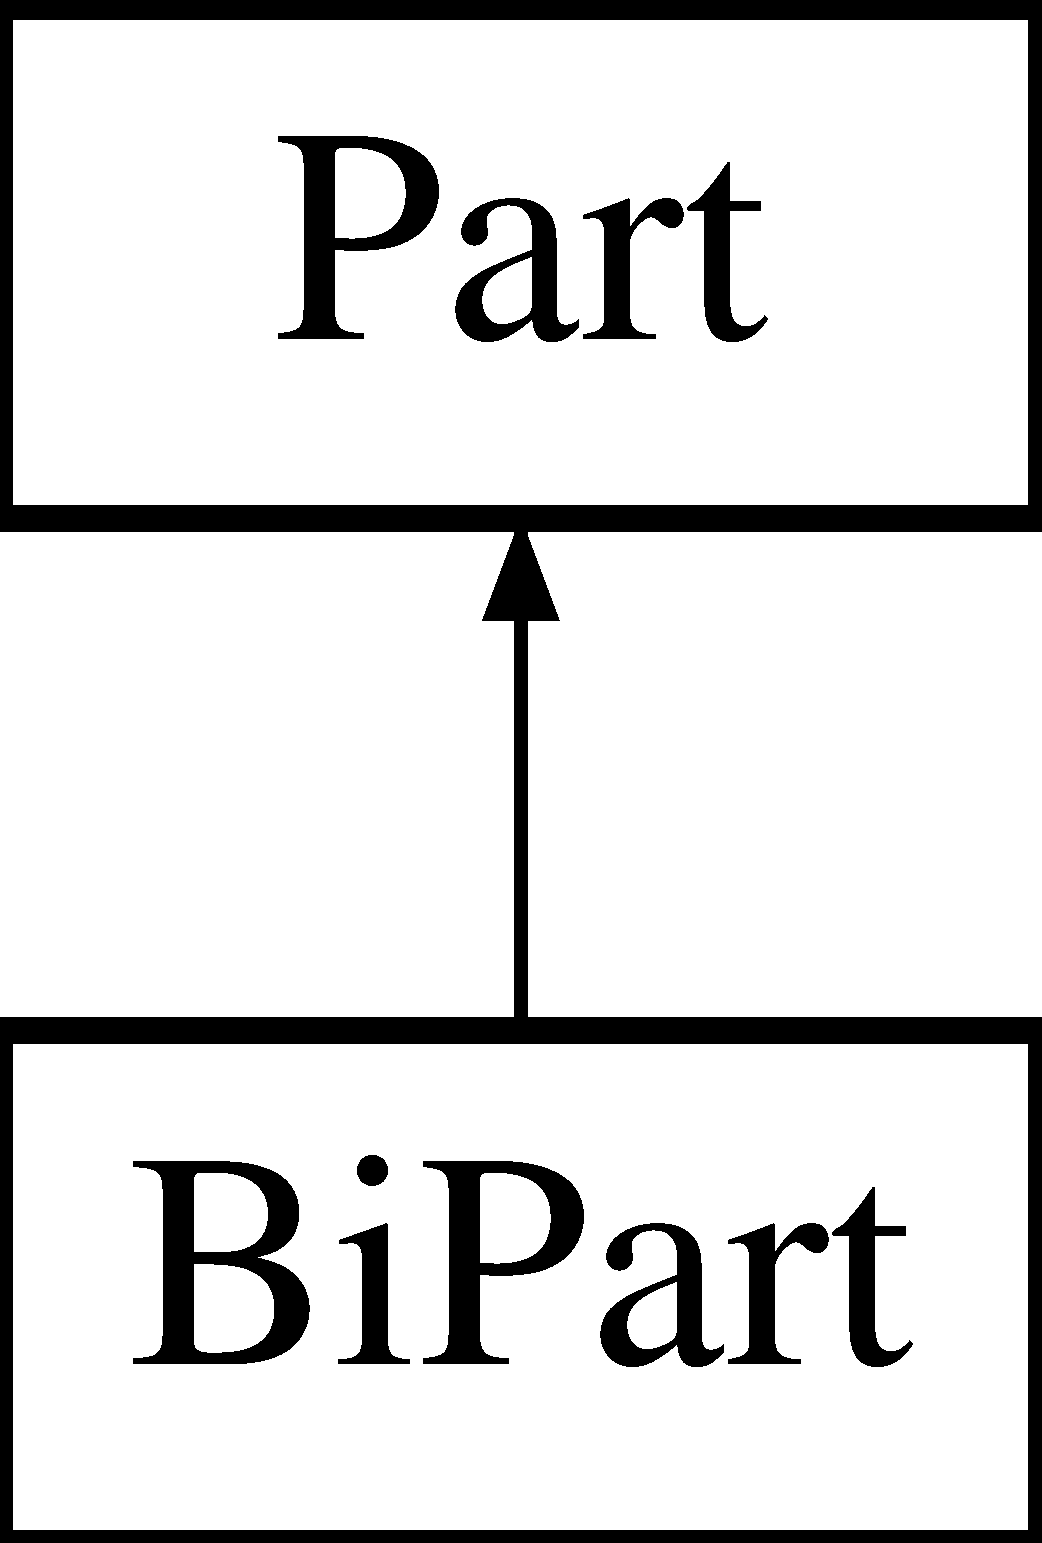
\includegraphics[height=2.000000cm]{classBiPart}
\end{center}
\end{figure}
\subsection*{Public Member Functions}
\begin{DoxyCompactItemize}
\item 
\hypertarget{classBiPart_aa3d9446a9207461c5b9ec328c3ef61ae}{{\bfseries Bi\-Part} (\hyperlink{classPart}{Part} $\ast$part1, \hyperlink{classPart}{Part} $\ast$part2, \hyperlink{classObjectiveValue}{Objective\-Value} $\ast$value=0)}\label{classBiPart_aa3d9446a9207461c5b9ec328c3ef61ae}

\item 
\hypertarget{classBiPart_ae80858643535d37f3cc96f0fccc947ff}{{\bfseries Bi\-Part} (\hyperlink{classBiPart}{Bi\-Part} $\ast$bi\-Part)}\label{classBiPart_ae80858643535d37f3cc96f0fccc947ff}

\item 
\hypertarget{classBiPart_a242f8d88da324a08bd296ea69cd7360f}{bool {\bfseries equal} (\hyperlink{classPart}{Part} $\ast$p)}\label{classBiPart_a242f8d88da324a08bd296ea69cd7360f}

\item 
\hypertarget{classBiPart_a2fb0a97551bcfc4a9bda5fa1307703d6}{void {\bfseries print} (bool endl=false)}\label{classBiPart_a2fb0a97551bcfc4a9bda5fa1307703d6}

\item 
\hypertarget{classBiPart_aace53eab6f4e8b2f676c0ed7d8f6c9b5}{int {\bfseries print\-Size} ()}\label{classBiPart_aace53eab6f4e8b2f676c0ed7d8f6c9b5}

\end{DoxyCompactItemize}
\subsection*{Public Attributes}
\begin{DoxyCompactItemize}
\item 
\hypertarget{classBiPart_a5846464cf88602318aa6c4f26976255b}{\hyperlink{classPart}{Part} $\ast$ {\bfseries first\-Part}}\label{classBiPart_a5846464cf88602318aa6c4f26976255b}

\item 
\hypertarget{classBiPart_a3497ede9e6226b6b71b39e481d07c63e}{\hyperlink{classPart}{Part} $\ast$ {\bfseries second\-Part}}\label{classBiPart_a3497ede9e6226b6b71b39e481d07c63e}

\end{DoxyCompactItemize}


The documentation for this class was generated from the following files\-:\begin{DoxyCompactItemize}
\item 
/home/lamarche/programming/optimal\-\_\-partition/src/partition.\-hpp\item 
/home/lamarche/programming/optimal\-\_\-partition/src/partition.\-cpp\end{DoxyCompactItemize}

\hypertarget{classBiSet}{\section{Bi\-Set Class Reference}
\label{classBiSet}\index{Bi\-Set@{Bi\-Set}}
}
Inheritance diagram for Bi\-Set\-:\begin{figure}[H]
\begin{center}
\leavevmode
\includegraphics[height=2.000000cm]{classBiSet}
\end{center}
\end{figure}
\subsection*{Public Member Functions}
\begin{DoxyCompactItemize}
\item 
\hypertarget{classBiSet_afe9de2b49fc94e52d01b6b48175393dd}{{\bfseries Bi\-Set} (\hyperlink{classUniSet}{Uni\-Set} $\ast$uni\-Set1, \hyperlink{classUniSet}{Uni\-Set} $\ast$uni\-Set2)}\label{classBiSet_afe9de2b49fc94e52d01b6b48175393dd}

\item 
\hypertarget{classBiSet_adf57958f51107b7ce2af16d72a1f872b}{void {\bfseries init\-Reached} ()}\label{classBiSet_adf57958f51107b7ce2af16d72a1f872b}

\item 
\hypertarget{classBiSet_addab16bb60c987ae2f08f23dbbc30864}{void \hyperlink{classBiSet_addab16bb60c987ae2f08f23dbbc30864}{set\-Random} ()}\label{classBiSet_addab16bb60c987ae2f08f23dbbc30864}

\begin{DoxyCompactList}\small\item\em Randomly set the algebraic constraints for quick experiments (warning\-: this method is not always implemented) \end{DoxyCompactList}\item 
void \hyperlink{classBiSet_aa81de5cee7bae0c86493b31ceb5199b8}{set\-Objective\-Function} (\hyperlink{classObjectiveFunction}{Objective\-Function} $\ast$m)
\begin{DoxyCompactList}\small\item\em Set the objective that one wants to optimise. \end{DoxyCompactList}\item 
\hypertarget{classBiSet_aec73ba21855b517d003d3c02b14fbcec}{void \hyperlink{classBiSet_aec73ba21855b517d003d3c02b14fbcec}{print} ()}\label{classBiSet_aec73ba21855b517d003d3c02b14fbcec}

\begin{DoxyCompactList}\small\item\em Print the set and its algebraic constraints. \end{DoxyCompactList}\item 
\hypertarget{classBiSet_a4be98bd081fec38aeaaa630c358fcac2}{void \hyperlink{classBiSet_a4be98bd081fec38aeaaa630c358fcac2}{build\-Data\-Structure} ()}\label{classBiSet_a4be98bd081fec38aeaaa630c358fcac2}

\begin{DoxyCompactList}\small\item\em Build a proper data structure to represent the set and its algebraic constraints (warning\-: this method should always be called after instantiating and parameterising a set, and before calling any other method, such as \hyperlink{classBiSet_aec73ba21855b517d003d3c02b14fbcec}{print()}, \hyperlink{classBiSet_ad2ee8efa76c2d023d60cb8d203b4b365}{compute\-Objective\-Values()}, compute\-Optimal\-Partition (double parameter), etc.) \end{DoxyCompactList}\item 
\hypertarget{classBiSet_ad2ee8efa76c2d023d60cb8d203b4b365}{void \hyperlink{classBiSet_ad2ee8efa76c2d023d60cb8d203b4b365}{compute\-Objective\-Values} ()}\label{classBiSet_ad2ee8efa76c2d023d60cb8d203b4b365}

\begin{DoxyCompactList}\small\item\em Compute the value of the objective function for each feasible part (warning\-: set\-Objective\-Function (\hyperlink{classObjectiveFunction}{Objective\-Function} $\ast$objective) should have been called first) \end{DoxyCompactList}\item 
\hypertarget{classBiSet_ae630d13ca1803d3c0d0422f839d8806a}{void \hyperlink{classBiSet_ae630d13ca1803d3c0d0422f839d8806a}{normalize\-Objective\-Values} ()}\label{classBiSet_ae630d13ca1803d3c0d0422f839d8806a}

\begin{DoxyCompactList}\small\item\em Finish computing the value of the objective function for each feasible part when normalisation is required (warning\-: only after \hyperlink{classBiSet_ad2ee8efa76c2d023d60cb8d203b4b365}{compute\-Objective\-Values()} has been called) \end{DoxyCompactList}\item 
\hypertarget{classBiSet_aabdac7b50292f744157c3ffd0b37f648}{void \hyperlink{classBiSet_aabdac7b50292f744157c3ffd0b37f648}{print\-Objective\-Values} ()}\label{classBiSet_aabdac7b50292f744157c3ffd0b37f648}

\begin{DoxyCompactList}\small\item\em Print the value of the objective function for each feasible part. \end{DoxyCompactList}\item 
void \hyperlink{classBiSet_a1604b2e1d322552fe83e5e2933ac2bd3}{compute\-Optimal\-Partition} (double parameter)
\begin{DoxyCompactList}\small\item\em Compute a partition that fits with the algebraic constraints and that optimises the objective function that has been specified. \end{DoxyCompactList}\item 
void \hyperlink{classBiSet_ad8abd03c606bb3e3bdac6037c1b955a6}{print\-Optimal\-Partition} (double parameter)
\begin{DoxyCompactList}\small\item\em Compute and print a partition that fits with the algebraic constraints and that optimises the objective function that has been specified (warning\-: this method is not always implemented, but one can obtain a similar result by using get\-Optimal\-Partition (double parameter) and by calling \hyperlink{classBiSet_aec73ba21855b517d003d3c02b14fbcec}{print()} on the result) \end{DoxyCompactList}\item 
\hyperlink{classPartition}{Partition} $\ast$ \hyperlink{classBiSet_a5f79a8811a0638bcfc418c100b4f67af}{get\-Optimal\-Partition} (double parameter)
\begin{DoxyCompactList}\small\item\em Compute and return a partition that fits with the algebraic constraints and that optimises the objective function that has been specified (warning\-: this method is not always implemented, but one can obtain a similar result by using get\-Optimal\-Partition (double parameter) and by calling \hyperlink{classBiSet_aec73ba21855b517d003d3c02b14fbcec}{print()} on the result) \end{DoxyCompactList}\end{DoxyCompactItemize}
\subsection*{Public Attributes}
\begin{DoxyCompactItemize}
\item 
\hypertarget{classBiSet_abd13f5daf7fdc2851463c493e0a3abbb}{\hyperlink{classUniSet}{Uni\-Set} $\ast$ {\bfseries uni\-Set1}}\label{classBiSet_abd13f5daf7fdc2851463c493e0a3abbb}

\item 
\hypertarget{classBiSet_a094429b1556bda1cdf62a2d9372980db}{\hyperlink{classUniSet}{Uni\-Set} $\ast$ {\bfseries uni\-Set2}}\label{classBiSet_a094429b1556bda1cdf62a2d9372980db}

\item 
\hypertarget{classBiSet_af7577011b1a03a83a822300d8f1dacc6}{int {\bfseries bi\-Subset\-Number}}\label{classBiSet_af7577011b1a03a83a822300d8f1dacc6}

\item 
\hypertarget{classBiSet_a2d2c420ff44d5e1f022c7459b902fd0c}{int {\bfseries atomic\-Bi\-Subset\-Number}}\label{classBiSet_a2d2c420ff44d5e1f022c7459b902fd0c}

\item 
\hypertarget{classBiSet_a1c5df2c47b9a34e0870836e199fba6a0}{\hyperlink{classBiSubset}{Bi\-Subset} $\ast$ {\bfseries first\-Bi\-Subset}}\label{classBiSet_a1c5df2c47b9a34e0870836e199fba6a0}

\item 
\hypertarget{classBiSet_a67c530d5795d293b94a57cfa4cc35461}{\hyperlink{classBiSubset}{Bi\-Subset} $\ast$$\ast$ {\bfseries bi\-Subset\-Array}}\label{classBiSet_a67c530d5795d293b94a57cfa4cc35461}

\end{DoxyCompactItemize}


\subsection{Member Function Documentation}
\hypertarget{classBiSet_a1604b2e1d322552fe83e5e2933ac2bd3}{\index{Bi\-Set@{Bi\-Set}!compute\-Optimal\-Partition@{compute\-Optimal\-Partition}}
\index{compute\-Optimal\-Partition@{compute\-Optimal\-Partition}!BiSet@{Bi\-Set}}
\subsubsection[{compute\-Optimal\-Partition}]{\setlength{\rightskip}{0pt plus 5cm}void Bi\-Set\-::compute\-Optimal\-Partition (
\begin{DoxyParamCaption}
\item[{double}]{parameter}
\end{DoxyParamCaption}
)\hspace{0.3cm}{\ttfamily [virtual]}}}\label{classBiSet_a1604b2e1d322552fe83e5e2933ac2bd3}


Compute a partition that fits with the algebraic constraints and that optimises the objective function that has been specified. 


\begin{DoxyParams}{Parameters}
{\em parameter} & \-: The parameter of the objective function to be optimised (if the objective is parametrised) \\
\hline
\end{DoxyParams}


Implements \hyperlink{classAbstractSet_acfc3004f18192f38e32bb7a5a12ec8df}{Abstract\-Set}.

\hypertarget{classBiSet_a5f79a8811a0638bcfc418c100b4f67af}{\index{Bi\-Set@{Bi\-Set}!get\-Optimal\-Partition@{get\-Optimal\-Partition}}
\index{get\-Optimal\-Partition@{get\-Optimal\-Partition}!BiSet@{Bi\-Set}}
\subsubsection[{get\-Optimal\-Partition}]{\setlength{\rightskip}{0pt plus 5cm}{\bf Partition} $\ast$ Bi\-Set\-::get\-Optimal\-Partition (
\begin{DoxyParamCaption}
\item[{double}]{parameter}
\end{DoxyParamCaption}
)\hspace{0.3cm}{\ttfamily [virtual]}}}\label{classBiSet_a5f79a8811a0638bcfc418c100b4f67af}


Compute and return a partition that fits with the algebraic constraints and that optimises the objective function that has been specified (warning\-: this method is not always implemented, but one can obtain a similar result by using get\-Optimal\-Partition (double parameter) and by calling \hyperlink{classBiSet_aec73ba21855b517d003d3c02b14fbcec}{print()} on the result) 


\begin{DoxyParams}{Parameters}
{\em parameter} & \-: The parameter of the objective function to be optimised (if the objective is parametrised) \\
\hline
\end{DoxyParams}
\begin{DoxyReturn}{Returns}
\-: The resulting optimal partition 
\end{DoxyReturn}


Implements \hyperlink{classAbstractSet_a48fd08c4b61ed46946bed6e19cd11194}{Abstract\-Set}.

\hypertarget{classBiSet_ad8abd03c606bb3e3bdac6037c1b955a6}{\index{Bi\-Set@{Bi\-Set}!print\-Optimal\-Partition@{print\-Optimal\-Partition}}
\index{print\-Optimal\-Partition@{print\-Optimal\-Partition}!BiSet@{Bi\-Set}}
\subsubsection[{print\-Optimal\-Partition}]{\setlength{\rightskip}{0pt plus 5cm}void Bi\-Set\-::print\-Optimal\-Partition (
\begin{DoxyParamCaption}
\item[{double}]{parameter}
\end{DoxyParamCaption}
)\hspace{0.3cm}{\ttfamily [virtual]}}}\label{classBiSet_ad8abd03c606bb3e3bdac6037c1b955a6}


Compute and print a partition that fits with the algebraic constraints and that optimises the objective function that has been specified (warning\-: this method is not always implemented, but one can obtain a similar result by using get\-Optimal\-Partition (double parameter) and by calling \hyperlink{classBiSet_aec73ba21855b517d003d3c02b14fbcec}{print()} on the result) 


\begin{DoxyParams}{Parameters}
{\em parameter} & \-: The parameter of the objective function to be optimised (if the objective is parametrised) \\
\hline
\end{DoxyParams}


Implements \hyperlink{classAbstractSet_a82a9ce5c2d30690f0d1b83b034e92e1e}{Abstract\-Set}.

\hypertarget{classBiSet_aa81de5cee7bae0c86493b31ceb5199b8}{\index{Bi\-Set@{Bi\-Set}!set\-Objective\-Function@{set\-Objective\-Function}}
\index{set\-Objective\-Function@{set\-Objective\-Function}!BiSet@{Bi\-Set}}
\subsubsection[{set\-Objective\-Function}]{\setlength{\rightskip}{0pt plus 5cm}void Bi\-Set\-::set\-Objective\-Function (
\begin{DoxyParamCaption}
\item[{{\bf Objective\-Function} $\ast$}]{objective}
\end{DoxyParamCaption}
)\hspace{0.3cm}{\ttfamily [virtual]}}}\label{classBiSet_aa81de5cee7bae0c86493b31ceb5199b8}


Set the objective that one wants to optimise. 


\begin{DoxyParams}{Parameters}
{\em objective} & \-: The objective function itself \\
\hline
\end{DoxyParams}


Implements \hyperlink{classAbstractSet_a7aef71679a18ab7965d1098da15b26c2}{Abstract\-Set}.



The documentation for this class was generated from the following files\-:\begin{DoxyCompactItemize}
\item 
src/bi\-\_\-set.\-hpp\item 
src/bi\-\_\-set.\-cpp\end{DoxyCompactItemize}

\hypertarget{classBiSubset}{\section{Bi\-Subset Class Reference}
\label{classBiSubset}\index{Bi\-Subset@{Bi\-Subset}}
}
\subsection*{Public Member Functions}
\begin{DoxyCompactItemize}
\item 
\hypertarget{classBiSubset_a72dab80dd500f97f37b85978fcd0e215}{{\bfseries Bi\-Subset} (\hyperlink{classUniSubset}{Uni\-Subset} $\ast$uni\-Subset1, \hyperlink{classUniSubset}{Uni\-Subset} $\ast$uni\-Subset2)}\label{classBiSubset_a72dab80dd500f97f37b85978fcd0e215}

\item 
\hypertarget{classBiSubset_a9e2244b5abe28961262331d4552f349b}{void {\bfseries print} ()}\label{classBiSubset_a9e2244b5abe28961262331d4552f349b}

\item 
\hypertarget{classBiSubset_abd1cc08db6ce34f7ac8a25ca2d752561}{void {\bfseries print\-Index\-Set} (bool endl=false)}\label{classBiSubset_abd1cc08db6ce34f7ac8a25ca2d752561}

\item 
\hypertarget{classBiSubset_aeb28fe63a6de896ca68ac0729febd553}{void {\bfseries add\-Bi\-Subset\-Set} (Bi\-Subset\-Set $\ast$bi\-Subset\-Set)}\label{classBiSubset_aeb28fe63a6de896ca68ac0729febd553}

\item 
\hypertarget{classBiSubset_a4ac853c296b879fc071568aa86c9b2b7}{void {\bfseries set\-Objective\-Function} (\hyperlink{classObjectiveFunction}{Objective\-Function} $\ast$m)}\label{classBiSubset_a4ac853c296b879fc071568aa86c9b2b7}

\item 
\hypertarget{classBiSubset_ac78205261912722ccae75e1ca8c8ff68}{void {\bfseries build\-Data\-Structure} ()}\label{classBiSubset_ac78205261912722ccae75e1ca8c8ff68}

\item 
\hypertarget{classBiSubset_ac815043eae3451a4aacc76e7324dd445}{void {\bfseries compute\-Objective\-Values} ()}\label{classBiSubset_ac815043eae3451a4aacc76e7324dd445}

\item 
\hypertarget{classBiSubset_a9671b38670ed6a9e25cb2afaf606a4ee}{void {\bfseries normalize\-Objective\-Values} (\hyperlink{classObjectiveValue}{Objective\-Value} $\ast$max\-Qual=0)}\label{classBiSubset_a9671b38670ed6a9e25cb2afaf606a4ee}

\item 
\hypertarget{classBiSubset_a8bcaee7528bdd231cc945dd429979a01}{void {\bfseries print\-Objective\-Values} ()}\label{classBiSubset_a8bcaee7528bdd231cc945dd429979a01}

\item 
\hypertarget{classBiSubset_aabba7f3c7e8371a78b9ddce159a1624f}{void {\bfseries compute\-Optimal\-Partition} (double parameter)}\label{classBiSubset_aabba7f3c7e8371a78b9ddce159a1624f}

\item 
\hypertarget{classBiSubset_a82c0cbc273a32a52a9ac98db3506dfd3}{void {\bfseries print\-Optimal\-Partition} (double parameter)}\label{classBiSubset_a82c0cbc273a32a52a9ac98db3506dfd3}

\item 
\hypertarget{classBiSubset_aafc0f7b74dcb498779cef5b6a9385e30}{void {\bfseries build\-Optimal\-Partition} (\hyperlink{classPartition}{Partition} $\ast$partition)}\label{classBiSubset_aafc0f7b74dcb498779cef5b6a9385e30}

\end{DoxyCompactItemize}
\subsection*{Public Attributes}
\begin{DoxyCompactItemize}
\item 
\hypertarget{classBiSubset_a77f74c22c4aa92f91bd78308b2226722}{\hyperlink{classUniSubset}{Uni\-Subset} $\ast$ {\bfseries uni\-Subset1}}\label{classBiSubset_a77f74c22c4aa92f91bd78308b2226722}

\item 
\hypertarget{classBiSubset_ac457d4d17b160513bdbb0ebd0e953e98}{\hyperlink{classUniSubset}{Uni\-Subset} $\ast$ {\bfseries uni\-Subset2}}\label{classBiSubset_ac457d4d17b160513bdbb0ebd0e953e98}

\item 
\hypertarget{classBiSubset_a2c5e87f3e494ab45378f4a164067b593}{int {\bfseries num}}\label{classBiSubset_a2c5e87f3e494ab45378f4a164067b593}

\item 
\hypertarget{classBiSubset_ab99e33ac14000f58d9857ed350b22945}{bool {\bfseries is\-Atomic}}\label{classBiSubset_ab99e33ac14000f58d9857ed350b22945}

\item 
\hypertarget{classBiSubset_a62f9d6c80da8a1c1042cf7fc62c2fd74}{bool {\bfseries reached}}\label{classBiSubset_a62f9d6c80da8a1c1042cf7fc62c2fd74}

\item 
\hypertarget{classBiSubset_ae7762449606cb0881912516b860c02af}{Bi\-Subset\-Set\-Set $\ast$ {\bfseries bi\-Subset\-Set\-Set}}\label{classBiSubset_ae7762449606cb0881912516b860c02af}

\item 
\hypertarget{classBiSubset_a1032827bad10a9ecca017392a748b7fa}{\hyperlink{classBiSet}{Bi\-Set} $\ast$ {\bfseries bi\-Set}}\label{classBiSubset_a1032827bad10a9ecca017392a748b7fa}

\item 
\hypertarget{classBiSubset_a7ef49d4b3b6d7af08a01602a0edf34b8}{\hyperlink{classObjectiveFunction}{Objective\-Function} $\ast$ {\bfseries objective}}\label{classBiSubset_a7ef49d4b3b6d7af08a01602a0edf34b8}

\item 
\hypertarget{classBiSubset_a9db1dc5225f9f61d579dbef600d567b8}{\hyperlink{classObjectiveValue}{Objective\-Value} $\ast$ {\bfseries value}}\label{classBiSubset_a9db1dc5225f9f61d579dbef600d567b8}

\item 
\hypertarget{classBiSubset_adf8bd52488fe0c1aae0b6c32a6dac812}{double {\bfseries optimal\-Value}}\label{classBiSubset_adf8bd52488fe0c1aae0b6c32a6dac812}

\item 
\hypertarget{classBiSubset_a0cd31189cc46810f4c753ab12ebb4d47}{Bi\-Subset\-Set $\ast$ {\bfseries optimal\-Cut}}\label{classBiSubset_a0cd31189cc46810f4c753ab12ebb4d47}

\end{DoxyCompactItemize}


The documentation for this class was generated from the following files\-:\begin{DoxyCompactItemize}
\item 
src/bi\-\_\-set.\-hpp\item 
src/bi\-\_\-set.\-cpp\end{DoxyCompactItemize}

\hypertarget{classBottleneckObjectiveValue}{\section{Bottleneck\-Objective\-Value Class Reference}
\label{classBottleneckObjectiveValue}\index{Bottleneck\-Objective\-Value@{Bottleneck\-Objective\-Value}}
}
Inheritance diagram for Bottleneck\-Objective\-Value\-:\begin{figure}[H]
\begin{center}
\leavevmode
\includegraphics[height=2.000000cm]{classBottleneckObjectiveValue}
\end{center}
\end{figure}
\subsection*{Public Member Functions}
\begin{DoxyCompactItemize}
\item 
\hypertarget{classBottleneckObjectiveValue_a472c19dd35594975cdc8d63b06bec066}{{\bfseries Bottleneck\-Objective\-Value} (\hyperlink{classInformationBottleneck}{Information\-Bottleneck} $\ast$objective, int index=-\/1)}\label{classBottleneckObjectiveValue_a472c19dd35594975cdc8d63b06bec066}

\item 
\hypertarget{classBottleneckObjectiveValue_acca02ede3d42cbb71852339087bdff22}{void {\bfseries add} (\hyperlink{classObjectiveValue}{Objective\-Value} $\ast$value)}\label{classBottleneckObjectiveValue_acca02ede3d42cbb71852339087bdff22}

\item 
\hypertarget{classBottleneckObjectiveValue_a2a1bfd06ae2ae78f7e347703f1805984}{void {\bfseries compute} ()}\label{classBottleneckObjectiveValue_a2a1bfd06ae2ae78f7e347703f1805984}

\item 
\hypertarget{classBottleneckObjectiveValue_ac6672e91013a5667488e7fccbc452fed}{void {\bfseries compute} (\hyperlink{classObjectiveValue}{Objective\-Value} $\ast$value1, \hyperlink{classObjectiveValue}{Objective\-Value} $\ast$value2)}\label{classBottleneckObjectiveValue_ac6672e91013a5667488e7fccbc452fed}

\item 
\hypertarget{classBottleneckObjectiveValue_ae6edb61731a33a8c3c28c9de3f011fa9}{void {\bfseries compute} (Objective\-Value\-Set $\ast$value\-Set)}\label{classBottleneckObjectiveValue_ae6edb61731a33a8c3c28c9de3f011fa9}

\item 
\hypertarget{classBottleneckObjectiveValue_a20cd5a3dce433043a3ce9641fc6df8b3}{void {\bfseries normalize} (\hyperlink{classObjectiveValue}{Objective\-Value} $\ast$q)}\label{classBottleneckObjectiveValue_a20cd5a3dce433043a3ce9641fc6df8b3}

\item 
\hypertarget{classBottleneckObjectiveValue_a5dd538d1531ca10fc8b1261ee83be8f2}{void {\bfseries print} (bool verbose=true)}\label{classBottleneckObjectiveValue_a5dd538d1531ca10fc8b1261ee83be8f2}

\item 
\hypertarget{classBottleneckObjectiveValue_a76d0963588415208aca8da0d1f1b4600}{double {\bfseries get\-Value} (double param)}\label{classBottleneckObjectiveValue_a76d0963588415208aca8da0d1f1b4600}

\end{DoxyCompactItemize}
\subsection*{Public Attributes}
\begin{DoxyCompactItemize}
\item 
\hypertarget{classBottleneckObjectiveValue_a6229987020b8634ca238bb7d6d8904db}{int {\bfseries index}}\label{classBottleneckObjectiveValue_a6229987020b8634ca238bb7d6d8904db}

\item 
\hypertarget{classBottleneckObjectiveValue_a0e9546f57c845f33372ac3db29f8ea25}{double {\bfseries pk}}\label{classBottleneckObjectiveValue_a0e9546f57c845f33372ac3db29f8ea25}

\item 
\hypertarget{classBottleneckObjectiveValue_ac823f5e398f9ae9c75fe9151b29aac5b}{double $\ast$ {\bfseries pkj}}\label{classBottleneckObjectiveValue_ac823f5e398f9ae9c75fe9151b29aac5b}

\item 
\hypertarget{classBottleneckObjectiveValue_ac6c6fa26dac3f438159c5c7c6f1b4f3b}{double $\ast$ {\bfseries pj}}\label{classBottleneckObjectiveValue_ac6c6fa26dac3f438159c5c7c6f1b4f3b}

\item 
\hypertarget{classBottleneckObjectiveValue_a227ccad30a07de0b38e4678940b06338}{double {\bfseries Iki}}\label{classBottleneckObjectiveValue_a227ccad30a07de0b38e4678940b06338}

\item 
\hypertarget{classBottleneckObjectiveValue_a40c60ab77263afa0738968433d2d425f}{double {\bfseries Ikj}}\label{classBottleneckObjectiveValue_a40c60ab77263afa0738968433d2d425f}

\end{DoxyCompactItemize}


The documentation for this class was generated from the following files\-:\begin{DoxyCompactItemize}
\item 
/home/lamarche/programming/optimal\-\_\-partition/src/information\-\_\-bottleneck.\-hpp\item 
/home/lamarche/programming/optimal\-\_\-partition/src/information\-\_\-bottleneck.\-cpp\end{DoxyCompactItemize}

\hypertarget{classChainVoterGraph}{\section{Chain\-Voter\-Graph Class Reference}
\label{classChainVoterGraph}\index{Chain\-Voter\-Graph@{Chain\-Voter\-Graph}}
}
Inheritance diagram for Chain\-Voter\-Graph\-:\begin{figure}[H]
\begin{center}
\leavevmode
\includegraphics[height=2.000000cm]{classChainVoterGraph}
\end{center}
\end{figure}
\subsection*{Public Member Functions}
\begin{DoxyCompactItemize}
\item 
\hypertarget{classChainVoterGraph_af0e0e5327d26e67d46df0b33bb009c69}{{\bfseries Chain\-Voter\-Graph} (int size, double contrarian=0, bool ring=false, int update=\hyperlink{voter__graph_8hpp_ab3bec55c359e4ed771339c8bc61fc35aa01d100088352e1a7d3a34c9a66d0f951}{U\-P\-D\-A\-T\-E\-\_\-\-E\-D\-G\-E\-S})}\label{classChainVoterGraph_af0e0e5327d26e67d46df0b33bb009c69}

\end{DoxyCompactItemize}
\subsection*{Public Attributes}
\begin{DoxyCompactItemize}
\item 
\hypertarget{classChainVoterGraph_a03a3e2fb44bd8c4e0e1697545d4eff65}{int {\bfseries size}}\label{classChainVoterGraph_a03a3e2fb44bd8c4e0e1697545d4eff65}

\item 
\hypertarget{classChainVoterGraph_ace4b3a77876d38f216552e4b5bfaf32b}{double {\bfseries contrarian}}\label{classChainVoterGraph_ace4b3a77876d38f216552e4b5bfaf32b}

\item 
\hypertarget{classChainVoterGraph_a0b9e76e99e2666ca7e92ec757ce24d32}{\hyperlink{classVoterNode}{Voter\-Node} $\ast$$\ast$ {\bfseries node\-Array}}\label{classChainVoterGraph_a0b9e76e99e2666ca7e92ec757ce24d32}

\item 
\hypertarget{classChainVoterGraph_afb107128956fbedd499dfbfeef8fe14c}{bool {\bfseries ring}}\label{classChainVoterGraph_afb107128956fbedd499dfbfeef8fe14c}

\end{DoxyCompactItemize}


The documentation for this class was generated from the following files\-:\begin{DoxyCompactItemize}
\item 
src/\hyperlink{voter__graph_8hpp}{voter\-\_\-graph.\-hpp}\item 
src/voter\-\_\-graph.\-cpp\end{DoxyCompactItemize}

\hypertarget{classCompleteGraph}{\section{Complete\-Graph Class Reference}
\label{classCompleteGraph}\index{Complete\-Graph@{Complete\-Graph}}
}
Inheritance diagram for Complete\-Graph\-:\begin{figure}[H]
\begin{center}
\leavevmode
\includegraphics[height=3.000000cm]{classCompleteGraph}
\end{center}
\end{figure}
\subsection*{Public Member Functions}
\begin{DoxyCompactItemize}
\item 
\hypertarget{classCompleteGraph_ab74d38ce74de8bd6e413d416af89d9fa}{{\bfseries Complete\-Graph} (int v\-Num)}\label{classCompleteGraph_ab74d38ce74de8bd6e413d416af89d9fa}

\end{DoxyCompactItemize}
\subsection*{Additional Inherited Members}


The documentation for this class was generated from the following file\-:\begin{DoxyCompactItemize}
\item 
/home/lamarche/programming/optimal\-\_\-partition/src/graph.\-hpp\end{DoxyCompactItemize}

\hypertarget{classCompleteVoterGraph}{\section{Complete\-Voter\-Graph Class Reference}
\label{classCompleteVoterGraph}\index{Complete\-Voter\-Graph@{Complete\-Voter\-Graph}}
}


An interaction graph with edges between each pair of nodes (in both direction, with equal weight for each edge)  




{\ttfamily \#include $<$voter\-\_\-graph.\-hpp$>$}

Inheritance diagram for Complete\-Voter\-Graph\-:\begin{figure}[H]
\begin{center}
\leavevmode
\includegraphics[height=2.000000cm]{classCompleteVoterGraph}
\end{center}
\end{figure}
\subsection*{Public Member Functions}
\begin{DoxyCompactItemize}
\item 
\hyperlink{classCompleteVoterGraph_a0adf42ee4826aa54e1a13d9b8d770554}{Complete\-Voter\-Graph} (int size, int update=\hyperlink{voter__graph_8hpp_ab3bec55c359e4ed771339c8bc61fc35aa01d100088352e1a7d3a34c9a66d0f951}{U\-P\-D\-A\-T\-E\-\_\-\-E\-D\-G\-E\-S}, double contrarian=0)
\begin{DoxyCompactList}\small\item\em Constructor. \end{DoxyCompactList}\end{DoxyCompactItemize}
\subsection*{Additional Inherited Members}


\subsection{Detailed Description}
An interaction graph with edges between each pair of nodes (in both direction, with equal weight for each edge) 

\subsection{Constructor \& Destructor Documentation}
\hypertarget{classCompleteVoterGraph_a0adf42ee4826aa54e1a13d9b8d770554}{\index{Complete\-Voter\-Graph@{Complete\-Voter\-Graph}!Complete\-Voter\-Graph@{Complete\-Voter\-Graph}}
\index{Complete\-Voter\-Graph@{Complete\-Voter\-Graph}!CompleteVoterGraph@{Complete\-Voter\-Graph}}
\subsubsection[{Complete\-Voter\-Graph}]{\setlength{\rightskip}{0pt plus 5cm}Complete\-Voter\-Graph\-::\-Complete\-Voter\-Graph (
\begin{DoxyParamCaption}
\item[{int}]{size, }
\item[{int}]{update = {\ttfamily {\bf U\-P\-D\-A\-T\-E\-\_\-\-E\-D\-G\-E\-S}}, }
\item[{double}]{contrarian = {\ttfamily 0}}
\end{DoxyParamCaption}
)}}\label{classCompleteVoterGraph_a0adf42ee4826aa54e1a13d9b8d770554}


Constructor. 


\begin{DoxyParams}{Parameters}
{\em size} & \-: Size of the graph \\
\hline
{\em update} & \-: How the system evolves at each simulation step (U\-P\-D\-A\-T\-E\-\_\-\-N\-O\-D\-E\-S or U\-P\-D\-A\-T\-E\-\_\-\-E\-D\-G\-E\-S) \\
\hline
{\em contrarian} & \-: The contrarian rate of each node \\
\hline
\end{DoxyParams}


The documentation for this class was generated from the following files\-:\begin{DoxyCompactItemize}
\item 
src/\hyperlink{voter__graph_8hpp}{voter\-\_\-graph.\-hpp}\item 
src/voter\-\_\-graph.\-cpp\end{DoxyCompactItemize}

\hypertarget{structDataPointStruct}{\section{Data\-Point\-Struct Struct Reference}
\label{structDataPointStruct}\index{Data\-Point\-Struct@{Data\-Point\-Struct}}
}
\subsection*{Public Attributes}
\begin{DoxyCompactItemize}
\item 
\hypertarget{structDataPointStruct_ab19cdad849d37de06c02cacc5ec50cce}{std\-::vector$<$ int $>$ {\bfseries parameters}}\label{structDataPointStruct_ab19cdad849d37de06c02cacc5ec50cce}

\item 
\hypertarget{structDataPointStruct_ae1dae54ff363ef8a6d946907b1621506}{float {\bfseries time}}\label{structDataPointStruct_ae1dae54ff363ef8a6d946907b1621506}

\item 
\hypertarget{structDataPointStruct_a6d345b8aa7e79cd06402446d73d19520}{int {\bfseries memory}}\label{structDataPointStruct_a6d345b8aa7e79cd06402446d73d19520}

\end{DoxyCompactItemize}


The documentation for this struct was generated from the following file\-:\begin{DoxyCompactItemize}
\item 
/home/lamarche/programming/optimal\-\_\-partition/src/timer.\-hpp\end{DoxyCompactItemize}

\hypertarget{classDataset}{\section{Dataset Class Reference}
\label{classDataset}\index{Dataset@{Dataset}}
}
\subsection*{Public Member Functions}
\begin{DoxyCompactItemize}
\item 
\hypertarget{classDataset_a8feaf2bb311910ab4d99d2e4bf1463b9}{void {\bfseries print} ()}\label{classDataset_a8feaf2bb311910ab4d99d2e4bf1463b9}

\item 
\hypertarget{classDataset_ac60d60df61e67a22b131642ab4dd06d4}{void {\bfseries build\-Dataset} ()}\label{classDataset_ac60d60df61e67a22b131642ab4dd06d4}

\item 
\hypertarget{classDataset_a9a50f1d277ee5fbd065e5e99ebe5b40b}{void {\bfseries init\-Values} (double v=0)}\label{classDataset_a9a50f1d277ee5fbd065e5e99ebe5b40b}

\item 
\hypertarget{classDataset_a6ac9666627e5f9d96660faff51b8bd8d}{void {\bfseries init\-Ref\-Values} (double v=0)}\label{classDataset_a6ac9666627e5f9d96660faff51b8bd8d}

\item 
\hypertarget{classDataset_a4b062bc0218c18b32e266d02b67ee8dd}{void {\bfseries add\-Label1} (std\-::string str)}\label{classDataset_a4b062bc0218c18b32e266d02b67ee8dd}

\item 
\hypertarget{classDataset_a7c4c161be1a352682d64a7a829366f4a}{void {\bfseries add\-Label2} (std\-::string str)}\label{classDataset_a7c4c161be1a352682d64a7a829366f4a}

\item 
\hypertarget{classDataset_a9a3da37b8e90e79207ee1e50ce22f953}{std\-::string {\bfseries get\-Label1} (int i)}\label{classDataset_a9a3da37b8e90e79207ee1e50ce22f953}

\item 
\hypertarget{classDataset_acf9e3bb76f7f220f2f4feeeff6841ac7}{std\-::string {\bfseries get\-Label2} (int j)}\label{classDataset_acf9e3bb76f7f220f2f4feeeff6841ac7}

\item 
\hypertarget{classDataset_abb1dc48765980e8559e9c3e358ca91cb}{int {\bfseries get\-Index1} (std\-::string s1)}\label{classDataset_abb1dc48765980e8559e9c3e358ca91cb}

\item 
\hypertarget{classDataset_a90c0f70c654055ae973c7167b565ec5d}{int {\bfseries get\-Index2} (std\-::string s2)}\label{classDataset_a90c0f70c654055ae973c7167b565ec5d}

\item 
\hypertarget{classDataset_a7c548cf3734e968d5b6b87ea91f3b57a}{double {\bfseries get\-Value} (int i, int j)}\label{classDataset_a7c548cf3734e968d5b6b87ea91f3b57a}

\item 
\hypertarget{classDataset_a9131823932772c581c556c3eeacc877c}{double {\bfseries get\-Ref\-Value} (int i, int j)}\label{classDataset_a9131823932772c581c556c3eeacc877c}

\item 
\hypertarget{classDataset_a0907b3685958a887937391cd9ae135ab}{double {\bfseries get\-Value} (std\-::string s1, std\-::string s2)}\label{classDataset_a0907b3685958a887937391cd9ae135ab}

\item 
\hypertarget{classDataset_a9235d598760d32cb9cfe32762489b07b}{double {\bfseries get\-Ref\-Value} (std\-::string s1, std\-::string s2)}\label{classDataset_a9235d598760d32cb9cfe32762489b07b}

\item 
\hypertarget{classDataset_a97ba235f117d9fd30fedfd4886e575c5}{void {\bfseries set\-Value} (int i, int j, double v)}\label{classDataset_a97ba235f117d9fd30fedfd4886e575c5}

\item 
\hypertarget{classDataset_ad13a7a7d14f3bf31b5e9c093c728a980}{void {\bfseries set\-Ref\-Value} (int i, int j, double v)}\label{classDataset_ad13a7a7d14f3bf31b5e9c093c728a980}

\item 
\hypertarget{classDataset_a09214d482be48183494020ef5c9466eb}{void {\bfseries set\-Value} (std\-::string s1, std\-::string s2, double v)}\label{classDataset_a09214d482be48183494020ef5c9466eb}

\item 
\hypertarget{classDataset_adf18516b4f2faae53ee90dce084d3bb1}{void {\bfseries set\-Ref\-Value} (std\-::string s1, std\-::string s2, double v)}\label{classDataset_adf18516b4f2faae53ee90dce084d3bb1}

\item 
\hypertarget{classDataset_af77b9e5bfbcc82307f811c06aa743372}{void {\bfseries increment\-Value} (int i, int j)}\label{classDataset_af77b9e5bfbcc82307f811c06aa743372}

\item 
\hypertarget{classDataset_a7326b8a0092ba1ebb44349c9eeb01440}{void {\bfseries increment\-Ref\-Value} (int i, int j)}\label{classDataset_a7326b8a0092ba1ebb44349c9eeb01440}

\item 
\hypertarget{classDataset_ab490e1dc5d017d6400a70f541f6c47ba}{void {\bfseries increment\-Value} (std\-::string s1, std\-::string s2)}\label{classDataset_ab490e1dc5d017d6400a70f541f6c47ba}

\item 
\hypertarget{classDataset_a5ec37adf418e434f06db698cd077f5b9}{void {\bfseries increment\-Ref\-Value} (std\-::string s1, std\-::string s2)}\label{classDataset_a5ec37adf418e434f06db698cd077f5b9}

\item 
\hypertarget{classDataset_a08bc430668dc243fde46b060745115b7}{double $\ast$ {\bfseries get\-Values1} (std\-::string s2)}\label{classDataset_a08bc430668dc243fde46b060745115b7}

\item 
\hypertarget{classDataset_af87c76f8b2f116d512af78e911e003cf}{double $\ast$ {\bfseries get\-Values2} (std\-::string s1)}\label{classDataset_af87c76f8b2f116d512af78e911e003cf}

\item 
\hypertarget{classDataset_a851bf5379def51280e64ea074f4334dd}{double $\ast$ {\bfseries get\-Ref\-Values1} (std\-::string s2)}\label{classDataset_a851bf5379def51280e64ea074f4334dd}

\item 
\hypertarget{classDataset_af70c89bf136f87b565495a2ac44dda69}{double $\ast$ {\bfseries get\-Ref\-Values2} (std\-::string s1)}\label{classDataset_af70c89bf136f87b565495a2ac44dda69}

\item 
\hypertarget{classDataset_aef2a876e783a9c7f802b63cb7a87aa9f}{double $\ast$ {\bfseries get\-Values} (bool order=true)}\label{classDataset_aef2a876e783a9c7f802b63cb7a87aa9f}

\item 
\hypertarget{classDataset_a4fe50eef91fe9730eb225859b8554512}{double $\ast$ {\bfseries get\-Ref\-Values} (bool order=true)}\label{classDataset_a4fe50eef91fe9730eb225859b8554512}

\end{DoxyCompactItemize}
\subsection*{Public Attributes}
\begin{DoxyCompactItemize}
\item 
\hypertarget{classDataset_a1cde47fee5ecc5f5f26c5ab3bb0331e3}{int {\bfseries size1}}\label{classDataset_a1cde47fee5ecc5f5f26c5ab3bb0331e3}

\item 
\hypertarget{classDataset_aaee19e6556e5168943fd128d38889a91}{int {\bfseries size2}}\label{classDataset_aaee19e6556e5168943fd128d38889a91}

\item 
\hypertarget{classDataset_ad7c03e01fa34e8986144340a6ddcf53c}{std\-::map$<$ std\-::string, int $>$ $\ast$ {\bfseries indices1}}\label{classDataset_ad7c03e01fa34e8986144340a6ddcf53c}

\item 
\hypertarget{classDataset_ade1e047d83395ee7f2241dbb25dd1455}{std\-::map$<$ std\-::string, int $>$ $\ast$ {\bfseries indices2}}\label{classDataset_ade1e047d83395ee7f2241dbb25dd1455}

\item 
\hypertarget{classDataset_a4598a42f6e129c3b073f62645a1c2893}{std\-::map$<$ int, std\-::string $>$ $\ast$ {\bfseries labels1}}\label{classDataset_a4598a42f6e129c3b073f62645a1c2893}

\item 
\hypertarget{classDataset_a01dc253aff164fb556d9d203b29a059f}{std\-::map$<$ int, std\-::string $>$ $\ast$ {\bfseries labels2}}\label{classDataset_a01dc253aff164fb556d9d203b29a059f}

\item 
\hypertarget{classDataset_a3554a3c5723716a89be372b946d04f54}{double $\ast$ {\bfseries values}}\label{classDataset_a3554a3c5723716a89be372b946d04f54}

\item 
\hypertarget{classDataset_a4a03dd925f63d0611c75223850c93569}{double $\ast$ {\bfseries ref\-Values}}\label{classDataset_a4a03dd925f63d0611c75223850c93569}

\end{DoxyCompactItemize}


The documentation for this class was generated from the following files\-:\begin{DoxyCompactItemize}
\item 
/home/lamarche/programming/optimal\-\_\-partition/src/dataset.\-hpp\item 
/home/lamarche/programming/optimal\-\_\-partition/src/dataset.\-cpp\end{DoxyCompactItemize}

\hypertarget{classDatatree}{\section{Datatree Class Reference}
\label{classDatatree}\index{Datatree@{Datatree}}
}
\subsection*{Public Member Functions}
\begin{DoxyCompactItemize}
\item 
\hypertarget{classDatatree_a8bb93df8a3fa33b71a264fb43ff6d964}{{\bfseries Datatree} (\hyperlink{classDatatree}{Datatree} \&tree)}\label{classDatatree_a8bb93df8a3fa33b71a264fb43ff6d964}

\item 
\hypertarget{classDatatree_a2b48ff5bfeca69cf5040ed34a9e994a5}{{\bfseries Datatree} (int vertex=-\/1)}\label{classDatatree_a2b48ff5bfeca69cf5040ed34a9e994a5}

\item 
\hypertarget{classDatatree_a0616b4cf3d6250609f58513ea93527b3}{void {\bfseries set\-Objective\-Function} (\hyperlink{classObjectiveFunction}{Objective\-Function} $\ast$objective)}\label{classDatatree_a0616b4cf3d6250609f58513ea93527b3}

\item 
\hypertarget{classDatatree_a3dc05fe23b3fab23ec5a0b23fdaf4fa8}{std\-::string {\bfseries to\-String} ()}\label{classDatatree_a3dc05fe23b3fab23ec5a0b23fdaf4fa8}

\item 
\hypertarget{classDatatree_a026a5e0a90635ef9a6333bfca2f24443}{Vertices $\ast$ {\bfseries get\-All\-Vertices} ()}\label{classDatatree_a026a5e0a90635ef9a6333bfca2f24443}

\item 
\hypertarget{classDatatree_a182d9d69820f49e271f98bd16799ff0a}{\hyperlink{classDatatree}{Datatree} $\ast$ {\bfseries add\-Child} (int v, bool print=true)}\label{classDatatree_a182d9d69820f49e271f98bd16799ff0a}

\item 
\hypertarget{classDatatree_ab022efbacb970f0cf6a96a872330c473}{\hyperlink{classDatatree}{Datatree} $\ast$ {\bfseries find\-Child} (int v)}\label{classDatatree_ab022efbacb970f0cf6a96a872330c473}

\item 
\hypertarget{classDatatree_a5109102d0c4e0585c3479be1d691da3c}{\hyperlink{classDatatree}{Datatree} $\ast$ {\bfseries find\-Or\-Add\-Child} (int v, bool print=true)}\label{classDatatree_a5109102d0c4e0585c3479be1d691da3c}

\item 
\hypertarget{classDatatree_a80edf7e5f07d5a06380d33d15d4c283e}{void {\bfseries add\-Bipartition} (\hyperlink{classDatatree}{Datatree} $\ast$n1, \hyperlink{classDatatree}{Datatree} $\ast$n2)}\label{classDatatree_a80edf7e5f07d5a06380d33d15d4c283e}

\item 
\hypertarget{classDatatree_a7ae2c6a5ca9d09767a6db92a2637ef56}{void {\bfseries compute\-Objective\-Values} ()}\label{classDatatree_a7ae2c6a5ca9d09767a6db92a2637ef56}

\item 
\hypertarget{classDatatree_a4cdd6b4b682af74478fc2b760816633b}{void {\bfseries normalize\-Objective\-Values} (\hyperlink{classObjectiveValue}{Objective\-Value} $\ast$max\-Objective\-Value=0)}\label{classDatatree_a4cdd6b4b682af74478fc2b760816633b}

\item 
\hypertarget{classDatatree_a7308791f14c13557f0d933c45e67cd8f}{void {\bfseries print\-Objective\-Values} ()}\label{classDatatree_a7308791f14c13557f0d933c45e67cd8f}

\item 
\hypertarget{classDatatree_a5e0d20a09169c369fd327e88101835dd}{void {\bfseries compute\-Optimal\-Partition} (double parameter)}\label{classDatatree_a5e0d20a09169c369fd327e88101835dd}

\item 
\hypertarget{classDatatree_a69d5034cf5a9d1a7af3d2213c93893cd}{void {\bfseries print\-Optimal\-Partition} (double parameter)}\label{classDatatree_a69d5034cf5a9d1a7af3d2213c93893cd}

\item 
\hypertarget{classDatatree_a0dcbcdce7d54262fff6cebb95783e557}{\hyperlink{classPartition}{Partition} $\ast$ {\bfseries get\-Optimal\-Partition} (double parameter)}\label{classDatatree_a0dcbcdce7d54262fff6cebb95783e557}

\item 
\hypertarget{classDatatree_a1a2db65768a7bccb3a2b526dc0cf5209}{void {\bfseries print} (bool verbose=false)}\label{classDatatree_a1a2db65768a7bccb3a2b526dc0cf5209}

\item 
\hypertarget{classDatatree_a351a7f2726c47274b0a227562f6b8978}{void {\bfseries print\-Vertices} (bool endl=true)}\label{classDatatree_a351a7f2726c47274b0a227562f6b8978}

\item 
\hypertarget{classDatatree_adfb6a2a5705f553b0ee94544849fe53c}{Part\-Set $\ast$ {\bfseries get\-Parts} ()}\label{classDatatree_adfb6a2a5705f553b0ee94544849fe53c}

\item 
\hypertarget{classDatatree_a3fb38bb2c99eaa53609eff28b1640ed4}{void {\bfseries print\-Parts} ()}\label{classDatatree_a3fb38bb2c99eaa53609eff28b1640ed4}

\item 
\hypertarget{classDatatree_a4e27d38736e49ceb96158a9e888a0a2e}{Partition\-List $\ast$ {\bfseries get\-All\-Partitions} ()}\label{classDatatree_a4e27d38736e49ceb96158a9e888a0a2e}

\item 
\hypertarget{classDatatree_a989234f1c876c6a27474d6340190e4b5}{int {\bfseries print\-Partitions} (bool print=true)}\label{classDatatree_a989234f1c876c6a27474d6340190e4b5}

\end{DoxyCompactItemize}
\subsection*{Public Attributes}
\begin{DoxyCompactItemize}
\item 
\hypertarget{classDatatree_aeff071fdfc96f70caebf7e309ff6ffc1}{int {\bfseries size}}\label{classDatatree_aeff071fdfc96f70caebf7e309ff6ffc1}

\item 
\hypertarget{classDatatree_a2a47058fa1c14a0f6fe039b58cec35eb}{int {\bfseries vertex}}\label{classDatatree_a2a47058fa1c14a0f6fe039b58cec35eb}

\item 
\hypertarget{classDatatree_ad119ac5d9567af4fa5c713dac7a80716}{bool {\bfseries whole\-Set}}\label{classDatatree_ad119ac5d9567af4fa5c713dac7a80716}

\item 
\hypertarget{classDatatree_a2fde0e1a8b36fda4b54ec2aabeb07412}{\hyperlink{classObjectiveFunction}{Objective\-Function} $\ast$ {\bfseries objective}}\label{classDatatree_a2fde0e1a8b36fda4b54ec2aabeb07412}

\item 
\hypertarget{classDatatree_ad07a0561536f6d6fbc04fdf0a564fa98}{\hyperlink{classDatatree}{Datatree} $\ast$ {\bfseries parent}}\label{classDatatree_ad07a0561536f6d6fbc04fdf0a564fa98}

\item 
\hypertarget{classDatatree_aa8e0282b874ca8ed141e483fd15040f0}{\hyperlink{classDatatree}{Datatree} $\ast$ {\bfseries complement}}\label{classDatatree_aa8e0282b874ca8ed141e483fd15040f0}

\item 
\hypertarget{classDatatree_af4cf6ba5a265fdfdd554bc8708d6508a}{Trees\-List $\ast$ {\bfseries complement\-List}}\label{classDatatree_af4cf6ba5a265fdfdd554bc8708d6508a}

\item 
\hypertarget{classDatatree_a5b3a31399892383f30b72a097cb05255}{Trees\-Set $\ast$ {\bfseries children}}\label{classDatatree_a5b3a31399892383f30b72a097cb05255}

\item 
\hypertarget{classDatatree_aae3f29ed73ad6981af6c179f1c753b5c}{\hyperlink{classObjectiveValue}{Objective\-Value} $\ast$ {\bfseries value}}\label{classDatatree_aae3f29ed73ad6981af6c179f1c753b5c}

\item 
\hypertarget{classDatatree_a1ee7d2704a67d56247a5a8dba84c57f1}{Bipartitions\-Set $\ast$ {\bfseries bipartitions}}\label{classDatatree_a1ee7d2704a67d56247a5a8dba84c57f1}

\item 
\hypertarget{classDatatree_ab05119987fb8d744edd73177a8afd4dc}{double {\bfseries optimal\-Value}}\label{classDatatree_ab05119987fb8d744edd73177a8afd4dc}

\item 
\hypertarget{classDatatree_af77422049ff1cd38f8bff3258df2f6f2}{Bipartition $\ast$ {\bfseries optimal\-Bipartition}}\label{classDatatree_af77422049ff1cd38f8bff3258df2f6f2}

\item 
\hypertarget{classDatatree_a6255f63e818a66b3b0e15c395bae06fb}{bool {\bfseries optimized}}\label{classDatatree_a6255f63e818a66b3b0e15c395bae06fb}

\end{DoxyCompactItemize}


The documentation for this class was generated from the following files\-:\begin{DoxyCompactItemize}
\item 
src/datatree.\-hpp\item 
src/datatree.\-cpp\end{DoxyCompactItemize}

\hypertarget{classEmptyVoterMeasurement}{\section{Empty\-Voter\-Measurement Class Reference}
\label{classEmptyVoterMeasurement}\index{Empty\-Voter\-Measurement@{Empty\-Voter\-Measurement}}
}


A measurement without any probe (no observation)  




{\ttfamily \#include $<$voter\-\_\-graph.\-hpp$>$}

Inheritance diagram for Empty\-Voter\-Measurement\-:\begin{figure}[H]
\begin{center}
\leavevmode
\includegraphics[height=2.000000cm]{classEmptyVoterMeasurement}
\end{center}
\end{figure}
\subsection*{Public Member Functions}
\begin{DoxyCompactItemize}
\item 
\hyperlink{classEmptyVoterMeasurement_aff7c264f9f2e68e3608e30b359468ed0}{Empty\-Voter\-Measurement} (\hyperlink{classVoterGraph}{Voter\-Graph} $\ast$\hyperlink{classVoterMeasurement_a8d22d4b78f7e2f4c747f5716c4885351}{graph})
\begin{DoxyCompactList}\small\item\em Constructor. \end{DoxyCompactList}\end{DoxyCompactItemize}
\subsection*{Additional Inherited Members}


\subsection{Detailed Description}
A measurement without any probe (no observation) 

\subsection{Constructor \& Destructor Documentation}
\hypertarget{classEmptyVoterMeasurement_aff7c264f9f2e68e3608e30b359468ed0}{\index{Empty\-Voter\-Measurement@{Empty\-Voter\-Measurement}!Empty\-Voter\-Measurement@{Empty\-Voter\-Measurement}}
\index{Empty\-Voter\-Measurement@{Empty\-Voter\-Measurement}!EmptyVoterMeasurement@{Empty\-Voter\-Measurement}}
\subsubsection[{Empty\-Voter\-Measurement}]{\setlength{\rightskip}{0pt plus 5cm}Empty\-Voter\-Measurement\-::\-Empty\-Voter\-Measurement (
\begin{DoxyParamCaption}
\item[{{\bf Voter\-Graph} $\ast$}]{graph}
\end{DoxyParamCaption}
)}}\label{classEmptyVoterMeasurement_aff7c264f9f2e68e3608e30b359468ed0}


Constructor. 


\begin{DoxyParams}{Parameters}
{\em graph} & \-: The interaction graph to be observed \\
\hline
\end{DoxyParams}


The documentation for this class was generated from the following files\-:\begin{DoxyCompactItemize}
\item 
/home/lamarche/programming/optimal\-\_\-partition/src/\hyperlink{voter__graph_8hpp}{voter\-\_\-graph.\-hpp}\item 
/home/lamarche/programming/optimal\-\_\-partition/src/voter\-\_\-graph.\-cpp\end{DoxyCompactItemize}

\hypertarget{classFiliformGraph}{\section{Filiform\-Graph Class Reference}
\label{classFiliformGraph}\index{Filiform\-Graph@{Filiform\-Graph}}
}
Inheritance diagram for Filiform\-Graph\-:\begin{figure}[H]
\begin{center}
\leavevmode
\includegraphics[height=3.000000cm]{classFiliformGraph}
\end{center}
\end{figure}
\subsection*{Public Member Functions}
\begin{DoxyCompactItemize}
\item 
\hypertarget{classFiliformGraph_a78e5ddfddf9f546254cb9430bb1aaccf}{{\bfseries Filiform\-Graph} (int v\-Num)}\label{classFiliformGraph_a78e5ddfddf9f546254cb9430bb1aaccf}

\end{DoxyCompactItemize}
\subsection*{Additional Inherited Members}


The documentation for this class was generated from the following files\-:\begin{DoxyCompactItemize}
\item 
/home/lamarche/programming/optimal\-\_\-partition/src/graph.\-hpp\item 
/home/lamarche/programming/optimal\-\_\-partition/src/graph.\-cpp\end{DoxyCompactItemize}

\hypertarget{structglobalArgs__t}{\section{global\-Args\-\_\-t Struct Reference}
\label{structglobalArgs__t}\index{global\-Args\-\_\-t@{global\-Args\-\_\-t}}
}
\subsection*{Public Attributes}
\begin{DoxyCompactItemize}
\item 
\hypertarget{structglobalArgs__t_adf88287196342d2b632945ea3e8842d5}{std\-::string {\bfseries cube\-File\-Name}}\label{structglobalArgs__t_adf88287196342d2b632945ea3e8842d5}

\item 
\hypertarget{structglobalArgs__t_a4da5e4f78c56a5f242d7361fce1871da}{std\-::string {\bfseries model\-File\-Name}}\label{structglobalArgs__t_a4da5e4f78c56a5f242d7361fce1871da}

\item 
\hypertarget{structglobalArgs__t_a16663cb513cedaa94ac5cefc16097f10}{std\-::string {\bfseries output\-File\-Name}}\label{structglobalArgs__t_a16663cb513cedaa94ac5cefc16097f10}

\item 
\hypertarget{structglobalArgs__t_a50c7b2a067b62015bd533d41fe2b31ba}{std\-::string {\bfseries hierarchy\-File\-Name}}\label{structglobalArgs__t_a50c7b2a067b62015bd533d41fe2b31ba}

\item 
\hypertarget{structglobalArgs__t_a1414ab4a318d71427689272a43764089}{double {\bfseries parameter}}\label{structglobalArgs__t_a1414ab4a318d71427689272a43764089}

\item 
\hypertarget{structglobalArgs__t_a04175c4d5386a4bb971347ff6d297c3a}{double {\bfseries threshold}}\label{structglobalArgs__t_a04175c4d5386a4bb971347ff6d297c3a}

\item 
\hypertarget{structglobalArgs__t_af52d4eaf68161829ddf58a3fdd90f072}{int {\bfseries optimal\-Subset\-Number}}\label{structglobalArgs__t_af52d4eaf68161829ddf58a3fdd90f072}

\item 
\hypertarget{structglobalArgs__t_ad819d1371481744e24bbe743be0b633a}{int {\bfseries verbosity}}\label{structglobalArgs__t_ad819d1371481744e24bbe743be0b633a}

\end{DoxyCompactItemize}


The documentation for this struct was generated from the following file\-:\begin{DoxyCompactItemize}
\item 
src/geomediatic\-\_\-aggregation.\-cpp\end{DoxyCompactItemize}

\hypertarget{classGraph}{\section{Graph Class Reference}
\label{classGraph}\index{Graph@{Graph}}
}
Inheritance diagram for Graph\-:\begin{figure}[H]
\begin{center}
\leavevmode
\includegraphics[height=3.000000cm]{classGraph}
\end{center}
\end{figure}
\subsection*{Public Member Functions}
\begin{DoxyCompactItemize}
\item 
\hypertarget{classGraph_a7e963f57fa2c368e79db1562112aed54}{{\bfseries Graph} (int size)}\label{classGraph_a7e963f57fa2c368e79db1562112aed54}

\item 
\hypertarget{classGraph_ae2f806a5d1fd576be15019f5386cc2e9}{void \hyperlink{classGraph_ae2f806a5d1fd576be15019f5386cc2e9}{set\-Random} ()}\label{classGraph_ae2f806a5d1fd576be15019f5386cc2e9}

\begin{DoxyCompactList}\small\item\em Randomly set the algebraic constraints for quick experiments (warning\-: this method is not always implemented) \end{DoxyCompactList}\item 
void \hyperlink{classGraph_a294aff8b11a1b11dae2b4cd39b78b91d}{set\-Objective\-Function} (\hyperlink{classObjectiveFunction}{Objective\-Function} $\ast$m)
\begin{DoxyCompactList}\small\item\em Set the objective that one wants to optimise. \end{DoxyCompactList}\item 
\hypertarget{classGraph_a2ecf3dd3c4897aa924da8e5c221a8509}{void \hyperlink{classGraph_a2ecf3dd3c4897aa924da8e5c221a8509}{print} ()}\label{classGraph_a2ecf3dd3c4897aa924da8e5c221a8509}

\begin{DoxyCompactList}\small\item\em Print the set and its algebraic constraints. \end{DoxyCompactList}\item 
\hypertarget{classGraph_a97b56f6ca766306c46778aab649acb93}{void {\bfseries add\-Edge} (int v1, int v2)}\label{classGraph_a97b56f6ca766306c46778aab649acb93}

\item 
\hypertarget{classGraph_aa68cd04b69f30175237dc951c14ed5ab}{void {\bfseries build\-From\-Binary} (int index)}\label{classGraph_aa68cd04b69f30175237dc951c14ed5ab}

\item 
\hypertarget{classGraph_a82a6e60e8156ce5920ab100301888df4}{bool {\bfseries are\-Adjacent} (int v1, int v2)}\label{classGraph_a82a6e60e8156ce5920ab100301888df4}

\item 
\hypertarget{classGraph_ac7e4433df9f5bf2daf9b656ca10a9447}{bool {\bfseries are\-Adjacent} (int v1, Vertices $\ast$v2)}\label{classGraph_ac7e4433df9f5bf2daf9b656ca10a9447}

\item 
\hypertarget{classGraph_a79fc06c760894df4a0672f8dd0cad813}{bool {\bfseries are\-Adjacent} (Vertices $\ast$v1, int v2)}\label{classGraph_a79fc06c760894df4a0672f8dd0cad813}

\item 
\hypertarget{classGraph_a9b9d58195496532784648a94d14a06ad}{bool {\bfseries are\-Adjacent} (Vertices $\ast$v1, Vertices $\ast$v2)}\label{classGraph_a9b9d58195496532784648a94d14a06ad}

\item 
\hypertarget{classGraph_a32d5402eb9ff745b679a2790142fae10}{bool {\bfseries are\-Adjacent} (int v1, V\-Vertices $\ast$v2)}\label{classGraph_a32d5402eb9ff745b679a2790142fae10}

\item 
\hypertarget{classGraph_ac4067cfdb2add845e54ace0dd90bac3c}{bool {\bfseries are\-Adjacent} (V\-Vertices $\ast$v1, int v2)}\label{classGraph_ac4067cfdb2add845e54ace0dd90bac3c}

\item 
\hypertarget{classGraph_a2e9ee0363fc146ad0681bdbaae99028b}{bool {\bfseries are\-Adjacent} (V\-Vertices $\ast$v1, V\-Vertices $\ast$v2)}\label{classGraph_a2e9ee0363fc146ad0681bdbaae99028b}

\item 
\hypertarget{classGraph_a44b45c4abab348e84369d0ebcbb2c120}{Vertices $\ast$ {\bfseries get\-Adjacent\-Vertices} (int v, int v\-Max=-\/1)}\label{classGraph_a44b45c4abab348e84369d0ebcbb2c120}

\item 
\hypertarget{classGraph_aee018750b2ee25ffee6f23a53d38d2bb}{void {\bfseries print\-Vertices} (Vertices $\ast$V)}\label{classGraph_aee018750b2ee25ffee6f23a53d38d2bb}

\item 
\hypertarget{classGraph_add6f4a13a70d1b15f370db0bd4669b90}{bool {\bfseries is\-Connected} ()}\label{classGraph_add6f4a13a70d1b15f370db0bd4669b90}

\item 
\hypertarget{classGraph_a269433faeb00d19be87c79569ecec4a0}{bool {\bfseries is\-Connected} (Vertices $\ast$V)}\label{classGraph_a269433faeb00d19be87c79569ecec4a0}

\item 
\hypertarget{classGraph_aea899acebf8ff5ed6ad466acb172e081}{void {\bfseries print\-Data\-Structure} (bool verbose=true)}\label{classGraph_aea899acebf8ff5ed6ad466acb172e081}

\item 
\hypertarget{classGraph_abfe064a8ae22d82ac4e3658c53ab6b4f}{Part\-Set $\ast$ {\bfseries get\-Parts} ()}\label{classGraph_abfe064a8ae22d82ac4e3658c53ab6b4f}

\item 
\hypertarget{classGraph_a96096076e108b089d6aad5f8552d81aa}{void {\bfseries print\-Parts} ()}\label{classGraph_a96096076e108b089d6aad5f8552d81aa}

\item 
\hypertarget{classGraph_a957d9c3a0bceddbec167d2eb63c3d447}{int {\bfseries print\-Partitions} (bool \hyperlink{classGraph_a2ecf3dd3c4897aa924da8e5c221a8509}{print}=true)}\label{classGraph_a957d9c3a0bceddbec167d2eb63c3d447}

\item 
\hypertarget{classGraph_a7714e4a70a69e7d78c2479f06970c453}{void \hyperlink{classGraph_a7714e4a70a69e7d78c2479f06970c453}{build\-Data\-Structure} ()}\label{classGraph_a7714e4a70a69e7d78c2479f06970c453}

\begin{DoxyCompactList}\small\item\em Build a proper data structure to represent the set and its algebraic constraints (warning\-: this method should always be called after instantiating and parameterising a set, and before calling any other method, such as \hyperlink{classGraph_a2ecf3dd3c4897aa924da8e5c221a8509}{print()}, \hyperlink{classGraph_a237d09042d6411b64075e7b62bb5afaf}{compute\-Objective\-Values()}, compute\-Optimal\-Partition (double parameter), etc.) \end{DoxyCompactList}\item 
\hypertarget{classGraph_a237d09042d6411b64075e7b62bb5afaf}{void \hyperlink{classGraph_a237d09042d6411b64075e7b62bb5afaf}{compute\-Objective\-Values} ()}\label{classGraph_a237d09042d6411b64075e7b62bb5afaf}

\begin{DoxyCompactList}\small\item\em Compute the value of the objective function for each feasible part (warning\-: set\-Objective\-Function (\hyperlink{classObjectiveFunction}{Objective\-Function} $\ast$objective) should have been called first) \end{DoxyCompactList}\item 
\hypertarget{classGraph_ad475ae837e3a0ba750ea9e7975ff1887}{void \hyperlink{classGraph_ad475ae837e3a0ba750ea9e7975ff1887}{normalize\-Objective\-Values} ()}\label{classGraph_ad475ae837e3a0ba750ea9e7975ff1887}

\begin{DoxyCompactList}\small\item\em Finish computing the value of the objective function for each feasible part when normalisation is required (warning\-: only after \hyperlink{classGraph_a237d09042d6411b64075e7b62bb5afaf}{compute\-Objective\-Values()} has been called) \end{DoxyCompactList}\item 
\hypertarget{classGraph_a353894a995807b625cf5713e79696a9d}{void \hyperlink{classGraph_a353894a995807b625cf5713e79696a9d}{print\-Objective\-Values} ()}\label{classGraph_a353894a995807b625cf5713e79696a9d}

\begin{DoxyCompactList}\small\item\em Print the value of the objective function for each feasible part. \end{DoxyCompactList}\item 
\hypertarget{classGraph_a78cfa04d5b7ea02297ec5014cd4e3356}{void {\bfseries build\-Data\-Structure\-With\-Slyce} ()}\label{classGraph_a78cfa04d5b7ea02297ec5014cd4e3356}

\item 
\hypertarget{classGraph_aa8e39f9a9010d0a010098b5090913550}{void {\bfseries slyce} (V\-Vertices $\ast$R, V\-Vertices $\ast$F, int m)}\label{classGraph_aa8e39f9a9010d0a010098b5090913550}

\item 
\hypertarget{classGraph_a518d7674ed8a64999503eb42834d4dcc}{void {\bfseries enumerate\-Subsets} (V\-Vertices $\ast$R, V\-Vertices $\ast$F, int m, int n, V\-Vertices $\ast$T, int q, int r)}\label{classGraph_a518d7674ed8a64999503eb42834d4dcc}

\item 
void \hyperlink{classGraph_a484517e8cda854dbaf158d7bdae19fe7}{compute\-Optimal\-Partition} (double parameter)
\begin{DoxyCompactList}\small\item\em Compute a partition that fits with the algebraic constraints and that optimises the objective function that has been specified. \end{DoxyCompactList}\item 
void \hyperlink{classGraph_a493dd2e19a08dd65ca49ac18944ad2cb}{print\-Optimal\-Partition} (double parameter)
\begin{DoxyCompactList}\small\item\em Compute and print a partition that fits with the algebraic constraints and that optimises the objective function that has been specified (warning\-: this method is not always implemented, but one can obtain a similar result by using get\-Optimal\-Partition (double parameter) and by calling \hyperlink{classGraph_a2ecf3dd3c4897aa924da8e5c221a8509}{print()} on the result) \end{DoxyCompactList}\item 
\hyperlink{classPartition}{Partition} $\ast$ \hyperlink{classGraph_a044d5401c498aa0c2d213986e7d747ca}{get\-Optimal\-Partition} (double parameter)
\begin{DoxyCompactList}\small\item\em Compute and return a partition that fits with the algebraic constraints and that optimises the objective function that has been specified (warning\-: this method is not always implemented, but one can obtain a similar result by using get\-Optimal\-Partition (double parameter) and by calling \hyperlink{classGraph_a2ecf3dd3c4897aa924da8e5c221a8509}{print()} on the result) \end{DoxyCompactList}\end{DoxyCompactItemize}
\subsection*{Public Attributes}
\begin{DoxyCompactItemize}
\item 
\hypertarget{classGraph_a726d5df1025e915e8785b6522331b21c}{int {\bfseries size}}\label{classGraph_a726d5df1025e915e8785b6522331b21c}

\item 
\hypertarget{classGraph_a081d860caac68d343992620e0331e8ac}{Vertices $\ast$$\ast$ {\bfseries adjacency\-Sets}}\label{classGraph_a081d860caac68d343992620e0331e8ac}

\item 
\hypertarget{classGraph_a63a6b3665080e19df5eb58f774f45db7}{\hyperlink{classGraphComponent}{Graph\-Component} $\ast$$\ast$ {\bfseries graph\-Components}}\label{classGraph_a63a6b3665080e19df5eb58f774f45db7}

\item 
\hypertarget{classGraph_aa013b53bc5d8a3c39e535005d749afa7}{Graph\-Component\-Set $\ast$ {\bfseries graph\-Component\-Set}}\label{classGraph_aa013b53bc5d8a3c39e535005d749afa7}

\item 
\hypertarget{classGraph_a8fb82bdd92337f7d7504f4f3a0ddcf8b}{bool $\ast$ {\bfseries reached\-Vertices}}\label{classGraph_a8fb82bdd92337f7d7504f4f3a0ddcf8b}

\item 
\hypertarget{classGraph_ab992346e14cdaba017ba3bdc0db162de}{\hyperlink{classObjectiveValue}{Objective\-Value} $\ast$ {\bfseries value}}\label{classGraph_ab992346e14cdaba017ba3bdc0db162de}

\end{DoxyCompactItemize}


\subsection{Member Function Documentation}
\hypertarget{classGraph_a484517e8cda854dbaf158d7bdae19fe7}{\index{Graph@{Graph}!compute\-Optimal\-Partition@{compute\-Optimal\-Partition}}
\index{compute\-Optimal\-Partition@{compute\-Optimal\-Partition}!Graph@{Graph}}
\subsubsection[{compute\-Optimal\-Partition}]{\setlength{\rightskip}{0pt plus 5cm}void Graph\-::compute\-Optimal\-Partition (
\begin{DoxyParamCaption}
\item[{double}]{parameter}
\end{DoxyParamCaption}
)\hspace{0.3cm}{\ttfamily [virtual]}}}\label{classGraph_a484517e8cda854dbaf158d7bdae19fe7}


Compute a partition that fits with the algebraic constraints and that optimises the objective function that has been specified. 


\begin{DoxyParams}{Parameters}
{\em parameter} & \-: The parameter of the objective function to be optimised (if the objective is parametrised) \\
\hline
\end{DoxyParams}


Implements \hyperlink{classAbstractSet_acfc3004f18192f38e32bb7a5a12ec8df}{Abstract\-Set}.

\hypertarget{classGraph_a044d5401c498aa0c2d213986e7d747ca}{\index{Graph@{Graph}!get\-Optimal\-Partition@{get\-Optimal\-Partition}}
\index{get\-Optimal\-Partition@{get\-Optimal\-Partition}!Graph@{Graph}}
\subsubsection[{get\-Optimal\-Partition}]{\setlength{\rightskip}{0pt plus 5cm}{\bf Partition} $\ast$ Graph\-::get\-Optimal\-Partition (
\begin{DoxyParamCaption}
\item[{double}]{parameter}
\end{DoxyParamCaption}
)\hspace{0.3cm}{\ttfamily [virtual]}}}\label{classGraph_a044d5401c498aa0c2d213986e7d747ca}


Compute and return a partition that fits with the algebraic constraints and that optimises the objective function that has been specified (warning\-: this method is not always implemented, but one can obtain a similar result by using get\-Optimal\-Partition (double parameter) and by calling \hyperlink{classGraph_a2ecf3dd3c4897aa924da8e5c221a8509}{print()} on the result) 


\begin{DoxyParams}{Parameters}
{\em parameter} & \-: The parameter of the objective function to be optimised (if the objective is parametrised) \\
\hline
\end{DoxyParams}
\begin{DoxyReturn}{Returns}
\-: The resulting optimal partition 
\end{DoxyReturn}


Implements \hyperlink{classAbstractSet_a48fd08c4b61ed46946bed6e19cd11194}{Abstract\-Set}.

\hypertarget{classGraph_a493dd2e19a08dd65ca49ac18944ad2cb}{\index{Graph@{Graph}!print\-Optimal\-Partition@{print\-Optimal\-Partition}}
\index{print\-Optimal\-Partition@{print\-Optimal\-Partition}!Graph@{Graph}}
\subsubsection[{print\-Optimal\-Partition}]{\setlength{\rightskip}{0pt plus 5cm}void Graph\-::print\-Optimal\-Partition (
\begin{DoxyParamCaption}
\item[{double}]{parameter}
\end{DoxyParamCaption}
)\hspace{0.3cm}{\ttfamily [virtual]}}}\label{classGraph_a493dd2e19a08dd65ca49ac18944ad2cb}


Compute and print a partition that fits with the algebraic constraints and that optimises the objective function that has been specified (warning\-: this method is not always implemented, but one can obtain a similar result by using get\-Optimal\-Partition (double parameter) and by calling \hyperlink{classGraph_a2ecf3dd3c4897aa924da8e5c221a8509}{print()} on the result) 


\begin{DoxyParams}{Parameters}
{\em parameter} & \-: The parameter of the objective function to be optimised (if the objective is parametrised) \\
\hline
\end{DoxyParams}


Implements \hyperlink{classAbstractSet_a82a9ce5c2d30690f0d1b83b034e92e1e}{Abstract\-Set}.

\hypertarget{classGraph_a294aff8b11a1b11dae2b4cd39b78b91d}{\index{Graph@{Graph}!set\-Objective\-Function@{set\-Objective\-Function}}
\index{set\-Objective\-Function@{set\-Objective\-Function}!Graph@{Graph}}
\subsubsection[{set\-Objective\-Function}]{\setlength{\rightskip}{0pt plus 5cm}void Graph\-::set\-Objective\-Function (
\begin{DoxyParamCaption}
\item[{{\bf Objective\-Function} $\ast$}]{objective}
\end{DoxyParamCaption}
)\hspace{0.3cm}{\ttfamily [virtual]}}}\label{classGraph_a294aff8b11a1b11dae2b4cd39b78b91d}


Set the objective that one wants to optimise. 


\begin{DoxyParams}{Parameters}
{\em objective} & \-: The objective function itself \\
\hline
\end{DoxyParams}


Implements \hyperlink{classAbstractSet_a7aef71679a18ab7965d1098da15b26c2}{Abstract\-Set}.



The documentation for this class was generated from the following files\-:\begin{DoxyCompactItemize}
\item 
/home/lamarche/programming/optimal\-\_\-partition/src/graph.\-hpp\item 
/home/lamarche/programming/optimal\-\_\-partition/src/graph.\-cpp\end{DoxyCompactItemize}

\hypertarget{classGraphBasedUniSet}{\section{Graph\-Based\-Uni\-Set Class Reference}
\label{classGraphBasedUniSet}\index{Graph\-Based\-Uni\-Set@{Graph\-Based\-Uni\-Set}}
}
Inheritance diagram for Graph\-Based\-Uni\-Set\-:\begin{figure}[H]
\begin{center}
\leavevmode
\includegraphics[height=2.000000cm]{classGraphBasedUniSet}
\end{center}
\end{figure}
\subsection*{Public Member Functions}
\begin{DoxyCompactItemize}
\item 
\hypertarget{classGraphBasedUniSet_a5e38d30d91679e97038e6fa34bd54bea}{{\bfseries Graph\-Based\-Uni\-Set} (\hyperlink{classGraph}{Graph} $\ast$graph)}\label{classGraphBasedUniSet_a5e38d30d91679e97038e6fa34bd54bea}

\end{DoxyCompactItemize}
\subsection*{Public Attributes}
\begin{DoxyCompactItemize}
\item 
\hypertarget{classGraphBasedUniSet_a0d92dfbe2e0832dc635267283a4f525e}{\hyperlink{classGraph}{Graph} $\ast$ {\bfseries graph}}\label{classGraphBasedUniSet_a0d92dfbe2e0832dc635267283a4f525e}

\end{DoxyCompactItemize}
\subsection*{Additional Inherited Members}


The documentation for this class was generated from the following files\-:\begin{DoxyCompactItemize}
\item 
/home/lamarche/programming/optimal\-\_\-partition/src/\hyperlink{uni__set_8hpp}{uni\-\_\-set.\-hpp}\item 
/home/lamarche/programming/optimal\-\_\-partition/src/uni\-\_\-set.\-cpp\end{DoxyCompactItemize}

\hypertarget{classGraphComponent}{\section{Graph\-Component Class Reference}
\label{classGraphComponent}\index{Graph\-Component@{Graph\-Component}}
}
\subsection*{Public Member Functions}
\begin{DoxyCompactItemize}
\item 
\hypertarget{classGraphComponent_add1de7615139f01b7fbf155eb361e171}{{\bfseries Graph\-Component} (\hyperlink{classGraph}{Graph} $\ast$graph)}\label{classGraphComponent_add1de7615139f01b7fbf155eb361e171}

\item 
\hypertarget{classGraphComponent_a842a0bbe5e833bac1d1b43aefc685fa9}{void {\bfseries set\-Vertices} (std\-::list$<$ int $>$ $\ast$vertex\-List)}\label{classGraphComponent_a842a0bbe5e833bac1d1b43aefc685fa9}

\item 
\hypertarget{classGraphComponent_adaaf2cb4ac58af1995f1de5667b94e74}{void {\bfseries print\-Data\-Structure} (bool verbose=true)}\label{classGraphComponent_adaaf2cb4ac58af1995f1de5667b94e74}

\item 
\hypertarget{classGraphComponent_a467e8ea8da9b7b265daa3ceb5b624411}{void {\bfseries build\-Data\-Structure} ()}\label{classGraphComponent_a467e8ea8da9b7b265daa3ceb5b624411}

\item 
\hypertarget{classGraphComponent_a19e5e9cadd30dde9cf8309064016816a}{void {\bfseries compute\-Objective\-Values} ()}\label{classGraphComponent_a19e5e9cadd30dde9cf8309064016816a}

\item 
\hypertarget{classGraphComponent_aa206dc3321d1436bd8c957ee19a0952e}{void {\bfseries normalize\-Objective\-Values} ()}\label{classGraphComponent_aa206dc3321d1436bd8c957ee19a0952e}

\item 
\hypertarget{classGraphComponent_ade21156a32aab43d55d9bbbb07d3b9c5}{void {\bfseries print\-Objective\-Values} ()}\label{classGraphComponent_ade21156a32aab43d55d9bbbb07d3b9c5}

\item 
\hypertarget{classGraphComponent_a2d2b90ed866f4ae7173737558cdca0cd}{void {\bfseries compute\-Optimal\-Partition} (double parameter)}\label{classGraphComponent_a2d2b90ed866f4ae7173737558cdca0cd}

\item 
\hypertarget{classGraphComponent_af642a5a15cdbd4c07daea39fafdc9fb1}{void {\bfseries print\-Optimal\-Partition} (double parameter)}\label{classGraphComponent_af642a5a15cdbd4c07daea39fafdc9fb1}

\item 
\hypertarget{classGraphComponent_abed6e50213ba351bb2d0d155710e8be4}{\hyperlink{classPartition}{Partition} $\ast$ {\bfseries get\-Optimal\-Partition} (double parameter)}\label{classGraphComponent_abed6e50213ba351bb2d0d155710e8be4}

\end{DoxyCompactItemize}
\subsection*{Public Attributes}
\begin{DoxyCompactItemize}
\item 
\hypertarget{classGraphComponent_a3624962766b1475e0a93fdd47e7f736c}{int {\bfseries size}}\label{classGraphComponent_a3624962766b1475e0a93fdd47e7f736c}

\item 
\hypertarget{classGraphComponent_add037336c58d88b648e63f2532e2506b}{int $\ast$ {\bfseries vertices}}\label{classGraphComponent_add037336c58d88b648e63f2532e2506b}

\item 
\hypertarget{classGraphComponent_a4a3df3b388cb8fb288e74029ab7a0806}{std\-::map$<$ int, int $>$ $\ast$ {\bfseries order}}\label{classGraphComponent_a4a3df3b388cb8fb288e74029ab7a0806}

\item 
\hypertarget{classGraphComponent_ac12552650f43a1e2d13ddab6ce42ee75}{\hyperlink{classGraph}{Graph} $\ast$ {\bfseries graph}}\label{classGraphComponent_ac12552650f43a1e2d13ddab6ce42ee75}

\item 
\hypertarget{classGraphComponent_a53b6f7f9857c4cbf3232ec04d2b2d6ce}{\hyperlink{classDatatree}{Datatree} $\ast$ {\bfseries datatree}}\label{classGraphComponent_a53b6f7f9857c4cbf3232ec04d2b2d6ce}

\end{DoxyCompactItemize}


The documentation for this class was generated from the following files\-:\begin{DoxyCompactItemize}
\item 
src/graph.\-hpp\item 
src/graph.\-cpp\end{DoxyCompactItemize}

\hypertarget{classHHNode}{\section{H\-H\-Node Class Reference}
\label{classHHNode}\index{H\-H\-Node@{H\-H\-Node}}
}
\subsection*{Public Member Functions}
\begin{DoxyCompactItemize}
\item 
\hypertarget{classHHNode_aab9f99d78f7bc97c6cf532c29cd30b54}{{\bfseries H\-H\-Node} (\hyperlink{classHNode}{H\-Node} $\ast$node1, \hyperlink{classHNode}{H\-Node} $\ast$node2)}\label{classHHNode_aab9f99d78f7bc97c6cf532c29cd30b54}

\item 
\hypertarget{classHHNode_a3cbb049e2e5716418da87d63bd171401}{void {\bfseries add\-Child1} (\hyperlink{classHHNode}{H\-H\-Node} $\ast$node)}\label{classHHNode_a3cbb049e2e5716418da87d63bd171401}

\item 
\hypertarget{classHHNode_a42f070f81e0f971f784971cc1068fcf0}{void {\bfseries add\-Child2} (\hyperlink{classHHNode}{H\-H\-Node} $\ast$node)}\label{classHHNode_a42f070f81e0f971f784971cc1068fcf0}

\item 
\hypertarget{classHHNode_ae1dd902682e627f49924f14b6a79ce70}{void {\bfseries set\-Objective\-Function} (\hyperlink{classObjectiveFunction}{Objective\-Function} $\ast$m)}\label{classHHNode_ae1dd902682e627f49924f14b6a79ce70}

\item 
\hypertarget{classHHNode_a961a2374c8e59fa5ba1c804ec43c1eb3}{void {\bfseries print} ()}\label{classHHNode_a961a2374c8e59fa5ba1c804ec43c1eb3}

\item 
\hypertarget{classHHNode_af046ef2a00e95a03a04e77a5c2b4ec98}{void {\bfseries print\-Indices} (bool endl=false)}\label{classHHNode_af046ef2a00e95a03a04e77a5c2b4ec98}

\item 
\hypertarget{classHHNode_abcac0447fdc91214c7320442d82b8ef6}{void {\bfseries build\-Data\-Structure} ()}\label{classHHNode_abcac0447fdc91214c7320442d82b8ef6}

\item 
\hypertarget{classHHNode_aa352895af58b5bb268e2ed3f84cf1f50}{void {\bfseries compute\-Objective\-Values} ()}\label{classHHNode_aa352895af58b5bb268e2ed3f84cf1f50}

\item 
\hypertarget{classHHNode_ab633b4f761f69ccd90c008a3cd9e2af8}{void {\bfseries normalize\-Objective\-Values} (\hyperlink{classObjectiveValue}{Objective\-Value} $\ast$max\-Qual=0)}\label{classHHNode_ab633b4f761f69ccd90c008a3cd9e2af8}

\item 
\hypertarget{classHHNode_ae2fcb4d041f2fd8b36b8d7684fb6afce}{void {\bfseries print\-Objective\-Values} ()}\label{classHHNode_ae2fcb4d041f2fd8b36b8d7684fb6afce}

\item 
\hypertarget{classHHNode_ad5336d55619a2edf10c0eea7ad8d2554}{void {\bfseries compute\-Optimal\-Partition} (double parameter)}\label{classHHNode_ad5336d55619a2edf10c0eea7ad8d2554}

\item 
\hypertarget{classHHNode_a2c5e2be5a313b0e39aea2a21de3e4141}{void {\bfseries print\-Optimal\-Partition} (double parameter)}\label{classHHNode_a2c5e2be5a313b0e39aea2a21de3e4141}

\item 
\hypertarget{classHHNode_abbb1d78e16be3e35bad3631394a0b072}{void {\bfseries build\-Optimal\-Partition} (\hyperlink{classPartition}{Partition} $\ast$partition)}\label{classHHNode_abbb1d78e16be3e35bad3631394a0b072}

\end{DoxyCompactItemize}
\subsection*{Public Attributes}
\begin{DoxyCompactItemize}
\item 
\hypertarget{classHHNode_a8a4840e3b550450038aa6cf08664a10f}{\hyperlink{classHNode}{H\-Node} $\ast$ {\bfseries node1}}\label{classHHNode_a8a4840e3b550450038aa6cf08664a10f}

\item 
\hypertarget{classHHNode_a27dca34d04c73268088acaa3f63c3cf1}{\hyperlink{classHNode}{H\-Node} $\ast$ {\bfseries node2}}\label{classHHNode_a27dca34d04c73268088acaa3f63c3cf1}

\item 
\hypertarget{classHHNode_a30f76c1b6af3e718fed25daf3f201867}{H\-H\-Node\-Set $\ast$ {\bfseries children1}}\label{classHHNode_a30f76c1b6af3e718fed25daf3f201867}

\item 
\hypertarget{classHHNode_ae834d94db3d05c0611cae96b65310a3f}{H\-H\-Node\-Set $\ast$ {\bfseries children2}}\label{classHHNode_ae834d94db3d05c0611cae96b65310a3f}

\item 
\hypertarget{classHHNode_a699ca440cd845b1605ac39da167a3ef6}{\hyperlink{classObjectiveFunction}{Objective\-Function} $\ast$ {\bfseries objective}}\label{classHHNode_a699ca440cd845b1605ac39da167a3ef6}

\item 
\hypertarget{classHHNode_ae38edb82e59ed2a8265212861234bb86}{\hyperlink{classObjectiveValue}{Objective\-Value} $\ast$ {\bfseries value}}\label{classHHNode_ae38edb82e59ed2a8265212861234bb86}

\item 
\hypertarget{classHHNode_a95b0f06e417e1805649993b1105c0353}{double {\bfseries optimal\-Value}}\label{classHHNode_a95b0f06e417e1805649993b1105c0353}

\item 
\hypertarget{classHHNode_a4f9897665bc4098b16432f619cbb4545}{int {\bfseries optimal\-Cut}}\label{classHHNode_a4f9897665bc4098b16432f619cbb4545}

\end{DoxyCompactItemize}


The documentation for this class was generated from the following files\-:\begin{DoxyCompactItemize}
\item 
/home/lamarche/programming/optimal\-\_\-partition/src/hierarchical\-\_\-hierarchical\-\_\-set.\-hpp\item 
/home/lamarche/programming/optimal\-\_\-partition/src/hierarchical\-\_\-hierarchical\-\_\-set.\-cpp\end{DoxyCompactItemize}

\hypertarget{classHierarchicalHierarchicalSet}{\section{Hierarchical\-Hierarchical\-Set Class Reference}
\label{classHierarchicalHierarchicalSet}\index{Hierarchical\-Hierarchical\-Set@{Hierarchical\-Hierarchical\-Set}}
}
Inheritance diagram for Hierarchical\-Hierarchical\-Set\-:\begin{figure}[H]
\begin{center}
\leavevmode
\includegraphics[height=2.000000cm]{classHierarchicalHierarchicalSet}
\end{center}
\end{figure}
\subsection*{Public Member Functions}
\begin{DoxyCompactItemize}
\item 
\hypertarget{classHierarchicalHierarchicalSet_ae239a8424b940258123c5d8505e44466}{{\bfseries Hierarchical\-Hierarchical\-Set} (\hyperlink{classHNode}{H\-Node} $\ast$hierarchy1, \hyperlink{classHNode}{H\-Node} $\ast$hierarchy2)}\label{classHierarchicalHierarchicalSet_ae239a8424b940258123c5d8505e44466}

\item 
\hypertarget{classHierarchicalHierarchicalSet_a668ee0e762ae12f0f059c35ccc6dc9fa}{void \hyperlink{classHierarchicalHierarchicalSet_a668ee0e762ae12f0f059c35ccc6dc9fa}{set\-Random} ()}\label{classHierarchicalHierarchicalSet_a668ee0e762ae12f0f059c35ccc6dc9fa}

\begin{DoxyCompactList}\small\item\em Randomly set the algebraic constraints for quick experiments (warning\-: this method is not always implemented) \end{DoxyCompactList}\item 
void \hyperlink{classHierarchicalHierarchicalSet_ae47e3171479131c47a2252b5c054ceef}{set\-Objective\-Function} (\hyperlink{classObjectiveFunction}{Objective\-Function} $\ast$m)
\begin{DoxyCompactList}\small\item\em Set the objective that one wants to optimise. \end{DoxyCompactList}\item 
\hypertarget{classHierarchicalHierarchicalSet_a860629468e7152d7642ef83f768673c2}{void \hyperlink{classHierarchicalHierarchicalSet_a860629468e7152d7642ef83f768673c2}{print} ()}\label{classHierarchicalHierarchicalSet_a860629468e7152d7642ef83f768673c2}

\begin{DoxyCompactList}\small\item\em Print the set and its algebraic constraints. \end{DoxyCompactList}\item 
\hypertarget{classHierarchicalHierarchicalSet_a28246c220b4d80d8c98cf8d6b5b46c01}{void \hyperlink{classHierarchicalHierarchicalSet_a28246c220b4d80d8c98cf8d6b5b46c01}{build\-Data\-Structure} ()}\label{classHierarchicalHierarchicalSet_a28246c220b4d80d8c98cf8d6b5b46c01}

\begin{DoxyCompactList}\small\item\em Build a proper data structure to represent the set and its algebraic constraints (warning\-: this method should always be called after instantiating and parameterising a set, and before calling any other method, such as \hyperlink{classHierarchicalHierarchicalSet_a860629468e7152d7642ef83f768673c2}{print()}, \hyperlink{classHierarchicalHierarchicalSet_a81ee649f6258596924766122c67264d0}{compute\-Objective\-Values()}, compute\-Optimal\-Partition (double parameter), etc.) \end{DoxyCompactList}\item 
\hypertarget{classHierarchicalHierarchicalSet_a81ee649f6258596924766122c67264d0}{void \hyperlink{classHierarchicalHierarchicalSet_a81ee649f6258596924766122c67264d0}{compute\-Objective\-Values} ()}\label{classHierarchicalHierarchicalSet_a81ee649f6258596924766122c67264d0}

\begin{DoxyCompactList}\small\item\em Compute the value of the objective function for each feasible part (warning\-: set\-Objective\-Function (\hyperlink{classObjectiveFunction}{Objective\-Function} $\ast$objective) should have been called first) \end{DoxyCompactList}\item 
\hypertarget{classHierarchicalHierarchicalSet_ad165d39a55c23f442f4e74ca8a44a670}{void \hyperlink{classHierarchicalHierarchicalSet_ad165d39a55c23f442f4e74ca8a44a670}{normalize\-Objective\-Values} ()}\label{classHierarchicalHierarchicalSet_ad165d39a55c23f442f4e74ca8a44a670}

\begin{DoxyCompactList}\small\item\em Finish computing the value of the objective function for each feasible part when normalisation is required (warning\-: only after \hyperlink{classHierarchicalHierarchicalSet_a81ee649f6258596924766122c67264d0}{compute\-Objective\-Values()} has been called) \end{DoxyCompactList}\item 
\hypertarget{classHierarchicalHierarchicalSet_a05460d7facce6998834eb3d5a738ae38}{void \hyperlink{classHierarchicalHierarchicalSet_a05460d7facce6998834eb3d5a738ae38}{print\-Objective\-Values} ()}\label{classHierarchicalHierarchicalSet_a05460d7facce6998834eb3d5a738ae38}

\begin{DoxyCompactList}\small\item\em Print the value of the objective function for each feasible part. \end{DoxyCompactList}\item 
void \hyperlink{classHierarchicalHierarchicalSet_a5fec3e288e01501f6ed0f56c7b64480c}{compute\-Optimal\-Partition} (double parameter)
\begin{DoxyCompactList}\small\item\em Compute a partition that fits with the algebraic constraints and that optimises the objective function that has been specified. \end{DoxyCompactList}\item 
void \hyperlink{classHierarchicalHierarchicalSet_a61add8eccdae0778ea3541b30b01b0b1}{print\-Optimal\-Partition} (double parameter)
\begin{DoxyCompactList}\small\item\em Compute and print a partition that fits with the algebraic constraints and that optimises the objective function that has been specified (warning\-: this method is not always implemented, but one can obtain a similar result by using get\-Optimal\-Partition (double parameter) and by calling \hyperlink{classHierarchicalHierarchicalSet_a860629468e7152d7642ef83f768673c2}{print()} on the result) \end{DoxyCompactList}\item 
\hyperlink{classPartition}{Partition} $\ast$ \hyperlink{classHierarchicalHierarchicalSet_ab7f3e53d68e2a0191d37cd3febdaa285}{get\-Optimal\-Partition} (double parameter)
\begin{DoxyCompactList}\small\item\em Compute and return a partition that fits with the algebraic constraints and that optimises the objective function that has been specified (warning\-: this method is not always implemented, but one can obtain a similar result by using get\-Optimal\-Partition (double parameter) and by calling \hyperlink{classHierarchicalHierarchicalSet_a860629468e7152d7642ef83f768673c2}{print()} on the result) \end{DoxyCompactList}\end{DoxyCompactItemize}
\subsection*{Public Attributes}
\begin{DoxyCompactItemize}
\item 
\hypertarget{classHierarchicalHierarchicalSet_aa193e677379c055b6a57d16327959761}{\hyperlink{classHNode}{H\-Node} $\ast$ {\bfseries hierarchy1}}\label{classHierarchicalHierarchicalSet_aa193e677379c055b6a57d16327959761}

\item 
\hypertarget{classHierarchicalHierarchicalSet_ae229ddda10755ffea2d84d57d95365da}{\hyperlink{classHNode}{H\-Node} $\ast$ {\bfseries hierarchy2}}\label{classHierarchicalHierarchicalSet_ae229ddda10755ffea2d84d57d95365da}

\item 
\hypertarget{classHierarchicalHierarchicalSet_a63cd4f47ffbeb8be1693cf6620961ac0}{\hyperlink{classHHNode}{H\-H\-Node} $\ast$ {\bfseries hyperarchy}}\label{classHierarchicalHierarchicalSet_a63cd4f47ffbeb8be1693cf6620961ac0}

\end{DoxyCompactItemize}


\subsection{Member Function Documentation}
\hypertarget{classHierarchicalHierarchicalSet_a5fec3e288e01501f6ed0f56c7b64480c}{\index{Hierarchical\-Hierarchical\-Set@{Hierarchical\-Hierarchical\-Set}!compute\-Optimal\-Partition@{compute\-Optimal\-Partition}}
\index{compute\-Optimal\-Partition@{compute\-Optimal\-Partition}!HierarchicalHierarchicalSet@{Hierarchical\-Hierarchical\-Set}}
\subsubsection[{compute\-Optimal\-Partition}]{\setlength{\rightskip}{0pt plus 5cm}void Hierarchical\-Hierarchical\-Set\-::compute\-Optimal\-Partition (
\begin{DoxyParamCaption}
\item[{double}]{parameter}
\end{DoxyParamCaption}
)\hspace{0.3cm}{\ttfamily [virtual]}}}\label{classHierarchicalHierarchicalSet_a5fec3e288e01501f6ed0f56c7b64480c}


Compute a partition that fits with the algebraic constraints and that optimises the objective function that has been specified. 


\begin{DoxyParams}{Parameters}
{\em parameter} & \-: The parameter of the objective function to be optimised (if the objective is parametrised) \\
\hline
\end{DoxyParams}


Implements \hyperlink{classAbstractSet_acfc3004f18192f38e32bb7a5a12ec8df}{Abstract\-Set}.

\hypertarget{classHierarchicalHierarchicalSet_ab7f3e53d68e2a0191d37cd3febdaa285}{\index{Hierarchical\-Hierarchical\-Set@{Hierarchical\-Hierarchical\-Set}!get\-Optimal\-Partition@{get\-Optimal\-Partition}}
\index{get\-Optimal\-Partition@{get\-Optimal\-Partition}!HierarchicalHierarchicalSet@{Hierarchical\-Hierarchical\-Set}}
\subsubsection[{get\-Optimal\-Partition}]{\setlength{\rightskip}{0pt plus 5cm}{\bf Partition} $\ast$ Hierarchical\-Hierarchical\-Set\-::get\-Optimal\-Partition (
\begin{DoxyParamCaption}
\item[{double}]{parameter}
\end{DoxyParamCaption}
)\hspace{0.3cm}{\ttfamily [virtual]}}}\label{classHierarchicalHierarchicalSet_ab7f3e53d68e2a0191d37cd3febdaa285}


Compute and return a partition that fits with the algebraic constraints and that optimises the objective function that has been specified (warning\-: this method is not always implemented, but one can obtain a similar result by using get\-Optimal\-Partition (double parameter) and by calling \hyperlink{classHierarchicalHierarchicalSet_a860629468e7152d7642ef83f768673c2}{print()} on the result) 


\begin{DoxyParams}{Parameters}
{\em parameter} & \-: The parameter of the objective function to be optimised (if the objective is parametrised) \\
\hline
\end{DoxyParams}
\begin{DoxyReturn}{Returns}
\-: The resulting optimal partition 
\end{DoxyReturn}


Implements \hyperlink{classAbstractSet_a48fd08c4b61ed46946bed6e19cd11194}{Abstract\-Set}.

\hypertarget{classHierarchicalHierarchicalSet_a61add8eccdae0778ea3541b30b01b0b1}{\index{Hierarchical\-Hierarchical\-Set@{Hierarchical\-Hierarchical\-Set}!print\-Optimal\-Partition@{print\-Optimal\-Partition}}
\index{print\-Optimal\-Partition@{print\-Optimal\-Partition}!HierarchicalHierarchicalSet@{Hierarchical\-Hierarchical\-Set}}
\subsubsection[{print\-Optimal\-Partition}]{\setlength{\rightskip}{0pt plus 5cm}void Hierarchical\-Hierarchical\-Set\-::print\-Optimal\-Partition (
\begin{DoxyParamCaption}
\item[{double}]{parameter}
\end{DoxyParamCaption}
)\hspace{0.3cm}{\ttfamily [virtual]}}}\label{classHierarchicalHierarchicalSet_a61add8eccdae0778ea3541b30b01b0b1}


Compute and print a partition that fits with the algebraic constraints and that optimises the objective function that has been specified (warning\-: this method is not always implemented, but one can obtain a similar result by using get\-Optimal\-Partition (double parameter) and by calling \hyperlink{classHierarchicalHierarchicalSet_a860629468e7152d7642ef83f768673c2}{print()} on the result) 


\begin{DoxyParams}{Parameters}
{\em parameter} & \-: The parameter of the objective function to be optimised (if the objective is parametrised) \\
\hline
\end{DoxyParams}


Implements \hyperlink{classAbstractSet_a82a9ce5c2d30690f0d1b83b034e92e1e}{Abstract\-Set}.

\hypertarget{classHierarchicalHierarchicalSet_ae47e3171479131c47a2252b5c054ceef}{\index{Hierarchical\-Hierarchical\-Set@{Hierarchical\-Hierarchical\-Set}!set\-Objective\-Function@{set\-Objective\-Function}}
\index{set\-Objective\-Function@{set\-Objective\-Function}!HierarchicalHierarchicalSet@{Hierarchical\-Hierarchical\-Set}}
\subsubsection[{set\-Objective\-Function}]{\setlength{\rightskip}{0pt plus 5cm}void Hierarchical\-Hierarchical\-Set\-::set\-Objective\-Function (
\begin{DoxyParamCaption}
\item[{{\bf Objective\-Function} $\ast$}]{objective}
\end{DoxyParamCaption}
)\hspace{0.3cm}{\ttfamily [virtual]}}}\label{classHierarchicalHierarchicalSet_ae47e3171479131c47a2252b5c054ceef}


Set the objective that one wants to optimise. 


\begin{DoxyParams}{Parameters}
{\em objective} & \-: The objective function itself \\
\hline
\end{DoxyParams}


Implements \hyperlink{classAbstractSet_a7aef71679a18ab7965d1098da15b26c2}{Abstract\-Set}.



The documentation for this class was generated from the following files\-:\begin{DoxyCompactItemize}
\item 
src/hierarchical\-\_\-hierarchical\-\_\-set.\-hpp\item 
src/hierarchical\-\_\-hierarchical\-\_\-set.\-cpp\end{DoxyCompactItemize}

\hypertarget{classHierarchicalOrderedSet}{\section{Hierarchical\-Ordered\-Set Class Reference}
\label{classHierarchicalOrderedSet}\index{Hierarchical\-Ordered\-Set@{Hierarchical\-Ordered\-Set}}
}
Inheritance diagram for Hierarchical\-Ordered\-Set\-:\begin{figure}[H]
\begin{center}
\leavevmode
\includegraphics[height=2.000000cm]{classHierarchicalOrderedSet}
\end{center}
\end{figure}
\subsection*{Public Member Functions}
\begin{DoxyCompactItemize}
\item 
\hypertarget{classHierarchicalOrderedSet_a0cba386ea748272d65cad23b0f6ed585}{{\bfseries Hierarchical\-Ordered\-Set} (\hyperlink{classHONode}{H\-O\-Node} $\ast$hierarchy, int size)}\label{classHierarchicalOrderedSet_a0cba386ea748272d65cad23b0f6ed585}

\item 
\hypertarget{classHierarchicalOrderedSet_a7e1c018e4e9608dee3519480f3929146}{void \hyperlink{classHierarchicalOrderedSet_a7e1c018e4e9608dee3519480f3929146}{set\-Random} ()}\label{classHierarchicalOrderedSet_a7e1c018e4e9608dee3519480f3929146}

\begin{DoxyCompactList}\small\item\em Randomly set the algebraic constraints for quick experiments (warning\-: this method is not always implemented) \end{DoxyCompactList}\item 
void \hyperlink{classHierarchicalOrderedSet_a813f90e2aff889461b9e089b7ff460bc}{set\-Objective\-Function} (\hyperlink{classObjectiveFunction}{Objective\-Function} $\ast$m)
\begin{DoxyCompactList}\small\item\em Set the objective that one wants to optimise. \end{DoxyCompactList}\item 
\hypertarget{classHierarchicalOrderedSet_adabb092a33f0a552d4a0e0a8cd8221bb}{void \hyperlink{classHierarchicalOrderedSet_adabb092a33f0a552d4a0e0a8cd8221bb}{print} ()}\label{classHierarchicalOrderedSet_adabb092a33f0a552d4a0e0a8cd8221bb}

\begin{DoxyCompactList}\small\item\em Print the set and its algebraic constraints. \end{DoxyCompactList}\item 
\hypertarget{classHierarchicalOrderedSet_a9672b017eee7d3b43d00e66db85f49b6}{void \hyperlink{classHierarchicalOrderedSet_a9672b017eee7d3b43d00e66db85f49b6}{build\-Data\-Structure} ()}\label{classHierarchicalOrderedSet_a9672b017eee7d3b43d00e66db85f49b6}

\begin{DoxyCompactList}\small\item\em Build a proper data structure to represent the set and its algebraic constraints (warning\-: this method should always be called after instantiating and parameterising a set, and before calling any other method, such as \hyperlink{classHierarchicalOrderedSet_adabb092a33f0a552d4a0e0a8cd8221bb}{print()}, \hyperlink{classHierarchicalOrderedSet_aa1dc2e3a630f4bb3633fa008c9764ef4}{compute\-Objective\-Values()}, compute\-Optimal\-Partition (double parameter), etc.) \end{DoxyCompactList}\item 
\hypertarget{classHierarchicalOrderedSet_aa1dc2e3a630f4bb3633fa008c9764ef4}{void \hyperlink{classHierarchicalOrderedSet_aa1dc2e3a630f4bb3633fa008c9764ef4}{compute\-Objective\-Values} ()}\label{classHierarchicalOrderedSet_aa1dc2e3a630f4bb3633fa008c9764ef4}

\begin{DoxyCompactList}\small\item\em Compute the value of the objective function for each feasible part (warning\-: set\-Objective\-Function (\hyperlink{classObjectiveFunction}{Objective\-Function} $\ast$objective) should have been called first) \end{DoxyCompactList}\item 
\hypertarget{classHierarchicalOrderedSet_a7ee23f9f75bd6351c47751898ea02c18}{void \hyperlink{classHierarchicalOrderedSet_a7ee23f9f75bd6351c47751898ea02c18}{normalize\-Objective\-Values} ()}\label{classHierarchicalOrderedSet_a7ee23f9f75bd6351c47751898ea02c18}

\begin{DoxyCompactList}\small\item\em Finish computing the value of the objective function for each feasible part when normalisation is required (warning\-: only after \hyperlink{classHierarchicalOrderedSet_aa1dc2e3a630f4bb3633fa008c9764ef4}{compute\-Objective\-Values()} has been called) \end{DoxyCompactList}\item 
\hypertarget{classHierarchicalOrderedSet_a08d92f646e5caa37d431cc212ac73267}{void \hyperlink{classHierarchicalOrderedSet_a08d92f646e5caa37d431cc212ac73267}{print\-Objective\-Values} ()}\label{classHierarchicalOrderedSet_a08d92f646e5caa37d431cc212ac73267}

\begin{DoxyCompactList}\small\item\em Print the value of the objective function for each feasible part. \end{DoxyCompactList}\item 
void \hyperlink{classHierarchicalOrderedSet_aaaf67ab7d39ab2ca599c0c5a6ac22ce6}{compute\-Optimal\-Partition} (double parameter)
\begin{DoxyCompactList}\small\item\em Compute a partition that fits with the algebraic constraints and that optimises the objective function that has been specified. \end{DoxyCompactList}\item 
void \hyperlink{classHierarchicalOrderedSet_ae4df851956e9f11dce35c726b01c2bad}{print\-Optimal\-Partition} (double parameter)
\begin{DoxyCompactList}\small\item\em Compute and print a partition that fits with the algebraic constraints and that optimises the objective function that has been specified (warning\-: this method is not always implemented, but one can obtain a similar result by using get\-Optimal\-Partition (double parameter) and by calling \hyperlink{classHierarchicalOrderedSet_adabb092a33f0a552d4a0e0a8cd8221bb}{print()} on the result) \end{DoxyCompactList}\item 
\hyperlink{classPartition}{Partition} $\ast$ \hyperlink{classHierarchicalOrderedSet_a627ce416d730e03c9d807366e4a79a78}{get\-Optimal\-Partition} (double parameter)
\begin{DoxyCompactList}\small\item\em Compute and return a partition that fits with the algebraic constraints and that optimises the objective function that has been specified (warning\-: this method is not always implemented, but one can obtain a similar result by using get\-Optimal\-Partition (double parameter) and by calling \hyperlink{classHierarchicalOrderedSet_adabb092a33f0a552d4a0e0a8cd8221bb}{print()} on the result) \end{DoxyCompactList}\end{DoxyCompactItemize}
\subsection*{Public Attributes}
\begin{DoxyCompactItemize}
\item 
\hypertarget{classHierarchicalOrderedSet_af9556ecd472342223afb1e215a263302}{int {\bfseries size}}\label{classHierarchicalOrderedSet_af9556ecd472342223afb1e215a263302}

\item 
\hypertarget{classHierarchicalOrderedSet_af0ca5b9cceec4d1552eeea4bf276ae31}{\hyperlink{classHONode}{H\-O\-Node} $\ast$ {\bfseries hierarchy}}\label{classHierarchicalOrderedSet_af0ca5b9cceec4d1552eeea4bf276ae31}

\end{DoxyCompactItemize}


\subsection{Member Function Documentation}
\hypertarget{classHierarchicalOrderedSet_aaaf67ab7d39ab2ca599c0c5a6ac22ce6}{\index{Hierarchical\-Ordered\-Set@{Hierarchical\-Ordered\-Set}!compute\-Optimal\-Partition@{compute\-Optimal\-Partition}}
\index{compute\-Optimal\-Partition@{compute\-Optimal\-Partition}!HierarchicalOrderedSet@{Hierarchical\-Ordered\-Set}}
\subsubsection[{compute\-Optimal\-Partition}]{\setlength{\rightskip}{0pt plus 5cm}void Hierarchical\-Ordered\-Set\-::compute\-Optimal\-Partition (
\begin{DoxyParamCaption}
\item[{double}]{parameter}
\end{DoxyParamCaption}
)\hspace{0.3cm}{\ttfamily [virtual]}}}\label{classHierarchicalOrderedSet_aaaf67ab7d39ab2ca599c0c5a6ac22ce6}


Compute a partition that fits with the algebraic constraints and that optimises the objective function that has been specified. 


\begin{DoxyParams}{Parameters}
{\em parameter} & \-: The parameter of the objective function to be optimised (if the objective is parametrised) \\
\hline
\end{DoxyParams}


Implements \hyperlink{classAbstractSet_acfc3004f18192f38e32bb7a5a12ec8df}{Abstract\-Set}.

\hypertarget{classHierarchicalOrderedSet_a627ce416d730e03c9d807366e4a79a78}{\index{Hierarchical\-Ordered\-Set@{Hierarchical\-Ordered\-Set}!get\-Optimal\-Partition@{get\-Optimal\-Partition}}
\index{get\-Optimal\-Partition@{get\-Optimal\-Partition}!HierarchicalOrderedSet@{Hierarchical\-Ordered\-Set}}
\subsubsection[{get\-Optimal\-Partition}]{\setlength{\rightskip}{0pt plus 5cm}{\bf Partition} $\ast$ Hierarchical\-Ordered\-Set\-::get\-Optimal\-Partition (
\begin{DoxyParamCaption}
\item[{double}]{parameter}
\end{DoxyParamCaption}
)\hspace{0.3cm}{\ttfamily [virtual]}}}\label{classHierarchicalOrderedSet_a627ce416d730e03c9d807366e4a79a78}


Compute and return a partition that fits with the algebraic constraints and that optimises the objective function that has been specified (warning\-: this method is not always implemented, but one can obtain a similar result by using get\-Optimal\-Partition (double parameter) and by calling \hyperlink{classHierarchicalOrderedSet_adabb092a33f0a552d4a0e0a8cd8221bb}{print()} on the result) 


\begin{DoxyParams}{Parameters}
{\em parameter} & \-: The parameter of the objective function to be optimised (if the objective is parametrised) \\
\hline
\end{DoxyParams}
\begin{DoxyReturn}{Returns}
\-: The resulting optimal partition 
\end{DoxyReturn}


Implements \hyperlink{classAbstractSet_a48fd08c4b61ed46946bed6e19cd11194}{Abstract\-Set}.

\hypertarget{classHierarchicalOrderedSet_ae4df851956e9f11dce35c726b01c2bad}{\index{Hierarchical\-Ordered\-Set@{Hierarchical\-Ordered\-Set}!print\-Optimal\-Partition@{print\-Optimal\-Partition}}
\index{print\-Optimal\-Partition@{print\-Optimal\-Partition}!HierarchicalOrderedSet@{Hierarchical\-Ordered\-Set}}
\subsubsection[{print\-Optimal\-Partition}]{\setlength{\rightskip}{0pt plus 5cm}void Hierarchical\-Ordered\-Set\-::print\-Optimal\-Partition (
\begin{DoxyParamCaption}
\item[{double}]{parameter}
\end{DoxyParamCaption}
)\hspace{0.3cm}{\ttfamily [virtual]}}}\label{classHierarchicalOrderedSet_ae4df851956e9f11dce35c726b01c2bad}


Compute and print a partition that fits with the algebraic constraints and that optimises the objective function that has been specified (warning\-: this method is not always implemented, but one can obtain a similar result by using get\-Optimal\-Partition (double parameter) and by calling \hyperlink{classHierarchicalOrderedSet_adabb092a33f0a552d4a0e0a8cd8221bb}{print()} on the result) 


\begin{DoxyParams}{Parameters}
{\em parameter} & \-: The parameter of the objective function to be optimised (if the objective is parametrised) \\
\hline
\end{DoxyParams}


Implements \hyperlink{classAbstractSet_a82a9ce5c2d30690f0d1b83b034e92e1e}{Abstract\-Set}.

\hypertarget{classHierarchicalOrderedSet_a813f90e2aff889461b9e089b7ff460bc}{\index{Hierarchical\-Ordered\-Set@{Hierarchical\-Ordered\-Set}!set\-Objective\-Function@{set\-Objective\-Function}}
\index{set\-Objective\-Function@{set\-Objective\-Function}!HierarchicalOrderedSet@{Hierarchical\-Ordered\-Set}}
\subsubsection[{set\-Objective\-Function}]{\setlength{\rightskip}{0pt plus 5cm}void Hierarchical\-Ordered\-Set\-::set\-Objective\-Function (
\begin{DoxyParamCaption}
\item[{{\bf Objective\-Function} $\ast$}]{objective}
\end{DoxyParamCaption}
)\hspace{0.3cm}{\ttfamily [virtual]}}}\label{classHierarchicalOrderedSet_a813f90e2aff889461b9e089b7ff460bc}


Set the objective that one wants to optimise. 


\begin{DoxyParams}{Parameters}
{\em objective} & \-: The objective function itself \\
\hline
\end{DoxyParams}


Implements \hyperlink{classAbstractSet_a7aef71679a18ab7965d1098da15b26c2}{Abstract\-Set}.



The documentation for this class was generated from the following files\-:\begin{DoxyCompactItemize}
\item 
src/hierarchical\-\_\-ordered\-\_\-set.\-hpp\item 
src/hierarchical\-\_\-ordered\-\_\-set.\-cpp\end{DoxyCompactItemize}

\hypertarget{classHierarchicalSet}{\section{Hierarchical\-Set Class Reference}
\label{classHierarchicalSet}\index{Hierarchical\-Set@{Hierarchical\-Set}}
}
Inheritance diagram for Hierarchical\-Set\-:\begin{figure}[H]
\begin{center}
\leavevmode
\includegraphics[height=2.000000cm]{classHierarchicalSet}
\end{center}
\end{figure}
\subsection*{Public Member Functions}
\begin{DoxyCompactItemize}
\item 
\hypertarget{classHierarchicalSet_a7fd1f8312d26ece557fface14b23cb36}{{\bfseries Hierarchical\-Set} (\hyperlink{classHNode}{H\-Node} $\ast$hierarchy)}\label{classHierarchicalSet_a7fd1f8312d26ece557fface14b23cb36}

\item 
\hypertarget{classHierarchicalSet_abccd5ddb7195f7c8941077783b7335ab}{void \hyperlink{classHierarchicalSet_abccd5ddb7195f7c8941077783b7335ab}{set\-Random} ()}\label{classHierarchicalSet_abccd5ddb7195f7c8941077783b7335ab}

\begin{DoxyCompactList}\small\item\em Randomly set the algebraic constraints for quick experiments (warning\-: this method is not always implemented) \end{DoxyCompactList}\item 
void \hyperlink{classHierarchicalSet_aa555c69a5761820567bfe391969859d3}{set\-Objective\-Function} (\hyperlink{classObjectiveFunction}{Objective\-Function} $\ast$m)
\begin{DoxyCompactList}\small\item\em Set the objective that one wants to optimise. \end{DoxyCompactList}\item 
\hypertarget{classHierarchicalSet_a6692536203bfd050a44e9abef2193564}{void \hyperlink{classHierarchicalSet_a6692536203bfd050a44e9abef2193564}{print} ()}\label{classHierarchicalSet_a6692536203bfd050a44e9abef2193564}

\begin{DoxyCompactList}\small\item\em Print the set and its algebraic constraints. \end{DoxyCompactList}\item 
\hypertarget{classHierarchicalSet_a94642b968f3cc3a8cfed07c2d4eb14ee}{void \hyperlink{classHierarchicalSet_a94642b968f3cc3a8cfed07c2d4eb14ee}{build\-Data\-Structure} ()}\label{classHierarchicalSet_a94642b968f3cc3a8cfed07c2d4eb14ee}

\begin{DoxyCompactList}\small\item\em Build a proper data structure to represent the set and its algebraic constraints (warning\-: this method should always be called after instantiating and parameterising a set, and before calling any other method, such as \hyperlink{classHierarchicalSet_a6692536203bfd050a44e9abef2193564}{print()}, \hyperlink{classHierarchicalSet_a56c3340acb36d53ec03895a2c3b4118e}{compute\-Objective\-Values()}, compute\-Optimal\-Partition (double parameter), etc.) \end{DoxyCompactList}\item 
\hypertarget{classHierarchicalSet_a56c3340acb36d53ec03895a2c3b4118e}{void \hyperlink{classHierarchicalSet_a56c3340acb36d53ec03895a2c3b4118e}{compute\-Objective\-Values} ()}\label{classHierarchicalSet_a56c3340acb36d53ec03895a2c3b4118e}

\begin{DoxyCompactList}\small\item\em Compute the value of the objective function for each feasible part (warning\-: set\-Objective\-Function (\hyperlink{classObjectiveFunction}{Objective\-Function} $\ast$objective) should have been called first) \end{DoxyCompactList}\item 
\hypertarget{classHierarchicalSet_aa0a14ba33f5942aed3f5b2901ae3821b}{void \hyperlink{classHierarchicalSet_aa0a14ba33f5942aed3f5b2901ae3821b}{normalize\-Objective\-Values} ()}\label{classHierarchicalSet_aa0a14ba33f5942aed3f5b2901ae3821b}

\begin{DoxyCompactList}\small\item\em Finish computing the value of the objective function for each feasible part when normalisation is required (warning\-: only after \hyperlink{classHierarchicalSet_a56c3340acb36d53ec03895a2c3b4118e}{compute\-Objective\-Values()} has been called) \end{DoxyCompactList}\item 
\hypertarget{classHierarchicalSet_a74c5c8512413f49efc94dd3089001867}{void \hyperlink{classHierarchicalSet_a74c5c8512413f49efc94dd3089001867}{print\-Objective\-Values} ()}\label{classHierarchicalSet_a74c5c8512413f49efc94dd3089001867}

\begin{DoxyCompactList}\small\item\em Print the value of the objective function for each feasible part. \end{DoxyCompactList}\item 
void \hyperlink{classHierarchicalSet_a98c856781a0b5e1a7d4727f0078c6838}{compute\-Optimal\-Partition} (double parameter)
\begin{DoxyCompactList}\small\item\em Compute a partition that fits with the algebraic constraints and that optimises the objective function that has been specified. \end{DoxyCompactList}\item 
void \hyperlink{classHierarchicalSet_a5cc9af69f6cf68fbfac2343207d125b5}{print\-Optimal\-Partition} (double parameter)
\begin{DoxyCompactList}\small\item\em Compute and print a partition that fits with the algebraic constraints and that optimises the objective function that has been specified (warning\-: this method is not always implemented, but one can obtain a similar result by using get\-Optimal\-Partition (double parameter) and by calling \hyperlink{classHierarchicalSet_a6692536203bfd050a44e9abef2193564}{print()} on the result) \end{DoxyCompactList}\item 
\hyperlink{classPartition}{Partition} $\ast$ \hyperlink{classHierarchicalSet_a1f7b6ed6c57f17fcdee7c7c2bfbe4925}{get\-Optimal\-Partition} (double parameter)
\begin{DoxyCompactList}\small\item\em Compute and return a partition that fits with the algebraic constraints and that optimises the objective function that has been specified (warning\-: this method is not always implemented, but one can obtain a similar result by using get\-Optimal\-Partition (double parameter) and by calling \hyperlink{classHierarchicalSet_a6692536203bfd050a44e9abef2193564}{print()} on the result) \end{DoxyCompactList}\end{DoxyCompactItemize}
\subsection*{Public Attributes}
\begin{DoxyCompactItemize}
\item 
\hypertarget{classHierarchicalSet_ab2b74de5c35a9cb3067ebe3f40c10d93}{\hyperlink{classHNode}{H\-Node} $\ast$ {\bfseries hierarchy}}\label{classHierarchicalSet_ab2b74de5c35a9cb3067ebe3f40c10d93}

\end{DoxyCompactItemize}


\subsection{Member Function Documentation}
\hypertarget{classHierarchicalSet_a98c856781a0b5e1a7d4727f0078c6838}{\index{Hierarchical\-Set@{Hierarchical\-Set}!compute\-Optimal\-Partition@{compute\-Optimal\-Partition}}
\index{compute\-Optimal\-Partition@{compute\-Optimal\-Partition}!HierarchicalSet@{Hierarchical\-Set}}
\subsubsection[{compute\-Optimal\-Partition}]{\setlength{\rightskip}{0pt plus 5cm}void Hierarchical\-Set\-::compute\-Optimal\-Partition (
\begin{DoxyParamCaption}
\item[{double}]{parameter}
\end{DoxyParamCaption}
)\hspace{0.3cm}{\ttfamily [virtual]}}}\label{classHierarchicalSet_a98c856781a0b5e1a7d4727f0078c6838}


Compute a partition that fits with the algebraic constraints and that optimises the objective function that has been specified. 


\begin{DoxyParams}{Parameters}
{\em parameter} & \-: The parameter of the objective function to be optimised (if the objective is parametrised) \\
\hline
\end{DoxyParams}


Implements \hyperlink{classAbstractSet_acfc3004f18192f38e32bb7a5a12ec8df}{Abstract\-Set}.

\hypertarget{classHierarchicalSet_a1f7b6ed6c57f17fcdee7c7c2bfbe4925}{\index{Hierarchical\-Set@{Hierarchical\-Set}!get\-Optimal\-Partition@{get\-Optimal\-Partition}}
\index{get\-Optimal\-Partition@{get\-Optimal\-Partition}!HierarchicalSet@{Hierarchical\-Set}}
\subsubsection[{get\-Optimal\-Partition}]{\setlength{\rightskip}{0pt plus 5cm}{\bf Partition} $\ast$ Hierarchical\-Set\-::get\-Optimal\-Partition (
\begin{DoxyParamCaption}
\item[{double}]{parameter}
\end{DoxyParamCaption}
)\hspace{0.3cm}{\ttfamily [virtual]}}}\label{classHierarchicalSet_a1f7b6ed6c57f17fcdee7c7c2bfbe4925}


Compute and return a partition that fits with the algebraic constraints and that optimises the objective function that has been specified (warning\-: this method is not always implemented, but one can obtain a similar result by using get\-Optimal\-Partition (double parameter) and by calling \hyperlink{classHierarchicalSet_a6692536203bfd050a44e9abef2193564}{print()} on the result) 


\begin{DoxyParams}{Parameters}
{\em parameter} & \-: The parameter of the objective function to be optimised (if the objective is parametrised) \\
\hline
\end{DoxyParams}
\begin{DoxyReturn}{Returns}
\-: The resulting optimal partition 
\end{DoxyReturn}


Implements \hyperlink{classAbstractSet_a48fd08c4b61ed46946bed6e19cd11194}{Abstract\-Set}.

\hypertarget{classHierarchicalSet_a5cc9af69f6cf68fbfac2343207d125b5}{\index{Hierarchical\-Set@{Hierarchical\-Set}!print\-Optimal\-Partition@{print\-Optimal\-Partition}}
\index{print\-Optimal\-Partition@{print\-Optimal\-Partition}!HierarchicalSet@{Hierarchical\-Set}}
\subsubsection[{print\-Optimal\-Partition}]{\setlength{\rightskip}{0pt plus 5cm}void Hierarchical\-Set\-::print\-Optimal\-Partition (
\begin{DoxyParamCaption}
\item[{double}]{parameter}
\end{DoxyParamCaption}
)\hspace{0.3cm}{\ttfamily [virtual]}}}\label{classHierarchicalSet_a5cc9af69f6cf68fbfac2343207d125b5}


Compute and print a partition that fits with the algebraic constraints and that optimises the objective function that has been specified (warning\-: this method is not always implemented, but one can obtain a similar result by using get\-Optimal\-Partition (double parameter) and by calling \hyperlink{classHierarchicalSet_a6692536203bfd050a44e9abef2193564}{print()} on the result) 


\begin{DoxyParams}{Parameters}
{\em parameter} & \-: The parameter of the objective function to be optimised (if the objective is parametrised) \\
\hline
\end{DoxyParams}


Implements \hyperlink{classAbstractSet_a82a9ce5c2d30690f0d1b83b034e92e1e}{Abstract\-Set}.

\hypertarget{classHierarchicalSet_aa555c69a5761820567bfe391969859d3}{\index{Hierarchical\-Set@{Hierarchical\-Set}!set\-Objective\-Function@{set\-Objective\-Function}}
\index{set\-Objective\-Function@{set\-Objective\-Function}!HierarchicalSet@{Hierarchical\-Set}}
\subsubsection[{set\-Objective\-Function}]{\setlength{\rightskip}{0pt plus 5cm}void Hierarchical\-Set\-::set\-Objective\-Function (
\begin{DoxyParamCaption}
\item[{{\bf Objective\-Function} $\ast$}]{objective}
\end{DoxyParamCaption}
)\hspace{0.3cm}{\ttfamily [virtual]}}}\label{classHierarchicalSet_aa555c69a5761820567bfe391969859d3}


Set the objective that one wants to optimise. 


\begin{DoxyParams}{Parameters}
{\em objective} & \-: The objective function itself \\
\hline
\end{DoxyParams}


Implements \hyperlink{classAbstractSet_a7aef71679a18ab7965d1098da15b26c2}{Abstract\-Set}.



The documentation for this class was generated from the following files\-:\begin{DoxyCompactItemize}
\item 
/home/lamarche/programming/optimal\-\_\-partition/src/hierarchical\-\_\-set.\-hpp\item 
/home/lamarche/programming/optimal\-\_\-partition/src/hierarchical\-\_\-set.\-cpp\end{DoxyCompactItemize}

\hypertarget{classHierarchicalUniSet}{\section{Hierarchical\-Uni\-Set Class Reference}
\label{classHierarchicalUniSet}\index{Hierarchical\-Uni\-Set@{Hierarchical\-Uni\-Set}}
}


A uni-\/dimensional set of elements structured according to a complete binary hierarchy, and such that the feasible subsets are all the nodes of the hierarchy.  




{\ttfamily \#include $<$uni\-\_\-set.\-hpp$>$}

Inheritance diagram for Hierarchical\-Uni\-Set\-:\begin{figure}[H]
\begin{center}
\leavevmode
\includegraphics[height=2.000000cm]{classHierarchicalUniSet}
\end{center}
\end{figure}
\subsection*{Public Member Functions}
\begin{DoxyCompactItemize}
\item 
\hyperlink{classHierarchicalUniSet_ab6bfd19708056eb61eb0cd297a96aef0}{Hierarchical\-Uni\-Set} (int depth)
\begin{DoxyCompactList}\small\item\em Depth of the complete binary hierarchy. \end{DoxyCompactList}\end{DoxyCompactItemize}
\subsection*{Public Attributes}
\begin{DoxyCompactItemize}
\item 
\hypertarget{classHierarchicalUniSet_a3b87358df90ea24612e82df44c4eac04}{int {\bfseries depth}}\label{classHierarchicalUniSet_a3b87358df90ea24612e82df44c4eac04}

\end{DoxyCompactItemize}
\subsection*{Additional Inherited Members}


\subsection{Detailed Description}
A uni-\/dimensional set of elements structured according to a complete binary hierarchy, and such that the feasible subsets are all the nodes of the hierarchy. 

\subsection{Constructor \& Destructor Documentation}
\hypertarget{classHierarchicalUniSet_ab6bfd19708056eb61eb0cd297a96aef0}{\index{Hierarchical\-Uni\-Set@{Hierarchical\-Uni\-Set}!Hierarchical\-Uni\-Set@{Hierarchical\-Uni\-Set}}
\index{Hierarchical\-Uni\-Set@{Hierarchical\-Uni\-Set}!HierarchicalUniSet@{Hierarchical\-Uni\-Set}}
\subsubsection[{Hierarchical\-Uni\-Set}]{\setlength{\rightskip}{0pt plus 5cm}Hierarchical\-Uni\-Set\-::\-Hierarchical\-Uni\-Set (
\begin{DoxyParamCaption}
\item[{int}]{depth}
\end{DoxyParamCaption}
)}}\label{classHierarchicalUniSet_ab6bfd19708056eb61eb0cd297a96aef0}


Depth of the complete binary hierarchy. 

Constructor 
\begin{DoxyParams}{Parameters}
{\em size} & \-: Depth of the complete binary hierarchy \\
\hline
\end{DoxyParams}


The documentation for this class was generated from the following files\-:\begin{DoxyCompactItemize}
\item 
/home/lamarche/programming/optimal\-\_\-partition/src/\hyperlink{uni__set_8hpp}{uni\-\_\-set.\-hpp}\item 
/home/lamarche/programming/optimal\-\_\-partition/src/uni\-\_\-set.\-cpp\end{DoxyCompactItemize}

\hypertarget{classHNode}{\section{H\-Node Class Reference}
\label{classHNode}\index{H\-Node@{H\-Node}}
}
\subsection*{Public Member Functions}
\begin{DoxyCompactItemize}
\item 
\hypertarget{classHNode_abdd79609f34c6318445bc4dee03f34d2}{{\bfseries H\-Node} (int index=-\/1)}\label{classHNode_abdd79609f34c6318445bc4dee03f34d2}

\item 
\hypertarget{classHNode_ad17d7be7f28d433db5d7c1b8f61aca39}{void {\bfseries add\-Child} (\hyperlink{classHNode}{H\-Node} $\ast$node)}\label{classHNode_ad17d7be7f28d433db5d7c1b8f61aca39}

\item 
\hypertarget{classHNode_a829d5b0388867bff02e414f73c545ea0}{void {\bfseries set\-Objective\-Function} (\hyperlink{classObjectiveFunction}{Objective\-Function} $\ast$m)}\label{classHNode_a829d5b0388867bff02e414f73c545ea0}

\item 
\hypertarget{classHNode_a00d9c439d12421fda1aecfd06411d4ec}{void {\bfseries print} ()}\label{classHNode_a00d9c439d12421fda1aecfd06411d4ec}

\item 
\hypertarget{classHNode_ad5c92795c03295d891545d435cf4ea64}{void {\bfseries print\-Indices} (bool endl=false)}\label{classHNode_ad5c92795c03295d891545d435cf4ea64}

\item 
\hypertarget{classHNode_a05fa5672b3c4dde3a8b9686ee91aca2f}{void {\bfseries build\-Data\-Structure} (\hyperlink{classHNode}{H\-Node} $\ast$root=0, int level=0, int num=0)}\label{classHNode_a05fa5672b3c4dde3a8b9686ee91aca2f}

\item 
\hypertarget{classHNode_a405e9125ac0e08eb6e05a8743ca5be86}{void {\bfseries compute\-Objective\-Values} ()}\label{classHNode_a405e9125ac0e08eb6e05a8743ca5be86}

\item 
\hypertarget{classHNode_a805a676e4362d92aa61947792b5b6afa}{void {\bfseries normalize\-Objective\-Values} (\hyperlink{classObjectiveValue}{Objective\-Value} $\ast$max\-Qual=0)}\label{classHNode_a805a676e4362d92aa61947792b5b6afa}

\item 
\hypertarget{classHNode_a2b772372f36d2326c1d20d207f256f0a}{void {\bfseries print\-Objective\-Values} ()}\label{classHNode_a2b772372f36d2326c1d20d207f256f0a}

\item 
\hypertarget{classHNode_a074ae5b775ec9045d421492340a19275}{void {\bfseries compute\-Optimal\-Partition} (double parameter)}\label{classHNode_a074ae5b775ec9045d421492340a19275}

\item 
\hypertarget{classHNode_a4e1c467904bc2d18bcead37dac9a19dd}{void {\bfseries print\-Optimal\-Partition} (double parameter)}\label{classHNode_a4e1c467904bc2d18bcead37dac9a19dd}

\item 
\hypertarget{classHNode_aba01cb91eaeba4e7da47069d519275f7}{\hyperlink{classPartition}{Partition} $\ast$ {\bfseries get\-Optimal\-Partition} (double parameter)}\label{classHNode_aba01cb91eaeba4e7da47069d519275f7}

\item 
\hypertarget{classHNode_ad6bbcff7cf7d713bc1d554561d288f47}{void {\bfseries build\-Optimal\-Partition} (\hyperlink{classPartition}{Partition} $\ast$partition)}\label{classHNode_ad6bbcff7cf7d713bc1d554561d288f47}

\end{DoxyCompactItemize}
\subsection*{Public Attributes}
\begin{DoxyCompactItemize}
\item 
\hypertarget{classHNode_a5e2c6cb9918a764753952cdd28617570}{int {\bfseries index}}\label{classHNode_a5e2c6cb9918a764753952cdd28617570}

\item 
\hypertarget{classHNode_a2dc355d3d7502bb90e8682bd81087575}{std\-::set$<$ int $>$ $\ast$ {\bfseries indices}}\label{classHNode_a2dc355d3d7502bb90e8682bd81087575}

\item 
\hypertarget{classHNode_adcc11fe69c64eeb77f920b98e404d9e9}{int {\bfseries level}}\label{classHNode_adcc11fe69c64eeb77f920b98e404d9e9}

\item 
\hypertarget{classHNode_a647c6437fde5eccdfab4879b7c485707}{int {\bfseries size}}\label{classHNode_a647c6437fde5eccdfab4879b7c485707}

\item 
\hypertarget{classHNode_a5bdb5568025a03c7f96cf638821f655d}{int {\bfseries width}}\label{classHNode_a5bdb5568025a03c7f96cf638821f655d}

\item 
\hypertarget{classHNode_a80af2cfac18d728df6f581385fafbb2e}{int {\bfseries num}}\label{classHNode_a80af2cfac18d728df6f581385fafbb2e}

\item 
\hypertarget{classHNode_ad1fc63b85babb8d83f3be87468210e32}{\hyperlink{classHNode}{H\-Node} $\ast$ {\bfseries root}}\label{classHNode_ad1fc63b85babb8d83f3be87468210e32}

\item 
\hypertarget{classHNode_a9138b7f3a2168c03aebc5893364c576f}{H\-Node\-Set $\ast$ {\bfseries children}}\label{classHNode_a9138b7f3a2168c03aebc5893364c576f}

\item 
\hypertarget{classHNode_a7e4827e4c414093a839240472d05f073}{\hyperlink{classObjectiveFunction}{Objective\-Function} $\ast$ {\bfseries objective}}\label{classHNode_a7e4827e4c414093a839240472d05f073}

\item 
\hypertarget{classHNode_aa2362c0c68e9992a9d9c33e7f8523fe0}{\hyperlink{classObjectiveValue}{Objective\-Value} $\ast$ {\bfseries value}}\label{classHNode_aa2362c0c68e9992a9d9c33e7f8523fe0}

\item 
\hypertarget{classHNode_a01f5c59e976223a8561676b427fe4125}{double {\bfseries optimal\-Value}}\label{classHNode_a01f5c59e976223a8561676b427fe4125}

\item 
\hypertarget{classHNode_a08d0d33f51f8d7d96852e9a022af93f3}{bool {\bfseries optimal\-Cut}}\label{classHNode_a08d0d33f51f8d7d96852e9a022af93f3}

\end{DoxyCompactItemize}


The documentation for this class was generated from the following files\-:\begin{DoxyCompactItemize}
\item 
/home/lamarche/programming/optimal\-\_\-partition/src/hierarchical\-\_\-set.\-hpp\item 
/home/lamarche/programming/optimal\-\_\-partition/src/hierarchical\-\_\-set.\-cpp\end{DoxyCompactItemize}

\hypertarget{classHONode}{\section{H\-O\-Node Class Reference}
\label{classHONode}\index{H\-O\-Node@{H\-O\-Node}}
}
\subsection*{Public Member Functions}
\begin{DoxyCompactItemize}
\item 
\hypertarget{classHONode_a9aede08d7bddc624967aa4507a7321e2}{{\bfseries H\-O\-Node} (int size, int index=-\/1)}\label{classHONode_a9aede08d7bddc624967aa4507a7321e2}

\item 
\hypertarget{classHONode_ab0ee2ebf84a8f000307814d8a00c08d9}{int {\bfseries get\-Index} (int i, int j)}\label{classHONode_ab0ee2ebf84a8f000307814d8a00c08d9}

\item 
\hypertarget{classHONode_adae5c176d67b8987aa1d15c34452630c}{void {\bfseries add\-Child} (\hyperlink{classHONode}{H\-O\-Node} $\ast$node)}\label{classHONode_adae5c176d67b8987aa1d15c34452630c}

\item 
\hypertarget{classHONode_a2bc5353bc6ee8a94205d750275ffc075}{void {\bfseries set\-Objective\-Function} (\hyperlink{classObjectiveFunction}{Objective\-Function} $\ast$m)}\label{classHONode_a2bc5353bc6ee8a94205d750275ffc075}

\item 
\hypertarget{classHONode_ad877ce2e3b922508dc854c485abc34cf}{void {\bfseries print} ()}\label{classHONode_ad877ce2e3b922508dc854c485abc34cf}

\item 
\hypertarget{classHONode_a3c1d16d6337081b35de83af5c743bb51}{void {\bfseries build\-Data\-Structure} (int level=0)}\label{classHONode_a3c1d16d6337081b35de83af5c743bb51}

\item 
\hypertarget{classHONode_aa92d038a2def42f2ee9cb73dfbc422da}{void {\bfseries compute\-Objective\-Values} ()}\label{classHONode_aa92d038a2def42f2ee9cb73dfbc422da}

\item 
\hypertarget{classHONode_a1f780e020ab5150d27bb04a96af13133}{void {\bfseries normalize\-Objective\-Values} (\hyperlink{classObjectiveValue}{Objective\-Value} $\ast$max\-Qual=0)}\label{classHONode_a1f780e020ab5150d27bb04a96af13133}

\item 
\hypertarget{classHONode_a5ec6f4b4c9313d372282114af15d0a6d}{void {\bfseries print\-Objective\-Values} ()}\label{classHONode_a5ec6f4b4c9313d372282114af15d0a6d}

\item 
\hypertarget{classHONode_a1ede3a94ec46b81b2250874a6dcefb98}{void {\bfseries compute\-Optimal\-Partition} (double parameter)}\label{classHONode_a1ede3a94ec46b81b2250874a6dcefb98}

\item 
\hypertarget{classHONode_a9a4df13c77c8ab4b541446d3b3b4cacd}{void {\bfseries print\-Optimal\-Partition} (double parameter)}\label{classHONode_a9a4df13c77c8ab4b541446d3b3b4cacd}

\item 
\hypertarget{classHONode_af2905a01a848793e8614beb12bb62df8}{\hyperlink{classPartition}{Partition} $\ast$ {\bfseries get\-Optimal\-Partition} (double parameter)}\label{classHONode_af2905a01a848793e8614beb12bb62df8}

\item 
\hypertarget{classHONode_abfd6c5724bd46fd91c6537554e9d4d1b}{void {\bfseries build\-Optimal\-Partition} (\hyperlink{classPartition}{Partition} $\ast$partition, int pi=0, int pj=-\/1)}\label{classHONode_abfd6c5724bd46fd91c6537554e9d4d1b}

\end{DoxyCompactItemize}
\subsection*{Public Attributes}
\begin{DoxyCompactItemize}
\item 
\hypertarget{classHONode_afdceeb6b9dd641633be6b81380b9bb0f}{int {\bfseries index}}\label{classHONode_afdceeb6b9dd641633be6b81380b9bb0f}

\item 
\hypertarget{classHONode_ae8d4dd48892372be94f6e214450c5e44}{int {\bfseries level}}\label{classHONode_ae8d4dd48892372be94f6e214450c5e44}

\item 
\hypertarget{classHONode_a8d093f3290293ea7b7e03a185798fe64}{std\-::set$<$ int $>$ $\ast$ {\bfseries indices}}\label{classHONode_a8d093f3290293ea7b7e03a185798fe64}

\item 
\hypertarget{classHONode_a1c4e4ef9ffa03161b427606cd6255b52}{H\-O\-Node\-Set $\ast$ {\bfseries children}}\label{classHONode_a1c4e4ef9ffa03161b427606cd6255b52}

\item 
\hypertarget{classHONode_a3fd5dd67e556117b39d50412718f47e4}{\hyperlink{classObjectiveFunction}{Objective\-Function} $\ast$ {\bfseries objective}}\label{classHONode_a3fd5dd67e556117b39d50412718f47e4}

\item 
\hypertarget{classHONode_ad63d56300726c5d89d11276ab1c3fdec}{int {\bfseries size}}\label{classHONode_ad63d56300726c5d89d11276ab1c3fdec}

\item 
\hypertarget{classHONode_acf196983ba89362f7509dbf1758513d3}{\hyperlink{classObjectiveValue}{Objective\-Value} $\ast$$\ast$ {\bfseries qualities}}\label{classHONode_acf196983ba89362f7509dbf1758513d3}

\item 
\hypertarget{classHONode_af9e4cf35f08fe3c9d4ec44cabc1d439d}{double $\ast$ {\bfseries optimal\-Values}}\label{classHONode_af9e4cf35f08fe3c9d4ec44cabc1d439d}

\item 
\hypertarget{classHONode_ac2b2e15ed1a6893c073d2551c735b2d2}{int $\ast$ {\bfseries optimal\-Cuts}}\label{classHONode_ac2b2e15ed1a6893c073d2551c735b2d2}

\end{DoxyCompactItemize}


The documentation for this class was generated from the following files\-:\begin{DoxyCompactItemize}
\item 
/home/lamarche/programming/optimal\-\_\-partition/src/hierarchical\-\_\-ordered\-\_\-set.\-hpp\item 
/home/lamarche/programming/optimal\-\_\-partition/src/hierarchical\-\_\-ordered\-\_\-set.\-cpp\end{DoxyCompactItemize}

\hypertarget{classInformationBottleneck}{\section{Information\-Bottleneck Class Reference}
\label{classInformationBottleneck}\index{Information\-Bottleneck@{Information\-Bottleneck}}
}
Inheritance diagram for Information\-Bottleneck\-:\begin{figure}[H]
\begin{center}
\leavevmode
\includegraphics[height=2.000000cm]{classInformationBottleneck}
\end{center}
\end{figure}
\subsection*{Public Member Functions}
\begin{DoxyCompactItemize}
\item 
\hypertarget{classInformationBottleneck_aa2b0adc85665a04330d1356bf77097b6}{{\bfseries Information\-Bottleneck} (\hyperlink{classMarkovProcess}{Markov\-Process} $\ast$process)}\label{classInformationBottleneck_aa2b0adc85665a04330d1356bf77097b6}

\item 
\hypertarget{classInformationBottleneck_a10e4ace575f79977f3f6d2f39403dd84}{void \hyperlink{classInformationBottleneck_a10e4ace575f79977f3f6d2f39403dd84}{set\-Random} ()}\label{classInformationBottleneck_a10e4ace575f79977f3f6d2f39403dd84}

\begin{DoxyCompactList}\small\item\em Randomly set the initial data from which the objective function is computed. \end{DoxyCompactList}\item 
\hypertarget{classInformationBottleneck_af710cb93d1be643a5f67c5d879669b8b}{\hyperlink{classObjectiveValue}{Objective\-Value} $\ast$ \hyperlink{classInformationBottleneck_af710cb93d1be643a5f67c5d879669b8b}{new\-Objective\-Value} (int index=-\/1)}\label{classInformationBottleneck_af710cb93d1be643a5f67c5d879669b8b}

\begin{DoxyCompactList}\small\item\em This method is called by child classes of \hyperlink{classAbstractSet}{Abstract\-Set} (do not use directly) \end{DoxyCompactList}\item 
\hypertarget{classInformationBottleneck_ab3ccf81c8633628cd1a4cc37de61a95b}{double {\bfseries get\-Parameter} (double unit)}\label{classInformationBottleneck_ab3ccf81c8633628cd1a4cc37de61a95b}

\item 
\hypertarget{classInformationBottleneck_a2b29527ef1700808f67ceb1b821a1626}{double {\bfseries get\-Unit\-Distance} (double u\-Min, double u\-Max)}\label{classInformationBottleneck_a2b29527ef1700808f67ceb1b821a1626}

\item 
\hypertarget{classInformationBottleneck_a8a7cc07d65482418e1d62b5f84ec2c45}{double {\bfseries get\-Intermediary\-Unit} (double u\-Min, double u\-Max)}\label{classInformationBottleneck_a8a7cc07d65482418e1d62b5f84ec2c45}

\end{DoxyCompactItemize}
\subsection*{Public Attributes}
\begin{DoxyCompactItemize}
\item 
\hypertarget{classInformationBottleneck_a0d288b82a5d34dff1210d54383ce5997}{\hyperlink{classMarkovProcess}{Markov\-Process} $\ast$ {\bfseries process}}\label{classInformationBottleneck_a0d288b82a5d34dff1210d54383ce5997}

\end{DoxyCompactItemize}


The documentation for this class was generated from the following files\-:\begin{DoxyCompactItemize}
\item 
/home/lamarche/programming/optimal\-\_\-partition/src/information\-\_\-bottleneck.\-hpp\item 
/home/lamarche/programming/optimal\-\_\-partition/src/information\-\_\-bottleneck.\-cpp\end{DoxyCompactItemize}

\hypertarget{classLogarithmicScore}{\section{Logarithmic\-Score Class Reference}
\label{classLogarithmicScore}\index{Logarithmic\-Score@{Logarithmic\-Score}}
}
Inheritance diagram for Logarithmic\-Score\-:\begin{figure}[H]
\begin{center}
\leavevmode
\includegraphics[height=2.000000cm]{classLogarithmicScore}
\end{center}
\end{figure}
\subsection*{Public Member Functions}
\begin{DoxyCompactItemize}
\item 
\hypertarget{classLogarithmicScore_a4fba67dfac53087dbfde7cb825501c97}{{\bfseries Logarithmic\-Score} (\hyperlink{classPredictionDataset}{Prediction\-Dataset} $\ast$dataset, int prior=0)}\label{classLogarithmicScore_a4fba67dfac53087dbfde7cb825501c97}

\item 
\hypertarget{classLogarithmicScore_a7e3c601e96541b3156b02d84ce6b754e}{void {\bfseries set\-Random} ()}\label{classLogarithmicScore_a7e3c601e96541b3156b02d84ce6b754e}

\item 
\hypertarget{classLogarithmicScore_ab64011283bff491364cdffb0420dc89b}{\hyperlink{classObjectiveValue}{Objective\-Value} $\ast$ {\bfseries new\-Objective\-Value} (int index=-\/1)}\label{classLogarithmicScore_ab64011283bff491364cdffb0420dc89b}

\item 
\hypertarget{classLogarithmicScore_ac0a5eb6f03d9afd66a05aded42e6647f}{void {\bfseries compute\-Objective\-Values} ()}\label{classLogarithmicScore_ac0a5eb6f03d9afd66a05aded42e6647f}

\item 
\hypertarget{classLogarithmicScore_add0be2f6175a2aa0ef5e20026f9eb2be}{void {\bfseries print\-Objective\-Values} (bool verbose=true)}\label{classLogarithmicScore_add0be2f6175a2aa0ef5e20026f9eb2be}

\item 
\hypertarget{classLogarithmicScore_a33390a7d2b8a14ef7f2e6300a22a4c0b}{double {\bfseries get\-Parameter} (double unit)}\label{classLogarithmicScore_a33390a7d2b8a14ef7f2e6300a22a4c0b}

\item 
\hypertarget{classLogarithmicScore_a123c27f97bfa6071da1f51f39b897bcb}{double {\bfseries get\-Unit\-Distance} (double u\-Min, double u\-Max)}\label{classLogarithmicScore_a123c27f97bfa6071da1f51f39b897bcb}

\item 
\hypertarget{classLogarithmicScore_a40576f47008aa6ab69d95535c0a5fa79}{double {\bfseries get\-Intermediary\-Unit} (double u\-Min, double u\-Max)}\label{classLogarithmicScore_a40576f47008aa6ab69d95535c0a5fa79}

\end{DoxyCompactItemize}
\subsection*{Public Attributes}
\begin{DoxyCompactItemize}
\item 
\hypertarget{classLogarithmicScore_afc0e37fc64d6dc1742120ea6b940fd0f}{\hyperlink{classPredictionDataset}{Prediction\-Dataset} $\ast$ {\bfseries dataset}}\label{classLogarithmicScore_afc0e37fc64d6dc1742120ea6b940fd0f}

\item 
\hypertarget{classLogarithmicScore_ab6a0f495948bbb7d877064baef838993}{int {\bfseries pre\-Size}}\label{classLogarithmicScore_ab6a0f495948bbb7d877064baef838993}

\item 
\hypertarget{classLogarithmicScore_addfd4b0d086013c199a424628450f64b}{int {\bfseries post\-Size}}\label{classLogarithmicScore_addfd4b0d086013c199a424628450f64b}

\item 
\hypertarget{classLogarithmicScore_a801f0da7f5ba568bf727387144cac392}{int $\ast$ {\bfseries train\-Count\-Array}}\label{classLogarithmicScore_a801f0da7f5ba568bf727387144cac392}

\item 
\hypertarget{classLogarithmicScore_ace0a8c93c27c83a3f209b1faf7fdb24e}{int {\bfseries train\-Count\-Total}}\label{classLogarithmicScore_ace0a8c93c27c83a3f209b1faf7fdb24e}

\item 
\hypertarget{classLogarithmicScore_a0a221889c0e7f4c3a1ba3fd80b1f3603}{int {\bfseries prior}}\label{classLogarithmicScore_a0a221889c0e7f4c3a1ba3fd80b1f3603}

\end{DoxyCompactItemize}


The documentation for this class was generated from the following files\-:\begin{DoxyCompactItemize}
\item 
/home/lamarche/programming/optimal\-\_\-partition/src/logarithmic\-\_\-score.\-hpp\item 
/home/lamarche/programming/optimal\-\_\-partition/src/logarithmic\-\_\-score.\-cpp\end{DoxyCompactItemize}

\hypertarget{classLogarithmicScoreValue}{\section{Logarithmic\-Score\-Value Class Reference}
\label{classLogarithmicScoreValue}\index{Logarithmic\-Score\-Value@{Logarithmic\-Score\-Value}}
}
Inheritance diagram for Logarithmic\-Score\-Value\-:\begin{figure}[H]
\begin{center}
\leavevmode
\includegraphics[height=2.000000cm]{classLogarithmicScoreValue}
\end{center}
\end{figure}
\subsection*{Public Member Functions}
\begin{DoxyCompactItemize}
\item 
\hypertarget{classLogarithmicScoreValue_a64f4d9159479c0db64eacda76b0df64b}{{\bfseries Logarithmic\-Score\-Value} (\hyperlink{classLogarithmicScore}{Logarithmic\-Score} $\ast$objective)}\label{classLogarithmicScoreValue_a64f4d9159479c0db64eacda76b0df64b}

\item 
\hypertarget{classLogarithmicScoreValue_a99e54d901543fd942ea6a7a845ec8e66}{void {\bfseries add} (\hyperlink{classObjectiveValue}{Objective\-Value} $\ast$value)}\label{classLogarithmicScoreValue_a99e54d901543fd942ea6a7a845ec8e66}

\item 
\hypertarget{classLogarithmicScoreValue_afc9648a163c54b6b59cca894ba38386a}{void {\bfseries compute} ()}\label{classLogarithmicScoreValue_afc9648a163c54b6b59cca894ba38386a}

\item 
\hypertarget{classLogarithmicScoreValue_a649b92d944eb29e241b0106382eb57ae}{void {\bfseries compute} (\hyperlink{classObjectiveValue}{Objective\-Value} $\ast$value1, \hyperlink{classObjectiveValue}{Objective\-Value} $\ast$value2)}\label{classLogarithmicScoreValue_a649b92d944eb29e241b0106382eb57ae}

\item 
\hypertarget{classLogarithmicScoreValue_a716c56f130aa42bfc296b01950fa08c7}{void {\bfseries compute} (Objective\-Value\-Set $\ast$valueset)}\label{classLogarithmicScoreValue_a716c56f130aa42bfc296b01950fa08c7}

\item 
\hypertarget{classLogarithmicScoreValue_a4213f6cbf380cfec520b1fd5dbcf193b}{void {\bfseries normalize} (\hyperlink{classObjectiveValue}{Objective\-Value} $\ast$q)}\label{classLogarithmicScoreValue_a4213f6cbf380cfec520b1fd5dbcf193b}

\item 
\hypertarget{classLogarithmicScoreValue_a21117c78c050f36c7264705ccbad349a}{void {\bfseries print} (bool verbosex=true)}\label{classLogarithmicScoreValue_a21117c78c050f36c7264705ccbad349a}

\item 
\hypertarget{classLogarithmicScoreValue_ac33488ba0ec0dd4ad2291607d87ecd90}{double {\bfseries get\-Value} (double param)}\label{classLogarithmicScoreValue_ac33488ba0ec0dd4ad2291607d87ecd90}

\end{DoxyCompactItemize}
\subsection*{Public Attributes}
\begin{DoxyCompactItemize}
\item 
\hypertarget{classLogarithmicScoreValue_a553cdae1ae69f229316b73a360589776}{int {\bfseries pre\-Size}}\label{classLogarithmicScoreValue_a553cdae1ae69f229316b73a360589776}

\item 
\hypertarget{classLogarithmicScoreValue_a8b15f92de2d4e003b4a3826c7817b2f8}{int {\bfseries post\-Size}}\label{classLogarithmicScoreValue_a8b15f92de2d4e003b4a3826c7817b2f8}

\item 
\hypertarget{classLogarithmicScoreValue_a7faf693e6b53450f8bdf3d9b8c2bda9b}{int $\ast$ {\bfseries train\-Count\-Array}}\label{classLogarithmicScoreValue_a7faf693e6b53450f8bdf3d9b8c2bda9b}

\item 
\hypertarget{classLogarithmicScoreValue_a3cd25470e851035b0b953ab19d3416e6}{int $\ast$ {\bfseries test\-Count\-Array}}\label{classLogarithmicScoreValue_a3cd25470e851035b0b953ab19d3416e6}

\item 
\hypertarget{classLogarithmicScoreValue_a5bee04d8401da678ac83f77efd0c6e4a}{int {\bfseries train\-Count\-Total}}\label{classLogarithmicScoreValue_a5bee04d8401da678ac83f77efd0c6e4a}

\item 
\hypertarget{classLogarithmicScoreValue_a4a6de49414afc11d8505313d385f8552}{int {\bfseries test\-Count\-Total}}\label{classLogarithmicScoreValue_a4a6de49414afc11d8505313d385f8552}

\item 
\hypertarget{classLogarithmicScoreValue_aaeac28c5557929803745879f6a1e65d7}{double {\bfseries score}}\label{classLogarithmicScoreValue_aaeac28c5557929803745879f6a1e65d7}

\item 
\hypertarget{classLogarithmicScoreValue_a1cc8b1248437817c7c8055bd0e8d0161}{bool {\bfseries infinite}}\label{classLogarithmicScoreValue_a1cc8b1248437817c7c8055bd0e8d0161}

\end{DoxyCompactItemize}


The documentation for this class was generated from the following files\-:\begin{DoxyCompactItemize}
\item 
src/\hyperlink{logarithmic__score_8hpp}{logarithmic\-\_\-score.\-hpp}\item 
src/logarithmic\-\_\-score.\-cpp\end{DoxyCompactItemize}

\hypertarget{classMacroVoterMeasurement}{\section{Macro\-Voter\-Measurement Class Reference}
\label{classMacroVoterMeasurement}\index{Macro\-Voter\-Measurement@{Macro\-Voter\-Measurement}}
}


A measurement consisting in one probe observing all nodes of the interaction graph.  




{\ttfamily \#include $<$voter\-\_\-graph.\-hpp$>$}

Inheritance diagram for Macro\-Voter\-Measurement\-:\begin{figure}[H]
\begin{center}
\leavevmode
\includegraphics[height=2.000000cm]{classMacroVoterMeasurement}
\end{center}
\end{figure}
\subsection*{Public Member Functions}
\begin{DoxyCompactItemize}
\item 
\hyperlink{classMacroVoterMeasurement_a5198644e81ae6561fd8d53e3a944328d}{Macro\-Voter\-Measurement} (\hyperlink{classVoterGraph}{Voter\-Graph} $\ast$\hyperlink{classVoterMeasurement_a8d22d4b78f7e2f4c747f5716c4885351}{graph}, std\-::set$<$ \hyperlink{voter__graph_8hpp_acb4c45a5ce4a55eee28e54e60409b9c5}{Voter\-Metric} $>$ metrics)
\begin{DoxyCompactList}\small\item\em Constructor. \end{DoxyCompactList}\end{DoxyCompactItemize}
\subsection*{Additional Inherited Members}


\subsection{Detailed Description}
A measurement consisting in one probe observing all nodes of the interaction graph. 

\subsection{Constructor \& Destructor Documentation}
\hypertarget{classMacroVoterMeasurement_a5198644e81ae6561fd8d53e3a944328d}{\index{Macro\-Voter\-Measurement@{Macro\-Voter\-Measurement}!Macro\-Voter\-Measurement@{Macro\-Voter\-Measurement}}
\index{Macro\-Voter\-Measurement@{Macro\-Voter\-Measurement}!MacroVoterMeasurement@{Macro\-Voter\-Measurement}}
\subsubsection[{Macro\-Voter\-Measurement}]{\setlength{\rightskip}{0pt plus 5cm}Macro\-Voter\-Measurement\-::\-Macro\-Voter\-Measurement (
\begin{DoxyParamCaption}
\item[{{\bf Voter\-Graph} $\ast$}]{graph, }
\item[{std\-::set$<$ {\bf Voter\-Metric} $>$}]{metrics}
\end{DoxyParamCaption}
)}}\label{classMacroVoterMeasurement_a5198644e81ae6561fd8d53e3a944328d}


Constructor. 


\begin{DoxyParams}{Parameters}
{\em graph} & \-: The interaction graph to be observed \\
\hline
{\em metrics} & \-: The set of metrics associated to the macro-\/probe \\
\hline
\end{DoxyParams}


The documentation for this class was generated from the following files\-:\begin{DoxyCompactItemize}
\item 
src/\hyperlink{voter__graph_8hpp}{voter\-\_\-graph.\-hpp}\item 
src/voter\-\_\-graph.\-cpp\end{DoxyCompactItemize}

\hypertarget{classMarkovDataSet}{\section{Markov\-Data\-Set Class Reference}
\label{classMarkovDataSet}\index{Markov\-Data\-Set@{Markov\-Data\-Set}}
}
\subsection*{Public Member Functions}
\begin{DoxyCompactItemize}
\item 
\hypertarget{classMarkovDataSet_af5652def3bd861e32423628515212e1a}{{\bfseries Markov\-Data\-Set} (\hyperlink{classMarkovProcess}{Markov\-Process} $\ast$process, int size, int time, int length)}\label{classMarkovDataSet_af5652def3bd861e32423628515212e1a}

\item 
\hypertarget{classMarkovDataSet_a90e28188b58acc59d75d44e01022e180}{double {\bfseries compute\-Score} (\hyperlink{classPartition}{Partition} $\ast$pre\-P, \hyperlink{classPartition}{Partition} $\ast$post\-P, int delay, int training\-Length)}\label{classMarkovDataSet_a90e28188b58acc59d75d44e01022e180}

\end{DoxyCompactItemize}
\subsection*{Public Attributes}
\begin{DoxyCompactItemize}
\item 
\hypertarget{classMarkovDataSet_a4634e9ebbab3500e07fc039b7917c219}{\hyperlink{classMarkovProcess}{Markov\-Process} $\ast$ {\bfseries process}}\label{classMarkovDataSet_a4634e9ebbab3500e07fc039b7917c219}

\item 
\hypertarget{classMarkovDataSet_ad00c1b3025f6fcbd67e7c23b456962bd}{int {\bfseries size}}\label{classMarkovDataSet_ad00c1b3025f6fcbd67e7c23b456962bd}

\item 
\hypertarget{classMarkovDataSet_a5ac0cfb2d1cbe80c7f4e6c980c93dcdd}{int {\bfseries time}}\label{classMarkovDataSet_a5ac0cfb2d1cbe80c7f4e6c980c93dcdd}

\item 
\hypertarget{classMarkovDataSet_a4506dddc00f33e4e889a5de277bd2966}{int {\bfseries length}}\label{classMarkovDataSet_a4506dddc00f33e4e889a5de277bd2966}

\item 
\hypertarget{classMarkovDataSet_aee1a6c899637e2c9cc3c22977b17f7b2}{\hyperlink{classMarkovTrajectory}{Markov\-Trajectory} $\ast$$\ast$ {\bfseries trajectories}}\label{classMarkovDataSet_aee1a6c899637e2c9cc3c22977b17f7b2}

\end{DoxyCompactItemize}


The documentation for this class was generated from the following files\-:\begin{DoxyCompactItemize}
\item 
/home/lamarche/programming/optimal\-\_\-partition/src/\hyperlink{markov__process_8hpp}{markov\-\_\-process.\-hpp}\item 
/home/lamarche/programming/optimal\-\_\-partition/src/markov\-\_\-process.\-cpp\end{DoxyCompactItemize}

\hypertarget{classMarkovProcess}{\section{Markov\-Process Class Reference}
\label{classMarkovProcess}\index{Markov\-Process@{Markov\-Process}}
}


A finite Markov chain described by a discrete state space, an initial distribution, and a transition kernel.  




{\ttfamily \#include $<$markov\-\_\-process.\-hpp$>$}

\subsection*{Public Member Functions}
\begin{DoxyCompactItemize}
\item 
\hyperlink{classMarkovProcess_a6dbcf0cf4a855b803c57d3e69bb42a7d}{Markov\-Process} (int \hyperlink{classMarkovProcess_ad38170c3a73d113dc152e73bc57d0523}{size})
\begin{DoxyCompactList}\small\item\em Constructor. \end{DoxyCompactList}\item 
\hypertarget{classMarkovProcess_a4a6fef2706d69bc5b6957bfc53661597}{\hyperlink{classMarkovProcess_a4a6fef2706d69bc5b6957bfc53661597}{$\sim$\-Markov\-Process} ()}\label{classMarkovProcess_a4a6fef2706d69bc5b6957bfc53661597}

\begin{DoxyCompactList}\small\item\em Destructor. \end{DoxyCompactList}\item 
\hypertarget{classMarkovProcess_acee38f7c8f384f9be422c965a0efc4fb}{void \hyperlink{classMarkovProcess_acee38f7c8f384f9be422c965a0efc4fb}{print} ()}\label{classMarkovProcess_acee38f7c8f384f9be422c965a0efc4fb}

\begin{DoxyCompactList}\small\item\em Print the Markov chain structure and details. \end{DoxyCompactList}\item 
void \hyperlink{classMarkovProcess_a2942db4262f73c20cc49bfebaf0df101}{set\-Distribution} (double $\ast$array)
\begin{DoxyCompactList}\small\item\em Set the initial distribution. \end{DoxyCompactList}\item 
void \hyperlink{classMarkovProcess_a687c9c983ac090f2ba40d028c6f04786}{set\-Transition} (double $\ast$array)
\begin{DoxyCompactList}\small\item\em Set the transition kernel. \end{DoxyCompactList}\item 
void \hyperlink{classMarkovProcess_a4e7f19999ca3e6972507b9e0975f1b6b}{set\-Transition} (int i, double $\ast$array)
\begin{DoxyCompactList}\small\item\em Set one line of the transition kernel. \end{DoxyCompactList}\item 
\hypertarget{classMarkovProcess_afa7edaa775112df8dd4fc5007034d7e7}{double $\ast$ \hyperlink{classMarkovProcess_afa7edaa775112df8dd4fc5007034d7e7}{get\-Distribution} (int time)}\label{classMarkovProcess_afa7edaa775112df8dd4fc5007034d7e7}

\begin{DoxyCompactList}\small\item\em Get the state distribution at a given time (-\/1 for the stationary distribution) \end{DoxyCompactList}\item 
\hypertarget{classMarkovProcess_a39c87840da9b238d7c33bd5ad23d538d}{double $\ast$ \hyperlink{classMarkovProcess_a39c87840da9b238d7c33bd5ad23d538d}{get\-Transition} (int delay)}\label{classMarkovProcess_a39c87840da9b238d7c33bd5ad23d538d}

\begin{DoxyCompactList}\small\item\em Get the transition kernel for a given number of simulation steps (delay) \end{DoxyCompactList}\item 
void \hyperlink{classMarkovProcess_a77be24a3ccec6e19ba922f932d19e0fa}{compute\-Stationary\-Distribution} (double threshold)
\begin{DoxyCompactList}\small\item\em Compute the stationary distribution of the Markov chain by iterating the transition kernel. \end{DoxyCompactList}\item 
\hyperlink{classMarkovTrajectory}{Markov\-Trajectory} $\ast$ \hyperlink{classMarkovProcess_aa0cb98a6e0fde978d037041e40ec78da}{compute\-Trajectory} (int time, int length)
\begin{DoxyCompactList}\small\item\em Compute a possible trajectory of the Markov chain. \end{DoxyCompactList}\item 
\hypertarget{classMarkovProcess_ad49d1ff46d5bf94e45a8b218b676c203}{double \hyperlink{classMarkovProcess_ad49d1ff46d5bf94e45a8b218b676c203}{get\-Probability} (int individual, int current\-Time)}\label{classMarkovProcess_ad49d1ff46d5bf94e45a8b218b676c203}

\begin{DoxyCompactList}\small\item\em Get the probability to be in a given state at a given time (-\/1 for the stationary distribution) \end{DoxyCompactList}\item 
\hypertarget{classMarkovProcess_afe80afb9c456631a9168c762058d3cd2}{double \hyperlink{classMarkovProcess_afe80afb9c456631a9168c762058d3cd2}{get\-Probability} (\hyperlink{classPart}{Part} $\ast$part, int current\-Time)}\label{classMarkovProcess_afe80afb9c456631a9168c762058d3cd2}

\begin{DoxyCompactList}\small\item\em Get the probability to be in a given subset of states at a given time (-\/1 for the stationary distribution) \end{DoxyCompactList}\item 
\hypertarget{classMarkovProcess_ab17f4ae9fa56c009553a5d50e899a84b}{double \hyperlink{classMarkovProcess_ab17f4ae9fa56c009553a5d50e899a84b}{get\-Next\-Probability} (int next\-Individual, int current\-Individual, int delay)}\label{classMarkovProcess_ab17f4ae9fa56c009553a5d50e899a84b}

\begin{DoxyCompactList}\small\item\em Get the probability to be in a given state after a given delay knowing the current state. \end{DoxyCompactList}\item 
\hypertarget{classMarkovProcess_a254635ef2e405073dd19aa14aa4ec365}{double \hyperlink{classMarkovProcess_a254635ef2e405073dd19aa14aa4ec365}{get\-Next\-Probability} (\hyperlink{classPart}{Part} $\ast$next\-Part, int current\-Individual, int delay)}\label{classMarkovProcess_a254635ef2e405073dd19aa14aa4ec365}

\begin{DoxyCompactList}\small\item\em Get the probability to be in a given subset of states after a given delay knowing the current state. \end{DoxyCompactList}\item 
\hypertarget{classMarkovProcess_a72033d86b846a06449a005f796ec14c1}{double \hyperlink{classMarkovProcess_a72033d86b846a06449a005f796ec14c1}{get\-Next\-Probability} (\hyperlink{classPart}{Part} $\ast$next\-Part, \hyperlink{classPart}{Part} $\ast$current\-Part, int delay, int time)}\label{classMarkovProcess_a72033d86b846a06449a005f796ec14c1}

\begin{DoxyCompactList}\small\item\em Get the probability to be in a given subset of states after a given delay knowing the current subset of states at a given time (-\/1 for the stationary distribution) \end{DoxyCompactList}\item 
\hypertarget{classMarkovProcess_ad1d295d33c8abc5bdabea3eeaf33b553}{double \hyperlink{classMarkovProcess_ad1d295d33c8abc5bdabea3eeaf33b553}{get\-Entropy} (\hyperlink{classPartition}{Partition} $\ast$partition, int current\-Time)}\label{classMarkovProcess_ad1d295d33c8abc5bdabea3eeaf33b553}

\begin{DoxyCompactList}\small\item\em Get the Shannon entropy of the state distribution at a given time (-\/1 for the stationary distribution) when lumped according to a given partition of the state space. \end{DoxyCompactList}\item 
\hypertarget{classMarkovProcess_a37aa6fee427f28a0d44dc369a2fd3b6a}{double \hyperlink{classMarkovProcess_a37aa6fee427f28a0d44dc369a2fd3b6a}{get\-Mutual\-Information} (\hyperlink{classPartition}{Partition} $\ast$next\-Partition, \hyperlink{classPartition}{Partition} $\ast$current\-Partition, int delay, int time)}\label{classMarkovProcess_a37aa6fee427f28a0d44dc369a2fd3b6a}

\begin{DoxyCompactList}\small\item\em Get the mutual information between the state distribution at a given time (-\/1 for the stationary distribution) and the state distribution after a given delay, when both are lumped according to a given partition of the state space. \end{DoxyCompactList}\item 
\hypertarget{classMarkovProcess_ac0be13af14b988f167b4f89f313603af}{double {\bfseries get\-Part\-Mutual\-Information} (\hyperlink{classPartition}{Partition} $\ast$next\-Partition, \hyperlink{classPart}{Part} $\ast$current\-Part, int delay, int time)}\label{classMarkovProcess_ac0be13af14b988f167b4f89f313603af}

\item 
\hypertarget{classMarkovProcess_a44e748cd2a12c20ec65e4d2c1975518f}{double \hyperlink{classMarkovProcess_a44e748cd2a12c20ec65e4d2c1975518f}{get\-Next\-Entropy} (\hyperlink{classPartition}{Partition} $\ast$partition, bool micro, int delay, int time)}\label{classMarkovProcess_a44e748cd2a12c20ec65e4d2c1975518f}

\begin{DoxyCompactList}\small\item\em Get the Shannon entropy of the next state distribution knowing the current state distribution at a given time (-\/1 for the stationary distribution), when the next distribution is lumped according to a given partition of the state space, and when the current partition is also lumped by the same partition (when micro is false) \end{DoxyCompactList}\item 
\hypertarget{classMarkovProcess_aec53ead60326b0b92d46fe20ad393036}{double \hyperlink{classMarkovProcess_aec53ead60326b0b92d46fe20ad393036}{get\-Information\-Flow} (\hyperlink{classPartition}{Partition} $\ast$partition, int delay, int time)}\label{classMarkovProcess_aec53ead60326b0b92d46fe20ad393036}

\begin{DoxyCompactList}\small\item\em Get the information flow at a given time (-\/1 for the stationary distribution) between the Markov chain lumped according to a given partition of the state space and the microscopic Markov chain. \end{DoxyCompactList}\item 
\hypertarget{classMarkovProcess_a4c8d809c49857400b349016e21aa71b7}{int $\ast$ {\bfseries get\-Optimal\-Cut} (int micro\-Size, double $\ast$macro\-Entropy, double $\ast$macro\-Information, double beta)}\label{classMarkovProcess_a4c8d809c49857400b349016e21aa71b7}

\item 
\hypertarget{classMarkovProcess_a7003bcd744b4349509877af23476a3e2}{std\-::set$<$ \hyperlink{classOrderedPartition}{Ordered\-Partition} $\ast$ $>$ $\ast$ {\bfseries get\-Optimal\-Ordered\-Partition} (\hyperlink{classPartition}{Partition} $\ast$next\-Partition, \hyperlink{classPartition}{Partition} $\ast$current\-Partition, int delay, int time, double threshold)}\label{classMarkovProcess_a7003bcd744b4349509877af23476a3e2}

\end{DoxyCompactItemize}
\subsection*{Public Attributes}
\begin{DoxyCompactItemize}
\item 
int \hyperlink{classMarkovProcess_ad38170c3a73d113dc152e73bc57d0523}{size}
\item 
double $\ast$ \hyperlink{classMarkovProcess_ab08fd1641b1f866be6a7e3dcca7ed575}{distribution}
\item 
std\-::vector$<$ double $\ast$ $>$ $\ast$ \hyperlink{classMarkovProcess_a8e5ced320dd6b0a41c2f38f316c37cbf}{distributions}
\item 
int \hyperlink{classMarkovProcess_a5eddf681cb7bc196a248813ba42b516f}{last\-Time}
\item 
double $\ast$ \hyperlink{classMarkovProcess_aae914f9e4fa973b5515bebc41508a289}{transition}
\item 
std\-::vector$<$ double $\ast$ $>$ $\ast$ \hyperlink{classMarkovProcess_a16e4250dba911530aff3d2766a367e5b}{transitions}
\item 
int \hyperlink{classMarkovProcess_a5fa10a819200afd87b558332b6e351a6}{last\-Delay}
\end{DoxyCompactItemize}


\subsection{Detailed Description}
A finite Markov chain described by a discrete state space, an initial distribution, and a transition kernel. 

\subsection{Constructor \& Destructor Documentation}
\hypertarget{classMarkovProcess_a6dbcf0cf4a855b803c57d3e69bb42a7d}{\index{Markov\-Process@{Markov\-Process}!Markov\-Process@{Markov\-Process}}
\index{Markov\-Process@{Markov\-Process}!MarkovProcess@{Markov\-Process}}
\subsubsection[{Markov\-Process}]{\setlength{\rightskip}{0pt plus 5cm}Markov\-Process\-::\-Markov\-Process (
\begin{DoxyParamCaption}
\item[{int}]{s}
\end{DoxyParamCaption}
)}}\label{classMarkovProcess_a6dbcf0cf4a855b803c57d3e69bb42a7d}


Constructor. 


\begin{DoxyParams}{Parameters}
{\em size} & \-: The size of the Markov chain state space\\
\hline
\end{DoxyParams}
\begin{DoxyAuthor}{Author}
Robin Lamarche-\/\-Perrin 
\end{DoxyAuthor}
\begin{DoxyDate}{Date}
22/01/2015 
\end{DoxyDate}


\subsection{Member Function Documentation}
\hypertarget{classMarkovProcess_a77be24a3ccec6e19ba922f932d19e0fa}{\index{Markov\-Process@{Markov\-Process}!compute\-Stationary\-Distribution@{compute\-Stationary\-Distribution}}
\index{compute\-Stationary\-Distribution@{compute\-Stationary\-Distribution}!MarkovProcess@{Markov\-Process}}
\subsubsection[{compute\-Stationary\-Distribution}]{\setlength{\rightskip}{0pt plus 5cm}void Markov\-Process\-::compute\-Stationary\-Distribution (
\begin{DoxyParamCaption}
\item[{double}]{threshold}
\end{DoxyParamCaption}
)}}\label{classMarkovProcess_a77be24a3ccec6e19ba922f932d19e0fa}


Compute the stationary distribution of the Markov chain by iterating the transition kernel. 


\begin{DoxyParams}{Parameters}
{\em threshold} & \-: Determines stationarity by giving the minimal difference between two probability values in two different but consecutive distributions \\
\hline
\end{DoxyParams}
\begin{DoxyWarning}{Warning}
Will endlessly loop for periodic Markov chains 
\end{DoxyWarning}
\hypertarget{classMarkovProcess_aa0cb98a6e0fde978d037041e40ec78da}{\index{Markov\-Process@{Markov\-Process}!compute\-Trajectory@{compute\-Trajectory}}
\index{compute\-Trajectory@{compute\-Trajectory}!MarkovProcess@{Markov\-Process}}
\subsubsection[{compute\-Trajectory}]{\setlength{\rightskip}{0pt plus 5cm}{\bf Markov\-Trajectory} $\ast$ Markov\-Process\-::compute\-Trajectory (
\begin{DoxyParamCaption}
\item[{int}]{time, }
\item[{int}]{length}
\end{DoxyParamCaption}
)}}\label{classMarkovProcess_aa0cb98a6e0fde978d037041e40ec78da}


Compute a possible trajectory of the Markov chain. 


\begin{DoxyParams}{Parameters}
{\em length} & \-: Length of the trajectory \\
\hline
\end{DoxyParams}
\hypertarget{classMarkovProcess_a2942db4262f73c20cc49bfebaf0df101}{\index{Markov\-Process@{Markov\-Process}!set\-Distribution@{set\-Distribution}}
\index{set\-Distribution@{set\-Distribution}!MarkovProcess@{Markov\-Process}}
\subsubsection[{set\-Distribution}]{\setlength{\rightskip}{0pt plus 5cm}void Markov\-Process\-::set\-Distribution (
\begin{DoxyParamCaption}
\item[{double $\ast$}]{array}
\end{DoxyParamCaption}
)}}\label{classMarkovProcess_a2942db4262f73c20cc49bfebaf0df101}


Set the initial distribution. 


\begin{DoxyParams}{Parameters}
{\em array} & \-: An array of probabilities (summing to 1) with the size of the Markov chain state space \\
\hline
\end{DoxyParams}
\hypertarget{classMarkovProcess_a687c9c983ac090f2ba40d028c6f04786}{\index{Markov\-Process@{Markov\-Process}!set\-Transition@{set\-Transition}}
\index{set\-Transition@{set\-Transition}!MarkovProcess@{Markov\-Process}}
\subsubsection[{set\-Transition}]{\setlength{\rightskip}{0pt plus 5cm}void Markov\-Process\-::set\-Transition (
\begin{DoxyParamCaption}
\item[{double $\ast$}]{array}
\end{DoxyParamCaption}
)}}\label{classMarkovProcess_a687c9c983ac090f2ba40d028c6f04786}


Set the transition kernel. 


\begin{DoxyParams}{Parameters}
{\em array} & \-: A 2\-D-\/array of probabilities (summing to 1 within each row) with the square of the size of the Markov chain state space \\
\hline
\end{DoxyParams}
\hypertarget{classMarkovProcess_a4e7f19999ca3e6972507b9e0975f1b6b}{\index{Markov\-Process@{Markov\-Process}!set\-Transition@{set\-Transition}}
\index{set\-Transition@{set\-Transition}!MarkovProcess@{Markov\-Process}}
\subsubsection[{set\-Transition}]{\setlength{\rightskip}{0pt plus 5cm}void Markov\-Process\-::set\-Transition (
\begin{DoxyParamCaption}
\item[{int}]{i, }
\item[{double $\ast$}]{array}
\end{DoxyParamCaption}
)}}\label{classMarkovProcess_a4e7f19999ca3e6972507b9e0975f1b6b}


Set one line of the transition kernel. 


\begin{DoxyParams}{Parameters}
{\em j} & \-: The index of the row to be set \\
\hline
{\em array} & \-: An array of probabilities (summing to 1) with the size of the Markov chain state space \\
\hline
\end{DoxyParams}


\subsection{Member Data Documentation}
\hypertarget{classMarkovProcess_ab08fd1641b1f866be6a7e3dcca7ed575}{\index{Markov\-Process@{Markov\-Process}!distribution@{distribution}}
\index{distribution@{distribution}!MarkovProcess@{Markov\-Process}}
\subsubsection[{distribution}]{\setlength{\rightskip}{0pt plus 5cm}double$\ast$ Markov\-Process\-::distribution}}\label{classMarkovProcess_ab08fd1641b1f866be6a7e3dcca7ed575}
The initial probability distribution of the system state (time 0) \hypertarget{classMarkovProcess_a8e5ced320dd6b0a41c2f38f316c37cbf}{\index{Markov\-Process@{Markov\-Process}!distributions@{distributions}}
\index{distributions@{distributions}!MarkovProcess@{Markov\-Process}}
\subsubsection[{distributions}]{\setlength{\rightskip}{0pt plus 5cm}std\-::vector$<$double$\ast$$>$$\ast$ Markov\-Process\-::distributions}}\label{classMarkovProcess_a8e5ced320dd6b0a41c2f38f316c37cbf}
A vector of probability distributions through time (from 0 to last\-Time) \hypertarget{classMarkovProcess_a5fa10a819200afd87b558332b6e351a6}{\index{Markov\-Process@{Markov\-Process}!last\-Delay@{last\-Delay}}
\index{last\-Delay@{last\-Delay}!MarkovProcess@{Markov\-Process}}
\subsubsection[{last\-Delay}]{\setlength{\rightskip}{0pt plus 5cm}int Markov\-Process\-::last\-Delay}}\label{classMarkovProcess_a5fa10a819200afd87b558332b6e351a6}
The delay of the furthest computed transition kernel in the transitions vector \hypertarget{classMarkovProcess_a5eddf681cb7bc196a248813ba42b516f}{\index{Markov\-Process@{Markov\-Process}!last\-Time@{last\-Time}}
\index{last\-Time@{last\-Time}!MarkovProcess@{Markov\-Process}}
\subsubsection[{last\-Time}]{\setlength{\rightskip}{0pt plus 5cm}int Markov\-Process\-::last\-Time}}\label{classMarkovProcess_a5eddf681cb7bc196a248813ba42b516f}
The time of the furthest computed probability distribution in the distributions vector \hypertarget{classMarkovProcess_ad38170c3a73d113dc152e73bc57d0523}{\index{Markov\-Process@{Markov\-Process}!size@{size}}
\index{size@{size}!MarkovProcess@{Markov\-Process}}
\subsubsection[{size}]{\setlength{\rightskip}{0pt plus 5cm}int Markov\-Process\-::size}}\label{classMarkovProcess_ad38170c3a73d113dc152e73bc57d0523}
The size of the Markov chain state space \hypertarget{classMarkovProcess_aae914f9e4fa973b5515bebc41508a289}{\index{Markov\-Process@{Markov\-Process}!transition@{transition}}
\index{transition@{transition}!MarkovProcess@{Markov\-Process}}
\subsubsection[{transition}]{\setlength{\rightskip}{0pt plus 5cm}double$\ast$ Markov\-Process\-::transition}}\label{classMarkovProcess_aae914f9e4fa973b5515bebc41508a289}
The transition kernel of the Markov chain (1 step) \hypertarget{classMarkovProcess_a16e4250dba911530aff3d2766a367e5b}{\index{Markov\-Process@{Markov\-Process}!transitions@{transitions}}
\index{transitions@{transitions}!MarkovProcess@{Markov\-Process}}
\subsubsection[{transitions}]{\setlength{\rightskip}{0pt plus 5cm}std\-::vector$<$double$\ast$$>$$\ast$ Markov\-Process\-::transitions}}\label{classMarkovProcess_a16e4250dba911530aff3d2766a367e5b}
A vector of transition kernels for several steps (from 1 to last\-Delay) 

The documentation for this class was generated from the following files\-:\begin{DoxyCompactItemize}
\item 
src/\hyperlink{markov__process_8hpp}{markov\-\_\-process.\-hpp}\item 
src/markov\-\_\-process.\-cpp\end{DoxyCompactItemize}

\hypertarget{classMarkovTrajectory}{\section{Markov\-Trajectory Class Reference}
\label{classMarkovTrajectory}\index{Markov\-Trajectory@{Markov\-Trajectory}}
}
\subsection*{Public Member Functions}
\begin{DoxyCompactItemize}
\item 
\hypertarget{classMarkovTrajectory_a87acf0aef9d85e369378d004e06c56de}{{\bfseries Markov\-Trajectory} (\hyperlink{classMarkovProcess}{Markov\-Process} $\ast$process, int time, int length)}\label{classMarkovTrajectory_a87acf0aef9d85e369378d004e06c56de}

\item 
\hypertarget{classMarkovTrajectory_a29bb2d19771e93e6c87204c8ac2b3bd1}{void {\bfseries print} (int binary=0)}\label{classMarkovTrajectory_a29bb2d19771e93e6c87204c8ac2b3bd1}

\end{DoxyCompactItemize}
\subsection*{Public Attributes}
\begin{DoxyCompactItemize}
\item 
\hypertarget{classMarkovTrajectory_ada9138be4456a51a6f86c491079b0a58}{\hyperlink{classMarkovProcess}{Markov\-Process} $\ast$ {\bfseries process}}\label{classMarkovTrajectory_ada9138be4456a51a6f86c491079b0a58}

\item 
\hypertarget{classMarkovTrajectory_ab9a7f6133864c100caee694f7fb5c272}{int {\bfseries time}}\label{classMarkovTrajectory_ab9a7f6133864c100caee694f7fb5c272}

\item 
\hypertarget{classMarkovTrajectory_a12f640932269482c40e2a8efb9ff61c1}{int {\bfseries length}}\label{classMarkovTrajectory_a12f640932269482c40e2a8efb9ff61c1}

\item 
\hypertarget{classMarkovTrajectory_af7aa190f73505e8eb514ca7725572268}{int $\ast$ {\bfseries states}}\label{classMarkovTrajectory_af7aa190f73505e8eb514ca7725572268}

\end{DoxyCompactItemize}


The documentation for this class was generated from the following files\-:\begin{DoxyCompactItemize}
\item 
src/\hyperlink{markov__process_8hpp}{markov\-\_\-process.\-hpp}\item 
src/markov\-\_\-process.\-cpp\end{DoxyCompactItemize}

\hypertarget{classMicroVoterMeasurement}{\section{Micro\-Voter\-Measurement Class Reference}
\label{classMicroVoterMeasurement}\index{Micro\-Voter\-Measurement@{Micro\-Voter\-Measurement}}
}


A measurement consisting in one probe for each node of the interaction graph.  




{\ttfamily \#include $<$voter\-\_\-graph.\-hpp$>$}

Inheritance diagram for Micro\-Voter\-Measurement\-:\begin{figure}[H]
\begin{center}
\leavevmode
\includegraphics[height=2.000000cm]{classMicroVoterMeasurement}
\end{center}
\end{figure}
\subsection*{Public Member Functions}
\begin{DoxyCompactItemize}
\item 
\hyperlink{classMicroVoterMeasurement_a5ab772e26666d7ddf100a0cfea95afee}{Micro\-Voter\-Measurement} (\hyperlink{classVoterGraph}{Voter\-Graph} $\ast$\hyperlink{classVoterMeasurement_a8d22d4b78f7e2f4c747f5716c4885351}{graph}, std\-::set$<$ \hyperlink{voter__graph_8hpp_acb4c45a5ce4a55eee28e54e60409b9c5}{Voter\-Metric} $>$ metric)
\begin{DoxyCompactList}\small\item\em Constructor. \end{DoxyCompactList}\end{DoxyCompactItemize}
\subsection*{Additional Inherited Members}


\subsection{Detailed Description}
A measurement consisting in one probe for each node of the interaction graph. 

\subsection{Constructor \& Destructor Documentation}
\hypertarget{classMicroVoterMeasurement_a5ab772e26666d7ddf100a0cfea95afee}{\index{Micro\-Voter\-Measurement@{Micro\-Voter\-Measurement}!Micro\-Voter\-Measurement@{Micro\-Voter\-Measurement}}
\index{Micro\-Voter\-Measurement@{Micro\-Voter\-Measurement}!MicroVoterMeasurement@{Micro\-Voter\-Measurement}}
\subsubsection[{Micro\-Voter\-Measurement}]{\setlength{\rightskip}{0pt plus 5cm}Micro\-Voter\-Measurement\-::\-Micro\-Voter\-Measurement (
\begin{DoxyParamCaption}
\item[{{\bf Voter\-Graph} $\ast$}]{graph, }
\item[{std\-::set$<$ {\bf Voter\-Metric} $>$}]{metric}
\end{DoxyParamCaption}
)}}\label{classMicroVoterMeasurement_a5ab772e26666d7ddf100a0cfea95afee}


Constructor. 


\begin{DoxyParams}{Parameters}
{\em graph} & \-: The interaction graph to be observed \\
\hline
{\em metric} & \-: The set of metric associated to the micro-\/probe \\
\hline
\end{DoxyParams}


The documentation for this class was generated from the following files\-:\begin{DoxyCompactItemize}
\item 
src/\hyperlink{voter__graph_8hpp}{voter\-\_\-graph.\-hpp}\item 
src/voter\-\_\-graph.\-cpp\end{DoxyCompactItemize}

\hypertarget{classMultiPart}{\section{Multi\-Part Class Reference}
\label{classMultiPart}\index{Multi\-Part@{Multi\-Part}}
}
Inheritance diagram for Multi\-Part\-:\begin{figure}[H]
\begin{center}
\leavevmode
\includegraphics[height=2.000000cm]{classMultiPart}
\end{center}
\end{figure}
\subsection*{Public Member Functions}
\begin{DoxyCompactItemize}
\item 
\hypertarget{classMultiPart_a69dd615086275f61fbc464a45e0e9c20}{{\bfseries Multi\-Part} (\hyperlink{classPart}{Part} $\ast$$\ast$part\-Array, int dimension, \hyperlink{classObjectiveValue}{Objective\-Value} $\ast$value=0)}\label{classMultiPart_a69dd615086275f61fbc464a45e0e9c20}

\item 
\hypertarget{classMultiPart_a5cf49ba2f0caeb02b20dc4c57d78e9db}{{\bfseries Multi\-Part} (\hyperlink{classMultiPart}{Multi\-Part} $\ast$multi\-Part)}\label{classMultiPart_a5cf49ba2f0caeb02b20dc4c57d78e9db}

\item 
\hypertarget{classMultiPart_aae389b0a2cdaf88ce4658ac87eedab97}{bool {\bfseries equal} (\hyperlink{classPart}{Part} $\ast$p)}\label{classMultiPart_aae389b0a2cdaf88ce4658ac87eedab97}

\item 
\hypertarget{classMultiPart_a76ffda0373533f175473385a8fc5b6af}{void {\bfseries print} (bool endl=false)}\label{classMultiPart_a76ffda0373533f175473385a8fc5b6af}

\item 
\hypertarget{classMultiPart_a46d5be2eeff19d9a41a05c21ad16bec0}{int {\bfseries print\-Size} ()}\label{classMultiPart_a46d5be2eeff19d9a41a05c21ad16bec0}

\end{DoxyCompactItemize}
\subsection*{Public Attributes}
\begin{DoxyCompactItemize}
\item 
\hypertarget{classMultiPart_a9ec48eb39e06eff6209d36db3f39219e}{int {\bfseries dimension}}\label{classMultiPart_a9ec48eb39e06eff6209d36db3f39219e}

\item 
\hypertarget{classMultiPart_a4d526314b79359136dc2c596c0615543}{\hyperlink{classPart}{Part} $\ast$$\ast$ {\bfseries part\-Array}}\label{classMultiPart_a4d526314b79359136dc2c596c0615543}

\end{DoxyCompactItemize}


The documentation for this class was generated from the following files\-:\begin{DoxyCompactItemize}
\item 
/home/lamarche/programming/optimal\-\_\-partition/src/partition.\-hpp\item 
/home/lamarche/programming/optimal\-\_\-partition/src/partition.\-cpp\end{DoxyCompactItemize}

\hypertarget{classMultiSet}{\section{Multi\-Set Class Reference}
\label{classMultiSet}\index{Multi\-Set@{Multi\-Set}}
}


A multi-\/dimensional set of elements based on the Cartesian product of several uni-\/dimensional sets (\hyperlink{classUniSet}{Uni\-Set}) and their algebraic structures (feasible subsets and feasible refinements)  




{\ttfamily \#include $<$multi\-\_\-set.\-hpp$>$}

Inheritance diagram for Multi\-Set\-:\begin{figure}[H]
\begin{center}
\leavevmode
\includegraphics[height=2.000000cm]{classMultiSet}
\end{center}
\end{figure}
\subsection*{Public Member Functions}
\begin{DoxyCompactItemize}
\item 
\hyperlink{classMultiSet_aa6ec2e2e6ef524acde12c795629f08c8}{Multi\-Set} (\hyperlink{classUniSet}{Uni\-Set} $\ast$uni\-Set)
\begin{DoxyCompactList}\small\item\em Number of feasible subsets. \end{DoxyCompactList}\item 
\hyperlink{classMultiSet_abafc2f4fb50484d3aabdd744dc1d6cc5}{Multi\-Set} (\hyperlink{classUniSet}{Uni\-Set} $\ast$$\ast$uni\-Set\-Array, int dimension)
\begin{DoxyCompactList}\small\item\em Constructor. \end{DoxyCompactList}\item 
virtual \hyperlink{classMultiSet_a3ad638b1613083b97a53ea58e9060a4d}{$\sim$\-Multi\-Set} ()
\item 
\hyperlink{classMultiSubset}{Multi\-Subset} $\ast$ \hyperlink{classMultiSet_a48a6504163110d377db974d6ea5bd8fe}{get\-Atomic\-Multi\-Subset} (int index)
\item 
\hyperlink{classMultiSubset}{Multi\-Subset} $\ast$ \hyperlink{classMultiSet_afe3111c90692136b5141a4c5b96e2da3}{get\-Random\-Atomic\-Multi\-Subset} ()
\item 
\hypertarget{classMultiSet_aac2d5ee0afa30a8f565f29204a677cd9}{void \hyperlink{classMultiSet_aac2d5ee0afa30a8f565f29204a677cd9}{set\-Random} ()}\label{classMultiSet_aac2d5ee0afa30a8f565f29204a677cd9}

\begin{DoxyCompactList}\small\item\em Randomly set the algebraic constraints for quick experiments (warning\-: this method is not always implemented) \end{DoxyCompactList}\item 
void \hyperlink{classMultiSet_a0c7e6fb6d2eb064cf6bf2fe7e810726a}{set\-Objective\-Function} (\hyperlink{classObjectiveFunction}{Objective\-Function} $\ast$objective)
\begin{DoxyCompactList}\small\item\em Set the objective that one wants to optimise. \end{DoxyCompactList}\item 
\hypertarget{classMultiSet_ab08f0a90d249cecc0f7931caa2632f48}{void \hyperlink{classMultiSet_ab08f0a90d249cecc0f7931caa2632f48}{print} ()}\label{classMultiSet_ab08f0a90d249cecc0f7931caa2632f48}

\begin{DoxyCompactList}\small\item\em Print the set and its algebraic constraints. \end{DoxyCompactList}\item 
\hypertarget{classMultiSet_aba70d435622c677be1223d652b038697}{void \hyperlink{classMultiSet_aba70d435622c677be1223d652b038697}{build\-Data\-Structure} ()}\label{classMultiSet_aba70d435622c677be1223d652b038697}

\begin{DoxyCompactList}\small\item\em Build a proper data structure to represent the set and its algebraic constraints (warning\-: this method should always be called after instantiating and parameterising a set, and before calling any other method, such as \hyperlink{classMultiSet_ab08f0a90d249cecc0f7931caa2632f48}{print()}, \hyperlink{classMultiSet_a3818a284a0b82daef5daec126bbc402b}{compute\-Objective\-Values()}, compute\-Optimal\-Partition (double parameter), etc.) \end{DoxyCompactList}\item 
\hypertarget{classMultiSet_a3818a284a0b82daef5daec126bbc402b}{void \hyperlink{classMultiSet_a3818a284a0b82daef5daec126bbc402b}{compute\-Objective\-Values} ()}\label{classMultiSet_a3818a284a0b82daef5daec126bbc402b}

\begin{DoxyCompactList}\small\item\em Compute the value of the objective function for each feasible part (warning\-: set\-Objective\-Function (\hyperlink{classObjectiveFunction}{Objective\-Function} $\ast$objective) should have been called first) \end{DoxyCompactList}\item 
\hypertarget{classMultiSet_a67169c2a6ee3b807ddbda0a6a67372a9}{void \hyperlink{classMultiSet_a67169c2a6ee3b807ddbda0a6a67372a9}{normalize\-Objective\-Values} ()}\label{classMultiSet_a67169c2a6ee3b807ddbda0a6a67372a9}

\begin{DoxyCompactList}\small\item\em Finish computing the value of the objective function for each feasible part when normalisation is required (warning\-: only after \hyperlink{classMultiSet_a3818a284a0b82daef5daec126bbc402b}{compute\-Objective\-Values()} has been called) \end{DoxyCompactList}\item 
\hypertarget{classMultiSet_a3b42f5d74bd694d2da9c291027d9de22}{void \hyperlink{classMultiSet_a3b42f5d74bd694d2da9c291027d9de22}{print\-Objective\-Values} ()}\label{classMultiSet_a3b42f5d74bd694d2da9c291027d9de22}

\begin{DoxyCompactList}\small\item\em Print the value of the objective function for each feasible part. \end{DoxyCompactList}\item 
void \hyperlink{classMultiSet_ac6dd8ba2c14844029e5ac13d40519305}{compute\-Optimal\-Partition} (double parameter)
\begin{DoxyCompactList}\small\item\em Compute a partition that fits with the algebraic constraints and that optimises the objective function that has been specified. \end{DoxyCompactList}\item 
void \hyperlink{classMultiSet_a5f8567d28993d4e5c6c314cc5dbca188}{print\-Optimal\-Partition} (double parameter)
\begin{DoxyCompactList}\small\item\em Compute and print a partition that fits with the algebraic constraints and that optimises the objective function that has been specified (warning\-: this method is not always implemented, but one can obtain a similar result by using get\-Optimal\-Partition (double parameter) and by calling \hyperlink{classMultiSet_ab08f0a90d249cecc0f7931caa2632f48}{print()} on the result) \end{DoxyCompactList}\item 
\hyperlink{classPartition}{Partition} $\ast$ \hyperlink{classMultiSet_a338a036d443609e814b8c8ff414cce7e}{get\-Optimal\-Partition} (double parameter)
\begin{DoxyCompactList}\small\item\em Compute and return a partition that fits with the algebraic constraints and that optimises the objective function that has been specified (warning\-: this method is not always implemented, but one can obtain a similar result by using get\-Optimal\-Partition (double parameter) and by calling \hyperlink{classMultiSet_ab08f0a90d249cecc0f7931caa2632f48}{print()} on the result) \end{DoxyCompactList}\end{DoxyCompactItemize}
\subsection*{Public Attributes}
\begin{DoxyCompactItemize}
\item 
\hypertarget{classMultiSet_a1a49a7a8c3d0db003198312c3bd541af}{int {\bfseries dimension}}\label{classMultiSet_a1a49a7a8c3d0db003198312c3bd541af}

\item 
\hypertarget{classMultiSet_a3084e5afaa18d1f19a38f7139f827cfc}{int \hyperlink{classMultiSet_a3084e5afaa18d1f19a38f7139f827cfc}{atomic\-Multi\-Subset\-Number}}\label{classMultiSet_a3084e5afaa18d1f19a38f7139f827cfc}

\begin{DoxyCompactList}\small\item\em Number of dimensions. \end{DoxyCompactList}\item 
\hypertarget{classMultiSet_a9c0c781a33f40bb2cd28110805572b7a}{int \hyperlink{classMultiSet_a9c0c781a33f40bb2cd28110805572b7a}{multi\-Subset\-Number}}\label{classMultiSet_a9c0c781a33f40bb2cd28110805572b7a}

\begin{DoxyCompactList}\small\item\em Number of elements (e.\-g., atomic feasible subsets) \end{DoxyCompactList}\end{DoxyCompactItemize}
\subsection*{Protected Member Functions}
\begin{DoxyCompactItemize}
\item 
\hypertarget{classMultiSet_a733d943fe9d2b3adea8a4bb428dead2f}{int {\bfseries get\-Num} (int $\ast$multi\-Num)}\label{classMultiSet_a733d943fe9d2b3adea8a4bb428dead2f}

\item 
\hypertarget{classMultiSet_a800300d40d19af10748df98a98fdd890}{int $\ast$ {\bfseries get\-Multi\-Num} (int num)}\label{classMultiSet_a800300d40d19af10748df98a98fdd890}

\item 
\hypertarget{classMultiSet_a75aafafabb07c7cc5f155fe18dded266}{void {\bfseries init\-Reached} ()}\label{classMultiSet_a75aafafabb07c7cc5f155fe18dded266}

\end{DoxyCompactItemize}
\subsection*{Protected Attributes}
\begin{DoxyCompactItemize}
\item 
\hypertarget{classMultiSet_ab52285f20752971019c8af0e7b8107f7}{\hyperlink{classUniSet}{Uni\-Set} $\ast$$\ast$ {\bfseries uni\-Set\-Array}}\label{classMultiSet_ab52285f20752971019c8af0e7b8107f7}

\item 
\hypertarget{classMultiSet_a18ee544d9b59a83e08eb8143432644ac}{\hyperlink{classMultiSubset}{Multi\-Subset} $\ast$ {\bfseries first\-Multi\-Subset}}\label{classMultiSet_a18ee544d9b59a83e08eb8143432644ac}

\item 
\hypertarget{classMultiSet_ab842b49495968659d979987e2d3285ef}{\hyperlink{classMultiSubset}{Multi\-Subset} $\ast$$\ast$ {\bfseries multi\-Subset\-Array}}\label{classMultiSet_ab842b49495968659d979987e2d3285ef}

\item 
\hypertarget{classMultiSet_a75fc7f1d1ee81e81456df4158c1c0a28}{\hyperlink{classMultiSubset}{Multi\-Subset} $\ast$$\ast$ {\bfseries atomic\-Multi\-Subset\-Array}}\label{classMultiSet_a75fc7f1d1ee81e81456df4158c1c0a28}

\end{DoxyCompactItemize}


\subsection{Detailed Description}
A multi-\/dimensional set of elements based on the Cartesian product of several uni-\/dimensional sets (\hyperlink{classUniSet}{Uni\-Set}) and their algebraic structures (feasible subsets and feasible refinements) 

\subsection{Constructor \& Destructor Documentation}
\hypertarget{classMultiSet_aa6ec2e2e6ef524acde12c795629f08c8}{\index{Multi\-Set@{Multi\-Set}!Multi\-Set@{Multi\-Set}}
\index{Multi\-Set@{Multi\-Set}!MultiSet@{Multi\-Set}}
\subsubsection[{Multi\-Set}]{\setlength{\rightskip}{0pt plus 5cm}Multi\-Set\-::\-Multi\-Set (
\begin{DoxyParamCaption}
\item[{{\bf Uni\-Set} $\ast$}]{uni\-Set}
\end{DoxyParamCaption}
)}}\label{classMultiSet_aa6ec2e2e6ef524acde12c795629f08c8}


Number of feasible subsets. 

Constructor for a one-\/dimensional set 
\begin{DoxyParams}{Parameters}
{\em uni\-Set} & \-: Pointer to one uni-\/dimensional set (\hyperlink{classUniSet}{Uni\-Set}) \\
\hline
\end{DoxyParams}
\hypertarget{classMultiSet_abafc2f4fb50484d3aabdd744dc1d6cc5}{\index{Multi\-Set@{Multi\-Set}!Multi\-Set@{Multi\-Set}}
\index{Multi\-Set@{Multi\-Set}!MultiSet@{Multi\-Set}}
\subsubsection[{Multi\-Set}]{\setlength{\rightskip}{0pt plus 5cm}Multi\-Set\-::\-Multi\-Set (
\begin{DoxyParamCaption}
\item[{{\bf Uni\-Set} $\ast$$\ast$}]{uni\-Set\-Array, }
\item[{int}]{dimension}
\end{DoxyParamCaption}
)}}\label{classMultiSet_abafc2f4fb50484d3aabdd744dc1d6cc5}


Constructor. 


\begin{DoxyParams}{Parameters}
{\em uni\-Set\-Array} & \-: Array of pointers to uni-\/dimensional sets from which the Cartesian product is computed \\
\hline
{\em dimension} & \-: Number of uni-\/dimensional sets \\
\hline
\end{DoxyParams}
\hypertarget{classMultiSet_a3ad638b1613083b97a53ea58e9060a4d}{\index{Multi\-Set@{Multi\-Set}!$\sim$\-Multi\-Set@{$\sim$\-Multi\-Set}}
\index{$\sim$\-Multi\-Set@{$\sim$\-Multi\-Set}!MultiSet@{Multi\-Set}}
\subsubsection[{$\sim$\-Multi\-Set}]{\setlength{\rightskip}{0pt plus 5cm}Multi\-Set\-::$\sim$\-Multi\-Set (
\begin{DoxyParamCaption}
{}
\end{DoxyParamCaption}
)\hspace{0.3cm}{\ttfamily [virtual]}}}\label{classMultiSet_a3ad638b1613083b97a53ea58e9060a4d}
Destructor 

\subsection{Member Function Documentation}
\hypertarget{classMultiSet_ac6dd8ba2c14844029e5ac13d40519305}{\index{Multi\-Set@{Multi\-Set}!compute\-Optimal\-Partition@{compute\-Optimal\-Partition}}
\index{compute\-Optimal\-Partition@{compute\-Optimal\-Partition}!MultiSet@{Multi\-Set}}
\subsubsection[{compute\-Optimal\-Partition}]{\setlength{\rightskip}{0pt plus 5cm}void Multi\-Set\-::compute\-Optimal\-Partition (
\begin{DoxyParamCaption}
\item[{double}]{parameter}
\end{DoxyParamCaption}
)\hspace{0.3cm}{\ttfamily [virtual]}}}\label{classMultiSet_ac6dd8ba2c14844029e5ac13d40519305}


Compute a partition that fits with the algebraic constraints and that optimises the objective function that has been specified. 


\begin{DoxyParams}{Parameters}
{\em parameter} & \-: The parameter of the objective function to be optimised (if the objective is parametrised) \\
\hline
\end{DoxyParams}


Implements \hyperlink{classAbstractSet_acfc3004f18192f38e32bb7a5a12ec8df}{Abstract\-Set}.

\hypertarget{classMultiSet_a48a6504163110d377db974d6ea5bd8fe}{\index{Multi\-Set@{Multi\-Set}!get\-Atomic\-Multi\-Subset@{get\-Atomic\-Multi\-Subset}}
\index{get\-Atomic\-Multi\-Subset@{get\-Atomic\-Multi\-Subset}!MultiSet@{Multi\-Set}}
\subsubsection[{get\-Atomic\-Multi\-Subset}]{\setlength{\rightskip}{0pt plus 5cm}{\bf Multi\-Subset} $\ast$ Multi\-Set\-::get\-Atomic\-Multi\-Subset (
\begin{DoxyParamCaption}
\item[{int}]{index}
\end{DoxyParamCaption}
)}}\label{classMultiSet_a48a6504163110d377db974d6ea5bd8fe}
Access to an element (e.\-g., atomic feasible subset) from its index /param The index of the element to access /return A pointer to the unique atomic feasible subset that contains the element \hypertarget{classMultiSet_a338a036d443609e814b8c8ff414cce7e}{\index{Multi\-Set@{Multi\-Set}!get\-Optimal\-Partition@{get\-Optimal\-Partition}}
\index{get\-Optimal\-Partition@{get\-Optimal\-Partition}!MultiSet@{Multi\-Set}}
\subsubsection[{get\-Optimal\-Partition}]{\setlength{\rightskip}{0pt plus 5cm}{\bf Partition} $\ast$ Multi\-Set\-::get\-Optimal\-Partition (
\begin{DoxyParamCaption}
\item[{double}]{parameter}
\end{DoxyParamCaption}
)\hspace{0.3cm}{\ttfamily [virtual]}}}\label{classMultiSet_a338a036d443609e814b8c8ff414cce7e}


Compute and return a partition that fits with the algebraic constraints and that optimises the objective function that has been specified (warning\-: this method is not always implemented, but one can obtain a similar result by using get\-Optimal\-Partition (double parameter) and by calling \hyperlink{classMultiSet_ab08f0a90d249cecc0f7931caa2632f48}{print()} on the result) 


\begin{DoxyParams}{Parameters}
{\em parameter} & \-: The parameter of the objective function to be optimised (if the objective is parametrised) \\
\hline
\end{DoxyParams}
\begin{DoxyReturn}{Returns}
\-: The resulting optimal partition 
\end{DoxyReturn}


Implements \hyperlink{classAbstractSet_a48fd08c4b61ed46946bed6e19cd11194}{Abstract\-Set}.

\hypertarget{classMultiSet_afe3111c90692136b5141a4c5b96e2da3}{\index{Multi\-Set@{Multi\-Set}!get\-Random\-Atomic\-Multi\-Subset@{get\-Random\-Atomic\-Multi\-Subset}}
\index{get\-Random\-Atomic\-Multi\-Subset@{get\-Random\-Atomic\-Multi\-Subset}!MultiSet@{Multi\-Set}}
\subsubsection[{get\-Random\-Atomic\-Multi\-Subset}]{\setlength{\rightskip}{0pt plus 5cm}{\bf Multi\-Subset} $\ast$ Multi\-Set\-::get\-Random\-Atomic\-Multi\-Subset (
\begin{DoxyParamCaption}
{}
\end{DoxyParamCaption}
)}}\label{classMultiSet_afe3111c90692136b5141a4c5b96e2da3}
Access to a random element (e.\-g., atomic feasible subset) /return A pointer to the unique atomic feasible subset that contains the element \hypertarget{classMultiSet_a5f8567d28993d4e5c6c314cc5dbca188}{\index{Multi\-Set@{Multi\-Set}!print\-Optimal\-Partition@{print\-Optimal\-Partition}}
\index{print\-Optimal\-Partition@{print\-Optimal\-Partition}!MultiSet@{Multi\-Set}}
\subsubsection[{print\-Optimal\-Partition}]{\setlength{\rightskip}{0pt plus 5cm}void Multi\-Set\-::print\-Optimal\-Partition (
\begin{DoxyParamCaption}
\item[{double}]{parameter}
\end{DoxyParamCaption}
)\hspace{0.3cm}{\ttfamily [virtual]}}}\label{classMultiSet_a5f8567d28993d4e5c6c314cc5dbca188}


Compute and print a partition that fits with the algebraic constraints and that optimises the objective function that has been specified (warning\-: this method is not always implemented, but one can obtain a similar result by using get\-Optimal\-Partition (double parameter) and by calling \hyperlink{classMultiSet_ab08f0a90d249cecc0f7931caa2632f48}{print()} on the result) 


\begin{DoxyParams}{Parameters}
{\em parameter} & \-: The parameter of the objective function to be optimised (if the objective is parametrised) \\
\hline
\end{DoxyParams}


Implements \hyperlink{classAbstractSet_a82a9ce5c2d30690f0d1b83b034e92e1e}{Abstract\-Set}.

\hypertarget{classMultiSet_a0c7e6fb6d2eb064cf6bf2fe7e810726a}{\index{Multi\-Set@{Multi\-Set}!set\-Objective\-Function@{set\-Objective\-Function}}
\index{set\-Objective\-Function@{set\-Objective\-Function}!MultiSet@{Multi\-Set}}
\subsubsection[{set\-Objective\-Function}]{\setlength{\rightskip}{0pt plus 5cm}void Multi\-Set\-::set\-Objective\-Function (
\begin{DoxyParamCaption}
\item[{{\bf Objective\-Function} $\ast$}]{objective}
\end{DoxyParamCaption}
)\hspace{0.3cm}{\ttfamily [virtual]}}}\label{classMultiSet_a0c7e6fb6d2eb064cf6bf2fe7e810726a}


Set the objective that one wants to optimise. 


\begin{DoxyParams}{Parameters}
{\em objective} & \-: The objective function itself \\
\hline
\end{DoxyParams}


Implements \hyperlink{classAbstractSet_a7aef71679a18ab7965d1098da15b26c2}{Abstract\-Set}.



The documentation for this class was generated from the following files\-:\begin{DoxyCompactItemize}
\item 
/home/lamarche/programming/optimal\-\_\-partition/src/\hyperlink{multi__set_8hpp}{multi\-\_\-set.\-hpp}\item 
/home/lamarche/programming/optimal\-\_\-partition/src/multi\-\_\-set.\-cpp\end{DoxyCompactItemize}

\hypertarget{classMultiSubset}{\section{Multi\-Subset Class Reference}
\label{classMultiSubset}\index{Multi\-Subset@{Multi\-Subset}}
}
\subsection*{Public Member Functions}
\begin{DoxyCompactItemize}
\item 
\hypertarget{classMultiSubset_a25dd2f5b4c0ab03af23631da5fc648a5}{{\bfseries Multi\-Subset} (\hyperlink{classUniSubset}{Uni\-Subset} $\ast$$\ast$uni\-Subset\-Array, int dimension)}\label{classMultiSubset_a25dd2f5b4c0ab03af23631da5fc648a5}

\item 
\hypertarget{classMultiSubset_ad614a02a6bf87b55090528fdaeb0d38b}{void {\bfseries print} ()}\label{classMultiSubset_ad614a02a6bf87b55090528fdaeb0d38b}

\item 
\hypertarget{classMultiSubset_aa97335371d1a426c70b18b6b1d20d081}{void {\bfseries print\-Index\-Set} (bool endl=false)}\label{classMultiSubset_aa97335371d1a426c70b18b6b1d20d081}

\item 
\hypertarget{classMultiSubset_ab003489c7d1b2fab72d0f06eec46591c}{void {\bfseries add\-Multi\-Subset\-Set} (Multi\-Subset\-Set $\ast$multi\-Subset\-Set)}\label{classMultiSubset_ab003489c7d1b2fab72d0f06eec46591c}

\item 
\hypertarget{classMultiSubset_af7260e6eed96845f5a8afcb2ef944279}{void {\bfseries set\-Objective\-Function} (\hyperlink{classObjectiveFunction}{Objective\-Function} $\ast$m)}\label{classMultiSubset_af7260e6eed96845f5a8afcb2ef944279}

\item 
\hypertarget{classMultiSubset_abb1e5060527541e62d2d932efd51e180}{void {\bfseries build\-Data\-Structure} ()}\label{classMultiSubset_abb1e5060527541e62d2d932efd51e180}

\item 
\hypertarget{classMultiSubset_a1d5cde39c8f6fc9eed7f40588a6510f9}{void {\bfseries compute\-Objective\-Values} ()}\label{classMultiSubset_a1d5cde39c8f6fc9eed7f40588a6510f9}

\item 
\hypertarget{classMultiSubset_ac2b605fa4cd2fdea187d029429afda3b}{void {\bfseries normalize\-Objective\-Values} (\hyperlink{classObjectiveValue}{Objective\-Value} $\ast$max\-Qual=0)}\label{classMultiSubset_ac2b605fa4cd2fdea187d029429afda3b}

\item 
\hypertarget{classMultiSubset_a90e221a0b984590592894cecf9bc872c}{void {\bfseries print\-Objective\-Values} ()}\label{classMultiSubset_a90e221a0b984590592894cecf9bc872c}

\item 
\hypertarget{classMultiSubset_a94ab638e7b6a227f315aac8a19babc20}{void {\bfseries compute\-Optimal\-Partition} (double parameter)}\label{classMultiSubset_a94ab638e7b6a227f315aac8a19babc20}

\item 
\hypertarget{classMultiSubset_a903e3fbb3a7022a74b248b47137cc9d9}{void {\bfseries print\-Optimal\-Partition} (double parameter)}\label{classMultiSubset_a903e3fbb3a7022a74b248b47137cc9d9}

\item 
\hypertarget{classMultiSubset_aeab7e06df0ca70cca92c873762484d5d}{void {\bfseries build\-Optimal\-Partition} (\hyperlink{classPartition}{Partition} $\ast$partition)}\label{classMultiSubset_aeab7e06df0ca70cca92c873762484d5d}

\end{DoxyCompactItemize}
\subsection*{Public Attributes}
\begin{DoxyCompactItemize}
\item 
\hypertarget{classMultiSubset_ad41b9d11d3ebdcd439b7763fd34337d7}{int {\bfseries dimension}}\label{classMultiSubset_ad41b9d11d3ebdcd439b7763fd34337d7}

\item 
\hypertarget{classMultiSubset_a979e9aef42f4ddebae400c3dc32a9e34}{\hyperlink{classUniSubset}{Uni\-Subset} $\ast$$\ast$ {\bfseries uni\-Subset\-Array}}\label{classMultiSubset_a979e9aef42f4ddebae400c3dc32a9e34}

\item 
\hypertarget{classMultiSubset_ad7e0ebe07d2ebb4b4a1aac893c17437d}{int {\bfseries num}}\label{classMultiSubset_ad7e0ebe07d2ebb4b4a1aac893c17437d}

\item 
\hypertarget{classMultiSubset_ab72b89d8458e938b696091e411561c79}{int {\bfseries atomic\-Num}}\label{classMultiSubset_ab72b89d8458e938b696091e411561c79}

\item 
\hypertarget{classMultiSubset_a3eb7535caff881684041249adeb23059}{bool {\bfseries is\-Atomic}}\label{classMultiSubset_a3eb7535caff881684041249adeb23059}

\item 
\hypertarget{classMultiSubset_ac66e2eec4cffacea92242f0268d898af}{bool {\bfseries reached}}\label{classMultiSubset_ac66e2eec4cffacea92242f0268d898af}

\item 
\hypertarget{classMultiSubset_a780669f9a3311ca91982a49bd8032f5b}{Multi\-Subset\-Set\-Set $\ast$ {\bfseries multi\-Subset\-Set\-Set}}\label{classMultiSubset_a780669f9a3311ca91982a49bd8032f5b}

\item 
\hypertarget{classMultiSubset_a6612ee8ac49ca1a8e696313624351d2b}{\hyperlink{classMultiSet}{Multi\-Set} $\ast$ {\bfseries multi\-Set}}\label{classMultiSubset_a6612ee8ac49ca1a8e696313624351d2b}

\item 
\hypertarget{classMultiSubset_a3a3d787aee31eec377ab4c7a3206d6c9}{\hyperlink{classObjectiveFunction}{Objective\-Function} $\ast$ {\bfseries objective}}\label{classMultiSubset_a3a3d787aee31eec377ab4c7a3206d6c9}

\item 
\hypertarget{classMultiSubset_a186ff469f85f6f7c044a18f0bbb8b481}{\hyperlink{classObjectiveValue}{Objective\-Value} $\ast$ {\bfseries value}}\label{classMultiSubset_a186ff469f85f6f7c044a18f0bbb8b481}

\item 
\hypertarget{classMultiSubset_a81cd9865a90acb0f0fef1380caf49924}{double {\bfseries optimal\-Value}}\label{classMultiSubset_a81cd9865a90acb0f0fef1380caf49924}

\item 
\hypertarget{classMultiSubset_a2351a70cf4da1c2d1872c05eac77469a}{Multi\-Subset\-Set $\ast$ {\bfseries optimal\-Cut}}\label{classMultiSubset_a2351a70cf4da1c2d1872c05eac77469a}

\end{DoxyCompactItemize}


The documentation for this class was generated from the following files\-:\begin{DoxyCompactItemize}
\item 
/home/lamarche/programming/optimal\-\_\-partition/src/\hyperlink{multi__set_8hpp}{multi\-\_\-set.\-hpp}\item 
/home/lamarche/programming/optimal\-\_\-partition/src/multi\-\_\-set.\-cpp\end{DoxyCompactItemize}

\hypertarget{classNonconstrainedOrderedSet}{\section{Nonconstrained\-Ordered\-Set Class Reference}
\label{classNonconstrainedOrderedSet}\index{Nonconstrained\-Ordered\-Set@{Nonconstrained\-Ordered\-Set}}
}
Inheritance diagram for Nonconstrained\-Ordered\-Set\-:\begin{figure}[H]
\begin{center}
\leavevmode
\includegraphics[height=2.000000cm]{classNonconstrainedOrderedSet}
\end{center}
\end{figure}
\subsection*{Public Member Functions}
\begin{DoxyCompactItemize}
\item 
\hypertarget{classNonconstrainedOrderedSet_a6651cd5e2b0993f58ec8b60adf98593d}{{\bfseries Nonconstrained\-Ordered\-Set} (int size1, int size2)}\label{classNonconstrainedOrderedSet_a6651cd5e2b0993f58ec8b60adf98593d}

\item 
\hypertarget{classNonconstrainedOrderedSet_a731b472b246c259509c6bc0175972aca}{void \hyperlink{classNonconstrainedOrderedSet_a731b472b246c259509c6bc0175972aca}{set\-Random} ()}\label{classNonconstrainedOrderedSet_a731b472b246c259509c6bc0175972aca}

\begin{DoxyCompactList}\small\item\em Randomly set the algebraic constraints for quick experiments (warning\-: this method is not always implemented) \end{DoxyCompactList}\item 
void \hyperlink{classNonconstrainedOrderedSet_a67a4a72a5e1bff3d46473757199455d9}{set\-Objective\-Function} (\hyperlink{classObjectiveFunction}{Objective\-Function} $\ast$m)
\begin{DoxyCompactList}\small\item\em Set the objective that one wants to optimise. \end{DoxyCompactList}\item 
\hypertarget{classNonconstrainedOrderedSet_a19a923ee00c1ea0bbf875b2166099b0e}{void \hyperlink{classNonconstrainedOrderedSet_a19a923ee00c1ea0bbf875b2166099b0e}{print} ()}\label{classNonconstrainedOrderedSet_a19a923ee00c1ea0bbf875b2166099b0e}

\begin{DoxyCompactList}\small\item\em Print the set and its algebraic constraints. \end{DoxyCompactList}\item 
\hypertarget{classNonconstrainedOrderedSet_a53251872f1e632d770c971ca74552533}{void \hyperlink{classNonconstrainedOrderedSet_a53251872f1e632d770c971ca74552533}{build\-Data\-Structure} ()}\label{classNonconstrainedOrderedSet_a53251872f1e632d770c971ca74552533}

\begin{DoxyCompactList}\small\item\em Build a proper data structure to represent the set and its algebraic constraints (warning\-: this method should always be called after instantiating and parameterising a set, and before calling any other method, such as \hyperlink{classNonconstrainedOrderedSet_a19a923ee00c1ea0bbf875b2166099b0e}{print()}, \hyperlink{classNonconstrainedOrderedSet_a26d8952d918cbd549ae66d0e595c1b44}{compute\-Objective\-Values()}, compute\-Optimal\-Partition (double parameter), etc.) \end{DoxyCompactList}\item 
\hypertarget{classNonconstrainedOrderedSet_a26d8952d918cbd549ae66d0e595c1b44}{void \hyperlink{classNonconstrainedOrderedSet_a26d8952d918cbd549ae66d0e595c1b44}{compute\-Objective\-Values} ()}\label{classNonconstrainedOrderedSet_a26d8952d918cbd549ae66d0e595c1b44}

\begin{DoxyCompactList}\small\item\em Compute the value of the objective function for each feasible part (warning\-: set\-Objective\-Function (\hyperlink{classObjectiveFunction}{Objective\-Function} $\ast$objective) should have been called first) \end{DoxyCompactList}\item 
\hypertarget{classNonconstrainedOrderedSet_acf86c9802cb55ff5d41379b9de4f2b6b}{void \hyperlink{classNonconstrainedOrderedSet_acf86c9802cb55ff5d41379b9de4f2b6b}{normalize\-Objective\-Values} ()}\label{classNonconstrainedOrderedSet_acf86c9802cb55ff5d41379b9de4f2b6b}

\begin{DoxyCompactList}\small\item\em Finish computing the value of the objective function for each feasible part when normalisation is required (warning\-: only after \hyperlink{classNonconstrainedOrderedSet_a26d8952d918cbd549ae66d0e595c1b44}{compute\-Objective\-Values()} has been called) \end{DoxyCompactList}\item 
\hypertarget{classNonconstrainedOrderedSet_a23614dac2b35a8139612b48c25beb2d1}{void \hyperlink{classNonconstrainedOrderedSet_a23614dac2b35a8139612b48c25beb2d1}{print\-Objective\-Values} ()}\label{classNonconstrainedOrderedSet_a23614dac2b35a8139612b48c25beb2d1}

\begin{DoxyCompactList}\small\item\em Print the value of the objective function for each feasible part. \end{DoxyCompactList}\item 
void \hyperlink{classNonconstrainedOrderedSet_a1a880ae970c47446a370a4b4679b59f5}{compute\-Optimal\-Partition} (double parameter)
\begin{DoxyCompactList}\small\item\em Compute a partition that fits with the algebraic constraints and that optimises the objective function that has been specified. \end{DoxyCompactList}\item 
void \hyperlink{classNonconstrainedOrderedSet_a2fe53fd392a2b76a994b47857e8b9f8d}{print\-Optimal\-Partition} (double parameter)
\begin{DoxyCompactList}\small\item\em Compute and print a partition that fits with the algebraic constraints and that optimises the objective function that has been specified (warning\-: this method is not always implemented, but one can obtain a similar result by using get\-Optimal\-Partition (double parameter) and by calling \hyperlink{classNonconstrainedOrderedSet_a19a923ee00c1ea0bbf875b2166099b0e}{print()} on the result) \end{DoxyCompactList}\item 
\hyperlink{classPartition}{Partition} $\ast$ \hyperlink{classNonconstrainedOrderedSet_a56bc624037070551d43a72685bbe2347}{get\-Optimal\-Partition} (double parameter)
\begin{DoxyCompactList}\small\item\em Compute and return a partition that fits with the algebraic constraints and that optimises the objective function that has been specified (warning\-: this method is not always implemented, but one can obtain a similar result by using get\-Optimal\-Partition (double parameter) and by calling \hyperlink{classNonconstrainedOrderedSet_a19a923ee00c1ea0bbf875b2166099b0e}{print()} on the result) \end{DoxyCompactList}\end{DoxyCompactItemize}
\subsection*{Public Attributes}
\begin{DoxyCompactItemize}
\item 
\hypertarget{classNonconstrainedOrderedSet_a288742a1e94bd5059885a615c53fda3f}{int {\bfseries size1}}\label{classNonconstrainedOrderedSet_a288742a1e94bd5059885a615c53fda3f}

\item 
\hypertarget{classNonconstrainedOrderedSet_acef74e3fc45f4f07398076cdca8a4184}{int {\bfseries size2}}\label{classNonconstrainedOrderedSet_acef74e3fc45f4f07398076cdca8a4184}

\item 
\hypertarget{classNonconstrainedOrderedSet_a9ff9bbb398682cce7e3d6cd5bf39ebc7}{\hyperlink{classOrderedDatatree}{Ordered\-Datatree} $\ast$ {\bfseries data\-Tree}}\label{classNonconstrainedOrderedSet_a9ff9bbb398682cce7e3d6cd5bf39ebc7}

\item 
\hypertarget{classNonconstrainedOrderedSet_a7ee6387a6e18c48828b2349e3b8a3533}{\hyperlink{classObjectiveValue}{Objective\-Value} $\ast$$\ast$ {\bfseries qualities}}\label{classNonconstrainedOrderedSet_a7ee6387a6e18c48828b2349e3b8a3533}

\end{DoxyCompactItemize}


\subsection{Member Function Documentation}
\hypertarget{classNonconstrainedOrderedSet_a1a880ae970c47446a370a4b4679b59f5}{\index{Nonconstrained\-Ordered\-Set@{Nonconstrained\-Ordered\-Set}!compute\-Optimal\-Partition@{compute\-Optimal\-Partition}}
\index{compute\-Optimal\-Partition@{compute\-Optimal\-Partition}!NonconstrainedOrderedSet@{Nonconstrained\-Ordered\-Set}}
\subsubsection[{compute\-Optimal\-Partition}]{\setlength{\rightskip}{0pt plus 5cm}void Nonconstrained\-Ordered\-Set\-::compute\-Optimal\-Partition (
\begin{DoxyParamCaption}
\item[{double}]{parameter}
\end{DoxyParamCaption}
)\hspace{0.3cm}{\ttfamily [virtual]}}}\label{classNonconstrainedOrderedSet_a1a880ae970c47446a370a4b4679b59f5}


Compute a partition that fits with the algebraic constraints and that optimises the objective function that has been specified. 


\begin{DoxyParams}{Parameters}
{\em parameter} & \-: The parameter of the objective function to be optimised (if the objective is parametrised) \\
\hline
\end{DoxyParams}


Implements \hyperlink{classAbstractSet_acfc3004f18192f38e32bb7a5a12ec8df}{Abstract\-Set}.

\hypertarget{classNonconstrainedOrderedSet_a56bc624037070551d43a72685bbe2347}{\index{Nonconstrained\-Ordered\-Set@{Nonconstrained\-Ordered\-Set}!get\-Optimal\-Partition@{get\-Optimal\-Partition}}
\index{get\-Optimal\-Partition@{get\-Optimal\-Partition}!NonconstrainedOrderedSet@{Nonconstrained\-Ordered\-Set}}
\subsubsection[{get\-Optimal\-Partition}]{\setlength{\rightskip}{0pt plus 5cm}{\bf Partition} $\ast$ Nonconstrained\-Ordered\-Set\-::get\-Optimal\-Partition (
\begin{DoxyParamCaption}
\item[{double}]{parameter}
\end{DoxyParamCaption}
)\hspace{0.3cm}{\ttfamily [virtual]}}}\label{classNonconstrainedOrderedSet_a56bc624037070551d43a72685bbe2347}


Compute and return a partition that fits with the algebraic constraints and that optimises the objective function that has been specified (warning\-: this method is not always implemented, but one can obtain a similar result by using get\-Optimal\-Partition (double parameter) and by calling \hyperlink{classNonconstrainedOrderedSet_a19a923ee00c1ea0bbf875b2166099b0e}{print()} on the result) 


\begin{DoxyParams}{Parameters}
{\em parameter} & \-: The parameter of the objective function to be optimised (if the objective is parametrised) \\
\hline
\end{DoxyParams}
\begin{DoxyReturn}{Returns}
\-: The resulting optimal partition 
\end{DoxyReturn}


Implements \hyperlink{classAbstractSet_a48fd08c4b61ed46946bed6e19cd11194}{Abstract\-Set}.

\hypertarget{classNonconstrainedOrderedSet_a2fe53fd392a2b76a994b47857e8b9f8d}{\index{Nonconstrained\-Ordered\-Set@{Nonconstrained\-Ordered\-Set}!print\-Optimal\-Partition@{print\-Optimal\-Partition}}
\index{print\-Optimal\-Partition@{print\-Optimal\-Partition}!NonconstrainedOrderedSet@{Nonconstrained\-Ordered\-Set}}
\subsubsection[{print\-Optimal\-Partition}]{\setlength{\rightskip}{0pt plus 5cm}void Nonconstrained\-Ordered\-Set\-::print\-Optimal\-Partition (
\begin{DoxyParamCaption}
\item[{double}]{parameter}
\end{DoxyParamCaption}
)\hspace{0.3cm}{\ttfamily [virtual]}}}\label{classNonconstrainedOrderedSet_a2fe53fd392a2b76a994b47857e8b9f8d}


Compute and print a partition that fits with the algebraic constraints and that optimises the objective function that has been specified (warning\-: this method is not always implemented, but one can obtain a similar result by using get\-Optimal\-Partition (double parameter) and by calling \hyperlink{classNonconstrainedOrderedSet_a19a923ee00c1ea0bbf875b2166099b0e}{print()} on the result) 


\begin{DoxyParams}{Parameters}
{\em parameter} & \-: The parameter of the objective function to be optimised (if the objective is parametrised) \\
\hline
\end{DoxyParams}


Implements \hyperlink{classAbstractSet_a82a9ce5c2d30690f0d1b83b034e92e1e}{Abstract\-Set}.

\hypertarget{classNonconstrainedOrderedSet_a67a4a72a5e1bff3d46473757199455d9}{\index{Nonconstrained\-Ordered\-Set@{Nonconstrained\-Ordered\-Set}!set\-Objective\-Function@{set\-Objective\-Function}}
\index{set\-Objective\-Function@{set\-Objective\-Function}!NonconstrainedOrderedSet@{Nonconstrained\-Ordered\-Set}}
\subsubsection[{set\-Objective\-Function}]{\setlength{\rightskip}{0pt plus 5cm}void Nonconstrained\-Ordered\-Set\-::set\-Objective\-Function (
\begin{DoxyParamCaption}
\item[{{\bf Objective\-Function} $\ast$}]{objective}
\end{DoxyParamCaption}
)\hspace{0.3cm}{\ttfamily [virtual]}}}\label{classNonconstrainedOrderedSet_a67a4a72a5e1bff3d46473757199455d9}


Set the objective that one wants to optimise. 


\begin{DoxyParams}{Parameters}
{\em objective} & \-: The objective function itself \\
\hline
\end{DoxyParams}


Implements \hyperlink{classAbstractSet_a7aef71679a18ab7965d1098da15b26c2}{Abstract\-Set}.



The documentation for this class was generated from the following files\-:\begin{DoxyCompactItemize}
\item 
/home/lamarche/programming/optimal\-\_\-partition/src/nonconstrained\-\_\-ordered\-\_\-set.\-hpp\item 
/home/lamarche/programming/optimal\-\_\-partition/src/nonconstrained\-\_\-ordered\-\_\-set.\-cpp\end{DoxyCompactItemize}

\hypertarget{classNonconstrainedSet}{\section{Nonconstrained\-Set Class Reference}
\label{classNonconstrainedSet}\index{Nonconstrained\-Set@{Nonconstrained\-Set}}
}
Inheritance diagram for Nonconstrained\-Set\-:\begin{figure}[H]
\begin{center}
\leavevmode
\includegraphics[height=2.000000cm]{classNonconstrainedSet}
\end{center}
\end{figure}
\subsection*{Public Member Functions}
\begin{DoxyCompactItemize}
\item 
\hypertarget{classNonconstrainedSet_a796dd2d6fdf3df03c3b1c3ddacd3c97b}{{\bfseries Nonconstrained\-Set} (int size)}\label{classNonconstrainedSet_a796dd2d6fdf3df03c3b1c3ddacd3c97b}

\item 
\hypertarget{classNonconstrainedSet_a71c6b8dfd1b2abbed3c712464c6c2538}{void \hyperlink{classNonconstrainedSet_a71c6b8dfd1b2abbed3c712464c6c2538}{set\-Random} ()}\label{classNonconstrainedSet_a71c6b8dfd1b2abbed3c712464c6c2538}

\begin{DoxyCompactList}\small\item\em Randomly set the algebraic constraints for quick experiments (warning\-: this method is not always implemented) \end{DoxyCompactList}\item 
void \hyperlink{classNonconstrainedSet_a2d2b1ff5390c9c8bfa7e6e361ea1ddb1}{set\-Objective\-Function} (\hyperlink{classObjectiveFunction}{Objective\-Function} $\ast$m)
\begin{DoxyCompactList}\small\item\em Set the objective that one wants to optimise. \end{DoxyCompactList}\item 
\hypertarget{classNonconstrainedSet_a7d08b45f9f37f5285fee36fb98aa58af}{void \hyperlink{classNonconstrainedSet_a7d08b45f9f37f5285fee36fb98aa58af}{print} ()}\label{classNonconstrainedSet_a7d08b45f9f37f5285fee36fb98aa58af}

\begin{DoxyCompactList}\small\item\em Print the set and its algebraic constraints. \end{DoxyCompactList}\item 
\hypertarget{classNonconstrainedSet_aca7f44d0e83746d9db1fecbfd44551f5}{void {\bfseries print\-Data\-Tree} (bool verbose=true)}\label{classNonconstrainedSet_aca7f44d0e83746d9db1fecbfd44551f5}

\item 
\hypertarget{classNonconstrainedSet_aef678b21e8d249236aa0fd601599eee7}{void {\bfseries print\-Parts} ()}\label{classNonconstrainedSet_aef678b21e8d249236aa0fd601599eee7}

\item 
\hypertarget{classNonconstrainedSet_aa82880d02050df39dee205aef8b5fded}{int {\bfseries print\-Partitions} (bool \hyperlink{classNonconstrainedSet_a7d08b45f9f37f5285fee36fb98aa58af}{print}=true)}\label{classNonconstrainedSet_aa82880d02050df39dee205aef8b5fded}

\item 
\hypertarget{classNonconstrainedSet_af9e6644582edf44d7bcf4e4b64a08bc0}{void \hyperlink{classNonconstrainedSet_af9e6644582edf44d7bcf4e4b64a08bc0}{build\-Data\-Structure} ()}\label{classNonconstrainedSet_af9e6644582edf44d7bcf4e4b64a08bc0}

\begin{DoxyCompactList}\small\item\em Build a proper data structure to represent the set and its algebraic constraints (warning\-: this method should always be called after instantiating and parameterising a set, and before calling any other method, such as \hyperlink{classNonconstrainedSet_a7d08b45f9f37f5285fee36fb98aa58af}{print()}, \hyperlink{classNonconstrainedSet_a54d78c6dda39fd6d98c6f151b7350a02}{compute\-Objective\-Values()}, compute\-Optimal\-Partition (double parameter), etc.) \end{DoxyCompactList}\item 
\hypertarget{classNonconstrainedSet_a54d78c6dda39fd6d98c6f151b7350a02}{void \hyperlink{classNonconstrainedSet_a54d78c6dda39fd6d98c6f151b7350a02}{compute\-Objective\-Values} ()}\label{classNonconstrainedSet_a54d78c6dda39fd6d98c6f151b7350a02}

\begin{DoxyCompactList}\small\item\em Compute the value of the objective function for each feasible part (warning\-: set\-Objective\-Function (\hyperlink{classObjectiveFunction}{Objective\-Function} $\ast$objective) should have been called first) \end{DoxyCompactList}\item 
\hypertarget{classNonconstrainedSet_a8f9d197b844e06d1efc08215f6c38f88}{void \hyperlink{classNonconstrainedSet_a8f9d197b844e06d1efc08215f6c38f88}{normalize\-Objective\-Values} ()}\label{classNonconstrainedSet_a8f9d197b844e06d1efc08215f6c38f88}

\begin{DoxyCompactList}\small\item\em Finish computing the value of the objective function for each feasible part when normalisation is required (warning\-: only after \hyperlink{classNonconstrainedSet_a54d78c6dda39fd6d98c6f151b7350a02}{compute\-Objective\-Values()} has been called) \end{DoxyCompactList}\item 
\hypertarget{classNonconstrainedSet_a9cc495ca7b303fd1b24bc7cadcc9bfc4}{void \hyperlink{classNonconstrainedSet_a9cc495ca7b303fd1b24bc7cadcc9bfc4}{print\-Objective\-Values} ()}\label{classNonconstrainedSet_a9cc495ca7b303fd1b24bc7cadcc9bfc4}

\begin{DoxyCompactList}\small\item\em Print the value of the objective function for each feasible part. \end{DoxyCompactList}\item 
void \hyperlink{classNonconstrainedSet_aa23eb0dca07ada8a3b35b0f5ea1b24b2}{compute\-Optimal\-Partition} (double parameter)
\begin{DoxyCompactList}\small\item\em Compute a partition that fits with the algebraic constraints and that optimises the objective function that has been specified. \end{DoxyCompactList}\item 
void \hyperlink{classNonconstrainedSet_ad0e6da309ffd9c5e2e87b2c3e62c353f}{print\-Optimal\-Partition} (double parameter)
\begin{DoxyCompactList}\small\item\em Compute and print a partition that fits with the algebraic constraints and that optimises the objective function that has been specified (warning\-: this method is not always implemented, but one can obtain a similar result by using get\-Optimal\-Partition (double parameter) and by calling \hyperlink{classNonconstrainedSet_a7d08b45f9f37f5285fee36fb98aa58af}{print()} on the result) \end{DoxyCompactList}\item 
\hyperlink{classPartition}{Partition} $\ast$ \hyperlink{classNonconstrainedSet_a7d340ab2e3c6f0cb30b2375311376245}{get\-Optimal\-Partition} (double parameter)
\begin{DoxyCompactList}\small\item\em Compute and return a partition that fits with the algebraic constraints and that optimises the objective function that has been specified (warning\-: this method is not always implemented, but one can obtain a similar result by using get\-Optimal\-Partition (double parameter) and by calling \hyperlink{classNonconstrainedSet_a7d08b45f9f37f5285fee36fb98aa58af}{print()} on the result) \end{DoxyCompactList}\end{DoxyCompactItemize}
\subsection*{Public Attributes}
\begin{DoxyCompactItemize}
\item 
\hypertarget{classNonconstrainedSet_a1e374985208b54c2a2469c2b995bfc72}{int {\bfseries size}}\label{classNonconstrainedSet_a1e374985208b54c2a2469c2b995bfc72}

\item 
\hypertarget{classNonconstrainedSet_aad8846e39f135fcefc8cf1cf20a3ce37}{\hyperlink{classDatatree}{Datatree} $\ast$ {\bfseries data\-Tree}}\label{classNonconstrainedSet_aad8846e39f135fcefc8cf1cf20a3ce37}

\item 
\hypertarget{classNonconstrainedSet_aa874b09ef73a83ea2237c5dee8e1d68f}{\hyperlink{classObjectiveValue}{Objective\-Value} $\ast$$\ast$ {\bfseries qualities}}\label{classNonconstrainedSet_aa874b09ef73a83ea2237c5dee8e1d68f}

\end{DoxyCompactItemize}


\subsection{Member Function Documentation}
\hypertarget{classNonconstrainedSet_aa23eb0dca07ada8a3b35b0f5ea1b24b2}{\index{Nonconstrained\-Set@{Nonconstrained\-Set}!compute\-Optimal\-Partition@{compute\-Optimal\-Partition}}
\index{compute\-Optimal\-Partition@{compute\-Optimal\-Partition}!NonconstrainedSet@{Nonconstrained\-Set}}
\subsubsection[{compute\-Optimal\-Partition}]{\setlength{\rightskip}{0pt plus 5cm}void Nonconstrained\-Set\-::compute\-Optimal\-Partition (
\begin{DoxyParamCaption}
\item[{double}]{parameter}
\end{DoxyParamCaption}
)\hspace{0.3cm}{\ttfamily [virtual]}}}\label{classNonconstrainedSet_aa23eb0dca07ada8a3b35b0f5ea1b24b2}


Compute a partition that fits with the algebraic constraints and that optimises the objective function that has been specified. 


\begin{DoxyParams}{Parameters}
{\em parameter} & \-: The parameter of the objective function to be optimised (if the objective is parametrised) \\
\hline
\end{DoxyParams}


Implements \hyperlink{classAbstractSet_acfc3004f18192f38e32bb7a5a12ec8df}{Abstract\-Set}.

\hypertarget{classNonconstrainedSet_a7d340ab2e3c6f0cb30b2375311376245}{\index{Nonconstrained\-Set@{Nonconstrained\-Set}!get\-Optimal\-Partition@{get\-Optimal\-Partition}}
\index{get\-Optimal\-Partition@{get\-Optimal\-Partition}!NonconstrainedSet@{Nonconstrained\-Set}}
\subsubsection[{get\-Optimal\-Partition}]{\setlength{\rightskip}{0pt plus 5cm}{\bf Partition} $\ast$ Nonconstrained\-Set\-::get\-Optimal\-Partition (
\begin{DoxyParamCaption}
\item[{double}]{parameter}
\end{DoxyParamCaption}
)\hspace{0.3cm}{\ttfamily [virtual]}}}\label{classNonconstrainedSet_a7d340ab2e3c6f0cb30b2375311376245}


Compute and return a partition that fits with the algebraic constraints and that optimises the objective function that has been specified (warning\-: this method is not always implemented, but one can obtain a similar result by using get\-Optimal\-Partition (double parameter) and by calling \hyperlink{classNonconstrainedSet_a7d08b45f9f37f5285fee36fb98aa58af}{print()} on the result) 


\begin{DoxyParams}{Parameters}
{\em parameter} & \-: The parameter of the objective function to be optimised (if the objective is parametrised) \\
\hline
\end{DoxyParams}
\begin{DoxyReturn}{Returns}
\-: The resulting optimal partition 
\end{DoxyReturn}


Implements \hyperlink{classAbstractSet_a48fd08c4b61ed46946bed6e19cd11194}{Abstract\-Set}.

\hypertarget{classNonconstrainedSet_ad0e6da309ffd9c5e2e87b2c3e62c353f}{\index{Nonconstrained\-Set@{Nonconstrained\-Set}!print\-Optimal\-Partition@{print\-Optimal\-Partition}}
\index{print\-Optimal\-Partition@{print\-Optimal\-Partition}!NonconstrainedSet@{Nonconstrained\-Set}}
\subsubsection[{print\-Optimal\-Partition}]{\setlength{\rightskip}{0pt plus 5cm}void Nonconstrained\-Set\-::print\-Optimal\-Partition (
\begin{DoxyParamCaption}
\item[{double}]{parameter}
\end{DoxyParamCaption}
)\hspace{0.3cm}{\ttfamily [virtual]}}}\label{classNonconstrainedSet_ad0e6da309ffd9c5e2e87b2c3e62c353f}


Compute and print a partition that fits with the algebraic constraints and that optimises the objective function that has been specified (warning\-: this method is not always implemented, but one can obtain a similar result by using get\-Optimal\-Partition (double parameter) and by calling \hyperlink{classNonconstrainedSet_a7d08b45f9f37f5285fee36fb98aa58af}{print()} on the result) 


\begin{DoxyParams}{Parameters}
{\em parameter} & \-: The parameter of the objective function to be optimised (if the objective is parametrised) \\
\hline
\end{DoxyParams}


Implements \hyperlink{classAbstractSet_a82a9ce5c2d30690f0d1b83b034e92e1e}{Abstract\-Set}.

\hypertarget{classNonconstrainedSet_a2d2b1ff5390c9c8bfa7e6e361ea1ddb1}{\index{Nonconstrained\-Set@{Nonconstrained\-Set}!set\-Objective\-Function@{set\-Objective\-Function}}
\index{set\-Objective\-Function@{set\-Objective\-Function}!NonconstrainedSet@{Nonconstrained\-Set}}
\subsubsection[{set\-Objective\-Function}]{\setlength{\rightskip}{0pt plus 5cm}void Nonconstrained\-Set\-::set\-Objective\-Function (
\begin{DoxyParamCaption}
\item[{{\bf Objective\-Function} $\ast$}]{objective}
\end{DoxyParamCaption}
)\hspace{0.3cm}{\ttfamily [virtual]}}}\label{classNonconstrainedSet_a2d2b1ff5390c9c8bfa7e6e361ea1ddb1}


Set the objective that one wants to optimise. 


\begin{DoxyParams}{Parameters}
{\em objective} & \-: The objective function itself \\
\hline
\end{DoxyParams}


Implements \hyperlink{classAbstractSet_a7aef71679a18ab7965d1098da15b26c2}{Abstract\-Set}.



The documentation for this class was generated from the following files\-:\begin{DoxyCompactItemize}
\item 
src/nonconstrained\-\_\-set.\-hpp\item 
src/nonconstrained\-\_\-set.\-cpp\end{DoxyCompactItemize}

\hypertarget{classObjectiveFunction}{\section{Objective\-Function Class Reference}
\label{classObjectiveFunction}\index{Objective\-Function@{Objective\-Function}}
}


Abstract class defining an objective function to be associated to a constrained set in order to define the optimisation problem that one wants to solve.  




{\ttfamily \#include $<$objective\-\_\-function.\-hpp$>$}

Inheritance diagram for Objective\-Function\-:\begin{figure}[H]
\begin{center}
\leavevmode
\includegraphics[height=2.000000cm]{classObjectiveFunction}
\end{center}
\end{figure}
\subsection*{Public Member Functions}
\begin{DoxyCompactItemize}
\item 
\hyperlink{classObjectiveFunction_a227885b9e68935571bf25d36689f029a}{Objective\-Function} ()
\begin{DoxyCompactList}\small\item\em True if one deals with a maximisation problem, and false if one deals with a minimisation problem. \end{DoxyCompactList}\item 
\hypertarget{classObjectiveFunction_a877b09fea55318719b9f37661ecdedf8}{virtual \hyperlink{classObjectiveFunction_a877b09fea55318719b9f37661ecdedf8}{$\sim$\-Objective\-Function} ()}\label{classObjectiveFunction_a877b09fea55318719b9f37661ecdedf8}

\begin{DoxyCompactList}\small\item\em Destructor. \end{DoxyCompactList}\item 
\hypertarget{classObjectiveFunction_a897009c58cc55bc84c29e5e3a2bfcb61}{virtual void \hyperlink{classObjectiveFunction_a897009c58cc55bc84c29e5e3a2bfcb61}{set\-Random} ()=0}\label{classObjectiveFunction_a897009c58cc55bc84c29e5e3a2bfcb61}

\begin{DoxyCompactList}\small\item\em Randomly set the initial data from which the objective function is computed. \end{DoxyCompactList}\item 
\hypertarget{classObjectiveFunction_a517095eb98863d0727a768d92fe2da0f}{virtual void \hyperlink{classObjectiveFunction_a517095eb98863d0727a768d92fe2da0f}{compute\-Objective\-Values} ()=0}\label{classObjectiveFunction_a517095eb98863d0727a768d92fe2da0f}

\begin{DoxyCompactList}\small\item\em This method is called by child classes of \hyperlink{classAbstractSet}{Abstract\-Set} (do not use directly) \end{DoxyCompactList}\item 
\hypertarget{classObjectiveFunction_a7c59c162ea11841ade84d62fd29f0694}{virtual void \hyperlink{classObjectiveFunction_a7c59c162ea11841ade84d62fd29f0694}{print\-Objective\-Values} (bool verbose=true)=0}\label{classObjectiveFunction_a7c59c162ea11841ade84d62fd29f0694}

\begin{DoxyCompactList}\small\item\em This method is called by child classes of \hyperlink{classAbstractSet}{Abstract\-Set} (do not use directly) \end{DoxyCompactList}\item 
\hypertarget{classObjectiveFunction_a4d302f7cdf40ca80d6d186cbf8851b8f}{virtual \hyperlink{classObjectiveValue}{Objective\-Value} $\ast$ \hyperlink{classObjectiveFunction_a4d302f7cdf40ca80d6d186cbf8851b8f}{new\-Objective\-Value} (int index=-\/1)=0}\label{classObjectiveFunction_a4d302f7cdf40ca80d6d186cbf8851b8f}

\begin{DoxyCompactList}\small\item\em This method is called by child classes of \hyperlink{classAbstractSet}{Abstract\-Set} (do not use directly) \end{DoxyCompactList}\end{DoxyCompactItemize}
\subsection*{Public Attributes}
\begin{DoxyCompactItemize}
\item 
\hypertarget{classObjectiveFunction_a325f3c8284ebfac0a170e0b8143dd7b5}{bool {\bfseries maximize}}\label{classObjectiveFunction_a325f3c8284ebfac0a170e0b8143dd7b5}

\end{DoxyCompactItemize}
\subsection*{Friends}
\begin{DoxyCompactItemize}
\item 
\hypertarget{classObjectiveFunction_ab0bb5b94706efff511fee401e71bf087}{class {\bfseries Abstract\-Set}}\label{classObjectiveFunction_ab0bb5b94706efff511fee401e71bf087}

\end{DoxyCompactItemize}


\subsection{Detailed Description}
Abstract class defining an objective function to be associated to a constrained set in order to define the optimisation problem that one wants to solve. 

\subsection{Constructor \& Destructor Documentation}
\hypertarget{classObjectiveFunction_a227885b9e68935571bf25d36689f029a}{\index{Objective\-Function@{Objective\-Function}!Objective\-Function@{Objective\-Function}}
\index{Objective\-Function@{Objective\-Function}!ObjectiveFunction@{Objective\-Function}}
\subsubsection[{Objective\-Function}]{\setlength{\rightskip}{0pt plus 5cm}Objective\-Function\-::\-Objective\-Function (
\begin{DoxyParamCaption}
{}
\end{DoxyParamCaption}
)}}\label{classObjectiveFunction_a227885b9e68935571bf25d36689f029a}


True if one deals with a maximisation problem, and false if one deals with a minimisation problem. 

Constructor 

The documentation for this class was generated from the following files\-:\begin{DoxyCompactItemize}
\item 
/home/lamarche/programming/optimal\-\_\-partition/src/\hyperlink{objective__function_8hpp}{objective\-\_\-function.\-hpp}\item 
/home/lamarche/programming/optimal\-\_\-partition/src/objective\-\_\-function.\-cpp\end{DoxyCompactItemize}

\hypertarget{classObjectiveValue}{\section{Objective\-Value Class Reference}
\label{classObjectiveValue}\index{Objective\-Value@{Objective\-Value}}
}
Inheritance diagram for Objective\-Value\-:\begin{figure}[H]
\begin{center}
\leavevmode
\includegraphics[height=2.000000cm]{classObjectiveValue}
\end{center}
\end{figure}
\subsection*{Public Member Functions}
\begin{DoxyCompactItemize}
\item 
\hypertarget{classObjectiveValue_a7934b001389d8b3a878958185b3e90d2}{virtual void {\bfseries add} (\hyperlink{classObjectiveValue}{Objective\-Value} $\ast$value)=0}\label{classObjectiveValue_a7934b001389d8b3a878958185b3e90d2}

\item 
\hypertarget{classObjectiveValue_ace4d2a545a72d9aa0572b56399785fb1}{virtual void {\bfseries compute} ()=0}\label{classObjectiveValue_ace4d2a545a72d9aa0572b56399785fb1}

\item 
\hypertarget{classObjectiveValue_aae11a5498d540f284ebed40584f09bd8}{virtual void {\bfseries compute} (\hyperlink{classObjectiveValue}{Objective\-Value} $\ast$value1, \hyperlink{classObjectiveValue}{Objective\-Value} $\ast$value2)=0}\label{classObjectiveValue_aae11a5498d540f284ebed40584f09bd8}

\item 
\hypertarget{classObjectiveValue_ab233604d149e5f4b8aa51ee34cba3292}{virtual void {\bfseries compute} (Objective\-Value\-Set $\ast$value\-Set)=0}\label{classObjectiveValue_ab233604d149e5f4b8aa51ee34cba3292}

\item 
\hypertarget{classObjectiveValue_afc703a4fb0d79ddd7904b339bd5e4934}{virtual void {\bfseries normalize} (\hyperlink{classObjectiveValue}{Objective\-Value} $\ast$normalizing\-Value)=0}\label{classObjectiveValue_afc703a4fb0d79ddd7904b339bd5e4934}

\item 
\hypertarget{classObjectiveValue_a66e0b4fdf1fc3bbab51ea9877aa1f7be}{virtual double {\bfseries get\-Value} (double param)=0}\label{classObjectiveValue_a66e0b4fdf1fc3bbab51ea9877aa1f7be}

\item 
\hypertarget{classObjectiveValue_a28afe825b3e9367fac69b3344bacb6a9}{virtual void {\bfseries print} (bool verbose=true)=0}\label{classObjectiveValue_a28afe825b3e9367fac69b3344bacb6a9}

\end{DoxyCompactItemize}
\subsection*{Public Attributes}
\begin{DoxyCompactItemize}
\item 
\hypertarget{classObjectiveValue_a12509b8168294b3b1a76ec092dd48a3a}{\hyperlink{classObjectiveFunction}{Objective\-Function} $\ast$ {\bfseries objective}}\label{classObjectiveValue_a12509b8168294b3b1a76ec092dd48a3a}

\end{DoxyCompactItemize}


The documentation for this class was generated from the following files\-:\begin{DoxyCompactItemize}
\item 
/home/lamarche/programming/optimal\-\_\-partition/src/\hyperlink{objective__function_8hpp}{objective\-\_\-function.\-hpp}\item 
/home/lamarche/programming/optimal\-\_\-partition/src/objective\-\_\-function.\-cpp\end{DoxyCompactItemize}

\hypertarget{classOrderedDatatree}{\section{Ordered\-Datatree Class Reference}
\label{classOrderedDatatree}\index{Ordered\-Datatree@{Ordered\-Datatree}}
}
\subsection*{Public Member Functions}
\begin{DoxyCompactItemize}
\item 
\hypertarget{classOrderedDatatree_a4f5024cc174646dc6483837c8c68d4d2}{{\bfseries Ordered\-Datatree} (\hyperlink{classOrderedDatatree}{Ordered\-Datatree} \&tree)}\label{classOrderedDatatree_a4f5024cc174646dc6483837c8c68d4d2}

\item 
\hypertarget{classOrderedDatatree_a7bb3bcab1152a0c854732730b3dd49a6}{{\bfseries Ordered\-Datatree} (int size2, int vertex=-\/1)}\label{classOrderedDatatree_a7bb3bcab1152a0c854732730b3dd49a6}

\item 
\hypertarget{classOrderedDatatree_a1a7cb343fd2dcab52df688dc1bbeea1f}{void {\bfseries set\-Objective\-Function} (\hyperlink{classObjectiveFunction}{Objective\-Function} $\ast$objective)}\label{classOrderedDatatree_a1a7cb343fd2dcab52df688dc1bbeea1f}

\item 
\hypertarget{classOrderedDatatree_acf3338e3b1201255fa2e3192843fc2ae}{Vertices $\ast$ {\bfseries get\-All\-Vertices} ()}\label{classOrderedDatatree_acf3338e3b1201255fa2e3192843fc2ae}

\item 
\hypertarget{classOrderedDatatree_a9bdc569ae3ede6fa3e027e3b37a8ff67}{int {\bfseries get\-Index} (int i, int j)}\label{classOrderedDatatree_a9bdc569ae3ede6fa3e027e3b37a8ff67}

\item 
\hypertarget{classOrderedDatatree_a503694e44cb7db99f290df984fb634a0}{\hyperlink{classOrderedDatatree}{Ordered\-Datatree} $\ast$ {\bfseries add\-Child} (int v, bool print=true)}\label{classOrderedDatatree_a503694e44cb7db99f290df984fb634a0}

\item 
\hypertarget{classOrderedDatatree_a4a88ab578cc74fb596b12a07adf39b46}{\hyperlink{classOrderedDatatree}{Ordered\-Datatree} $\ast$ {\bfseries find\-Child} (int v)}\label{classOrderedDatatree_a4a88ab578cc74fb596b12a07adf39b46}

\item 
\hypertarget{classOrderedDatatree_a68c7b2e4c94bf5582af68a2ff1071fc3}{\hyperlink{classOrderedDatatree}{Ordered\-Datatree} $\ast$ {\bfseries find\-Or\-Add\-Child} (int v, bool print=true)}\label{classOrderedDatatree_a68c7b2e4c94bf5582af68a2ff1071fc3}

\item 
\hypertarget{classOrderedDatatree_a83c551cab2adf911b1f6157b156c5c0c}{void {\bfseries add\-Bipartition} (\hyperlink{classOrderedDatatree}{Ordered\-Datatree} $\ast$n1, \hyperlink{classOrderedDatatree}{Ordered\-Datatree} $\ast$n2)}\label{classOrderedDatatree_a83c551cab2adf911b1f6157b156c5c0c}

\item 
\hypertarget{classOrderedDatatree_ab70217712cdcda97073d43e00f256515}{void {\bfseries compute\-Objective\-Values} ()}\label{classOrderedDatatree_ab70217712cdcda97073d43e00f256515}

\item 
\hypertarget{classOrderedDatatree_a46a9b17a536cae078a011033ce3e0b80}{void {\bfseries normalize\-Objective\-Values} (\hyperlink{classObjectiveValue}{Objective\-Value} $\ast$max\-Objective\-Value=0)}\label{classOrderedDatatree_a46a9b17a536cae078a011033ce3e0b80}

\item 
\hypertarget{classOrderedDatatree_a9426c2ed6c867e7d1ce983cd4a3667c3}{void {\bfseries print\-Objective\-Values} ()}\label{classOrderedDatatree_a9426c2ed6c867e7d1ce983cd4a3667c3}

\item 
\hypertarget{classOrderedDatatree_aa977ce66823f7939e55d8c4243eb018f}{void {\bfseries build\-Optimal\-Partition} (\hyperlink{classPartition}{Partition} $\ast$partition, int pi=0, int pj=-\/1)}\label{classOrderedDatatree_aa977ce66823f7939e55d8c4243eb018f}

\item 
\hypertarget{classOrderedDatatree_a89d065a30305bbd2dbb3dd20ccae2466}{void {\bfseries compute\-Optimal\-Partition} (double parameter)}\label{classOrderedDatatree_a89d065a30305bbd2dbb3dd20ccae2466}

\item 
\hypertarget{classOrderedDatatree_a7fc372dc95a5002a26cc706ff7c324ba}{void {\bfseries print\-Optimal\-Partition} (double parameter)}\label{classOrderedDatatree_a7fc372dc95a5002a26cc706ff7c324ba}

\item 
\hypertarget{classOrderedDatatree_a58e7431601539e62f1e07c5a07cb221f}{\hyperlink{classPartition}{Partition} $\ast$ {\bfseries get\-Optimal\-Partition} (double parameter)}\label{classOrderedDatatree_a58e7431601539e62f1e07c5a07cb221f}

\item 
\hypertarget{classOrderedDatatree_a208c2e706add4d03d1767e2c51806742}{void {\bfseries print} (bool verbose=false)}\label{classOrderedDatatree_a208c2e706add4d03d1767e2c51806742}

\item 
\hypertarget{classOrderedDatatree_a06c9691fea194ae11f8248118074097b}{void {\bfseries print\-Vertices} (bool endl=true)}\label{classOrderedDatatree_a06c9691fea194ae11f8248118074097b}

\end{DoxyCompactItemize}
\subsection*{Public Attributes}
\begin{DoxyCompactItemize}
\item 
\hypertarget{classOrderedDatatree_ae43ff7e5e18dc71c7a55a298d97c3c9e}{int {\bfseries size1}}\label{classOrderedDatatree_ae43ff7e5e18dc71c7a55a298d97c3c9e}

\item 
\hypertarget{classOrderedDatatree_ae36f7a02a46bd62d7e5611381a4ec02b}{int {\bfseries size2}}\label{classOrderedDatatree_ae36f7a02a46bd62d7e5611381a4ec02b}

\item 
\hypertarget{classOrderedDatatree_a69e8d93d69e9af770d6771201d53bcc4}{int {\bfseries vertex}}\label{classOrderedDatatree_a69e8d93d69e9af770d6771201d53bcc4}

\item 
\hypertarget{classOrderedDatatree_a95c150c56a737a4507b82125fb38183b}{bool {\bfseries whole\-Set}}\label{classOrderedDatatree_a95c150c56a737a4507b82125fb38183b}

\item 
\hypertarget{classOrderedDatatree_aa8ced7811f4c53bec40e4a1bda7073fa}{\hyperlink{classObjectiveFunction}{Objective\-Function} $\ast$ {\bfseries objective}}\label{classOrderedDatatree_aa8ced7811f4c53bec40e4a1bda7073fa}

\item 
\hypertarget{classOrderedDatatree_a79536afa768f9ce4b61d8baff254556f}{\hyperlink{classOrderedDatatree}{Ordered\-Datatree} $\ast$ {\bfseries parent}}\label{classOrderedDatatree_a79536afa768f9ce4b61d8baff254556f}

\item 
\hypertarget{classOrderedDatatree_a252db75f9a9aecbf0694eb331fe188b4}{\hyperlink{classOrderedDatatree}{Ordered\-Datatree} $\ast$ {\bfseries complement}}\label{classOrderedDatatree_a252db75f9a9aecbf0694eb331fe188b4}

\item 
\hypertarget{classOrderedDatatree_a63e87e1bdc0eaa3226eaad811a53bae6}{Ordered\-Trees\-List $\ast$ {\bfseries complement\-List}}\label{classOrderedDatatree_a63e87e1bdc0eaa3226eaad811a53bae6}

\item 
\hypertarget{classOrderedDatatree_ac13f35e59ddcf32a3b9ec11ec2a756d9}{Ordered\-Trees\-Set $\ast$ {\bfseries children}}\label{classOrderedDatatree_ac13f35e59ddcf32a3b9ec11ec2a756d9}

\item 
\hypertarget{classOrderedDatatree_a9bbd6bd520a9f0cf54da91c30b35c09e}{Ordered\-Bipartitions\-Set $\ast$ {\bfseries bipartitions}}\label{classOrderedDatatree_a9bbd6bd520a9f0cf54da91c30b35c09e}

\item 
\hypertarget{classOrderedDatatree_a3a1536573ceb5e61d8b271a1ebe9f44f}{\hyperlink{classObjectiveValue}{Objective\-Value} $\ast$$\ast$ {\bfseries qualities}}\label{classOrderedDatatree_a3a1536573ceb5e61d8b271a1ebe9f44f}

\item 
\hypertarget{classOrderedDatatree_a0bb2c4a9111b12dd2266ece96ffc836a}{double $\ast$ {\bfseries optimal\-Values}}\label{classOrderedDatatree_a0bb2c4a9111b12dd2266ece96ffc836a}

\item 
\hypertarget{classOrderedDatatree_a433aa570b06cb85e74b696b66a21c503}{int $\ast$ {\bfseries optimal\-Cuts}}\label{classOrderedDatatree_a433aa570b06cb85e74b696b66a21c503}

\item 
\hypertarget{classOrderedDatatree_a158f9eef6ebd0b9f66a15663f39439b5}{Ordered\-Bipartition $\ast$$\ast$ {\bfseries optimal\-Bipartitions}}\label{classOrderedDatatree_a158f9eef6ebd0b9f66a15663f39439b5}

\item 
\hypertarget{classOrderedDatatree_ac30581d76d9967d61ed9b5b66b1fb967}{bool {\bfseries optimized}}\label{classOrderedDatatree_ac30581d76d9967d61ed9b5b66b1fb967}

\end{DoxyCompactItemize}


The documentation for this class was generated from the following files\-:\begin{DoxyCompactItemize}
\item 
/home/lamarche/programming/optimal\-\_\-partition/src/datatree.\-hpp\item 
/home/lamarche/programming/optimal\-\_\-partition/src/datatree.\-cpp\end{DoxyCompactItemize}

\hypertarget{classOrderedPartition}{\section{Ordered\-Partition Class Reference}
\label{classOrderedPartition}\index{Ordered\-Partition@{Ordered\-Partition}}
}
\subsection*{Public Member Functions}
\begin{DoxyCompactItemize}
\item 
\hypertarget{classOrderedPartition_aabf4e3ee7ddd8279efd1d30f13844dbf}{{\bfseries Ordered\-Partition} (int s, double p)}\label{classOrderedPartition_aabf4e3ee7ddd8279efd1d30f13844dbf}

\item 
\hypertarget{classOrderedPartition_ad62349b410a52274043a328dafb13342}{void {\bfseries print} ()}\label{classOrderedPartition_ad62349b410a52274043a328dafb13342}

\end{DoxyCompactItemize}
\subsection*{Public Attributes}
\begin{DoxyCompactItemize}
\item 
\hypertarget{classOrderedPartition_ac4e60b2ef3d286b496d3274f153ff610}{int {\bfseries micro\-Size}}\label{classOrderedPartition_ac4e60b2ef3d286b496d3274f153ff610}

\item 
\hypertarget{classOrderedPartition_aa87bf05471b9071a94cf53226552f436}{int $\ast$ {\bfseries optimal\-Cut}}\label{classOrderedPartition_aa87bf05471b9071a94cf53226552f436}

\item 
\hypertarget{classOrderedPartition_a8c7fef058b25165c69652e8c78d9bd7e}{double {\bfseries param}}\label{classOrderedPartition_a8c7fef058b25165c69652e8c78d9bd7e}

\item 
\hypertarget{classOrderedPartition_a68c0b17fa5a9fc525af12b9960874ae7}{double {\bfseries beta}}\label{classOrderedPartition_a68c0b17fa5a9fc525af12b9960874ae7}

\item 
\hypertarget{classOrderedPartition_a6508f965f7e829e361c5d73acccce6eb}{std\-::string {\bfseries string}}\label{classOrderedPartition_a6508f965f7e829e361c5d73acccce6eb}

\item 
\hypertarget{classOrderedPartition_acc541302636a852fbb51c876277595a9}{double {\bfseries entropy}}\label{classOrderedPartition_acc541302636a852fbb51c876277595a9}

\item 
\hypertarget{classOrderedPartition_a414f6978e006ba9d647e48ceef9143b8}{double {\bfseries information}}\label{classOrderedPartition_a414f6978e006ba9d647e48ceef9143b8}

\end{DoxyCompactItemize}


The documentation for this class was generated from the following file\-:\begin{DoxyCompactItemize}
\item 
src/partition.\-hpp\end{DoxyCompactItemize}

\hypertarget{classOrderedSet}{\section{Ordered\-Set Class Reference}
\label{classOrderedSet}\index{Ordered\-Set@{Ordered\-Set}}
}
Inheritance diagram for Ordered\-Set\-:\begin{figure}[H]
\begin{center}
\leavevmode
\includegraphics[height=2.000000cm]{classOrderedSet}
\end{center}
\end{figure}
\subsection*{Public Member Functions}
\begin{DoxyCompactItemize}
\item 
\hypertarget{classOrderedSet_a9cfaad9de53be413f85fadd9f25c8196}{{\bfseries Ordered\-Set} (int s)}\label{classOrderedSet_a9cfaad9de53be413f85fadd9f25c8196}

\item 
\hypertarget{classOrderedSet_a9b04f6f70c25ddfdb6539add1b806757}{int {\bfseries get\-Index} (int i, int j)}\label{classOrderedSet_a9b04f6f70c25ddfdb6539add1b806757}

\item 
\hypertarget{classOrderedSet_a907dcd3a18a9b363bf3150b4e28899bd}{void \hyperlink{classOrderedSet_a907dcd3a18a9b363bf3150b4e28899bd}{set\-Random} ()}\label{classOrderedSet_a907dcd3a18a9b363bf3150b4e28899bd}

\begin{DoxyCompactList}\small\item\em Randomly set the algebraic constraints for quick experiments (warning\-: this method is not always implemented) \end{DoxyCompactList}\item 
void \hyperlink{classOrderedSet_a6051e561b7b5fcd1dc5ee8f9f67353fe}{set\-Objective\-Function} (\hyperlink{classObjectiveFunction}{Objective\-Function} $\ast$m)
\begin{DoxyCompactList}\small\item\em Set the objective that one wants to optimise. \end{DoxyCompactList}\item 
\hypertarget{classOrderedSet_a3e1f7870eb9aeee5f6d74beab0786e37}{void \hyperlink{classOrderedSet_a3e1f7870eb9aeee5f6d74beab0786e37}{print} ()}\label{classOrderedSet_a3e1f7870eb9aeee5f6d74beab0786e37}

\begin{DoxyCompactList}\small\item\em Print the set and its algebraic constraints. \end{DoxyCompactList}\item 
\hypertarget{classOrderedSet_a6a9d6fdbf5ebcd43806a9f3e63126125}{void \hyperlink{classOrderedSet_a6a9d6fdbf5ebcd43806a9f3e63126125}{build\-Data\-Structure} ()}\label{classOrderedSet_a6a9d6fdbf5ebcd43806a9f3e63126125}

\begin{DoxyCompactList}\small\item\em Build a proper data structure to represent the set and its algebraic constraints (warning\-: this method should always be called after instantiating and parameterising a set, and before calling any other method, such as \hyperlink{classOrderedSet_a3e1f7870eb9aeee5f6d74beab0786e37}{print()}, \hyperlink{classOrderedSet_af3145e214c22b87a945988f5489d4aec}{compute\-Objective\-Values()}, compute\-Optimal\-Partition (double parameter), etc.) \end{DoxyCompactList}\item 
\hypertarget{classOrderedSet_af3145e214c22b87a945988f5489d4aec}{void \hyperlink{classOrderedSet_af3145e214c22b87a945988f5489d4aec}{compute\-Objective\-Values} ()}\label{classOrderedSet_af3145e214c22b87a945988f5489d4aec}

\begin{DoxyCompactList}\small\item\em Compute the value of the objective function for each feasible part (warning\-: set\-Objective\-Function (\hyperlink{classObjectiveFunction}{Objective\-Function} $\ast$objective) should have been called first) \end{DoxyCompactList}\item 
\hypertarget{classOrderedSet_afde0eaeefc1cda5945dd77112de30604}{void \hyperlink{classOrderedSet_afde0eaeefc1cda5945dd77112de30604}{normalize\-Objective\-Values} ()}\label{classOrderedSet_afde0eaeefc1cda5945dd77112de30604}

\begin{DoxyCompactList}\small\item\em Finish computing the value of the objective function for each feasible part when normalisation is required (warning\-: only after \hyperlink{classOrderedSet_af3145e214c22b87a945988f5489d4aec}{compute\-Objective\-Values()} has been called) \end{DoxyCompactList}\item 
\hypertarget{classOrderedSet_a79c1b186010d4e6c4b69167da0fbfaeb}{void \hyperlink{classOrderedSet_a79c1b186010d4e6c4b69167da0fbfaeb}{print\-Objective\-Values} ()}\label{classOrderedSet_a79c1b186010d4e6c4b69167da0fbfaeb}

\begin{DoxyCompactList}\small\item\em Print the value of the objective function for each feasible part. \end{DoxyCompactList}\item 
void \hyperlink{classOrderedSet_a2b17cd7170d713309d0ae39f0d18fd59}{compute\-Optimal\-Partition} (double parameter)
\begin{DoxyCompactList}\small\item\em Compute a partition that fits with the algebraic constraints and that optimises the objective function that has been specified. \end{DoxyCompactList}\item 
void \hyperlink{classOrderedSet_a14b48fdc9b30adb26a4c5d126160698e}{print\-Optimal\-Partition} (double parameter)
\begin{DoxyCompactList}\small\item\em Compute and print a partition that fits with the algebraic constraints and that optimises the objective function that has been specified (warning\-: this method is not always implemented, but one can obtain a similar result by using get\-Optimal\-Partition (double parameter) and by calling \hyperlink{classOrderedSet_a3e1f7870eb9aeee5f6d74beab0786e37}{print()} on the result) \end{DoxyCompactList}\item 
\hyperlink{classPartition}{Partition} $\ast$ \hyperlink{classOrderedSet_ac347be002f2b52ebc08ef6fdb6214f08}{get\-Optimal\-Partition} (double parameter)
\begin{DoxyCompactList}\small\item\em Compute and return a partition that fits with the algebraic constraints and that optimises the objective function that has been specified (warning\-: this method is not always implemented, but one can obtain a similar result by using get\-Optimal\-Partition (double parameter) and by calling \hyperlink{classOrderedSet_a3e1f7870eb9aeee5f6d74beab0786e37}{print()} on the result) \end{DoxyCompactList}\end{DoxyCompactItemize}
\subsection*{Public Attributes}
\begin{DoxyCompactItemize}
\item 
\hypertarget{classOrderedSet_a6a00f5e277235f5556a99c12a608691e}{int {\bfseries size}}\label{classOrderedSet_a6a00f5e277235f5556a99c12a608691e}

\item 
\hypertarget{classOrderedSet_a1379388c5b7f35edadf521ee96d08d1d}{\hyperlink{classObjectiveValue}{Objective\-Value} $\ast$$\ast$ {\bfseries qualities}}\label{classOrderedSet_a1379388c5b7f35edadf521ee96d08d1d}

\item 
\hypertarget{classOrderedSet_ab336fbe9cf14777f5f7bd77af65cab40}{double $\ast$ {\bfseries optimal\-Values}}\label{classOrderedSet_ab336fbe9cf14777f5f7bd77af65cab40}

\item 
\hypertarget{classOrderedSet_a3023782463777a76dfc0edfb632889f5}{int $\ast$ {\bfseries optimal\-Cuts}}\label{classOrderedSet_a3023782463777a76dfc0edfb632889f5}

\end{DoxyCompactItemize}


\subsection{Member Function Documentation}
\hypertarget{classOrderedSet_a2b17cd7170d713309d0ae39f0d18fd59}{\index{Ordered\-Set@{Ordered\-Set}!compute\-Optimal\-Partition@{compute\-Optimal\-Partition}}
\index{compute\-Optimal\-Partition@{compute\-Optimal\-Partition}!OrderedSet@{Ordered\-Set}}
\subsubsection[{compute\-Optimal\-Partition}]{\setlength{\rightskip}{0pt plus 5cm}void Ordered\-Set\-::compute\-Optimal\-Partition (
\begin{DoxyParamCaption}
\item[{double}]{parameter}
\end{DoxyParamCaption}
)\hspace{0.3cm}{\ttfamily [virtual]}}}\label{classOrderedSet_a2b17cd7170d713309d0ae39f0d18fd59}


Compute a partition that fits with the algebraic constraints and that optimises the objective function that has been specified. 


\begin{DoxyParams}{Parameters}
{\em parameter} & \-: The parameter of the objective function to be optimised (if the objective is parametrised) \\
\hline
\end{DoxyParams}


Implements \hyperlink{classAbstractSet_acfc3004f18192f38e32bb7a5a12ec8df}{Abstract\-Set}.

\hypertarget{classOrderedSet_ac347be002f2b52ebc08ef6fdb6214f08}{\index{Ordered\-Set@{Ordered\-Set}!get\-Optimal\-Partition@{get\-Optimal\-Partition}}
\index{get\-Optimal\-Partition@{get\-Optimal\-Partition}!OrderedSet@{Ordered\-Set}}
\subsubsection[{get\-Optimal\-Partition}]{\setlength{\rightskip}{0pt plus 5cm}{\bf Partition} $\ast$ Ordered\-Set\-::get\-Optimal\-Partition (
\begin{DoxyParamCaption}
\item[{double}]{parameter}
\end{DoxyParamCaption}
)\hspace{0.3cm}{\ttfamily [virtual]}}}\label{classOrderedSet_ac347be002f2b52ebc08ef6fdb6214f08}


Compute and return a partition that fits with the algebraic constraints and that optimises the objective function that has been specified (warning\-: this method is not always implemented, but one can obtain a similar result by using get\-Optimal\-Partition (double parameter) and by calling \hyperlink{classOrderedSet_a3e1f7870eb9aeee5f6d74beab0786e37}{print()} on the result) 


\begin{DoxyParams}{Parameters}
{\em parameter} & \-: The parameter of the objective function to be optimised (if the objective is parametrised) \\
\hline
\end{DoxyParams}
\begin{DoxyReturn}{Returns}
\-: The resulting optimal partition 
\end{DoxyReturn}


Implements \hyperlink{classAbstractSet_a48fd08c4b61ed46946bed6e19cd11194}{Abstract\-Set}.

\hypertarget{classOrderedSet_a14b48fdc9b30adb26a4c5d126160698e}{\index{Ordered\-Set@{Ordered\-Set}!print\-Optimal\-Partition@{print\-Optimal\-Partition}}
\index{print\-Optimal\-Partition@{print\-Optimal\-Partition}!OrderedSet@{Ordered\-Set}}
\subsubsection[{print\-Optimal\-Partition}]{\setlength{\rightskip}{0pt plus 5cm}void Ordered\-Set\-::print\-Optimal\-Partition (
\begin{DoxyParamCaption}
\item[{double}]{parameter}
\end{DoxyParamCaption}
)\hspace{0.3cm}{\ttfamily [virtual]}}}\label{classOrderedSet_a14b48fdc9b30adb26a4c5d126160698e}


Compute and print a partition that fits with the algebraic constraints and that optimises the objective function that has been specified (warning\-: this method is not always implemented, but one can obtain a similar result by using get\-Optimal\-Partition (double parameter) and by calling \hyperlink{classOrderedSet_a3e1f7870eb9aeee5f6d74beab0786e37}{print()} on the result) 


\begin{DoxyParams}{Parameters}
{\em parameter} & \-: The parameter of the objective function to be optimised (if the objective is parametrised) \\
\hline
\end{DoxyParams}


Implements \hyperlink{classAbstractSet_a82a9ce5c2d30690f0d1b83b034e92e1e}{Abstract\-Set}.

\hypertarget{classOrderedSet_a6051e561b7b5fcd1dc5ee8f9f67353fe}{\index{Ordered\-Set@{Ordered\-Set}!set\-Objective\-Function@{set\-Objective\-Function}}
\index{set\-Objective\-Function@{set\-Objective\-Function}!OrderedSet@{Ordered\-Set}}
\subsubsection[{set\-Objective\-Function}]{\setlength{\rightskip}{0pt plus 5cm}void Ordered\-Set\-::set\-Objective\-Function (
\begin{DoxyParamCaption}
\item[{{\bf Objective\-Function} $\ast$}]{objective}
\end{DoxyParamCaption}
)\hspace{0.3cm}{\ttfamily [virtual]}}}\label{classOrderedSet_a6051e561b7b5fcd1dc5ee8f9f67353fe}


Set the objective that one wants to optimise. 


\begin{DoxyParams}{Parameters}
{\em objective} & \-: The objective function itself \\
\hline
\end{DoxyParams}


Implements \hyperlink{classAbstractSet_a7aef71679a18ab7965d1098da15b26c2}{Abstract\-Set}.



The documentation for this class was generated from the following files\-:\begin{DoxyCompactItemize}
\item 
src/orderedset.\-hpp\item 
src/orderedset.\-cpp\end{DoxyCompactItemize}

\hypertarget{classOrderedUniSet}{\section{Ordered\-Uni\-Set Class Reference}
\label{classOrderedUniSet}\index{Ordered\-Uni\-Set@{Ordered\-Uni\-Set}}
}


A uni-\/dimensional set of elements with a total order, and such that the feasible subsets are all the intervals induced by this order.  




{\ttfamily \#include $<$uni\-\_\-set.\-hpp$>$}

Inheritance diagram for Ordered\-Uni\-Set\-:\begin{figure}[H]
\begin{center}
\leavevmode
\includegraphics[height=2.000000cm]{classOrderedUniSet}
\end{center}
\end{figure}
\subsection*{Public Member Functions}
\begin{DoxyCompactItemize}
\item 
\hyperlink{classOrderedUniSet_ac09b90d14eda5aed31fcb11114591ef5}{Ordered\-Uni\-Set} (int \hyperlink{classOrderedUniSet_ae0c3867ab74ade7469492b48742adb2a}{size})
\begin{DoxyCompactList}\small\item\em Constructor. \end{DoxyCompactList}\end{DoxyCompactItemize}
\subsection*{Public Attributes}
\begin{DoxyCompactItemize}
\item 
int \hyperlink{classOrderedUniSet_ae0c3867ab74ade7469492b48742adb2a}{size}
\end{DoxyCompactItemize}
\subsection*{Additional Inherited Members}


\subsection{Detailed Description}
A uni-\/dimensional set of elements with a total order, and such that the feasible subsets are all the intervals induced by this order. 

\subsection{Constructor \& Destructor Documentation}
\hypertarget{classOrderedUniSet_ac09b90d14eda5aed31fcb11114591ef5}{\index{Ordered\-Uni\-Set@{Ordered\-Uni\-Set}!Ordered\-Uni\-Set@{Ordered\-Uni\-Set}}
\index{Ordered\-Uni\-Set@{Ordered\-Uni\-Set}!OrderedUniSet@{Ordered\-Uni\-Set}}
\subsubsection[{Ordered\-Uni\-Set}]{\setlength{\rightskip}{0pt plus 5cm}Ordered\-Uni\-Set\-::\-Ordered\-Uni\-Set (
\begin{DoxyParamCaption}
\item[{int}]{size}
\end{DoxyParamCaption}
)}}\label{classOrderedUniSet_ac09b90d14eda5aed31fcb11114591ef5}


Constructor. 


\begin{DoxyParams}{Parameters}
{\em size} & \-: Number of ordered elements \\
\hline
\end{DoxyParams}


\subsection{Member Data Documentation}
\hypertarget{classOrderedUniSet_ae0c3867ab74ade7469492b48742adb2a}{\index{Ordered\-Uni\-Set@{Ordered\-Uni\-Set}!size@{size}}
\index{size@{size}!OrderedUniSet@{Ordered\-Uni\-Set}}
\subsubsection[{size}]{\setlength{\rightskip}{0pt plus 5cm}int Ordered\-Uni\-Set\-::size}}\label{classOrderedUniSet_ae0c3867ab74ade7469492b48742adb2a}
Number of ordered elements 

The documentation for this class was generated from the following files\-:\begin{DoxyCompactItemize}
\item 
/home/lamarche/programming/optimal\-\_\-partition/src/\hyperlink{uni__set_8hpp}{uni\-\_\-set.\-hpp}\item 
/home/lamarche/programming/optimal\-\_\-partition/src/uni\-\_\-set.\-cpp\end{DoxyCompactItemize}

\hypertarget{classPart}{\section{Part Class Reference}
\label{classPart}\index{Part@{Part}}
}


A part is a subset of a set of elements (individuals) represented by integers.  




{\ttfamily \#include $<$partition.\-hpp$>$}

Inheritance diagram for Part\-:\begin{figure}[H]
\begin{center}
\leavevmode
\includegraphics[height=2.000000cm]{classPart}
\end{center}
\end{figure}
\subsection*{Public Member Functions}
\begin{DoxyCompactItemize}
\item 
\hypertarget{classPart_a529e3046eef59e036be4a28293e1d696}{{\bfseries Part} (\hyperlink{classObjectiveValue}{Objective\-Value} $\ast$value=0)}\label{classPart_a529e3046eef59e036be4a28293e1d696}

\item 
\hypertarget{classPart_a4fc5eedff4d310041e3ebee54693f4ac}{{\bfseries Part} (\hyperlink{classPart}{Part} $\ast$part)}\label{classPart_a4fc5eedff4d310041e3ebee54693f4ac}

\item 
\hypertarget{classPart_abbe62c3accdcc1234035cd8149b540f0}{{\bfseries Part} (\hyperlink{classDatatree}{Datatree} $\ast$node, \hyperlink{classObjectiveValue}{Objective\-Value} $\ast$value=0)}\label{classPart_abbe62c3accdcc1234035cd8149b540f0}

\item 
\hypertarget{classPart_a4f5392674db4c546b35c5a87dec8d204}{void {\bfseries add\-Individual} (int i, bool front=false, int value=-\/1)}\label{classPart_a4f5392674db4c546b35c5a87dec8d204}

\item 
\hypertarget{classPart_aa5a500dd200b320ffd3a51868cc79fb0}{Vertices $\ast$ {\bfseries get\-Vertices} ()}\label{classPart_aa5a500dd200b320ffd3a51868cc79fb0}

\item 
\hypertarget{classPart_aad63cc5e3df656d4b847a6ad948dbf3d}{bool {\bfseries contains} (int i)}\label{classPart_aad63cc5e3df656d4b847a6ad948dbf3d}

\item 
\hypertarget{classPart_a8b37a2433f60fba0c5dcce393e4f5a86}{virtual bool {\bfseries equal} (\hyperlink{classPart}{Part} $\ast$p)}\label{classPart_a8b37a2433f60fba0c5dcce393e4f5a86}

\item 
\hypertarget{classPart_a2d3c13012c781d8651b820e60d57c724}{virtual void {\bfseries print} (bool endl=false)}\label{classPart_a2d3c13012c781d8651b820e60d57c724}

\item 
\hypertarget{classPart_a501f9fdbc4efd9ce00e1eef4a07f033e}{virtual int {\bfseries print\-Size} ()}\label{classPart_a501f9fdbc4efd9ce00e1eef4a07f033e}

\end{DoxyCompactItemize}
\subsection*{Public Attributes}
\begin{DoxyCompactItemize}
\item 
\hypertarget{classPart_a838bf6b7710a67f982193a0dcc2f102f}{int {\bfseries id}}\label{classPart_a838bf6b7710a67f982193a0dcc2f102f}

\item 
\hypertarget{classPart_a1048e12cbb00ea6f98edebcab1d05d92}{int {\bfseries size}}\label{classPart_a1048e12cbb00ea6f98edebcab1d05d92}

\item 
\hypertarget{classPart_ac964043da9eea5854384a45ee809a29d}{int {\bfseries num}}\label{classPart_ac964043da9eea5854384a45ee809a29d}

\item 
\hypertarget{classPart_a12f364b91efb5702af492cbdef1990fe}{std\-::list$<$ int $>$ $\ast$ {\bfseries individuals}}\label{classPart_a12f364b91efb5702af492cbdef1990fe}

\item 
\hypertarget{classPart_af9f5786f51cc11cffcf5c77ea656ae40}{\hyperlink{classObjectiveValue}{Objective\-Value} $\ast$ {\bfseries value}}\label{classPart_af9f5786f51cc11cffcf5c77ea656ae40}

\end{DoxyCompactItemize}


\subsection{Detailed Description}
A part is a subset of a set of elements (individuals) represented by integers. 

The documentation for this class was generated from the following files\-:\begin{DoxyCompactItemize}
\item 
/home/lamarche/programming/optimal\-\_\-partition/src/partition.\-hpp\item 
/home/lamarche/programming/optimal\-\_\-partition/src/partition.\-cpp\end{DoxyCompactItemize}

\hypertarget{classPartition}{\section{Partition Class Reference}
\label{classPartition}\index{Partition@{Partition}}
}


A partition is a collection of pairwise-\/disjoint and covering subsets (parts) of a set of elements.  




{\ttfamily \#include $<$partition.\-hpp$>$}

\subsection*{Public Member Functions}
\begin{DoxyCompactItemize}
\item 
\hypertarget{classPartition_ab2274b9cf773fea65da75facdf88ae98}{{\bfseries Partition} (\hyperlink{classObjectiveFunction}{Objective\-Function} $\ast$objective=0, double parameter=0)}\label{classPartition_ab2274b9cf773fea65da75facdf88ae98}

\item 
\hypertarget{classPartition_acb291b3b0ccf48005e141be32fdd7efd}{{\bfseries Partition} (\hyperlink{classPartition}{Partition} $\ast$partition)}\label{classPartition_acb291b3b0ccf48005e141be32fdd7efd}

\item 
\hypertarget{classPartition_a63f82a3a75dc0c3d0d27766b2459c9fe}{void {\bfseries add\-Part} (\hyperlink{classPart}{Part} $\ast$p, bool front=false)}\label{classPartition_a63f82a3a75dc0c3d0d27766b2459c9fe}

\item 
\hypertarget{classPartition_ae21fdef95c1f37a6a677ac145f29b119}{\hyperlink{classPart}{Part} $\ast$ {\bfseries find\-Part} (int individual)}\label{classPartition_ae21fdef95c1f37a6a677ac145f29b119}

\item 
\hypertarget{classPartition_a76ac69e01cafef5af0fef2e917e6fdf1}{\hyperlink{classPart}{Part} $\ast$ {\bfseries get\-Part\-From\-Value} (int value)}\label{classPartition_a76ac69e01cafef5af0fef2e917e6fdf1}

\item 
\hypertarget{classPartition_abced08b339e293866a614b2f21414375}{bool {\bfseries equal} (\hyperlink{classPartition}{Partition} $\ast$p)}\label{classPartition_abced08b339e293866a614b2f21414375}

\item 
\hypertarget{classPartition_a3463b34ab90d020ed40635c473301a64}{void {\bfseries print} (bool endl=false)}\label{classPartition_a3463b34ab90d020ed40635c473301a64}

\end{DoxyCompactItemize}
\subsection*{Public Attributes}
\begin{DoxyCompactItemize}
\item 
\hypertarget{classPartition_a718bdba639f222d90d23480b58caa1f9}{int {\bfseries size}}\label{classPartition_a718bdba639f222d90d23480b58caa1f9}

\item 
\hypertarget{classPartition_a1125b9b5548fa65e98a6dd94279c53bc}{double {\bfseries parameter}}\label{classPartition_a1125b9b5548fa65e98a6dd94279c53bc}

\item 
\hypertarget{classPartition_a887cae6498c54754779d7956b48e8d3e}{std\-::list$<$ \hyperlink{classPart}{Part} $\ast$ $>$ $\ast$ {\bfseries parts}}\label{classPartition_a887cae6498c54754779d7956b48e8d3e}

\item 
\hypertarget{classPartition_acb93c172b3e9a1bb4c6e0b1c5a50a13d}{\hyperlink{classObjectiveValue}{Objective\-Value} $\ast$ {\bfseries value}}\label{classPartition_acb93c172b3e9a1bb4c6e0b1c5a50a13d}

\end{DoxyCompactItemize}


\subsection{Detailed Description}
A partition is a collection of pairwise-\/disjoint and covering subsets (parts) of a set of elements. 

The documentation for this class was generated from the following files\-:\begin{DoxyCompactItemize}
\item 
src/partition.\-hpp\item 
src/partition.\-cpp\end{DoxyCompactItemize}

\hypertarget{classPredictionDataset}{\section{Prediction\-Dataset Class Reference}
\label{classPredictionDataset}\index{Prediction\-Dataset@{Prediction\-Dataset}}
}


Class to represent a data set for the prediction of a post-\/measurement from the knowledge of a pre-\/measurement (composed of a train set and a test set)  




{\ttfamily \#include $<$prediction\-\_\-dataset.\-hpp$>$}

\subsection*{Public Member Functions}
\begin{DoxyCompactItemize}
\item 
\hyperlink{classPredictionDataset_a5a2d75a4affa2b76dbb631f2f79c217e}{Prediction\-Dataset} (\hyperlink{classMultiSet}{Multi\-Set} $\ast$pre\-Measurement, \hyperlink{classMultiSet}{Multi\-Set} $\ast$post\-Measurement)
\begin{DoxyCompactList}\small\item\em The number of observations associated to a couple (pre-\/value, post-\/value) \end{DoxyCompactList}\item 
\hypertarget{classPredictionDataset_a9a30fa528fa4a2507a1a0a5fe8c74269}{\hyperlink{classPredictionDataset_a9a30fa528fa4a2507a1a0a5fe8c74269}{$\sim$\-Prediction\-Dataset} ()}\label{classPredictionDataset_a9a30fa528fa4a2507a1a0a5fe8c74269}

\begin{DoxyCompactList}\small\item\em Destructor. \end{DoxyCompactList}\item 
void \hyperlink{classPredictionDataset_ae2d6c192122c2f9f7a1b3232b486d86c}{add\-Train\-Value} (\hyperlink{classMultiSubset}{Multi\-Subset} $\ast$pre\-Value, \hyperlink{classMultiSubset}{Multi\-Subset} $\ast$post\-Value, int count=1)
\begin{DoxyCompactList}\small\item\em Add a couple of (pre and post) observations to the train set. \end{DoxyCompactList}\item 
void \hyperlink{classPredictionDataset_a097fc45e897544af6b5215a26fa41527}{add\-Test\-Value} (\hyperlink{classMultiSubset}{Multi\-Subset} $\ast$pre\-Value, \hyperlink{classMultiSubset}{Multi\-Subset} $\ast$post\-Value, int count=1)
\begin{DoxyCompactList}\small\item\em Add a couple of (pre and post) observations to the test set. \end{DoxyCompactList}\item 
void \hyperlink{classPredictionDataset_a9615dd7ab9f8dd04fb2fb28d68bd96b1}{add\-Train\-Value} (int pre\-Index, int post\-Index, int count=1)
\begin{DoxyCompactList}\small\item\em Add a couple of (pre and post) observations to the train set {\bfseries in the case of one-\/dimensional measurements} \end{DoxyCompactList}\item 
void \hyperlink{classPredictionDataset_a8298f94fac0d5b3761effdb20405417a}{add\-Test\-Value} (int pre\-Index, int post\-Index, int count=1)
\begin{DoxyCompactList}\small\item\em Add a couple of (pre and post) observations to the test set {\bfseries in the case of one-\/dimensional measurements} \end{DoxyCompactList}\item 
void \hyperlink{classPredictionDataset_a2d4d421a0299c9f965965f1d3797316e}{print} ()
\end{DoxyCompactItemize}
\subsection*{Public Attributes}
\begin{DoxyCompactItemize}
\item 
\hypertarget{classPredictionDataset_a47b4d8ccf188271ce59ee481377a3c5f}{\hyperlink{classMultiSet}{Multi\-Set} $\ast$ {\bfseries pre\-Multi\-Set}}\label{classPredictionDataset_a47b4d8ccf188271ce59ee481377a3c5f}

\item 
\hypertarget{classPredictionDataset_a22343b4582412434376af66cb42d2d50}{\hyperlink{classMultiSet}{Multi\-Set} $\ast$ \hyperlink{classPredictionDataset_a22343b4582412434376af66cb42d2d50}{post\-Multi\-Set}}\label{classPredictionDataset_a22343b4582412434376af66cb42d2d50}

\begin{DoxyCompactList}\small\item\em The pre-\/measurement modelled as a structured multi-\/dimensional set of elements (the possible observation values) \end{DoxyCompactList}\item 
\hypertarget{classPredictionDataset_af09491db0c4267fa086bf640c4740483}{std\-::vector$<$ \hyperlink{classMultiSubset}{Multi\-Subset} $\ast$ $>$ $\ast$ \hyperlink{classPredictionDataset_af09491db0c4267fa086bf640c4740483}{train\-Pre\-Values}}\label{classPredictionDataset_af09491db0c4267fa086bf640c4740483}

\begin{DoxyCompactList}\small\item\em The post-\/measurement modelled as a structured multi-\/dimensional set of elements (the possible observation values) \end{DoxyCompactList}\item 
\hypertarget{classPredictionDataset_a30e9419638339a7497f3d234780b2c20}{std\-::vector$<$ \hyperlink{classMultiSubset}{Multi\-Subset} $\ast$ $>$ $\ast$ \hyperlink{classPredictionDataset_a30e9419638339a7497f3d234780b2c20}{train\-Post\-Values}}\label{classPredictionDataset_a30e9419638339a7497f3d234780b2c20}

\begin{DoxyCompactList}\small\item\em A vector of pre-\/observations that are used to train the predictor. \end{DoxyCompactList}\item 
\hypertarget{classPredictionDataset_af4fdcf7cfd236a99a73f18d630199291}{std\-::vector$<$ int $>$ $\ast$ \hyperlink{classPredictionDataset_af4fdcf7cfd236a99a73f18d630199291}{train\-Count\-Values}}\label{classPredictionDataset_af4fdcf7cfd236a99a73f18d630199291}

\begin{DoxyCompactList}\small\item\em A vector of post-\/observations that are used to train the predictor. \end{DoxyCompactList}\item 
\hypertarget{classPredictionDataset_a6ef1712f6f3e944cad7f966b123c44d4}{std\-::vector$<$ \hyperlink{classMultiSubset}{Multi\-Subset} $\ast$ $>$ $\ast$ \hyperlink{classPredictionDataset_a6ef1712f6f3e944cad7f966b123c44d4}{test\-Pre\-Values}}\label{classPredictionDataset_a6ef1712f6f3e944cad7f966b123c44d4}

\begin{DoxyCompactList}\small\item\em The number of observations associated to a couple (pre-\/value, post-\/value) \end{DoxyCompactList}\item 
\hypertarget{classPredictionDataset_ab6ed50cd17878109b9a41ebb6db172ea}{std\-::vector$<$ \hyperlink{classMultiSubset}{Multi\-Subset} $\ast$ $>$ $\ast$ \hyperlink{classPredictionDataset_ab6ed50cd17878109b9a41ebb6db172ea}{test\-Post\-Values}}\label{classPredictionDataset_ab6ed50cd17878109b9a41ebb6db172ea}

\begin{DoxyCompactList}\small\item\em A vector of pre-\/observations that are used to test the predictor. \end{DoxyCompactList}\item 
\hypertarget{classPredictionDataset_a7fe2eccbdae1cee136f5864b660c31ee}{std\-::vector$<$ int $>$ $\ast$ \hyperlink{classPredictionDataset_a7fe2eccbdae1cee136f5864b660c31ee}{test\-Count\-Values}}\label{classPredictionDataset_a7fe2eccbdae1cee136f5864b660c31ee}

\begin{DoxyCompactList}\small\item\em A vector of post-\/observations that are used to test the predictor. \end{DoxyCompactList}\end{DoxyCompactItemize}


\subsection{Detailed Description}
Class to represent a data set for the prediction of a post-\/measurement from the knowledge of a pre-\/measurement (composed of a train set and a test set) 

\subsection{Constructor \& Destructor Documentation}
\hypertarget{classPredictionDataset_a5a2d75a4affa2b76dbb631f2f79c217e}{\index{Prediction\-Dataset@{Prediction\-Dataset}!Prediction\-Dataset@{Prediction\-Dataset}}
\index{Prediction\-Dataset@{Prediction\-Dataset}!PredictionDataset@{Prediction\-Dataset}}
\subsubsection[{Prediction\-Dataset}]{\setlength{\rightskip}{0pt plus 5cm}Prediction\-Dataset\-::\-Prediction\-Dataset (
\begin{DoxyParamCaption}
\item[{{\bf Multi\-Set} $\ast$}]{pre\-Measurement, }
\item[{{\bf Multi\-Set} $\ast$}]{post\-Measurement}
\end{DoxyParamCaption}
)}}\label{classPredictionDataset_a5a2d75a4affa2b76dbb631f2f79c217e}


The number of observations associated to a couple (pre-\/value, post-\/value) 

Constructor 
\begin{DoxyParams}{Parameters}
{\em pre\-Measurement} & \-: The pre-\/measurement modelled as a structured multi-\/dimensional set of elements (the possible observation values) \\
\hline
{\em post\-Measurement} & \-: The post-\/measurement modelled as a structured multi-\/dimensional set of elements (the possible observation values) \\
\hline
\end{DoxyParams}


\subsection{Member Function Documentation}
\hypertarget{classPredictionDataset_a097fc45e897544af6b5215a26fa41527}{\index{Prediction\-Dataset@{Prediction\-Dataset}!add\-Test\-Value@{add\-Test\-Value}}
\index{add\-Test\-Value@{add\-Test\-Value}!PredictionDataset@{Prediction\-Dataset}}
\subsubsection[{add\-Test\-Value}]{\setlength{\rightskip}{0pt plus 5cm}void Prediction\-Dataset\-::add\-Test\-Value (
\begin{DoxyParamCaption}
\item[{{\bf Multi\-Subset} $\ast$}]{pre\-Value, }
\item[{{\bf Multi\-Subset} $\ast$}]{post\-Value, }
\item[{int}]{count = {\ttfamily 1}}
\end{DoxyParamCaption}
)}}\label{classPredictionDataset_a097fc45e897544af6b5215a26fa41527}


Add a couple of (pre and post) observations to the test set. 


\begin{DoxyParams}{Parameters}
{\em pre\-Value} & \-: A pointer to the feasible subset that has been pre-\/observed in the multi-\/dimensional set representing the pre-\/measurement. It should always be an element of the set, that is an atomic feasible subset \\
\hline
{\em pre\-Value} & \-: A pointer to the feasible subset that has been post-\/observed in the multi-\/dimensional set representing the pre-\/measurement. It should always be an element of the set, that is an atomic feasible subset \\
\hline
{\em count} & \-: The number of times the couple has been observed \\
\hline
\end{DoxyParams}
\hypertarget{classPredictionDataset_a8298f94fac0d5b3761effdb20405417a}{\index{Prediction\-Dataset@{Prediction\-Dataset}!add\-Test\-Value@{add\-Test\-Value}}
\index{add\-Test\-Value@{add\-Test\-Value}!PredictionDataset@{Prediction\-Dataset}}
\subsubsection[{add\-Test\-Value}]{\setlength{\rightskip}{0pt plus 5cm}void Prediction\-Dataset\-::add\-Test\-Value (
\begin{DoxyParamCaption}
\item[{int}]{pre\-Index, }
\item[{int}]{post\-Index, }
\item[{int}]{count = {\ttfamily 1}}
\end{DoxyParamCaption}
)}}\label{classPredictionDataset_a8298f94fac0d5b3761effdb20405417a}


Add a couple of (pre and post) observations to the test set {\bfseries in the case of one-\/dimensional measurements} 


\begin{DoxyParams}{Parameters}
{\em pre\-Index} & \-: The index of the element that has been pre-\/observed in the one-\/dimensional set representing the pre-\/measurement \\
\hline
{\em post\-Index} & \-: The index of the element that has been post-\/observed in the one-\/dimensional set representing the pre-\/measurement \\
\hline
{\em count} & \-: The number of times the couple has been observed \\
\hline
\end{DoxyParams}
\hypertarget{classPredictionDataset_ae2d6c192122c2f9f7a1b3232b486d86c}{\index{Prediction\-Dataset@{Prediction\-Dataset}!add\-Train\-Value@{add\-Train\-Value}}
\index{add\-Train\-Value@{add\-Train\-Value}!PredictionDataset@{Prediction\-Dataset}}
\subsubsection[{add\-Train\-Value}]{\setlength{\rightskip}{0pt plus 5cm}void Prediction\-Dataset\-::add\-Train\-Value (
\begin{DoxyParamCaption}
\item[{{\bf Multi\-Subset} $\ast$}]{pre\-Value, }
\item[{{\bf Multi\-Subset} $\ast$}]{post\-Value, }
\item[{int}]{count = {\ttfamily 1}}
\end{DoxyParamCaption}
)}}\label{classPredictionDataset_ae2d6c192122c2f9f7a1b3232b486d86c}


Add a couple of (pre and post) observations to the train set. 


\begin{DoxyParams}{Parameters}
{\em pre\-Value} & \-: A pointer to the feasible subset that have been pre-\/observed in the multi-\/dimensional set representing the pre-\/measurement. It should always be an element of the set, that is an atomic feasible subset \\
\hline
{\em pre\-Value} & \-: A pointer to the feasible subset that have been post-\/observed in the multi-\/dimensional set representing the pre-\/measurement. It should always be an element of the set, that is an atomic feasible subset \\
\hline
{\em count} & \-: The number of times the couple has been observed \\
\hline
\end{DoxyParams}
\hypertarget{classPredictionDataset_a9615dd7ab9f8dd04fb2fb28d68bd96b1}{\index{Prediction\-Dataset@{Prediction\-Dataset}!add\-Train\-Value@{add\-Train\-Value}}
\index{add\-Train\-Value@{add\-Train\-Value}!PredictionDataset@{Prediction\-Dataset}}
\subsubsection[{add\-Train\-Value}]{\setlength{\rightskip}{0pt plus 5cm}void Prediction\-Dataset\-::add\-Train\-Value (
\begin{DoxyParamCaption}
\item[{int}]{pre\-Index, }
\item[{int}]{post\-Index, }
\item[{int}]{count = {\ttfamily 1}}
\end{DoxyParamCaption}
)}}\label{classPredictionDataset_a9615dd7ab9f8dd04fb2fb28d68bd96b1}


Add a couple of (pre and post) observations to the train set {\bfseries in the case of one-\/dimensional measurements} 


\begin{DoxyParams}{Parameters}
{\em pre\-Index} & \-: The index of the element that has been pre-\/observed in the one-\/dimensional set representing the pre-\/measurement \\
\hline
{\em post\-Index} & \-: The index of the element that has been post-\/observed in the one-\/dimensional set representing the pre-\/measurement \\
\hline
{\em count} & \-: The number of times the couple has been observed \\
\hline
\end{DoxyParams}
\hypertarget{classPredictionDataset_a2d4d421a0299c9f965965f1d3797316e}{\index{Prediction\-Dataset@{Prediction\-Dataset}!print@{print}}
\index{print@{print}!PredictionDataset@{Prediction\-Dataset}}
\subsubsection[{print}]{\setlength{\rightskip}{0pt plus 5cm}void Prediction\-Dataset\-::print (
\begin{DoxyParamCaption}
{}
\end{DoxyParamCaption}
)}}\label{classPredictionDataset_a2d4d421a0299c9f965965f1d3797316e}
/brief Print the data set. 

The documentation for this class was generated from the following files\-:\begin{DoxyCompactItemize}
\item 
src/\hyperlink{prediction__dataset_8hpp}{prediction\-\_\-dataset.\-hpp}\item 
src/prediction\-\_\-dataset.\-cpp\end{DoxyCompactItemize}

\hypertarget{classQuadraticScore}{\section{Quadratic\-Score Class Reference}
\label{classQuadraticScore}\index{Quadratic\-Score@{Quadratic\-Score}}
}


Class to define and compute the quadratic score function in the case of point prediction.  




{\ttfamily \#include $<$quadratic\-\_\-score.\-hpp$>$}

Inheritance diagram for Quadratic\-Score\-:\begin{figure}[H]
\begin{center}
\leavevmode
\includegraphics[height=2.000000cm]{classQuadraticScore}
\end{center}
\end{figure}
\subsection*{Public Member Functions}
\begin{DoxyCompactItemize}
\item 
\hyperlink{classQuadraticScore_ae3c806c1c92d908975e2946559dae71e}{Quadratic\-Score} (\hyperlink{classPredictionDataset}{Prediction\-Dataset} $\ast$dataset)
\begin{DoxyCompactList}\small\item\em Constructor. \end{DoxyCompactList}\item 
\hypertarget{classQuadraticScore_af76ec32d4ad9923c7f5b0b31abcd2fbb}{\hyperlink{classQuadraticScore_af76ec32d4ad9923c7f5b0b31abcd2fbb}{$\sim$\-Quadratic\-Score} ()}\label{classQuadraticScore_af76ec32d4ad9923c7f5b0b31abcd2fbb}

\begin{DoxyCompactList}\small\item\em Destructor. \end{DoxyCompactList}\item 
\hypertarget{classQuadraticScore_a949e5c16a84d44a48a36fc4f32aa31c3}{void \hyperlink{classQuadraticScore_a949e5c16a84d44a48a36fc4f32aa31c3}{set\-Random} ()}\label{classQuadraticScore_a949e5c16a84d44a48a36fc4f32aa31c3}

\begin{DoxyCompactList}\small\item\em Randomly set the initial data from which the objective function is computed. \end{DoxyCompactList}\item 
\hypertarget{classQuadraticScore_a175321640c2eb17b264d91b91e7fd70e}{\hyperlink{classObjectiveValue}{Objective\-Value} $\ast$ \hyperlink{classQuadraticScore_a175321640c2eb17b264d91b91e7fd70e}{new\-Objective\-Value} (int index=-\/1)}\label{classQuadraticScore_a175321640c2eb17b264d91b91e7fd70e}

\begin{DoxyCompactList}\small\item\em This method is called by child classes of \hyperlink{classAbstractSet}{Abstract\-Set} (do not use directly) \end{DoxyCompactList}\item 
\hypertarget{classQuadraticScore_a669920b5c4612bd70dc830a8fa82ea71}{void \hyperlink{classQuadraticScore_a669920b5c4612bd70dc830a8fa82ea71}{compute\-Objective\-Values} ()}\label{classQuadraticScore_a669920b5c4612bd70dc830a8fa82ea71}

\begin{DoxyCompactList}\small\item\em This method is called by child classes of \hyperlink{classAbstractSet}{Abstract\-Set} (do not use directly) \end{DoxyCompactList}\item 
\hypertarget{classQuadraticScore_a2f8c56dd472c1d53b407bb8af2fb0868}{void \hyperlink{classQuadraticScore_a2f8c56dd472c1d53b407bb8af2fb0868}{print\-Objective\-Values} (bool verbose=true)}\label{classQuadraticScore_a2f8c56dd472c1d53b407bb8af2fb0868}

\begin{DoxyCompactList}\small\item\em This method is called by child classes of \hyperlink{classAbstractSet}{Abstract\-Set} (do not use directly) \end{DoxyCompactList}\item 
\hypertarget{classQuadraticScore_a83b7d1ba48b1526523b14c7490a211fa}{double {\bfseries get\-Parameter} (double unit)}\label{classQuadraticScore_a83b7d1ba48b1526523b14c7490a211fa}

\item 
\hypertarget{classQuadraticScore_a630eb1cc98dbaa1b7ae8ff3ef6cc21bd}{double {\bfseries get\-Unit\-Distance} (double u\-Min, double u\-Max)}\label{classQuadraticScore_a630eb1cc98dbaa1b7ae8ff3ef6cc21bd}

\item 
\hypertarget{classQuadraticScore_a7716bede5c53ecf6d195582bd22a62a6}{double {\bfseries get\-Intermediary\-Unit} (double u\-Min, double u\-Max)}\label{classQuadraticScore_a7716bede5c53ecf6d195582bd22a62a6}

\end{DoxyCompactItemize}
\subsection*{Additional Inherited Members}


\subsection{Detailed Description}
Class to define and compute the quadratic score function in the case of point prediction. 

\subsection{Constructor \& Destructor Documentation}
\hypertarget{classQuadraticScore_ae3c806c1c92d908975e2946559dae71e}{\index{Quadratic\-Score@{Quadratic\-Score}!Quadratic\-Score@{Quadratic\-Score}}
\index{Quadratic\-Score@{Quadratic\-Score}!QuadraticScore@{Quadratic\-Score}}
\subsubsection[{Quadratic\-Score}]{\setlength{\rightskip}{0pt plus 5cm}Quadratic\-Score\-::\-Quadratic\-Score (
\begin{DoxyParamCaption}
\item[{{\bf Prediction\-Dataset} $\ast$}]{dataset}
\end{DoxyParamCaption}
)}}\label{classQuadraticScore_ae3c806c1c92d908975e2946559dae71e}


Constructor. 


\begin{DoxyParams}{Parameters}
{\em dataset} & \-: The prediction data set that is use to evaluate the score function (from a train set and a test set both containing pre-\/observations and post-\/observations) \\
\hline
\end{DoxyParams}


The documentation for this class was generated from the following files\-:\begin{DoxyCompactItemize}
\item 
src/\hyperlink{quadratic__score_8hpp}{quadratic\-\_\-score.\-hpp}\item 
src/quadratic\-\_\-score.\-cpp\end{DoxyCompactItemize}

\hypertarget{classQuadraticScoreValue}{\section{Quadratic\-Score\-Value Class Reference}
\label{classQuadraticScoreValue}\index{Quadratic\-Score\-Value@{Quadratic\-Score\-Value}}
}
Inheritance diagram for Quadratic\-Score\-Value\-:\begin{figure}[H]
\begin{center}
\leavevmode
\includegraphics[height=2.000000cm]{classQuadraticScoreValue}
\end{center}
\end{figure}
\subsection*{Public Member Functions}
\begin{DoxyCompactItemize}
\item 
\hypertarget{classQuadraticScoreValue_abbce11b4309f6e360d03d8e1a7b28cb4}{{\bfseries Quadratic\-Score\-Value} (\hyperlink{classQuadraticScore}{Quadratic\-Score} $\ast$objective)}\label{classQuadraticScoreValue_abbce11b4309f6e360d03d8e1a7b28cb4}

\item 
\hypertarget{classQuadraticScoreValue_a64b8a6403b233d9987887a9cbf8fe0e0}{void {\bfseries add} (\hyperlink{classObjectiveValue}{Objective\-Value} $\ast$value)}\label{classQuadraticScoreValue_a64b8a6403b233d9987887a9cbf8fe0e0}

\item 
\hypertarget{classQuadraticScoreValue_a947f6baf8f3e399e2d187fa9cc8aa9f0}{void {\bfseries compute} ()}\label{classQuadraticScoreValue_a947f6baf8f3e399e2d187fa9cc8aa9f0}

\item 
\hypertarget{classQuadraticScoreValue_a43cf55f4511efa6b9bf31795cf74799e}{void {\bfseries compute} (\hyperlink{classObjectiveValue}{Objective\-Value} $\ast$value1, \hyperlink{classObjectiveValue}{Objective\-Value} $\ast$value2)}\label{classQuadraticScoreValue_a43cf55f4511efa6b9bf31795cf74799e}

\item 
\hypertarget{classQuadraticScoreValue_a05a712cbae65fea1cf36f1781717a0db}{void {\bfseries compute} (Objective\-Value\-Set $\ast$valueset)}\label{classQuadraticScoreValue_a05a712cbae65fea1cf36f1781717a0db}

\item 
\hypertarget{classQuadraticScoreValue_acd3eccf5b32b18548a269a4ff5579a3c}{void {\bfseries normalize} (\hyperlink{classObjectiveValue}{Objective\-Value} $\ast$q)}\label{classQuadraticScoreValue_acd3eccf5b32b18548a269a4ff5579a3c}

\item 
\hypertarget{classQuadraticScoreValue_a07a28d7846c056af3198c4eba18bdeab}{void {\bfseries print} (bool verbosex=true)}\label{classQuadraticScoreValue_a07a28d7846c056af3198c4eba18bdeab}

\item 
\hypertarget{classQuadraticScoreValue_aaa7e06ba63a372539e87643b2e67d10d}{double {\bfseries get\-Value} (double param)}\label{classQuadraticScoreValue_aaa7e06ba63a372539e87643b2e67d10d}

\end{DoxyCompactItemize}
\subsection*{Public Attributes}
\begin{DoxyCompactItemize}
\item 
\hypertarget{classQuadraticScoreValue_a303298a56187f679d0d543e94497bbf2}{int {\bfseries pre\-Size}}\label{classQuadraticScoreValue_a303298a56187f679d0d543e94497bbf2}

\item 
\hypertarget{classQuadraticScoreValue_aeac7dda509b3deaaef504195e1baf625}{int {\bfseries post\-Size}}\label{classQuadraticScoreValue_aeac7dda509b3deaaef504195e1baf625}

\item 
\hypertarget{classQuadraticScoreValue_aa04e87ca8dde0ce1551a034430af3d8e}{int $\ast$ {\bfseries train\-Count\-Array}}\label{classQuadraticScoreValue_aa04e87ca8dde0ce1551a034430af3d8e}

\item 
\hypertarget{classQuadraticScoreValue_a87d90a4f241d4dca48fadebf573b70f6}{int {\bfseries train\-Count\-Total}}\label{classQuadraticScoreValue_a87d90a4f241d4dca48fadebf573b70f6}

\item 
\hypertarget{classQuadraticScoreValue_af5d93fdea22a3ecc3c6a768afd0c69e7}{int $\ast$ {\bfseries test\-Count\-Array}}\label{classQuadraticScoreValue_af5d93fdea22a3ecc3c6a768afd0c69e7}

\item 
\hypertarget{classQuadraticScoreValue_adf461ad188cd69544b1068df13f44467}{int {\bfseries test\-Count\-Total}}\label{classQuadraticScoreValue_adf461ad188cd69544b1068df13f44467}

\item 
\hypertarget{classQuadraticScoreValue_a04b8ae358271a93222e4ec154113a0ed}{double {\bfseries score}}\label{classQuadraticScoreValue_a04b8ae358271a93222e4ec154113a0ed}

\end{DoxyCompactItemize}


The documentation for this class was generated from the following files\-:\begin{DoxyCompactItemize}
\item 
src/\hyperlink{quadratic__score_8hpp}{quadratic\-\_\-score.\-hpp}\item 
src/quadratic\-\_\-score.\-cpp\end{DoxyCompactItemize}

\hypertarget{classRandomGraph}{\section{Random\-Graph Class Reference}
\label{classRandomGraph}\index{Random\-Graph@{Random\-Graph}}
}
Inheritance diagram for Random\-Graph\-:\begin{figure}[H]
\begin{center}
\leavevmode
\includegraphics[height=3.000000cm]{classRandomGraph}
\end{center}
\end{figure}
\subsection*{Public Member Functions}
\begin{DoxyCompactItemize}
\item 
\hypertarget{classRandomGraph_aff05f804f75600257bf90455729b330f}{{\bfseries Random\-Graph} (int v\-Num, int e\-Num)}\label{classRandomGraph_aff05f804f75600257bf90455729b330f}

\end{DoxyCompactItemize}
\subsection*{Additional Inherited Members}


The documentation for this class was generated from the following files\-:\begin{DoxyCompactItemize}
\item 
src/graph.\-hpp\item 
src/graph.\-cpp\end{DoxyCompactItemize}

\hypertarget{classRelativeEntropy}{\section{Relative\-Entropy Class Reference}
\label{classRelativeEntropy}\index{Relative\-Entropy@{Relative\-Entropy}}
}
Inheritance diagram for Relative\-Entropy\-:\begin{figure}[H]
\begin{center}
\leavevmode
\includegraphics[height=2.000000cm]{classRelativeEntropy}
\end{center}
\end{figure}
\subsection*{Public Member Functions}
\begin{DoxyCompactItemize}
\item 
\hypertarget{classRelativeEntropy_a3681c506bf2071f11af6373ed2d2c570}{{\bfseries Relative\-Entropy} (int size, double $\ast$values=0, double $\ast$ref\-Values=0)}\label{classRelativeEntropy_a3681c506bf2071f11af6373ed2d2c570}

\item 
\hypertarget{classRelativeEntropy_aa34a724f03a10c7aa273cc6aa1444881}{void \hyperlink{classRelativeEntropy_aa34a724f03a10c7aa273cc6aa1444881}{set\-Random} ()}\label{classRelativeEntropy_aa34a724f03a10c7aa273cc6aa1444881}

\begin{DoxyCompactList}\small\item\em Randomly set the initial data from which the objective function is computed. \end{DoxyCompactList}\item 
\hypertarget{classRelativeEntropy_a88c993870571948119498a5004879730}{\hyperlink{classObjectiveValue}{Objective\-Value} $\ast$ \hyperlink{classRelativeEntropy_a88c993870571948119498a5004879730}{new\-Objective\-Value} (int index=-\/1)}\label{classRelativeEntropy_a88c993870571948119498a5004879730}

\begin{DoxyCompactList}\small\item\em This method is called by child classes of \hyperlink{classAbstractSet}{Abstract\-Set} (do not use directly) \end{DoxyCompactList}\item 
\hypertarget{classRelativeEntropy_ad2b1237540c333fc7bb7289579935598}{void \hyperlink{classRelativeEntropy_ad2b1237540c333fc7bb7289579935598}{compute\-Objective\-Values} ()}\label{classRelativeEntropy_ad2b1237540c333fc7bb7289579935598}

\begin{DoxyCompactList}\small\item\em This method is called by child classes of \hyperlink{classAbstractSet}{Abstract\-Set} (do not use directly) \end{DoxyCompactList}\item 
\hypertarget{classRelativeEntropy_affe7e822cc677fedfbc3ee259331763c}{void \hyperlink{classRelativeEntropy_affe7e822cc677fedfbc3ee259331763c}{print\-Objective\-Values} (bool verbose=true)}\label{classRelativeEntropy_affe7e822cc677fedfbc3ee259331763c}

\begin{DoxyCompactList}\small\item\em This method is called by child classes of \hyperlink{classAbstractSet}{Abstract\-Set} (do not use directly) \end{DoxyCompactList}\item 
\hypertarget{classRelativeEntropy_ac021b7887e7ccb9d23a865ab3cdb0704}{double {\bfseries get\-Parameter} (double unit)}\label{classRelativeEntropy_ac021b7887e7ccb9d23a865ab3cdb0704}

\item 
\hypertarget{classRelativeEntropy_ab2173fffca585fc30bfe66ae2b3fd06a}{double {\bfseries get\-Unit\-Distance} (double u\-Min, double u\-Max)}\label{classRelativeEntropy_ab2173fffca585fc30bfe66ae2b3fd06a}

\item 
\hypertarget{classRelativeEntropy_a92c8e2ced62582fcd1dec801cedee04f}{double {\bfseries get\-Intermediary\-Unit} (double u\-Min, double u\-Max)}\label{classRelativeEntropy_a92c8e2ced62582fcd1dec801cedee04f}

\end{DoxyCompactItemize}
\subsection*{Public Attributes}
\begin{DoxyCompactItemize}
\item 
\hypertarget{classRelativeEntropy_a684e97eedbf983c173161693dbf89836}{int {\bfseries size}}\label{classRelativeEntropy_a684e97eedbf983c173161693dbf89836}

\item 
\hypertarget{classRelativeEntropy_abf8732d75d92b5e43deafba0b7a4d262}{double $\ast$ {\bfseries values}}\label{classRelativeEntropy_abf8732d75d92b5e43deafba0b7a4d262}

\item 
\hypertarget{classRelativeEntropy_a31d0f68b5478c06f9935e523c34e0df1}{double $\ast$ {\bfseries ref\-Values}}\label{classRelativeEntropy_a31d0f68b5478c06f9935e523c34e0df1}

\end{DoxyCompactItemize}


The documentation for this class was generated from the following files\-:\begin{DoxyCompactItemize}
\item 
/home/lamarche/programming/optimal\-\_\-partition/src/relative\-\_\-entropy.\-hpp\item 
/home/lamarche/programming/optimal\-\_\-partition/src/relative\-\_\-entropy.\-cpp\end{DoxyCompactItemize}

\hypertarget{classRelativeObjectiveValue}{\section{Relative\-Objective\-Value Class Reference}
\label{classRelativeObjectiveValue}\index{Relative\-Objective\-Value@{Relative\-Objective\-Value}}
}
Inheritance diagram for Relative\-Objective\-Value\-:\begin{figure}[H]
\begin{center}
\leavevmode
\includegraphics[height=2.000000cm]{classRelativeObjectiveValue}
\end{center}
\end{figure}
\subsection*{Public Member Functions}
\begin{DoxyCompactItemize}
\item 
\hypertarget{classRelativeObjectiveValue_a0cfe8e9aa6d2b5cbeca876cf16d5dd68}{{\bfseries Relative\-Objective\-Value} (\hyperlink{classRelativeEntropy}{Relative\-Entropy} $\ast$objective, int index=-\/1)}\label{classRelativeObjectiveValue_a0cfe8e9aa6d2b5cbeca876cf16d5dd68}

\item 
\hypertarget{classRelativeObjectiveValue_a7587c68ff0d7cba1d403824190493ab3}{void {\bfseries add} (\hyperlink{classObjectiveValue}{Objective\-Value} $\ast$value)}\label{classRelativeObjectiveValue_a7587c68ff0d7cba1d403824190493ab3}

\item 
\hypertarget{classRelativeObjectiveValue_af843a108184fffc1dbf42da6e4f68797}{void {\bfseries compute} ()}\label{classRelativeObjectiveValue_af843a108184fffc1dbf42da6e4f68797}

\item 
\hypertarget{classRelativeObjectiveValue_a9bbf0956cb2162f392487617563e40a0}{void {\bfseries compute} (\hyperlink{classObjectiveValue}{Objective\-Value} $\ast$value1, \hyperlink{classObjectiveValue}{Objective\-Value} $\ast$value2)}\label{classRelativeObjectiveValue_a9bbf0956cb2162f392487617563e40a0}

\item 
\hypertarget{classRelativeObjectiveValue_a25bca07f2785b8d2f925ca684566a66e}{void {\bfseries compute} (Objective\-Value\-Set $\ast$valueset)}\label{classRelativeObjectiveValue_a25bca07f2785b8d2f925ca684566a66e}

\item 
\hypertarget{classRelativeObjectiveValue_ac89fde7d4f6c8d63fb11f3fe48291f4a}{void {\bfseries normalize} (\hyperlink{classObjectiveValue}{Objective\-Value} $\ast$q)}\label{classRelativeObjectiveValue_ac89fde7d4f6c8d63fb11f3fe48291f4a}

\item 
\hypertarget{classRelativeObjectiveValue_ab8bb9d1464729e1b56a3d25a332e67b0}{void {\bfseries print} (bool verbose=true)}\label{classRelativeObjectiveValue_ab8bb9d1464729e1b56a3d25a332e67b0}

\item 
\hypertarget{classRelativeObjectiveValue_a85d36e917e1fef32dd11a657cb210d94}{double {\bfseries get\-Value} (double param)}\label{classRelativeObjectiveValue_a85d36e917e1fef32dd11a657cb210d94}

\end{DoxyCompactItemize}
\subsection*{Public Attributes}
\begin{DoxyCompactItemize}
\item 
\hypertarget{classRelativeObjectiveValue_aea16ecc724a19b7aa101645c1b79c214}{int {\bfseries index}}\label{classRelativeObjectiveValue_aea16ecc724a19b7aa101645c1b79c214}

\item 
\hypertarget{classRelativeObjectiveValue_a550566fd0f5c3ba5e23c1d2b3f8a222f}{double {\bfseries sum\-Value}}\label{classRelativeObjectiveValue_a550566fd0f5c3ba5e23c1d2b3f8a222f}

\item 
\hypertarget{classRelativeObjectiveValue_aae52cf2c1495424a38810d86fc0626a5}{double {\bfseries sum\-Ref\-Value}}\label{classRelativeObjectiveValue_aae52cf2c1495424a38810d86fc0626a5}

\item 
\hypertarget{classRelativeObjectiveValue_a70616b5d6c0d850db579b56be13c40c4}{double {\bfseries micro\-Info}}\label{classRelativeObjectiveValue_a70616b5d6c0d850db579b56be13c40c4}

\item 
\hypertarget{classRelativeObjectiveValue_a3b3689878505968dcb7869fe75a076e4}{double {\bfseries divergence}}\label{classRelativeObjectiveValue_a3b3689878505968dcb7869fe75a076e4}

\item 
\hypertarget{classRelativeObjectiveValue_a74505a2829b53ac5c401dddfeb8cba38}{double {\bfseries size\-Reduction}}\label{classRelativeObjectiveValue_a74505a2829b53ac5c401dddfeb8cba38}

\end{DoxyCompactItemize}


The documentation for this class was generated from the following files\-:\begin{DoxyCompactItemize}
\item 
/home/lamarche/programming/optimal\-\_\-partition/src/relative\-\_\-entropy.\-hpp\item 
/home/lamarche/programming/optimal\-\_\-partition/src/relative\-\_\-entropy.\-cpp\end{DoxyCompactItemize}

\hypertarget{classRing}{\section{Ring Class Reference}
\label{classRing}\index{Ring@{Ring}}
}
Inheritance diagram for Ring\-:\begin{figure}[H]
\begin{center}
\leavevmode
\includegraphics[height=2.000000cm]{classRing}
\end{center}
\end{figure}
\subsection*{Public Member Functions}
\begin{DoxyCompactItemize}
\item 
\hypertarget{classRing_aa2a51e6c57c5073d25f5e077b840feb8}{{\bfseries Ring} (int s)}\label{classRing_aa2a51e6c57c5073d25f5e077b840feb8}

\item 
\hypertarget{classRing_aa311bb3fbd3c7bcca0cca4112d448d40}{int {\bfseries get\-Index} (int i, int j)}\label{classRing_aa311bb3fbd3c7bcca0cca4112d448d40}

\item 
void \hyperlink{classRing_af9bc7f0b325cbd2b6284aadeacdee6fb}{set\-Objective\-Function} (\hyperlink{classObjectiveFunction}{Objective\-Function} $\ast$m)
\begin{DoxyCompactList}\small\item\em Set the objective that one wants to optimise. \end{DoxyCompactList}\item 
\hypertarget{classRing_adc68e6141c7957391e5290749a4bb9c1}{void \hyperlink{classRing_adc68e6141c7957391e5290749a4bb9c1}{set\-Random} ()}\label{classRing_adc68e6141c7957391e5290749a4bb9c1}

\begin{DoxyCompactList}\small\item\em Randomly set the algebraic constraints for quick experiments (warning\-: this method is not always implemented) \end{DoxyCompactList}\item 
\hypertarget{classRing_aecf5e7fe540e174cb718cd167f61c87e}{void \hyperlink{classRing_aecf5e7fe540e174cb718cd167f61c87e}{print} ()}\label{classRing_aecf5e7fe540e174cb718cd167f61c87e}

\begin{DoxyCompactList}\small\item\em Print the set and its algebraic constraints. \end{DoxyCompactList}\item 
\hypertarget{classRing_a263c2e8e2f934f15246b17b60017460b}{void \hyperlink{classRing_a263c2e8e2f934f15246b17b60017460b}{build\-Data\-Structure} ()}\label{classRing_a263c2e8e2f934f15246b17b60017460b}

\begin{DoxyCompactList}\small\item\em Build a proper data structure to represent the set and its algebraic constraints (warning\-: this method should always be called after instantiating and parameterising a set, and before calling any other method, such as \hyperlink{classRing_aecf5e7fe540e174cb718cd167f61c87e}{print()}, \hyperlink{classRing_afe95373425bb2f3c0f0d3cfbea5c96e8}{compute\-Objective\-Values()}, compute\-Optimal\-Partition (double parameter), etc.) \end{DoxyCompactList}\item 
\hypertarget{classRing_afe95373425bb2f3c0f0d3cfbea5c96e8}{void \hyperlink{classRing_afe95373425bb2f3c0f0d3cfbea5c96e8}{compute\-Objective\-Values} ()}\label{classRing_afe95373425bb2f3c0f0d3cfbea5c96e8}

\begin{DoxyCompactList}\small\item\em Compute the value of the objective function for each feasible part (warning\-: set\-Objective\-Function (\hyperlink{classObjectiveFunction}{Objective\-Function} $\ast$objective) should have been called first) \end{DoxyCompactList}\item 
\hypertarget{classRing_a95cc78007a2a9f2b3cfe09b33777d9c8}{void \hyperlink{classRing_a95cc78007a2a9f2b3cfe09b33777d9c8}{normalize\-Objective\-Values} ()}\label{classRing_a95cc78007a2a9f2b3cfe09b33777d9c8}

\begin{DoxyCompactList}\small\item\em Finish computing the value of the objective function for each feasible part when normalisation is required (warning\-: only after \hyperlink{classRing_afe95373425bb2f3c0f0d3cfbea5c96e8}{compute\-Objective\-Values()} has been called) \end{DoxyCompactList}\item 
\hypertarget{classRing_ad61ae2d29f241366efbc67ee3ce3d240}{void \hyperlink{classRing_ad61ae2d29f241366efbc67ee3ce3d240}{print\-Objective\-Values} ()}\label{classRing_ad61ae2d29f241366efbc67ee3ce3d240}

\begin{DoxyCompactList}\small\item\em Print the value of the objective function for each feasible part. \end{DoxyCompactList}\item 
void \hyperlink{classRing_a196b62e9291ed1012ec89f0b2ccd489f}{compute\-Optimal\-Partition} (double parameter)
\begin{DoxyCompactList}\small\item\em Compute a partition that fits with the algebraic constraints and that optimises the objective function that has been specified. \end{DoxyCompactList}\item 
void \hyperlink{classRing_add25abfb4d058b0229a2582913118fcf}{print\-Optimal\-Partition} (double parameter)
\begin{DoxyCompactList}\small\item\em Compute and print a partition that fits with the algebraic constraints and that optimises the objective function that has been specified (warning\-: this method is not always implemented, but one can obtain a similar result by using get\-Optimal\-Partition (double parameter) and by calling \hyperlink{classRing_aecf5e7fe540e174cb718cd167f61c87e}{print()} on the result) \end{DoxyCompactList}\item 
\hyperlink{classPartition}{Partition} $\ast$ \hyperlink{classRing_ac9566fc23a18846375886fed4680b55a}{get\-Optimal\-Partition} (double parameter)
\begin{DoxyCompactList}\small\item\em Compute and return a partition that fits with the algebraic constraints and that optimises the objective function that has been specified (warning\-: this method is not always implemented, but one can obtain a similar result by using get\-Optimal\-Partition (double parameter) and by calling \hyperlink{classRing_aecf5e7fe540e174cb718cd167f61c87e}{print()} on the result) \end{DoxyCompactList}\item 
\hypertarget{classRing_a150f37e6ecbf13f553d9da97034a7ed9}{\hyperlink{classAbstractSet}{Abstract\-Set} $\ast$ {\bfseries get\-Random\-Set} (int size)}\label{classRing_a150f37e6ecbf13f553d9da97034a7ed9}

\end{DoxyCompactItemize}
\subsection*{Public Attributes}
\begin{DoxyCompactItemize}
\item 
\hypertarget{classRing_a9504e0a5404f0fc0a7634e2d10021025}{int {\bfseries size}}\label{classRing_a9504e0a5404f0fc0a7634e2d10021025}

\item 
\hypertarget{classRing_a785645b900755ef5e81633f7122abbe0}{double $\ast$ {\bfseries values}}\label{classRing_a785645b900755ef5e81633f7122abbe0}

\item 
\hypertarget{classRing_aef9d5820742c6251ec52ef9351017cc9}{double $\ast$ {\bfseries sum\-Values}}\label{classRing_aef9d5820742c6251ec52ef9351017cc9}

\item 
\hypertarget{classRing_af55ff3fa2edc4d9b14be1e1bdff07a62}{double $\ast$ {\bfseries micro\-Infos}}\label{classRing_af55ff3fa2edc4d9b14be1e1bdff07a62}

\item 
\hypertarget{classRing_a9c98f90fc9bb2026731ecc45078157de}{double $\ast$ {\bfseries size\-Reductions}}\label{classRing_a9c98f90fc9bb2026731ecc45078157de}

\item 
\hypertarget{classRing_afb390919187938553b890f6ca7ecd9d6}{double $\ast$ {\bfseries divergences}}\label{classRing_afb390919187938553b890f6ca7ecd9d6}

\item 
\hypertarget{classRing_a78f8836d9650b81534b5e903ddb257db}{double $\ast$ {\bfseries optimal\-Qualities}}\label{classRing_a78f8836d9650b81534b5e903ddb257db}

\item 
\hypertarget{classRing_acaa4d3ecf8218e9d28304977389ddd59}{int $\ast$ {\bfseries optimal\-Cuts}}\label{classRing_acaa4d3ecf8218e9d28304977389ddd59}

\item 
\hypertarget{classRing_ae5d182d18fb883761289b7132bc93bd8}{int {\bfseries first\-Optimal\-Cut}}\label{classRing_ae5d182d18fb883761289b7132bc93bd8}

\item 
\hypertarget{classRing_ad846e68433d09f977257148c7ab8514b}{int {\bfseries last\-Optimal\-Cut}}\label{classRing_ad846e68433d09f977257148c7ab8514b}

\end{DoxyCompactItemize}


\subsection{Member Function Documentation}
\hypertarget{classRing_a196b62e9291ed1012ec89f0b2ccd489f}{\index{Ring@{Ring}!compute\-Optimal\-Partition@{compute\-Optimal\-Partition}}
\index{compute\-Optimal\-Partition@{compute\-Optimal\-Partition}!Ring@{Ring}}
\subsubsection[{compute\-Optimal\-Partition}]{\setlength{\rightskip}{0pt plus 5cm}void Ring\-::compute\-Optimal\-Partition (
\begin{DoxyParamCaption}
\item[{double}]{parameter}
\end{DoxyParamCaption}
)\hspace{0.3cm}{\ttfamily [virtual]}}}\label{classRing_a196b62e9291ed1012ec89f0b2ccd489f}


Compute a partition that fits with the algebraic constraints and that optimises the objective function that has been specified. 


\begin{DoxyParams}{Parameters}
{\em parameter} & \-: The parameter of the objective function to be optimised (if the objective is parametrised) \\
\hline
\end{DoxyParams}


Implements \hyperlink{classAbstractSet_acfc3004f18192f38e32bb7a5a12ec8df}{Abstract\-Set}.

\hypertarget{classRing_ac9566fc23a18846375886fed4680b55a}{\index{Ring@{Ring}!get\-Optimal\-Partition@{get\-Optimal\-Partition}}
\index{get\-Optimal\-Partition@{get\-Optimal\-Partition}!Ring@{Ring}}
\subsubsection[{get\-Optimal\-Partition}]{\setlength{\rightskip}{0pt plus 5cm}{\bf Partition} $\ast$ Ring\-::get\-Optimal\-Partition (
\begin{DoxyParamCaption}
\item[{double}]{parameter}
\end{DoxyParamCaption}
)\hspace{0.3cm}{\ttfamily [virtual]}}}\label{classRing_ac9566fc23a18846375886fed4680b55a}


Compute and return a partition that fits with the algebraic constraints and that optimises the objective function that has been specified (warning\-: this method is not always implemented, but one can obtain a similar result by using get\-Optimal\-Partition (double parameter) and by calling \hyperlink{classRing_aecf5e7fe540e174cb718cd167f61c87e}{print()} on the result) 


\begin{DoxyParams}{Parameters}
{\em parameter} & \-: The parameter of the objective function to be optimised (if the objective is parametrised) \\
\hline
\end{DoxyParams}
\begin{DoxyReturn}{Returns}
\-: The resulting optimal partition 
\end{DoxyReturn}


Implements \hyperlink{classAbstractSet_a48fd08c4b61ed46946bed6e19cd11194}{Abstract\-Set}.

\hypertarget{classRing_add25abfb4d058b0229a2582913118fcf}{\index{Ring@{Ring}!print\-Optimal\-Partition@{print\-Optimal\-Partition}}
\index{print\-Optimal\-Partition@{print\-Optimal\-Partition}!Ring@{Ring}}
\subsubsection[{print\-Optimal\-Partition}]{\setlength{\rightskip}{0pt plus 5cm}void Ring\-::print\-Optimal\-Partition (
\begin{DoxyParamCaption}
\item[{double}]{parameter}
\end{DoxyParamCaption}
)\hspace{0.3cm}{\ttfamily [virtual]}}}\label{classRing_add25abfb4d058b0229a2582913118fcf}


Compute and print a partition that fits with the algebraic constraints and that optimises the objective function that has been specified (warning\-: this method is not always implemented, but one can obtain a similar result by using get\-Optimal\-Partition (double parameter) and by calling \hyperlink{classRing_aecf5e7fe540e174cb718cd167f61c87e}{print()} on the result) 


\begin{DoxyParams}{Parameters}
{\em parameter} & \-: The parameter of the objective function to be optimised (if the objective is parametrised) \\
\hline
\end{DoxyParams}


Implements \hyperlink{classAbstractSet_a82a9ce5c2d30690f0d1b83b034e92e1e}{Abstract\-Set}.

\hypertarget{classRing_af9bc7f0b325cbd2b6284aadeacdee6fb}{\index{Ring@{Ring}!set\-Objective\-Function@{set\-Objective\-Function}}
\index{set\-Objective\-Function@{set\-Objective\-Function}!Ring@{Ring}}
\subsubsection[{set\-Objective\-Function}]{\setlength{\rightskip}{0pt plus 5cm}void Ring\-::set\-Objective\-Function (
\begin{DoxyParamCaption}
\item[{{\bf Objective\-Function} $\ast$}]{objective}
\end{DoxyParamCaption}
)\hspace{0.3cm}{\ttfamily [virtual]}}}\label{classRing_af9bc7f0b325cbd2b6284aadeacdee6fb}


Set the objective that one wants to optimise. 


\begin{DoxyParams}{Parameters}
{\em objective} & \-: The objective function itself \\
\hline
\end{DoxyParams}


Implements \hyperlink{classAbstractSet_a7aef71679a18ab7965d1098da15b26c2}{Abstract\-Set}.



The documentation for this class was generated from the following files\-:\begin{DoxyCompactItemize}
\item 
/home/lamarche/programming/optimal\-\_\-partition/src/ring.\-hpp\item 
/home/lamarche/programming/optimal\-\_\-partition/src/ring.\-cpp\end{DoxyCompactItemize}

\hypertarget{classRingGraph}{\section{Ring\-Graph Class Reference}
\label{classRingGraph}\index{Ring\-Graph@{Ring\-Graph}}
}
Inheritance diagram for Ring\-Graph\-:\begin{figure}[H]
\begin{center}
\leavevmode
\includegraphics[height=3.000000cm]{classRingGraph}
\end{center}
\end{figure}
\subsection*{Public Member Functions}
\begin{DoxyCompactItemize}
\item 
\hypertarget{classRingGraph_a352a09a7580038e222dca138aa05a054}{{\bfseries Ring\-Graph} (int v\-Num)}\label{classRingGraph_a352a09a7580038e222dca138aa05a054}

\end{DoxyCompactItemize}
\subsection*{Additional Inherited Members}


The documentation for this class was generated from the following files\-:\begin{DoxyCompactItemize}
\item 
/home/lamarche/programming/optimal\-\_\-partition/src/graph.\-hpp\item 
/home/lamarche/programming/optimal\-\_\-partition/src/graph.\-cpp\end{DoxyCompactItemize}

\hypertarget{classTimer}{\section{Timer Class Reference}
\label{classTimer}\index{Timer@{Timer}}
}
\subsection*{Public Member Functions}
\begin{DoxyCompactItemize}
\item 
\hypertarget{classTimer_a098158b611784dcc5018375b302483a8}{{\bfseries Timer} (char $\ast$file=0, int dimension=1, bool append=false)}\label{classTimer_a098158b611784dcc5018375b302483a8}

\item 
\hypertarget{classTimer_acc61f0c4f2c1e26ba0bb62d367f0977e}{void {\bfseries start} (int size, std\-::string text=\char`\"{}\char`\"{})}\label{classTimer_acc61f0c4f2c1e26ba0bb62d367f0977e}

\item 
\hypertarget{classTimer_a7a3752e22180b31454af4f37a8fee225}{void {\bfseries start} (std\-::vector$<$ int $>$ parameters, std\-::string text=\char`\"{}\char`\"{})}\label{classTimer_a7a3752e22180b31454af4f37a8fee225}

\item 
\hypertarget{classTimer_a5771baafd265be353ab78a4bb77329f9}{void {\bfseries start\-Time} ()}\label{classTimer_a5771baafd265be353ab78a4bb77329f9}

\item 
\hypertarget{classTimer_afada34fd58fb4729b9a6ee7a445f5133}{void {\bfseries start\-Memory} ()}\label{classTimer_afada34fd58fb4729b9a6ee7a445f5133}

\item 
\hypertarget{classTimer_afc259e85201ab94f291b36ed97dbd5e2}{void {\bfseries stop} (std\-::string text=\char`\"{}\char`\"{})}\label{classTimer_afc259e85201ab94f291b36ed97dbd5e2}

\item 
\hypertarget{classTimer_a71c4bba47ccad8ed4131922d1cd6d689}{void {\bfseries stop\-Time} ()}\label{classTimer_a71c4bba47ccad8ed4131922d1cd6d689}

\item 
\hypertarget{classTimer_a55ad7a96c2e75c4a1a7209c8eb89ee9d}{void {\bfseries stop\-Memory} ()}\label{classTimer_a55ad7a96c2e75c4a1a7209c8eb89ee9d}

\item 
\hypertarget{classTimer_a88fa29d9f2422df0ad2ed43b1c28cc04}{void {\bfseries step} (std\-::string text=\char`\"{}\char`\"{})}\label{classTimer_a88fa29d9f2422df0ad2ed43b1c28cc04}

\item 
\hypertarget{classTimer_af29968e93e56c8bf1de7c9f559dfae23}{void {\bfseries print} (char $\ast$f\-Name)}\label{classTimer_af29968e93e56c8bf1de7c9f559dfae23}

\end{DoxyCompactItemize}
\subsection*{Public Attributes}
\begin{DoxyCompactItemize}
\item 
\hypertarget{classTimer_a6c45df1d084a18e41e3a35f6a43df0be}{float {\bfseries time}}\label{classTimer_a6c45df1d084a18e41e3a35f6a43df0be}

\item 
\hypertarget{classTimer_adbb859c7553e9986b41fe6ca0dee1913}{int {\bfseries memory}}\label{classTimer_adbb859c7553e9986b41fe6ca0dee1913}

\end{DoxyCompactItemize}


The documentation for this class was generated from the following files\-:\begin{DoxyCompactItemize}
\item 
/home/lamarche/programming/optimal\-\_\-partition/src/timer.\-hpp\item 
/home/lamarche/programming/optimal\-\_\-partition/src/timer.\-cpp\end{DoxyCompactItemize}

\hypertarget{structTreeToAdd}{\section{Tree\-To\-Add Struct Reference}
\label{structTreeToAdd}\index{Tree\-To\-Add@{Tree\-To\-Add}}
}
\subsection*{Public Attributes}
\begin{DoxyCompactItemize}
\item 
\hypertarget{structTreeToAdd_abebc54c95ff5f9c39b5c888c48e20cc7}{\hyperlink{classDatatree}{Datatree} $\ast$ {\bfseries node}}\label{structTreeToAdd_abebc54c95ff5f9c39b5c888c48e20cc7}

\item 
\hypertarget{structTreeToAdd_aa77d6e9cc086cdda22594aa24cdcf747}{\hyperlink{classDatatree}{Datatree} $\ast$ {\bfseries node\-To\-Add}}\label{structTreeToAdd_aa77d6e9cc086cdda22594aa24cdcf747}

\item 
\hypertarget{structTreeToAdd_a5c6876f0c789a47f670096f88bbd4daf}{Vertices $\ast$ {\bfseries vertices}}\label{structTreeToAdd_a5c6876f0c789a47f670096f88bbd4daf}

\item 
\hypertarget{structTreeToAdd_ac68944fc8f68753e3088ae9d2110ca92}{Vertices $\ast$ {\bfseries adj\-Vertices}}\label{structTreeToAdd_ac68944fc8f68753e3088ae9d2110ca92}

\end{DoxyCompactItemize}


The documentation for this struct was generated from the following file\-:\begin{DoxyCompactItemize}
\item 
src/graph.\-cpp\end{DoxyCompactItemize}

\hypertarget{classTwoCommunitiesVoterGraph}{\section{Two\-Communities\-Voter\-Graph Class Reference}
\label{classTwoCommunitiesVoterGraph}\index{Two\-Communities\-Voter\-Graph@{Two\-Communities\-Voter\-Graph}}
}


An interaction graph consisting in two communities of nodes (complete graph within each community, complete interaction between the two communities, possibly with different weights)  




{\ttfamily \#include $<$voter\-\_\-graph.\-hpp$>$}

Inheritance diagram for Two\-Communities\-Voter\-Graph\-:\begin{figure}[H]
\begin{center}
\leavevmode
\includegraphics[height=2.000000cm]{classTwoCommunitiesVoterGraph}
\end{center}
\end{figure}
\subsection*{Public Member Functions}
\begin{DoxyCompactItemize}
\item 
\hyperlink{classTwoCommunitiesVoterGraph_a63c60c10b48a21413f7f60033448024e}{Two\-Communities\-Voter\-Graph} (int \hyperlink{classTwoCommunitiesVoterGraph_a3c9db0ac7e58d875ab3ce277bf74b284}{size1}, int \hyperlink{classTwoCommunitiesVoterGraph_a8b88457f020773b984e0d8c85d9ee502}{size2}, double \hyperlink{classTwoCommunitiesVoterGraph_a96a32ba7529177a7f6b73e827a57791e}{intra\-Rate1}, double \hyperlink{classTwoCommunitiesVoterGraph_a6e7ea06e014d75b7bf18441885e07e1e}{intra\-Rate2}, double \hyperlink{classTwoCommunitiesVoterGraph_af08c3b9a6e6f1dc8659a38ecd2d1afde}{inter\-Rate1}, double \hyperlink{classTwoCommunitiesVoterGraph_afab8bb5994f7fd1370d7d81caf7277d4}{inter\-Rate2}, double \hyperlink{classTwoCommunitiesVoterGraph_a883bf57bf07fb2e59f05df65df859a46}{contrarian1}, double \hyperlink{classTwoCommunitiesVoterGraph_a4274a05f5e2ceae57de1f0e71493b9a4}{contrarian2}, int update=\hyperlink{voter__graph_8hpp_ab3bec55c359e4ed771339c8bc61fc35aa01d100088352e1a7d3a34c9a66d0f951}{U\-P\-D\-A\-T\-E\-\_\-\-E\-D\-G\-E\-S})
\begin{DoxyCompactList}\small\item\em Constructor. \end{DoxyCompactList}\item 
\hypertarget{classTwoCommunitiesVoterGraph_ab74e186e76188e7de8ae11359ad1e55e}{\hyperlink{classTwoCommunitiesVoterGraph_ab74e186e76188e7de8ae11359ad1e55e}{$\sim$\-Two\-Communities\-Voter\-Graph} ()}\label{classTwoCommunitiesVoterGraph_ab74e186e76188e7de8ae11359ad1e55e}

\begin{DoxyCompactList}\small\item\em Destructor. \end{DoxyCompactList}\item 
\hyperlink{classMarkovProcess}{Markov\-Process} $\ast$ \hyperlink{classTwoCommunitiesVoterGraph_ac3e7b13e297275475e8f073ccfcac7d1}{get\-Compact\-Markov\-Process} ()
\begin{DoxyCompactList}\small\item\em Build the Markov chain associated to the graph, lumped according to the macro-\/state of community 1, the macro-\/state of community 2, and the state of the first agent in community 1. \end{DoxyCompactList}\item 
\hyperlink{classPartition}{Partition} $\ast$ \hyperlink{classTwoCommunitiesVoterGraph_a4dd6976ed1e02c761f6c4bd85bbf0f0c}{get\-Compact\-Markov\-Partition} (\hyperlink{classVoterProbe}{Voter\-Probe} $\ast$probe, \hyperlink{voter__graph_8hpp_acb4c45a5ce4a55eee28e54e60409b9c5}{Voter\-Metric} metric)
\begin{DoxyCompactList}\small\item\em Build the partition of the lumped Markov chain state space (see get\-Compact\-Markov\-Process) associated to a probe with a given metric (e.\-g., M\-E\-T\-R\-I\-C\-\_\-\-M\-A\-C\-R\-O\-\_\-\-S\-T\-A\-T\-E of M\-E\-T\-R\-I\-C\-\_\-\-A\-C\-T\-I\-V\-E\-\_\-\-E\-D\-G\-E\-S) \end{DoxyCompactList}\item 
\hyperlink{classPartition}{Partition} $\ast$ \hyperlink{classTwoCommunitiesVoterGraph_a13a1a7b219d0669f750a4281edf9aecf}{get\-Compact\-Markov\-Partition} (\hyperlink{classVoterMeasurement}{Voter\-Measurement} $\ast$measurement)
\begin{DoxyCompactList}\small\item\em Build the partition of the lumped Markov chain state space (see get\-Compact\-Markov\-Process) associated to a measurement (i.\-e., a set of probes) \end{DoxyCompactList}\end{DoxyCompactItemize}
\subsection*{Public Attributes}
\begin{DoxyCompactItemize}
\item 
int \hyperlink{classTwoCommunitiesVoterGraph_a3c9db0ac7e58d875ab3ce277bf74b284}{size1}
\item 
int \hyperlink{classTwoCommunitiesVoterGraph_a8b88457f020773b984e0d8c85d9ee502}{size2}
\item 
double \hyperlink{classTwoCommunitiesVoterGraph_a96a32ba7529177a7f6b73e827a57791e}{intra\-Rate1}
\item 
double \hyperlink{classTwoCommunitiesVoterGraph_a6e7ea06e014d75b7bf18441885e07e1e}{intra\-Rate2}
\item 
double \hyperlink{classTwoCommunitiesVoterGraph_af08c3b9a6e6f1dc8659a38ecd2d1afde}{inter\-Rate1}
\item 
double \hyperlink{classTwoCommunitiesVoterGraph_afab8bb5994f7fd1370d7d81caf7277d4}{inter\-Rate2}
\item 
double \hyperlink{classTwoCommunitiesVoterGraph_a883bf57bf07fb2e59f05df65df859a46}{contrarian1}
\item 
double \hyperlink{classTwoCommunitiesVoterGraph_a4274a05f5e2ceae57de1f0e71493b9a4}{contrarian2}
\item 
std\-::set$<$ \hyperlink{classVoterNode}{Voter\-Node} $\ast$ $>$ $\ast$ \hyperlink{classTwoCommunitiesVoterGraph_a354768f44c0a3daa6d0a70a20df77af5}{community1}
\item 
std\-::set$<$ \hyperlink{classVoterNode}{Voter\-Node} $\ast$ $>$ $\ast$ \hyperlink{classTwoCommunitiesVoterGraph_a7c918c6733474caa86bc2d217bd2cb4d}{community2}
\end{DoxyCompactItemize}


\subsection{Detailed Description}
An interaction graph consisting in two communities of nodes (complete graph within each community, complete interaction between the two communities, possibly with different weights) 

\subsection{Constructor \& Destructor Documentation}
\hypertarget{classTwoCommunitiesVoterGraph_a63c60c10b48a21413f7f60033448024e}{\index{Two\-Communities\-Voter\-Graph@{Two\-Communities\-Voter\-Graph}!Two\-Communities\-Voter\-Graph@{Two\-Communities\-Voter\-Graph}}
\index{Two\-Communities\-Voter\-Graph@{Two\-Communities\-Voter\-Graph}!TwoCommunitiesVoterGraph@{Two\-Communities\-Voter\-Graph}}
\subsubsection[{Two\-Communities\-Voter\-Graph}]{\setlength{\rightskip}{0pt plus 5cm}Two\-Communities\-Voter\-Graph\-::\-Two\-Communities\-Voter\-Graph (
\begin{DoxyParamCaption}
\item[{int}]{size1, }
\item[{int}]{size2, }
\item[{double}]{intra\-Rate1, }
\item[{double}]{intra\-Rate2, }
\item[{double}]{inter\-Rate1, }
\item[{double}]{inter\-Rate2, }
\item[{double}]{contrarian1, }
\item[{double}]{contrarian2, }
\item[{int}]{update = {\ttfamily {\bf U\-P\-D\-A\-T\-E\-\_\-\-E\-D\-G\-E\-S}}}
\end{DoxyParamCaption}
)}}\label{classTwoCommunitiesVoterGraph_a63c60c10b48a21413f7f60033448024e}


Constructor. 


\begin{DoxyParams}{Parameters}
{\em size1} & \-: The size of community 1 \\
\hline
{\em size2} & \-: The size of community 2 \\
\hline
{\em intra\-Rate1} & \-: The weight of edges within community 1 \\
\hline
{\em intra\-Rate2} & \-: The weight of edges within community 2 \\
\hline
{\em inter\-Rate1} & \-: The weight of edges from community 1 to community 2 \\
\hline
{\em inter\-Rate2} & \-: The weight of edges from community 2 to community 1 \\
\hline
{\em contrarian1} & \-: The contrarian rate of nodes in community 1 \\
\hline
{\em contrarian2} & \-: The contrarian rate of nodes in community 2 \\
\hline
{\em update} & \-: How the system evolves at each simulation step (U\-P\-D\-A\-T\-E\-\_\-\-N\-O\-D\-E\-S or U\-P\-D\-A\-T\-E\-\_\-\-E\-D\-G\-E\-S) \\
\hline
\end{DoxyParams}


\subsection{Member Function Documentation}
\hypertarget{classTwoCommunitiesVoterGraph_a4dd6976ed1e02c761f6c4bd85bbf0f0c}{\index{Two\-Communities\-Voter\-Graph@{Two\-Communities\-Voter\-Graph}!get\-Compact\-Markov\-Partition@{get\-Compact\-Markov\-Partition}}
\index{get\-Compact\-Markov\-Partition@{get\-Compact\-Markov\-Partition}!TwoCommunitiesVoterGraph@{Two\-Communities\-Voter\-Graph}}
\subsubsection[{get\-Compact\-Markov\-Partition}]{\setlength{\rightskip}{0pt plus 5cm}{\bf Partition} $\ast$ Two\-Communities\-Voter\-Graph\-::get\-Compact\-Markov\-Partition (
\begin{DoxyParamCaption}
\item[{{\bf Voter\-Probe} $\ast$}]{probe, }
\item[{{\bf Voter\-Metric}}]{metric}
\end{DoxyParamCaption}
)}}\label{classTwoCommunitiesVoterGraph_a4dd6976ed1e02c761f6c4bd85bbf0f0c}


Build the partition of the lumped Markov chain state space (see get\-Compact\-Markov\-Process) associated to a probe with a given metric (e.\-g., M\-E\-T\-R\-I\-C\-\_\-\-M\-A\-C\-R\-O\-\_\-\-S\-T\-A\-T\-E of M\-E\-T\-R\-I\-C\-\_\-\-A\-C\-T\-I\-V\-E\-\_\-\-E\-D\-G\-E\-S) 


\begin{DoxyParams}{Parameters}
{\em probe} & \-: The probe used to partition the lumped state space \\
\hline
{\em metric} & \-: The metric of the probe (e.\-g., M\-E\-T\-R\-I\-C\-\_\-\-M\-A\-C\-R\-O\-\_\-\-S\-T\-A\-T\-E of M\-E\-T\-R\-I\-C\-\_\-\-A\-C\-T\-I\-V\-E\-\_\-\-E\-D\-G\-E\-S) \\
\hline
\end{DoxyParams}
\begin{DoxyReturn}{Returns}
The computed partition over the lumped state space 
\end{DoxyReturn}
\hypertarget{classTwoCommunitiesVoterGraph_a13a1a7b219d0669f750a4281edf9aecf}{\index{Two\-Communities\-Voter\-Graph@{Two\-Communities\-Voter\-Graph}!get\-Compact\-Markov\-Partition@{get\-Compact\-Markov\-Partition}}
\index{get\-Compact\-Markov\-Partition@{get\-Compact\-Markov\-Partition}!TwoCommunitiesVoterGraph@{Two\-Communities\-Voter\-Graph}}
\subsubsection[{get\-Compact\-Markov\-Partition}]{\setlength{\rightskip}{0pt plus 5cm}{\bf Partition} $\ast$ Two\-Communities\-Voter\-Graph\-::get\-Compact\-Markov\-Partition (
\begin{DoxyParamCaption}
\item[{{\bf Voter\-Measurement} $\ast$}]{measurement}
\end{DoxyParamCaption}
)}}\label{classTwoCommunitiesVoterGraph_a13a1a7b219d0669f750a4281edf9aecf}


Build the partition of the lumped Markov chain state space (see get\-Compact\-Markov\-Process) associated to a measurement (i.\-e., a set of probes) 


\begin{DoxyParams}{Parameters}
{\em measurement} & \-: The measurement used to partition the lumped state space \\
\hline
\end{DoxyParams}
\begin{DoxyReturn}{Returns}
The computed partition over the lumped state space 
\end{DoxyReturn}
\hypertarget{classTwoCommunitiesVoterGraph_ac3e7b13e297275475e8f073ccfcac7d1}{\index{Two\-Communities\-Voter\-Graph@{Two\-Communities\-Voter\-Graph}!get\-Compact\-Markov\-Process@{get\-Compact\-Markov\-Process}}
\index{get\-Compact\-Markov\-Process@{get\-Compact\-Markov\-Process}!TwoCommunitiesVoterGraph@{Two\-Communities\-Voter\-Graph}}
\subsubsection[{get\-Compact\-Markov\-Process}]{\setlength{\rightskip}{0pt plus 5cm}{\bf Markov\-Process} $\ast$ Two\-Communities\-Voter\-Graph\-::get\-Compact\-Markov\-Process (
\begin{DoxyParamCaption}
{}
\end{DoxyParamCaption}
)}}\label{classTwoCommunitiesVoterGraph_ac3e7b13e297275475e8f073ccfcac7d1}


Build the Markov chain associated to the graph, lumped according to the macro-\/state of community 1, the macro-\/state of community 2, and the state of the first agent in community 1. 

\begin{DoxyReturn}{Returns}
The computed lumped Markov chain 
\end{DoxyReturn}


\subsection{Member Data Documentation}
\hypertarget{classTwoCommunitiesVoterGraph_a354768f44c0a3daa6d0a70a20df77af5}{\index{Two\-Communities\-Voter\-Graph@{Two\-Communities\-Voter\-Graph}!community1@{community1}}
\index{community1@{community1}!TwoCommunitiesVoterGraph@{Two\-Communities\-Voter\-Graph}}
\subsubsection[{community1}]{\setlength{\rightskip}{0pt plus 5cm}std\-::set$<${\bf Voter\-Node}$\ast$$>$$\ast$ Two\-Communities\-Voter\-Graph\-::community1}}\label{classTwoCommunitiesVoterGraph_a354768f44c0a3daa6d0a70a20df77af5}
The set of nodes in community 1 \hypertarget{classTwoCommunitiesVoterGraph_a7c918c6733474caa86bc2d217bd2cb4d}{\index{Two\-Communities\-Voter\-Graph@{Two\-Communities\-Voter\-Graph}!community2@{community2}}
\index{community2@{community2}!TwoCommunitiesVoterGraph@{Two\-Communities\-Voter\-Graph}}
\subsubsection[{community2}]{\setlength{\rightskip}{0pt plus 5cm}std\-::set$<${\bf Voter\-Node}$\ast$$>$$\ast$ Two\-Communities\-Voter\-Graph\-::community2}}\label{classTwoCommunitiesVoterGraph_a7c918c6733474caa86bc2d217bd2cb4d}
The set of nodes in community 2 \hypertarget{classTwoCommunitiesVoterGraph_a883bf57bf07fb2e59f05df65df859a46}{\index{Two\-Communities\-Voter\-Graph@{Two\-Communities\-Voter\-Graph}!contrarian1@{contrarian1}}
\index{contrarian1@{contrarian1}!TwoCommunitiesVoterGraph@{Two\-Communities\-Voter\-Graph}}
\subsubsection[{contrarian1}]{\setlength{\rightskip}{0pt plus 5cm}double Two\-Communities\-Voter\-Graph\-::contrarian1}}\label{classTwoCommunitiesVoterGraph_a883bf57bf07fb2e59f05df65df859a46}
The contrarian rate of nodes in community 1 \hypertarget{classTwoCommunitiesVoterGraph_a4274a05f5e2ceae57de1f0e71493b9a4}{\index{Two\-Communities\-Voter\-Graph@{Two\-Communities\-Voter\-Graph}!contrarian2@{contrarian2}}
\index{contrarian2@{contrarian2}!TwoCommunitiesVoterGraph@{Two\-Communities\-Voter\-Graph}}
\subsubsection[{contrarian2}]{\setlength{\rightskip}{0pt plus 5cm}double Two\-Communities\-Voter\-Graph\-::contrarian2}}\label{classTwoCommunitiesVoterGraph_a4274a05f5e2ceae57de1f0e71493b9a4}
The contrarian rate of nodes in community 2 \hypertarget{classTwoCommunitiesVoterGraph_af08c3b9a6e6f1dc8659a38ecd2d1afde}{\index{Two\-Communities\-Voter\-Graph@{Two\-Communities\-Voter\-Graph}!inter\-Rate1@{inter\-Rate1}}
\index{inter\-Rate1@{inter\-Rate1}!TwoCommunitiesVoterGraph@{Two\-Communities\-Voter\-Graph}}
\subsubsection[{inter\-Rate1}]{\setlength{\rightskip}{0pt plus 5cm}double Two\-Communities\-Voter\-Graph\-::inter\-Rate1}}\label{classTwoCommunitiesVoterGraph_af08c3b9a6e6f1dc8659a38ecd2d1afde}
The weight of edges from community 1 to community 2 \hypertarget{classTwoCommunitiesVoterGraph_afab8bb5994f7fd1370d7d81caf7277d4}{\index{Two\-Communities\-Voter\-Graph@{Two\-Communities\-Voter\-Graph}!inter\-Rate2@{inter\-Rate2}}
\index{inter\-Rate2@{inter\-Rate2}!TwoCommunitiesVoterGraph@{Two\-Communities\-Voter\-Graph}}
\subsubsection[{inter\-Rate2}]{\setlength{\rightskip}{0pt plus 5cm}double Two\-Communities\-Voter\-Graph\-::inter\-Rate2}}\label{classTwoCommunitiesVoterGraph_afab8bb5994f7fd1370d7d81caf7277d4}
The weight of edges from community 2 to community 1 \hypertarget{classTwoCommunitiesVoterGraph_a96a32ba7529177a7f6b73e827a57791e}{\index{Two\-Communities\-Voter\-Graph@{Two\-Communities\-Voter\-Graph}!intra\-Rate1@{intra\-Rate1}}
\index{intra\-Rate1@{intra\-Rate1}!TwoCommunitiesVoterGraph@{Two\-Communities\-Voter\-Graph}}
\subsubsection[{intra\-Rate1}]{\setlength{\rightskip}{0pt plus 5cm}double Two\-Communities\-Voter\-Graph\-::intra\-Rate1}}\label{classTwoCommunitiesVoterGraph_a96a32ba7529177a7f6b73e827a57791e}
The weight of edges within community 1 \hypertarget{classTwoCommunitiesVoterGraph_a6e7ea06e014d75b7bf18441885e07e1e}{\index{Two\-Communities\-Voter\-Graph@{Two\-Communities\-Voter\-Graph}!intra\-Rate2@{intra\-Rate2}}
\index{intra\-Rate2@{intra\-Rate2}!TwoCommunitiesVoterGraph@{Two\-Communities\-Voter\-Graph}}
\subsubsection[{intra\-Rate2}]{\setlength{\rightskip}{0pt plus 5cm}double Two\-Communities\-Voter\-Graph\-::intra\-Rate2}}\label{classTwoCommunitiesVoterGraph_a6e7ea06e014d75b7bf18441885e07e1e}
The weight of edges within community 2 \hypertarget{classTwoCommunitiesVoterGraph_a3c9db0ac7e58d875ab3ce277bf74b284}{\index{Two\-Communities\-Voter\-Graph@{Two\-Communities\-Voter\-Graph}!size1@{size1}}
\index{size1@{size1}!TwoCommunitiesVoterGraph@{Two\-Communities\-Voter\-Graph}}
\subsubsection[{size1}]{\setlength{\rightskip}{0pt plus 5cm}int Two\-Communities\-Voter\-Graph\-::size1}}\label{classTwoCommunitiesVoterGraph_a3c9db0ac7e58d875ab3ce277bf74b284}
The size of community 1 \hypertarget{classTwoCommunitiesVoterGraph_a8b88457f020773b984e0d8c85d9ee502}{\index{Two\-Communities\-Voter\-Graph@{Two\-Communities\-Voter\-Graph}!size2@{size2}}
\index{size2@{size2}!TwoCommunitiesVoterGraph@{Two\-Communities\-Voter\-Graph}}
\subsubsection[{size2}]{\setlength{\rightskip}{0pt plus 5cm}int Two\-Communities\-Voter\-Graph\-::size2}}\label{classTwoCommunitiesVoterGraph_a8b88457f020773b984e0d8c85d9ee502}
The size of community 2 

The documentation for this class was generated from the following files\-:\begin{DoxyCompactItemize}
\item 
src/\hyperlink{voter__graph_8hpp}{voter\-\_\-graph.\-hpp}\item 
src/voter\-\_\-graph.\-cpp\end{DoxyCompactItemize}

\hypertarget{classUnconstrainedUniSet}{\section{Unconstrained\-Uni\-Set Class Reference}
\label{classUnconstrainedUniSet}\index{Unconstrained\-Uni\-Set@{Unconstrained\-Uni\-Set}}
}


A uni-\/dimensional set of elements with no particular structure, such that all subsets are feasible.  




{\ttfamily \#include $<$uni\-\_\-set.\-hpp$>$}

Inheritance diagram for Unconstrained\-Uni\-Set\-:\begin{figure}[H]
\begin{center}
\leavevmode
\includegraphics[height=2.000000cm]{classUnconstrainedUniSet}
\end{center}
\end{figure}
\subsection*{Public Member Functions}
\begin{DoxyCompactItemize}
\item 
\hyperlink{classUnconstrainedUniSet_a20fc36ba63c5e3d534092f3c9ec480a1}{Unconstrained\-Uni\-Set} (int size, std\-::string $\ast$labels=0)
\begin{DoxyCompactList}\small\item\em Number of elements. \end{DoxyCompactList}\end{DoxyCompactItemize}
\subsection*{Public Attributes}
\begin{DoxyCompactItemize}
\item 
\hypertarget{classUnconstrainedUniSet_a919c5b1e24466893a73752ad610c1d7f}{int {\bfseries size}}\label{classUnconstrainedUniSet_a919c5b1e24466893a73752ad610c1d7f}

\end{DoxyCompactItemize}
\subsection*{Additional Inherited Members}


\subsection{Detailed Description}
A uni-\/dimensional set of elements with no particular structure, such that all subsets are feasible. 

\subsection{Constructor \& Destructor Documentation}
\hypertarget{classUnconstrainedUniSet_a20fc36ba63c5e3d534092f3c9ec480a1}{\index{Unconstrained\-Uni\-Set@{Unconstrained\-Uni\-Set}!Unconstrained\-Uni\-Set@{Unconstrained\-Uni\-Set}}
\index{Unconstrained\-Uni\-Set@{Unconstrained\-Uni\-Set}!UnconstrainedUniSet@{Unconstrained\-Uni\-Set}}
\subsubsection[{Unconstrained\-Uni\-Set}]{\setlength{\rightskip}{0pt plus 5cm}Unconstrained\-Uni\-Set\-::\-Unconstrained\-Uni\-Set (
\begin{DoxyParamCaption}
\item[{int}]{size, }
\item[{std\-::string $\ast$}]{labels = {\ttfamily 0}}
\end{DoxyParamCaption}
)}}\label{classUnconstrainedUniSet_a20fc36ba63c5e3d534092f3c9ec480a1}


Number of elements. 

Constructor 
\begin{DoxyParams}{Parameters}
{\em size} & \-: Number of elements \\
\hline
{\em labels} & \-: (Optional) Labels for the atomic elements \\
\hline
\end{DoxyParams}


The documentation for this class was generated from the following files\-:\begin{DoxyCompactItemize}
\item 
src/\hyperlink{uni__set_8hpp}{uni\-\_\-set.\-hpp}\item 
src/uni\-\_\-set.\-cpp\end{DoxyCompactItemize}

\hypertarget{classUniSet}{\section{Uni\-Set Class Reference}
\label{classUniSet}\index{Uni\-Set@{Uni\-Set}}
}


A uni-\/dimensional set of elements and its algebraic structure (feasible subsets and feasible refinements)  




{\ttfamily \#include $<$uni\-\_\-set.\-hpp$>$}

Inheritance diagram for Uni\-Set\-:\begin{figure}[H]
\begin{center}
\leavevmode
\includegraphics[height=2.000000cm]{classUniSet}
\end{center}
\end{figure}
\subsection*{Public Member Functions}
\begin{DoxyCompactItemize}
\item 
\hyperlink{classUniSet_a7e7a24e0c074fff21442f8ac9c5cd6aa}{Uni\-Set} (\hyperlink{classUniSubset}{Uni\-Subset} $\ast$\hyperlink{classUniSet_a8b2ca464176feddcd8d96c75514eba6b}{first\-Uni\-Subset})
\begin{DoxyCompactList}\small\item\em Constructor. \end{DoxyCompactList}\item 
\hypertarget{classUniSet_a702d623676d4b30b832bdf17c1768fbe}{\hyperlink{classUniSet_a702d623676d4b30b832bdf17c1768fbe}{$\sim$\-Uni\-Set} ()}\label{classUniSet_a702d623676d4b30b832bdf17c1768fbe}

\begin{DoxyCompactList}\small\item\em Destructor. \end{DoxyCompactList}\item 
\hypertarget{classUniSet_a0ce5a8030b92cbbf2a810eb03bf65846}{void \hyperlink{classUniSet_a0ce5a8030b92cbbf2a810eb03bf65846}{build\-Data\-Structure} ()}\label{classUniSet_a0ce5a8030b92cbbf2a810eb03bf65846}

\begin{DoxyCompactList}\small\item\em Build a proper data structure to represent the uni-\/dimensional set of elements and its algebraic structure (warning\-: this method should be called after construction, and before actually using the set) \end{DoxyCompactList}\item 
\hypertarget{classUniSet_a6a7601a93553783b443f4b4c65e3b1e8}{void \hyperlink{classUniSet_a6a7601a93553783b443f4b4c65e3b1e8}{print} ()}\label{classUniSet_a6a7601a93553783b443f4b4c65e3b1e8}

\begin{DoxyCompactList}\small\item\em Print the current state of the set and its algebraic structure. \end{DoxyCompactList}\end{DoxyCompactItemize}
\subsection*{Protected Member Functions}
\begin{DoxyCompactItemize}
\item 
void \hyperlink{classUniSet_a140f02dfb3f186cbc49fe28d238aa2e1}{init\-Reached} ()
\begin{DoxyCompactList}\small\item\em Top subset in the lattice of feasible subsets (assumed to be unique and to include all feasible subsets) \end{DoxyCompactList}\end{DoxyCompactItemize}
\subsection*{Protected Attributes}
\begin{DoxyCompactItemize}
\item 
\hypertarget{classUniSet_addac67921c058dc9ffa2074b3d59151f}{int {\bfseries atomic\-Uni\-Subset\-Number}}\label{classUniSet_addac67921c058dc9ffa2074b3d59151f}

\item 
\hypertarget{classUniSet_a159ec0413efd05616c2f2445b7d8b2b5}{int \hyperlink{classUniSet_a159ec0413efd05616c2f2445b7d8b2b5}{uni\-Subset\-Number}}\label{classUniSet_a159ec0413efd05616c2f2445b7d8b2b5}

\begin{DoxyCompactList}\small\item\em Number of elements (i.\-e., atomic feasible subsets) \end{DoxyCompactList}\item 
\hypertarget{classUniSet_a16746d02b5503c5d8c62fe4dff46c5b3}{\hyperlink{classUniSubset}{Uni\-Subset} $\ast$$\ast$ \hyperlink{classUniSet_a16746d02b5503c5d8c62fe4dff46c5b3}{atomic\-Uni\-Subset\-Array}}\label{classUniSet_a16746d02b5503c5d8c62fe4dff46c5b3}

\begin{DoxyCompactList}\small\item\em Number of feasible subsets. \end{DoxyCompactList}\item 
\hypertarget{classUniSet_a154ae422d9f248c8b50f39d575f9b3c0}{\hyperlink{classUniSubset}{Uni\-Subset} $\ast$$\ast$ \hyperlink{classUniSet_a154ae422d9f248c8b50f39d575f9b3c0}{uni\-Subset\-Array}}\label{classUniSet_a154ae422d9f248c8b50f39d575f9b3c0}

\begin{DoxyCompactList}\small\item\em Array of pointers to all elements (i.\-e., atomic feasible subsets) \end{DoxyCompactList}\item 
\hypertarget{classUniSet_a8b2ca464176feddcd8d96c75514eba6b}{\hyperlink{classUniSubset}{Uni\-Subset} $\ast$ \hyperlink{classUniSet_a8b2ca464176feddcd8d96c75514eba6b}{first\-Uni\-Subset}}\label{classUniSet_a8b2ca464176feddcd8d96c75514eba6b}

\begin{DoxyCompactList}\small\item\em Array of pointers to all feasible subsets. \end{DoxyCompactList}\end{DoxyCompactItemize}


\subsection{Detailed Description}
A uni-\/dimensional set of elements and its algebraic structure (feasible subsets and feasible refinements) 

\subsection{Constructor \& Destructor Documentation}
\hypertarget{classUniSet_a7e7a24e0c074fff21442f8ac9c5cd6aa}{\index{Uni\-Set@{Uni\-Set}!Uni\-Set@{Uni\-Set}}
\index{Uni\-Set@{Uni\-Set}!UniSet@{Uni\-Set}}
\subsubsection[{Uni\-Set}]{\setlength{\rightskip}{0pt plus 5cm}Uni\-Set\-::\-Uni\-Set (
\begin{DoxyParamCaption}
\item[{{\bf Uni\-Subset} $\ast$}]{first\-Uni\-Subset}
\end{DoxyParamCaption}
)}}\label{classUniSet_a7e7a24e0c074fff21442f8ac9c5cd6aa}


Constructor. 


\begin{DoxyParams}{Parameters}
{\em first\-Uni\-Subset} & \-: Top subset in the lattice of feasible subsets \\
\hline
\end{DoxyParams}


\subsection{Member Function Documentation}
\hypertarget{classUniSet_a140f02dfb3f186cbc49fe28d238aa2e1}{\index{Uni\-Set@{Uni\-Set}!init\-Reached@{init\-Reached}}
\index{init\-Reached@{init\-Reached}!UniSet@{Uni\-Set}}
\subsubsection[{init\-Reached}]{\setlength{\rightskip}{0pt plus 5cm}void Uni\-Set\-::init\-Reached (
\begin{DoxyParamCaption}
{}
\end{DoxyParamCaption}
)\hspace{0.3cm}{\ttfamily [protected]}}}\label{classUniSet_a140f02dfb3f186cbc49fe28d238aa2e1}


Top subset in the lattice of feasible subsets (assumed to be unique and to include all feasible subsets) 

Initialise the {\ttfamily reached} field of all feasible subsets to {\ttfamily false} (used by other methods to run through the algebraic structure in a recursive fashion without considering twice the same subset) 

The documentation for this class was generated from the following files\-:\begin{DoxyCompactItemize}
\item 
/home/lamarche/programming/optimal\-\_\-partition/src/\hyperlink{uni__set_8hpp}{uni\-\_\-set.\-hpp}\item 
/home/lamarche/programming/optimal\-\_\-partition/src/uni\-\_\-set.\-cpp\end{DoxyCompactItemize}

\hypertarget{classUniSubset}{\section{Uni\-Subset Class Reference}
\label{classUniSubset}\index{Uni\-Subset@{Uni\-Subset}}
}


A feasible subset associated to a uni-\/dimensional set of elements (\hyperlink{classUniSet}{Uni\-Set})  




{\ttfamily \#include $<$uni\-\_\-set.\-hpp$>$}

\subsection*{Public Member Functions}
\begin{DoxyCompactItemize}
\item 
\hyperlink{classUniSubset_a07ff3af1804ad82899583c0207b233dc}{Uni\-Subset} (int index=-\/1)
\begin{DoxyCompactList}\small\item\em Set of the refinements of this subset, that is the set of all partitions of this subset that are made of other feasible subsets; this hence properly defines the algebraic structure. \end{DoxyCompactList}\item 
\hypertarget{classUniSubset_a84519a983473e56ad479d29baff45a34}{\hyperlink{classUniSubset_a84519a983473e56ad479d29baff45a34}{$\sim$\-Uni\-Subset} ()}\label{classUniSubset_a84519a983473e56ad479d29baff45a34}

\begin{DoxyCompactList}\small\item\em Destructor. \end{DoxyCompactList}\item 
void \hyperlink{classUniSubset_a37228283b3d2884f16ec06c523af9791}{set\-Range} (double \hyperlink{classUniSubset_af66bade84710d674e3e29b0ebfe16871}{start}, double \hyperlink{classUniSubset_a05f26ad45250f4adba9dc4eae35d3f72}{end})
\begin{DoxyCompactList}\small\item\em Set the range of real values to which this subset is associated. \end{DoxyCompactList}\item 
\hypertarget{classUniSubset_a1be7871c599958a13258e51b01832c25}{void \hyperlink{classUniSubset_a1be7871c599958a13258e51b01832c25}{print} ()}\label{classUniSubset_a1be7871c599958a13258e51b01832c25}

\begin{DoxyCompactList}\small\item\em Print the actual state of this subset. \end{DoxyCompactList}\item 
\hypertarget{classUniSubset_aea0db49838de9813249152cd3128a47e}{void \hyperlink{classUniSubset_aea0db49838de9813249152cd3128a47e}{print\-Index\-Set} (bool endl=false)}\label{classUniSubset_aea0db49838de9813249152cd3128a47e}

\begin{DoxyCompactList}\small\item\em Print indexes of the elements in this subset. \end{DoxyCompactList}\item 
\hypertarget{classUniSubset_a7000de6419fa5cdd69b577dbdb6f4b59}{void \hyperlink{classUniSubset_a7000de6419fa5cdd69b577dbdb6f4b59}{add\-Uni\-Subset\-Set} (Uni\-Subset\-Set $\ast$uni\-Subset\-Set)}\label{classUniSubset_a7000de6419fa5cdd69b577dbdb6f4b59}

\begin{DoxyCompactList}\small\item\em Add a refinement to this subset, that is a partition of this subset that is made of other feasible subsets. \end{DoxyCompactList}\end{DoxyCompactItemize}
\subsection*{Public Attributes}
\begin{DoxyCompactItemize}
\item 
\hypertarget{classUniSubset_a8e80f41fd95fe897ff04c813395c85d4}{\hyperlink{classUniSet}{Uni\-Set} $\ast$ {\bfseries uni\-Set}}\label{classUniSubset_a8e80f41fd95fe897ff04c813395c85d4}

\item 
\hypertarget{classUniSubset_a33f088ffb21e664508cfbfb75341513a}{bool \hyperlink{classUniSubset_a33f088ffb21e664508cfbfb75341513a}{is\-Atomic}}\label{classUniSubset_a33f088ffb21e664508cfbfb75341513a}

\begin{DoxyCompactList}\small\item\em Pointer to the set of elements to which this subset is associated. \end{DoxyCompactList}\item 
\hypertarget{classUniSubset_af111f69a265de0069e5705ce2c222f45}{int \hyperlink{classUniSubset_af111f69a265de0069e5705ce2c222f45}{atomic\-Num}}\label{classUniSubset_af111f69a265de0069e5705ce2c222f45}

\begin{DoxyCompactList}\small\item\em {\ttfamily true} if and only if this subset is actually an element of the associated set (i.\-e., an atomic feasible subset) \end{DoxyCompactList}\item 
\hypertarget{classUniSubset_a0b5a528a9edcc11061baff6ca4ce2657}{int \hyperlink{classUniSubset_a0b5a528a9edcc11061baff6ca4ce2657}{num}}\label{classUniSubset_a0b5a528a9edcc11061baff6ca4ce2657}

\begin{DoxyCompactList}\small\item\em If this subset is an element (i.\-e., an atomic feasible subset), identifier of this subset among all the elements of the associated set; if not, always equal to {\ttfamily -\/1} \end{DoxyCompactList}\item 
\hypertarget{classUniSubset_acc06eeeac6327c077a1aca2e7f6b02d7}{bool \hyperlink{classUniSubset_acc06eeeac6327c077a1aca2e7f6b02d7}{range}}\label{classUniSubset_acc06eeeac6327c077a1aca2e7f6b02d7}

\begin{DoxyCompactList}\small\item\em Identifier of this subset among all the feasible subsets of the associated set. \end{DoxyCompactList}\item 
\hypertarget{classUniSubset_af66bade84710d674e3e29b0ebfe16871}{double \hyperlink{classUniSubset_af66bade84710d674e3e29b0ebfe16871}{start}}\label{classUniSubset_af66bade84710d674e3e29b0ebfe16871}

\begin{DoxyCompactList}\small\item\em True if this subset is associated to a range of real values (see start and end in this case) \end{DoxyCompactList}\item 
\hypertarget{classUniSubset_a05f26ad45250f4adba9dc4eae35d3f72}{double \hyperlink{classUniSubset_a05f26ad45250f4adba9dc4eae35d3f72}{end}}\label{classUniSubset_a05f26ad45250f4adba9dc4eae35d3f72}

\begin{DoxyCompactList}\small\item\em If range is true, the starting value of the range to which this subset is associated. \end{DoxyCompactList}\item 
\hypertarget{classUniSubset_accf967a0475f78b1998fa3aaa2a6ae8e}{std\-::string \hyperlink{classUniSubset_accf967a0475f78b1998fa3aaa2a6ae8e}{name}}\label{classUniSubset_accf967a0475f78b1998fa3aaa2a6ae8e}

\begin{DoxyCompactList}\small\item\em If range is true, the ending value of the range to which this subset is associated. \end{DoxyCompactList}\item 
\hypertarget{classUniSubset_a32f7ed1b58639b5184c7c0321b08e6a1}{Index\-Set $\ast$ \hyperlink{classUniSubset_a32f7ed1b58639b5184c7c0321b08e6a1}{index\-Set}}\label{classUniSubset_a32f7ed1b58639b5184c7c0321b08e6a1}

\begin{DoxyCompactList}\small\item\em Name of this subset. \end{DoxyCompactList}\item 
\hypertarget{classUniSubset_a00491b5c614c9f1a548bec0a9e8aad4f}{Uni\-Subset\-Set\-Set $\ast$ \hyperlink{classUniSubset_a00491b5c614c9f1a548bec0a9e8aad4f}{uni\-Subset\-Set\-Set}}\label{classUniSubset_a00491b5c614c9f1a548bec0a9e8aad4f}

\begin{DoxyCompactList}\small\item\em Indexes of all the elements in this subset (only one index / one element in the case of an atomic subset) \end{DoxyCompactList}\end{DoxyCompactItemize}


\subsection{Detailed Description}
A feasible subset associated to a uni-\/dimensional set of elements (\hyperlink{classUniSet}{Uni\-Set}) 

\subsection{Constructor \& Destructor Documentation}
\hypertarget{classUniSubset_a07ff3af1804ad82899583c0207b233dc}{\index{Uni\-Subset@{Uni\-Subset}!Uni\-Subset@{Uni\-Subset}}
\index{Uni\-Subset@{Uni\-Subset}!UniSubset@{Uni\-Subset}}
\subsubsection[{Uni\-Subset}]{\setlength{\rightskip}{0pt plus 5cm}Uni\-Subset\-::\-Uni\-Subset (
\begin{DoxyParamCaption}
\item[{int}]{index = {\ttfamily -\/1}}
\end{DoxyParamCaption}
)}}\label{classUniSubset_a07ff3af1804ad82899583c0207b233dc}


Set of the refinements of this subset, that is the set of all partitions of this subset that are made of other feasible subsets; this hence properly defines the algebraic structure. 

Constructor 
\begin{DoxyParams}{Parameters}
{\em index} & \-: The index of the unique element in the case of an atomic subset \\
\hline
\end{DoxyParams}


\subsection{Member Function Documentation}
\hypertarget{classUniSubset_a37228283b3d2884f16ec06c523af9791}{\index{Uni\-Subset@{Uni\-Subset}!set\-Range@{set\-Range}}
\index{set\-Range@{set\-Range}!UniSubset@{Uni\-Subset}}
\subsubsection[{set\-Range}]{\setlength{\rightskip}{0pt plus 5cm}void Uni\-Subset\-::set\-Range (
\begin{DoxyParamCaption}
\item[{double}]{start, }
\item[{double}]{end}
\end{DoxyParamCaption}
)}}\label{classUniSubset_a37228283b3d2884f16ec06c523af9791}


Set the range of real values to which this subset is associated. 


\begin{DoxyParams}{Parameters}
{\em start} & \-: the starting value of the range \\
\hline
{\em end} & \-: the ending value of the range \\
\hline
\end{DoxyParams}


The documentation for this class was generated from the following files\-:\begin{DoxyCompactItemize}
\item 
src/\hyperlink{uni__set_8hpp}{uni\-\_\-set.\-hpp}\item 
src/uni\-\_\-set.\-cpp\end{DoxyCompactItemize}

\hypertarget{classVoterBinning}{\section{Voter\-Binning Class Reference}
\label{classVoterBinning}\index{Voter\-Binning@{Voter\-Binning}}
}
\subsection*{Public Member Functions}
\begin{DoxyCompactItemize}
\item 
\hypertarget{classVoterBinning_a4626ce3a1bb1aa2108afcfd63af89305}{{\bfseries Voter\-Binning} (\hyperlink{classVoterDataSet}{Voter\-Data\-Set} $\ast$data)}\label{classVoterBinning_a4626ce3a1bb1aa2108afcfd63af89305}

\item 
\hypertarget{classVoterBinning_acf647389a12d6e0838fec89eee8df72e}{void {\bfseries print} (bool verbose=false)}\label{classVoterBinning_acf647389a12d6e0838fec89eee8df72e}

\end{DoxyCompactItemize}
\subsection*{Public Attributes}
\begin{DoxyCompactItemize}
\item 
\hypertarget{classVoterBinning_abfb5cba676d4523a0db4253da90defd4}{\hyperlink{classVoterDataSet}{Voter\-Data\-Set} $\ast$ {\bfseries data}}\label{classVoterBinning_abfb5cba676d4523a0db4253da90defd4}

\item 
\hypertarget{classVoterBinning_a301ba12a243476ac1b7f7bdaa2bdf4b4}{int {\bfseries size}}\label{classVoterBinning_a301ba12a243476ac1b7f7bdaa2bdf4b4}

\item 
\hypertarget{classVoterBinning_a58e6aa4792f0b7f22794597742eb44a6}{int {\bfseries bin\-Number}}\label{classVoterBinning_a58e6aa4792f0b7f22794597742eb44a6}

\item 
\hypertarget{classVoterBinning_a5226a976c3ac9a43e9ed485d9de2712a}{int $\ast$ {\bfseries cuts}}\label{classVoterBinning_a5226a976c3ac9a43e9ed485d9de2712a}

\item 
\hypertarget{classVoterBinning_a9d385619fee2689a5530cc8e06f44d37}{double {\bfseries score}}\label{classVoterBinning_a9d385619fee2689a5530cc8e06f44d37}

\end{DoxyCompactItemize}


The documentation for this class was generated from the following files\-:\begin{DoxyCompactItemize}
\item 
/home/lamarche/programming/optimal\-\_\-partition/src/\hyperlink{voter__graph_8hpp}{voter\-\_\-graph.\-hpp}\item 
/home/lamarche/programming/optimal\-\_\-partition/src/voter\-\_\-graph.\-cpp\end{DoxyCompactItemize}

\hypertarget{classVoterDataSet}{\section{Voter\-Data\-Set Class Reference}
\label{classVoterDataSet}\index{Voter\-Data\-Set@{Voter\-Data\-Set}}
}
\subsection*{Public Member Functions}
\begin{DoxyCompactItemize}
\item 
\hypertarget{classVoterDataSet_a85862f252fad49f884e47db2f5a5674c}{{\bfseries Voter\-Data\-Set} (\hyperlink{classVoterGraph}{Voter\-Graph} $\ast$graph, int time, int delay, int train\-Size, int test\-Size, int train\-Length, int test\-Length)}\label{classVoterDataSet_a85862f252fad49f884e47db2f5a5674c}

\item 
\hypertarget{classVoterDataSet_adcfbf83886552504da000223c188d8a8}{\hyperlink{classPredictionDataset}{Prediction\-Dataset} $\ast$ {\bfseries get\-Prediction\-Dataset} (\hyperlink{classMultiSet}{Multi\-Set} $\ast$pre\-Set, \hyperlink{classMultiSet}{Multi\-Set} $\ast$post\-Set)}\label{classVoterDataSet_adcfbf83886552504da000223c188d8a8}

\item 
\hypertarget{classVoterDataSet_af70ae2bf803da48a2d9e8d63fe3ff734}{void {\bfseries estimate\-Transition\-Map} (\hyperlink{classVoterMeasurement}{Voter\-Measurement} $\ast$pre\-M, \hyperlink{classVoterMeasurement}{Voter\-Measurement} $\ast$post\-M)}\label{classVoterDataSet_af70ae2bf803da48a2d9e8d63fe3ff734}

\item 
\hypertarget{classVoterDataSet_ad012aba1d9993327593f7cddc325d51c}{void {\bfseries print\-Transition\-Map} ()}\label{classVoterDataSet_ad012aba1d9993327593f7cddc325d51c}

\item 
\hypertarget{classVoterDataSet_ad089568197304bede968974c3d2d9f30}{void {\bfseries print} (int size=-\/1)}\label{classVoterDataSet_ad089568197304bede968974c3d2d9f30}

\item 
\hypertarget{classVoterDataSet_a2a979b77b09ed30a92335423ebe21d12}{double {\bfseries get\-Log\-Score} (\hyperlink{classVoterMeasurement}{Voter\-Measurement} $\ast$pre\-M, \hyperlink{classVoterMeasurement}{Voter\-Measurement} $\ast$post\-M, int prior=0)}\label{classVoterDataSet_a2a979b77b09ed30a92335423ebe21d12}

\item 
\hypertarget{classVoterDataSet_a5c641ff7d0ce7a150ef8ebd46bc4da5e}{double {\bfseries get\-Quad\-Score} (\hyperlink{classVoterMeasurement}{Voter\-Measurement} $\ast$pre\-M, \hyperlink{classVoterMeasurement}{Voter\-Measurement} $\ast$post\-M, int prior=0)}\label{classVoterDataSet_a5c641ff7d0ce7a150ef8ebd46bc4da5e}

\item 
\hypertarget{classVoterDataSet_aaab30a1a42a992b61a66107353bb89c6}{\hyperlink{classVoterBinning}{Voter\-Binning} $\ast$ {\bfseries get\-Optimal\-Binning} (\hyperlink{classVoterMeasurement}{Voter\-Measurement} $\ast$pre\-M, \hyperlink{classVoterMeasurement}{Voter\-Measurement} $\ast$post\-M, int prior=0, int real\-Train\-Size=-\/1, bool verbose=false)}\label{classVoterDataSet_aaab30a1a42a992b61a66107353bb89c6}

\end{DoxyCompactItemize}
\subsection*{Public Attributes}
\begin{DoxyCompactItemize}
\item 
\hypertarget{classVoterDataSet_afc4d76589e0112bb5c8e30730074231e}{\hyperlink{classVoterGraph}{Voter\-Graph} $\ast$ {\bfseries graph}}\label{classVoterDataSet_afc4d76589e0112bb5c8e30730074231e}

\item 
\hypertarget{classVoterDataSet_a50a2e44a9d6d99d3254e3da816f76aff}{int {\bfseries time}}\label{classVoterDataSet_a50a2e44a9d6d99d3254e3da816f76aff}

\item 
\hypertarget{classVoterDataSet_a32c0fb1d14c53d2c10a28463f9e44a7f}{int {\bfseries delay}}\label{classVoterDataSet_a32c0fb1d14c53d2c10a28463f9e44a7f}

\item 
\hypertarget{classVoterDataSet_a8aadcc50a4094f7d43f3172c70ae5f73}{int {\bfseries train\-Size}}\label{classVoterDataSet_a8aadcc50a4094f7d43f3172c70ae5f73}

\item 
\hypertarget{classVoterDataSet_a068aae3fc53a52217cc9014ba21090dd}{int {\bfseries test\-Size}}\label{classVoterDataSet_a068aae3fc53a52217cc9014ba21090dd}

\item 
\hypertarget{classVoterDataSet_ad7cb5062b8c67a26ee50939d54027748}{int {\bfseries train\-Length}}\label{classVoterDataSet_ad7cb5062b8c67a26ee50939d54027748}

\item 
\hypertarget{classVoterDataSet_a89ce0e2c44631818736ca7f71056f6c0}{int {\bfseries test\-Length}}\label{classVoterDataSet_a89ce0e2c44631818736ca7f71056f6c0}

\item 
\hypertarget{classVoterDataSet_a07299f2883a8ec069d9821a877351725}{\hyperlink{classVoterTrajectory}{Voter\-Trajectory} $\ast$$\ast$ {\bfseries trajectories}}\label{classVoterDataSet_a07299f2883a8ec069d9821a877351725}

\item 
\hypertarget{classVoterDataSet_a0f0ee88cf6290a0a679982a5fef315b0}{Transition\-Map $\ast$ {\bfseries trans\-Map}}\label{classVoterDataSet_a0f0ee88cf6290a0a679982a5fef315b0}

\end{DoxyCompactItemize}


The documentation for this class was generated from the following files\-:\begin{DoxyCompactItemize}
\item 
src/\hyperlink{voter__graph_8hpp}{voter\-\_\-graph.\-hpp}\item 
src/voter\-\_\-graph.\-cpp\end{DoxyCompactItemize}

\hypertarget{classVoterEdge}{\section{Voter\-Edge Class Reference}
\label{classVoterEdge}\index{Voter\-Edge@{Voter\-Edge}}
}


An edge of the interaction graph.  




{\ttfamily \#include $<$voter\-\_\-graph.\-hpp$>$}

\subsection*{Public Member Functions}
\begin{DoxyCompactItemize}
\item 
\hyperlink{classVoterEdge_aba882697ef6b0a859a6842d378b589e1}{Voter\-Edge} (\hyperlink{classVoterNode}{Voter\-Node} $\ast$\hyperlink{classVoterEdge_aaa3e4febee48a905652ba142b8a48b7e}{node1}, \hyperlink{classVoterNode}{Voter\-Node} $\ast$\hyperlink{classVoterEdge_a2483bd0524c590213c0abd33f7a5de2b}{node2}, double \hyperlink{classVoterEdge_a08b1042475d9628a0da0e7ebf8557923}{weight}=1)
\begin{DoxyCompactList}\small\item\em Constructor. \end{DoxyCompactList}\item 
\hypertarget{classVoterEdge_a65882f301c4f20f229e5413c4212ce0c}{\hyperlink{classVoterEdge_a65882f301c4f20f229e5413c4212ce0c}{$\sim$\-Voter\-Edge} ()}\label{classVoterEdge_a65882f301c4f20f229e5413c4212ce0c}

\begin{DoxyCompactList}\small\item\em Destructor. \end{DoxyCompactList}\end{DoxyCompactItemize}
\subsection*{Public Attributes}
\begin{DoxyCompactItemize}
\item 
\hyperlink{classVoterNode}{Voter\-Node} $\ast$ \hyperlink{classVoterEdge_aaa3e4febee48a905652ba142b8a48b7e}{node1}
\item 
\hyperlink{classVoterNode}{Voter\-Node} $\ast$ \hyperlink{classVoterEdge_a2483bd0524c590213c0abd33f7a5de2b}{node2}
\item 
double \hyperlink{classVoterEdge_a08b1042475d9628a0da0e7ebf8557923}{weight}
\end{DoxyCompactItemize}


\subsection{Detailed Description}
An edge of the interaction graph. 

\subsection{Constructor \& Destructor Documentation}
\hypertarget{classVoterEdge_aba882697ef6b0a859a6842d378b589e1}{\index{Voter\-Edge@{Voter\-Edge}!Voter\-Edge@{Voter\-Edge}}
\index{Voter\-Edge@{Voter\-Edge}!VoterEdge@{Voter\-Edge}}
\subsubsection[{Voter\-Edge}]{\setlength{\rightskip}{0pt plus 5cm}Voter\-Edge\-::\-Voter\-Edge (
\begin{DoxyParamCaption}
\item[{{\bf Voter\-Node} $\ast$}]{node1, }
\item[{{\bf Voter\-Node} $\ast$}]{node2, }
\item[{double}]{weight = {\ttfamily 1}}
\end{DoxyParamCaption}
)}}\label{classVoterEdge_aba882697ef6b0a859a6842d378b589e1}


Constructor. 


\begin{DoxyParams}{Parameters}
{\em node1} & \-: Incoming node \\
\hline
{\em node2} & \-: Outcoming node \\
\hline
{\em weight} & \-: Determines the probability to select this edge (relatively to other edges) at each simulation step when the update\-Process variable of the graph is set to U\-P\-D\-A\-T\-E\-\_\-\-E\-D\-G\-E\-S \\
\hline
\end{DoxyParams}


\subsection{Member Data Documentation}
\hypertarget{classVoterEdge_aaa3e4febee48a905652ba142b8a48b7e}{\index{Voter\-Edge@{Voter\-Edge}!node1@{node1}}
\index{node1@{node1}!VoterEdge@{Voter\-Edge}}
\subsubsection[{node1}]{\setlength{\rightskip}{0pt plus 5cm}{\bf Voter\-Node}$\ast$ Voter\-Edge\-::node1}}\label{classVoterEdge_aaa3e4febee48a905652ba142b8a48b7e}
Incoming node \hypertarget{classVoterEdge_a2483bd0524c590213c0abd33f7a5de2b}{\index{Voter\-Edge@{Voter\-Edge}!node2@{node2}}
\index{node2@{node2}!VoterEdge@{Voter\-Edge}}
\subsubsection[{node2}]{\setlength{\rightskip}{0pt plus 5cm}{\bf Voter\-Node}$\ast$ Voter\-Edge\-::node2}}\label{classVoterEdge_a2483bd0524c590213c0abd33f7a5de2b}
Outcoming node \hypertarget{classVoterEdge_a08b1042475d9628a0da0e7ebf8557923}{\index{Voter\-Edge@{Voter\-Edge}!weight@{weight}}
\index{weight@{weight}!VoterEdge@{Voter\-Edge}}
\subsubsection[{weight}]{\setlength{\rightskip}{0pt plus 5cm}double Voter\-Edge\-::weight}}\label{classVoterEdge_a08b1042475d9628a0da0e7ebf8557923}
Determines the probability to select this edge (relatively to other edges) at each simulation step when the update\-Process variable of the graph is set to U\-P\-D\-A\-T\-E\-\_\-\-E\-D\-G\-E\-S 

The documentation for this class was generated from the following files\-:\begin{DoxyCompactItemize}
\item 
src/\hyperlink{voter__graph_8hpp}{voter\-\_\-graph.\-hpp}\item 
src/voter\-\_\-graph.\-cpp\end{DoxyCompactItemize}

\hypertarget{classVoterGraph}{\section{Voter\-Graph Class Reference}
\label{classVoterGraph}\index{Voter\-Graph@{Voter\-Graph}}
}


The interaction graph describing a Voter Model.  




{\ttfamily \#include $<$voter\-\_\-graph.\-hpp$>$}

Inheritance diagram for Voter\-Graph\-:\begin{figure}[H]
\begin{center}
\leavevmode
\includegraphics[height=2.000000cm]{classVoterGraph}
\end{center}
\end{figure}
\subsection*{Public Member Functions}
\begin{DoxyCompactItemize}
\item 
\hyperlink{classVoterGraph_aa5e00e0f2d2d8de10a217633d4594814}{Voter\-Graph} (int update=\hyperlink{voter__graph_8hpp_ab3bec55c359e4ed771339c8bc61fc35aa01d100088352e1a7d3a34c9a66d0f951}{U\-P\-D\-A\-T\-E\-\_\-\-E\-D\-G\-E\-S})
\begin{DoxyCompactList}\small\item\em Constructor. \end{DoxyCompactList}\item 
\hypertarget{classVoterGraph_a84a3f081c6e15cf8d1635d6ee6d5e51e}{virtual \hyperlink{classVoterGraph_a84a3f081c6e15cf8d1635d6ee6d5e51e}{$\sim$\-Voter\-Graph} ()}\label{classVoterGraph_a84a3f081c6e15cf8d1635d6ee6d5e51e}

\begin{DoxyCompactList}\small\item\em Destructor. \end{DoxyCompactList}\item 
\hypertarget{classVoterGraph_aacb7bbd4bcc7f923b2784b0bcefcd1a3}{void \hyperlink{classVoterGraph_aacb7bbd4bcc7f923b2784b0bcefcd1a3}{print} ()}\label{classVoterGraph_aacb7bbd4bcc7f923b2784b0bcefcd1a3}

\begin{DoxyCompactList}\small\item\em Print the graph structure and details. \end{DoxyCompactList}\item 
\hyperlink{classVoterNode}{Voter\-Node} $\ast$ \hyperlink{classVoterGraph_af53017970f3ac08838b67f4a09171b92}{add\-Node} (double weight=1, double contrarian=0)
\begin{DoxyCompactList}\small\item\em Add a node to the graph. \end{DoxyCompactList}\item 
\hyperlink{classVoterEdge}{Voter\-Edge} $\ast$ \hyperlink{classVoterGraph_a1f6b8be82800577c45908102251f1e35}{add\-Edge} (\hyperlink{classVoterNode}{Voter\-Node} $\ast$node1, \hyperlink{classVoterNode}{Voter\-Node} $\ast$node2, double weight=1)
\begin{DoxyCompactList}\small\item\em Add an edge to the graph. \end{DoxyCompactList}\item 
\hypertarget{classVoterGraph_aa86a23e7d5984c3c6bbea76f193b73ae}{void \hyperlink{classVoterGraph_aa86a23e7d5984c3c6bbea76f193b73ae}{fill\-Edges} ()}\label{classVoterGraph_aa86a23e7d5984c3c6bbea76f193b73ae}

\begin{DoxyCompactList}\small\item\em Add an edge between each pair of nodes in the graph (in both direction, with equal weight for each edge) \end{DoxyCompactList}\item 
\hypertarget{classVoterGraph_ac408a931308f3cfd441b0f6a3c9eb6be}{\hyperlink{classVoterNode}{Voter\-Node} $\ast$ {\bfseries get\-Random\-Node} ()}\label{classVoterGraph_ac408a931308f3cfd441b0f6a3c9eb6be}

\item 
\hypertarget{classVoterGraph_a2750643b2dc5bd91fda44a7d79c56c85}{\hyperlink{classVoterNode}{Voter\-Node} $\ast$ {\bfseries get\-Uniform\-Random\-Node} ()}\label{classVoterGraph_a2750643b2dc5bd91fda44a7d79c56c85}

\item 
\hypertarget{classVoterGraph_a3fcc3956fd3d18bb81e1a237527742e1}{\hyperlink{classVoterEdge}{Voter\-Edge} $\ast$ {\bfseries get\-Random\-Edge} (\hyperlink{classVoterNode}{Voter\-Node} $\ast$node)}\label{classVoterGraph_a3fcc3956fd3d18bb81e1a237527742e1}

\item 
\hyperlink{classMarkovProcess}{Markov\-Process} $\ast$ \hyperlink{classVoterGraph_acc86929339ec0a0ce2946146919b1eb7}{get\-Markov\-Process} ()
\begin{DoxyCompactList}\small\item\em Build the Markov chain associated to the described Voter Model. \end{DoxyCompactList}\item 
\hyperlink{classPartition}{Partition} $\ast$ \hyperlink{classVoterGraph_a04231db4297c6a1d4232c5403b202d71}{get\-Markov\-Partition} (\hyperlink{classVoterProbe}{Voter\-Probe} $\ast$probe, \hyperlink{voter__graph_8hpp_acb4c45a5ce4a55eee28e54e60409b9c5}{Voter\-Metric} metric)
\begin{DoxyCompactList}\small\item\em Build the partition of the Markov chain state space associated to a probe with a given metric (e.\-g., M\-E\-T\-R\-I\-C\-\_\-\-M\-A\-C\-R\-O\-\_\-\-S\-T\-A\-T\-E of M\-E\-T\-R\-I\-C\-\_\-\-A\-C\-T\-I\-V\-E\-\_\-\-E\-D\-G\-E\-S) \end{DoxyCompactList}\item 
\hyperlink{classPartition}{Partition} $\ast$ \hyperlink{classVoterGraph_a2c0a299c1249cc04e011d0f507467007}{get\-Markov\-Partition} (\hyperlink{classVoterMeasurement}{Voter\-Measurement} $\ast$measurement)
\begin{DoxyCompactList}\small\item\em Build the partition of the Markov chain state space associated to a measurement (i.\-e., a set of probes) \end{DoxyCompactList}\end{DoxyCompactItemize}
\subsection*{Public Attributes}
\begin{DoxyCompactItemize}
\item 
int \hyperlink{classVoterGraph_a11db0ef474064d44adb3ea22df8199ee}{update\-Process}
\item 
\hypertarget{classVoterGraph_ab763f203d68f64cf3740d1c4ac7f29d7}{int {\bfseries complete}}\label{classVoterGraph_ab763f203d68f64cf3740d1c4ac7f29d7}

\item 
int \hyperlink{classVoterGraph_a7557cf918e298cf5d5558f7323fe8f35}{node\-Number}
\item 
int \hyperlink{classVoterGraph_a6840594abf9c606b4ac8c7cac88cdf9b}{edge\-Number}
\item 
double \hyperlink{classVoterGraph_a8108f0b182d1ca41ef567f7b729fe749}{node\-Weight}
\item 
double \hyperlink{classVoterGraph_a33dc5727bd80818f0d4e89c17303d7c8}{edge\-Weight}
\item 
std\-::map$<$ int, \hyperlink{classVoterNode}{Voter\-Node} $\ast$ $>$ $\ast$ \hyperlink{classVoterGraph_a73838569fae5c5c96efadb1f121f5a90}{node\-Map}
\item 
std\-::set$<$ \hyperlink{classVoterNode}{Voter\-Node} $\ast$ $>$ $\ast$ \hyperlink{classVoterGraph_ab4c1bdbd12ebccd735841471984dfeec}{node\-Set}
\item 
std\-::set$<$ \hyperlink{classVoterEdge}{Voter\-Edge} $\ast$ $>$ $\ast$ \hyperlink{classVoterGraph_a712b0ec4b780579721b7b6bca8fd409e}{edge\-Set}
\item 
\hyperlink{classMarkovProcess}{Markov\-Process} $\ast$ \hyperlink{classVoterGraph_a94b668c67f423d3a4ce25d5605a467cb}{process}
\end{DoxyCompactItemize}


\subsection{Detailed Description}
The interaction graph describing a Voter Model. 

\subsection{Constructor \& Destructor Documentation}
\hypertarget{classVoterGraph_aa5e00e0f2d2d8de10a217633d4594814}{\index{Voter\-Graph@{Voter\-Graph}!Voter\-Graph@{Voter\-Graph}}
\index{Voter\-Graph@{Voter\-Graph}!VoterGraph@{Voter\-Graph}}
\subsubsection[{Voter\-Graph}]{\setlength{\rightskip}{0pt plus 5cm}Voter\-Graph\-::\-Voter\-Graph (
\begin{DoxyParamCaption}
\item[{int}]{update = {\ttfamily {\bf U\-P\-D\-A\-T\-E\-\_\-\-E\-D\-G\-E\-S}}}
\end{DoxyParamCaption}
)}}\label{classVoterGraph_aa5e00e0f2d2d8de10a217633d4594814}


Constructor. 


\begin{DoxyParams}{Parameters}
{\em update} & \-: How the system evolves at each simulation step (U\-P\-D\-A\-T\-E\-\_\-\-N\-O\-D\-E\-S or U\-P\-D\-A\-T\-E\-\_\-\-E\-D\-G\-E\-S) \\
\hline
\end{DoxyParams}


\subsection{Member Function Documentation}
\hypertarget{classVoterGraph_a1f6b8be82800577c45908102251f1e35}{\index{Voter\-Graph@{Voter\-Graph}!add\-Edge@{add\-Edge}}
\index{add\-Edge@{add\-Edge}!VoterGraph@{Voter\-Graph}}
\subsubsection[{add\-Edge}]{\setlength{\rightskip}{0pt plus 5cm}{\bf Voter\-Edge} $\ast$ Voter\-Graph\-::add\-Edge (
\begin{DoxyParamCaption}
\item[{{\bf Voter\-Node} $\ast$}]{node1, }
\item[{{\bf Voter\-Node} $\ast$}]{node2, }
\item[{double}]{weight = {\ttfamily 1}}
\end{DoxyParamCaption}
)}}\label{classVoterGraph_a1f6b8be82800577c45908102251f1e35}


Add an edge to the graph. 


\begin{DoxyParams}{Parameters}
{\em node1} & \-: Incoming node \\
\hline
{\em node2} & \-: outcoming node \\
\hline
{\em weight} & \-: Determines the probability to select the edge to be added (relatively to other edges) at each simulation step when the update\-Process variable of the graph is set to U\-P\-D\-A\-T\-E\-\_\-\-E\-D\-G\-E\-S \\
\hline
\end{DoxyParams}
\begin{DoxyReturn}{Returns}
The added edge 
\end{DoxyReturn}
\hypertarget{classVoterGraph_af53017970f3ac08838b67f4a09171b92}{\index{Voter\-Graph@{Voter\-Graph}!add\-Node@{add\-Node}}
\index{add\-Node@{add\-Node}!VoterGraph@{Voter\-Graph}}
\subsubsection[{add\-Node}]{\setlength{\rightskip}{0pt plus 5cm}{\bf Voter\-Node} $\ast$ Voter\-Graph\-::add\-Node (
\begin{DoxyParamCaption}
\item[{double}]{weight = {\ttfamily 1}, }
\item[{double}]{contrarian = {\ttfamily 0}}
\end{DoxyParamCaption}
)}}\label{classVoterGraph_af53017970f3ac08838b67f4a09171b92}


Add a node to the graph. 


\begin{DoxyParams}{Parameters}
{\em weight} & \-: Determines the probability to select the node to be added (relatively to other nodes) at each simulation step when the update\-Process variable of the graph is set to U\-P\-D\-A\-T\-E\-\_\-\-N\-O\-D\-E\-S \\
\hline
{\em contrarian} & \-: The contrarian rate of the node to be added \\
\hline
\end{DoxyParams}
\begin{DoxyReturn}{Returns}
The added node 
\end{DoxyReturn}
\hypertarget{classVoterGraph_a04231db4297c6a1d4232c5403b202d71}{\index{Voter\-Graph@{Voter\-Graph}!get\-Markov\-Partition@{get\-Markov\-Partition}}
\index{get\-Markov\-Partition@{get\-Markov\-Partition}!VoterGraph@{Voter\-Graph}}
\subsubsection[{get\-Markov\-Partition}]{\setlength{\rightskip}{0pt plus 5cm}{\bf Partition} $\ast$ Voter\-Graph\-::get\-Markov\-Partition (
\begin{DoxyParamCaption}
\item[{{\bf Voter\-Probe} $\ast$}]{probe, }
\item[{{\bf Voter\-Metric}}]{metric}
\end{DoxyParamCaption}
)}}\label{classVoterGraph_a04231db4297c6a1d4232c5403b202d71}


Build the partition of the Markov chain state space associated to a probe with a given metric (e.\-g., M\-E\-T\-R\-I\-C\-\_\-\-M\-A\-C\-R\-O\-\_\-\-S\-T\-A\-T\-E of M\-E\-T\-R\-I\-C\-\_\-\-A\-C\-T\-I\-V\-E\-\_\-\-E\-D\-G\-E\-S) 


\begin{DoxyParams}{Parameters}
{\em probe} & \-: The probe used to partition the state space \\
\hline
{\em metric} & \-: The metric of the probe (e.\-g., M\-E\-T\-R\-I\-C\-\_\-\-M\-A\-C\-R\-O\-\_\-\-S\-T\-A\-T\-E of M\-E\-T\-R\-I\-C\-\_\-\-A\-C\-T\-I\-V\-E\-\_\-\-E\-D\-G\-E\-S) \\
\hline
\end{DoxyParams}
\begin{DoxyReturn}{Returns}
The computed partition 
\end{DoxyReturn}
\hypertarget{classVoterGraph_a2c0a299c1249cc04e011d0f507467007}{\index{Voter\-Graph@{Voter\-Graph}!get\-Markov\-Partition@{get\-Markov\-Partition}}
\index{get\-Markov\-Partition@{get\-Markov\-Partition}!VoterGraph@{Voter\-Graph}}
\subsubsection[{get\-Markov\-Partition}]{\setlength{\rightskip}{0pt plus 5cm}{\bf Partition} $\ast$ Voter\-Graph\-::get\-Markov\-Partition (
\begin{DoxyParamCaption}
\item[{{\bf Voter\-Measurement} $\ast$}]{measurement}
\end{DoxyParamCaption}
)}}\label{classVoterGraph_a2c0a299c1249cc04e011d0f507467007}


Build the partition of the Markov chain state space associated to a measurement (i.\-e., a set of probes) 


\begin{DoxyParams}{Parameters}
{\em measurement} & \-: The measurement used to partition the state space \\
\hline
\end{DoxyParams}
\begin{DoxyReturn}{Returns}
The computed partition 
\end{DoxyReturn}
\hypertarget{classVoterGraph_acc86929339ec0a0ce2946146919b1eb7}{\index{Voter\-Graph@{Voter\-Graph}!get\-Markov\-Process@{get\-Markov\-Process}}
\index{get\-Markov\-Process@{get\-Markov\-Process}!VoterGraph@{Voter\-Graph}}
\subsubsection[{get\-Markov\-Process}]{\setlength{\rightskip}{0pt plus 5cm}{\bf Markov\-Process} $\ast$ Voter\-Graph\-::get\-Markov\-Process (
\begin{DoxyParamCaption}
{}
\end{DoxyParamCaption}
)}}\label{classVoterGraph_acc86929339ec0a0ce2946146919b1eb7}


Build the Markov chain associated to the described Voter Model. 

\begin{DoxyReturn}{Returns}
The computed Markov chain 
\end{DoxyReturn}


\subsection{Member Data Documentation}
\hypertarget{classVoterGraph_a6840594abf9c606b4ac8c7cac88cdf9b}{\index{Voter\-Graph@{Voter\-Graph}!edge\-Number@{edge\-Number}}
\index{edge\-Number@{edge\-Number}!VoterGraph@{Voter\-Graph}}
\subsubsection[{edge\-Number}]{\setlength{\rightskip}{0pt plus 5cm}int Voter\-Graph\-::edge\-Number}}\label{classVoterGraph_a6840594abf9c606b4ac8c7cac88cdf9b}
The total number of edges in the graph \hypertarget{classVoterGraph_a712b0ec4b780579721b7b6bca8fd409e}{\index{Voter\-Graph@{Voter\-Graph}!edge\-Set@{edge\-Set}}
\index{edge\-Set@{edge\-Set}!VoterGraph@{Voter\-Graph}}
\subsubsection[{edge\-Set}]{\setlength{\rightskip}{0pt plus 5cm}std\-::set$<${\bf Voter\-Edge}$\ast$$>$$\ast$ Voter\-Graph\-::edge\-Set}}\label{classVoterGraph_a712b0ec4b780579721b7b6bca8fd409e}
The set of all edges \hypertarget{classVoterGraph_a33dc5727bd80818f0d4e89c17303d7c8}{\index{Voter\-Graph@{Voter\-Graph}!edge\-Weight@{edge\-Weight}}
\index{edge\-Weight@{edge\-Weight}!VoterGraph@{Voter\-Graph}}
\subsubsection[{edge\-Weight}]{\setlength{\rightskip}{0pt plus 5cm}double Voter\-Graph\-::edge\-Weight}}\label{classVoterGraph_a33dc5727bd80818f0d4e89c17303d7c8}
The sum of the weight of all edges \hypertarget{classVoterGraph_a73838569fae5c5c96efadb1f121f5a90}{\index{Voter\-Graph@{Voter\-Graph}!node\-Map@{node\-Map}}
\index{node\-Map@{node\-Map}!VoterGraph@{Voter\-Graph}}
\subsubsection[{node\-Map}]{\setlength{\rightskip}{0pt plus 5cm}std\-::map$<$int,{\bf Voter\-Node}$\ast$$>$$\ast$ Voter\-Graph\-::node\-Map}}\label{classVoterGraph_a73838569fae5c5c96efadb1f121f5a90}
The map of all nodes organized by id \hypertarget{classVoterGraph_a7557cf918e298cf5d5558f7323fe8f35}{\index{Voter\-Graph@{Voter\-Graph}!node\-Number@{node\-Number}}
\index{node\-Number@{node\-Number}!VoterGraph@{Voter\-Graph}}
\subsubsection[{node\-Number}]{\setlength{\rightskip}{0pt plus 5cm}int Voter\-Graph\-::node\-Number}}\label{classVoterGraph_a7557cf918e298cf5d5558f7323fe8f35}
The total number of nodes in the graph \hypertarget{classVoterGraph_ab4c1bdbd12ebccd735841471984dfeec}{\index{Voter\-Graph@{Voter\-Graph}!node\-Set@{node\-Set}}
\index{node\-Set@{node\-Set}!VoterGraph@{Voter\-Graph}}
\subsubsection[{node\-Set}]{\setlength{\rightskip}{0pt plus 5cm}std\-::set$<${\bf Voter\-Node}$\ast$$>$$\ast$ Voter\-Graph\-::node\-Set}}\label{classVoterGraph_ab4c1bdbd12ebccd735841471984dfeec}
The set of all nodes \hypertarget{classVoterGraph_a8108f0b182d1ca41ef567f7b729fe749}{\index{Voter\-Graph@{Voter\-Graph}!node\-Weight@{node\-Weight}}
\index{node\-Weight@{node\-Weight}!VoterGraph@{Voter\-Graph}}
\subsubsection[{node\-Weight}]{\setlength{\rightskip}{0pt plus 5cm}double Voter\-Graph\-::node\-Weight}}\label{classVoterGraph_a8108f0b182d1ca41ef567f7b729fe749}
The sum of the weight of all nodes \hypertarget{classVoterGraph_a94b668c67f423d3a4ce25d5605a467cb}{\index{Voter\-Graph@{Voter\-Graph}!process@{process}}
\index{process@{process}!VoterGraph@{Voter\-Graph}}
\subsubsection[{process}]{\setlength{\rightskip}{0pt plus 5cm}{\bf Markov\-Process}$\ast$ Voter\-Graph\-::process}}\label{classVoterGraph_a94b668c67f423d3a4ce25d5605a467cb}
The Markov chain associated to the described Voter Model \hypertarget{classVoterGraph_a11db0ef474064d44adb3ea22df8199ee}{\index{Voter\-Graph@{Voter\-Graph}!update\-Process@{update\-Process}}
\index{update\-Process@{update\-Process}!VoterGraph@{Voter\-Graph}}
\subsubsection[{update\-Process}]{\setlength{\rightskip}{0pt plus 5cm}int Voter\-Graph\-::update\-Process}}\label{classVoterGraph_a11db0ef474064d44adb3ea22df8199ee}
How the system evolves at each simulation step (U\-P\-D\-A\-T\-E\-\_\-\-N\-O\-D\-E\-S or U\-P\-D\-A\-T\-E\-\_\-\-E\-D\-G\-E\-S) 

The documentation for this class was generated from the following files\-:\begin{DoxyCompactItemize}
\item 
/home/lamarche/programming/optimal\-\_\-partition/src/\hyperlink{voter__graph_8hpp}{voter\-\_\-graph.\-hpp}\item 
/home/lamarche/programming/optimal\-\_\-partition/src/voter\-\_\-graph.\-cpp\end{DoxyCompactItemize}

\hypertarget{classVoterMeasurement}{\section{Voter\-Measurement Class Reference}
\label{classVoterMeasurement}\index{Voter\-Measurement@{Voter\-Measurement}}
}


A measurement to observe the Voter Model according set of probes.  




{\ttfamily \#include $<$voter\-\_\-graph.\-hpp$>$}

Inheritance diagram for Voter\-Measurement\-:\begin{figure}[H]
\begin{center}
\leavevmode
\includegraphics[height=2.000000cm]{classVoterMeasurement}
\end{center}
\end{figure}
\subsection*{Public Member Functions}
\begin{DoxyCompactItemize}
\item 
\hyperlink{classVoterMeasurement_a0668249876e48af0ae246a554b30195c}{Voter\-Measurement} (\hyperlink{classVoterGraph}{Voter\-Graph} $\ast$\hyperlink{classVoterMeasurement_a8d22d4b78f7e2f4c747f5716c4885351}{graph}, std\-::string \hyperlink{classVoterMeasurement_ad4471a133827f052622a84c4a451aabe}{type})
\begin{DoxyCompactList}\small\item\em Constructor. \end{DoxyCompactList}\item 
\hypertarget{classVoterMeasurement_a2cbd2d015fad1579c21dc62dd2511fe6}{\hyperlink{classVoterMeasurement_a2cbd2d015fad1579c21dc62dd2511fe6}{$\sim$\-Voter\-Measurement} ()}\label{classVoterMeasurement_a2cbd2d015fad1579c21dc62dd2511fe6}

\begin{DoxyCompactList}\small\item\em Destructor. \end{DoxyCompactList}\item 
void \hyperlink{classVoterMeasurement_a4dc0ed5870875acb3a8651ca25ff2b74}{add\-Probe} (\hyperlink{classVoterProbe}{Voter\-Probe} $\ast$probe, \hyperlink{voter__graph_8hpp_acb4c45a5ce4a55eee28e54e60409b9c5}{Voter\-Metric} metric, int binning=0)
\begin{DoxyCompactList}\small\item\em Add a probe to the measurement. \end{DoxyCompactList}\item 
\hypertarget{classVoterMeasurement_a43a426ee79a1e1a91cf1bf148309a746}{int {\bfseries get\-Cardinality} ()}\label{classVoterMeasurement_a43a426ee79a1e1a91cf1bf148309a746}

\item 
\hypertarget{classVoterMeasurement_a671dc85ea1e4912705905f8d5b3e1538}{\hyperlink{classVoterMeasurementState}{Voter\-Measurement\-State} $\ast$ {\bfseries get\-State} (\hyperlink{classVoterState}{Voter\-State} $\ast$state)}\label{classVoterMeasurement_a671dc85ea1e4912705905f8d5b3e1538}

\item 
\hypertarget{classVoterMeasurement_af98d474992d62273b18d1fd5cd02b670}{\hyperlink{classOrderedUniSet}{Ordered\-Uni\-Set} $\ast$ {\bfseries get\-Ordered\-Uni\-Set} ()}\label{classVoterMeasurement_af98d474992d62273b18d1fd5cd02b670}

\item 
\hypertarget{classVoterMeasurement_ae8315a82eb68a5ce8777d56a8840b70c}{std\-::vector$<$ \hyperlink{classOrderedUniSet}{Ordered\-Uni\-Set} $\ast$ $>$ $\ast$ {\bfseries get\-Ordered\-Uni\-Set\-Vector} ()}\label{classVoterMeasurement_ae8315a82eb68a5ce8777d56a8840b70c}

\item 
void \hyperlink{classVoterMeasurement_a9164cbbbf69d83a6ca5d8cda0951dcd5}{print} (bool endl=false)
\begin{DoxyCompactList}\small\item\em Print the measurement details. \end{DoxyCompactList}\end{DoxyCompactItemize}
\subsection*{Public Attributes}
\begin{DoxyCompactItemize}
\item 
\hyperlink{classVoterGraph}{Voter\-Graph} $\ast$ \hyperlink{classVoterMeasurement_a8d22d4b78f7e2f4c747f5716c4885351}{graph}
\item 
std\-::string \hyperlink{classVoterMeasurement_ad4471a133827f052622a84c4a451aabe}{type}
\item 
\hyperlink{classPartition}{Partition} $\ast$ \hyperlink{classVoterMeasurement_aa3879b092c573e4ba4f45531a4f57e5b}{partition}
\item 
int \hyperlink{classVoterMeasurement_a8cd0709289a4d1af82586d4b09c5a43a}{probe\-Number}
\item 
std\-::map$<$ int, \hyperlink{classVoterProbe}{Voter\-Probe} $\ast$ $>$ $\ast$ \hyperlink{classVoterMeasurement_abdee5af4a48de3334ace791912033e28}{probe\-Map}
\item 
std\-::map$<$ int, \hyperlink{voter__graph_8hpp_acb4c45a5ce4a55eee28e54e60409b9c5}{Voter\-Metric} $>$ $\ast$ \hyperlink{classVoterMeasurement_a27a9133a8ff11810c10c06b647a3ce85}{metric\-Map}
\item 
\hypertarget{classVoterMeasurement_aa1c7b4114980191441d4911d9b226de5}{std\-::map$<$ int, int $>$ $\ast$ {\bfseries binning\-Map}}\label{classVoterMeasurement_aa1c7b4114980191441d4911d9b226de5}

\end{DoxyCompactItemize}


\subsection{Detailed Description}
A measurement to observe the Voter Model according set of probes. 

\subsection{Constructor \& Destructor Documentation}
\hypertarget{classVoterMeasurement_a0668249876e48af0ae246a554b30195c}{\index{Voter\-Measurement@{Voter\-Measurement}!Voter\-Measurement@{Voter\-Measurement}}
\index{Voter\-Measurement@{Voter\-Measurement}!VoterMeasurement@{Voter\-Measurement}}
\subsubsection[{Voter\-Measurement}]{\setlength{\rightskip}{0pt plus 5cm}Voter\-Measurement\-::\-Voter\-Measurement (
\begin{DoxyParamCaption}
\item[{{\bf Voter\-Graph} $\ast$}]{graph, }
\item[{std\-::string}]{type}
\end{DoxyParamCaption}
)}}\label{classVoterMeasurement_a0668249876e48af0ae246a554b30195c}


Constructor. 


\begin{DoxyParams}{Parameters}
{\em graph} & \-: The interaction graph to be observed \\
\hline
{\em type} & \-: The name of the measurement \\
\hline
\end{DoxyParams}


\subsection{Member Function Documentation}
\hypertarget{classVoterMeasurement_a4dc0ed5870875acb3a8651ca25ff2b74}{\index{Voter\-Measurement@{Voter\-Measurement}!add\-Probe@{add\-Probe}}
\index{add\-Probe@{add\-Probe}!VoterMeasurement@{Voter\-Measurement}}
\subsubsection[{add\-Probe}]{\setlength{\rightskip}{0pt plus 5cm}void Voter\-Measurement\-::add\-Probe (
\begin{DoxyParamCaption}
\item[{{\bf Voter\-Probe} $\ast$}]{probe, }
\item[{{\bf Voter\-Metric}}]{metric, }
\item[{int}]{binning = {\ttfamily 0}}
\end{DoxyParamCaption}
)}}\label{classVoterMeasurement_a4dc0ed5870875acb3a8651ca25ff2b74}


Add a probe to the measurement. 


\begin{DoxyParams}{Parameters}
{\em node} & \-: The probe to be added \\
\hline
{\em metric} & \-: The metric associated to the added probe (e.\-g., M\-E\-T\-R\-I\-C\-\_\-\-M\-A\-C\-R\-O\-\_\-\-S\-T\-A\-T\-E of M\-E\-T\-R\-I\-C\-\_\-\-A\-C\-T\-I\-V\-E\-\_\-\-E\-D\-G\-E\-S) \\
\hline
\end{DoxyParams}
\hypertarget{classVoterMeasurement_a9164cbbbf69d83a6ca5d8cda0951dcd5}{\index{Voter\-Measurement@{Voter\-Measurement}!print@{print}}
\index{print@{print}!VoterMeasurement@{Voter\-Measurement}}
\subsubsection[{print}]{\setlength{\rightskip}{0pt plus 5cm}void Voter\-Measurement\-::print (
\begin{DoxyParamCaption}
\item[{bool}]{endl = {\ttfamily false}}
\end{DoxyParamCaption}
)}}\label{classVoterMeasurement_a9164cbbbf69d83a6ca5d8cda0951dcd5}


Print the measurement details. 


\begin{DoxyParams}{Parameters}
{\em endl} & \-: Line break after printing if true \\
\hline
\end{DoxyParams}


\subsection{Member Data Documentation}
\hypertarget{classVoterMeasurement_a8d22d4b78f7e2f4c747f5716c4885351}{\index{Voter\-Measurement@{Voter\-Measurement}!graph@{graph}}
\index{graph@{graph}!VoterMeasurement@{Voter\-Measurement}}
\subsubsection[{graph}]{\setlength{\rightskip}{0pt plus 5cm}{\bf Voter\-Graph}$\ast$ Voter\-Measurement\-::graph}}\label{classVoterMeasurement_a8d22d4b78f7e2f4c747f5716c4885351}
The interaction graph to be observed \hypertarget{classVoterMeasurement_a27a9133a8ff11810c10c06b647a3ce85}{\index{Voter\-Measurement@{Voter\-Measurement}!metric\-Map@{metric\-Map}}
\index{metric\-Map@{metric\-Map}!VoterMeasurement@{Voter\-Measurement}}
\subsubsection[{metric\-Map}]{\setlength{\rightskip}{0pt plus 5cm}std\-::map$<$int,{\bf Voter\-Metric}$>$$\ast$ Voter\-Measurement\-::metric\-Map}}\label{classVoterMeasurement_a27a9133a8ff11810c10c06b647a3ce85}
The map of metrics (e.\-g., M\-E\-T\-R\-I\-C\-\_\-\-M\-A\-C\-R\-O\-\_\-\-S\-T\-A\-T\-E of M\-E\-T\-R\-I\-C\-\_\-\-A\-C\-T\-I\-V\-E\-\_\-\-E\-D\-G\-E\-S) associated to each constituting probe organized by probe numbers \hypertarget{classVoterMeasurement_aa3879b092c573e4ba4f45531a4f57e5b}{\index{Voter\-Measurement@{Voter\-Measurement}!partition@{partition}}
\index{partition@{partition}!VoterMeasurement@{Voter\-Measurement}}
\subsubsection[{partition}]{\setlength{\rightskip}{0pt plus 5cm}{\bf Partition}$\ast$ Voter\-Measurement\-::partition}}\label{classVoterMeasurement_aa3879b092c573e4ba4f45531a4f57e5b}
The partition of the Markov chain state space corresponding to the measurement \hypertarget{classVoterMeasurement_abdee5af4a48de3334ace791912033e28}{\index{Voter\-Measurement@{Voter\-Measurement}!probe\-Map@{probe\-Map}}
\index{probe\-Map@{probe\-Map}!VoterMeasurement@{Voter\-Measurement}}
\subsubsection[{probe\-Map}]{\setlength{\rightskip}{0pt plus 5cm}std\-::map$<$int,{\bf Voter\-Probe}$\ast$$>$$\ast$ Voter\-Measurement\-::probe\-Map}}\label{classVoterMeasurement_abdee5af4a48de3334ace791912033e28}
The map of constituting probes organized by probe numbers \hypertarget{classVoterMeasurement_a8cd0709289a4d1af82586d4b09c5a43a}{\index{Voter\-Measurement@{Voter\-Measurement}!probe\-Number@{probe\-Number}}
\index{probe\-Number@{probe\-Number}!VoterMeasurement@{Voter\-Measurement}}
\subsubsection[{probe\-Number}]{\setlength{\rightskip}{0pt plus 5cm}int Voter\-Measurement\-::probe\-Number}}\label{classVoterMeasurement_a8cd0709289a4d1af82586d4b09c5a43a}
The number of probes constituting the measurement \hypertarget{classVoterMeasurement_ad4471a133827f052622a84c4a451aabe}{\index{Voter\-Measurement@{Voter\-Measurement}!type@{type}}
\index{type@{type}!VoterMeasurement@{Voter\-Measurement}}
\subsubsection[{type}]{\setlength{\rightskip}{0pt plus 5cm}std\-::string Voter\-Measurement\-::type}}\label{classVoterMeasurement_ad4471a133827f052622a84c4a451aabe}
The name of the measurement 

The documentation for this class was generated from the following files\-:\begin{DoxyCompactItemize}
\item 
src/\hyperlink{voter__graph_8hpp}{voter\-\_\-graph.\-hpp}\item 
src/voter\-\_\-graph.\-cpp\end{DoxyCompactItemize}

\hypertarget{classVoterMeasurementState}{\section{Voter\-Measurement\-State Class Reference}
\label{classVoterMeasurementState}\index{Voter\-Measurement\-State@{Voter\-Measurement\-State}}
}
\subsection*{Public Member Functions}
\begin{DoxyCompactItemize}
\item 
\hypertarget{classVoterMeasurementState_a35147598e984c9f124284ce82ef1c63a}{{\bfseries Voter\-Measurement\-State} (\hyperlink{classVoterMeasurement}{Voter\-Measurement} $\ast$measurement)}\label{classVoterMeasurementState_a35147598e984c9f124284ce82ef1c63a}

\item 
\hypertarget{classVoterMeasurementState_a0e42569bb960b755395b5eec5b928014}{void {\bfseries init} (int value)}\label{classVoterMeasurementState_a0e42569bb960b755395b5eec5b928014}

\item 
\hypertarget{classVoterMeasurementState_ace14af99c55124ee7a4199c1f2d44b9c}{bool {\bfseries is\-Equal} (\hyperlink{classVoterMeasurementState}{Voter\-Measurement\-State} $\ast$state)}\label{classVoterMeasurementState_ace14af99c55124ee7a4199c1f2d44b9c}

\item 
\hypertarget{classVoterMeasurementState_aa40e89eeb334efa48cba9afaf8aec269}{void {\bfseries print} ()}\label{classVoterMeasurementState_aa40e89eeb334efa48cba9afaf8aec269}

\end{DoxyCompactItemize}
\subsection*{Public Attributes}
\begin{DoxyCompactItemize}
\item 
\hypertarget{classVoterMeasurementState_a7ed3e797dbf98eea1085610aa9b3b2f6}{\hyperlink{classVoterMeasurement}{Voter\-Measurement} $\ast$ {\bfseries measurement}}\label{classVoterMeasurementState_a7ed3e797dbf98eea1085610aa9b3b2f6}

\item 
\hypertarget{classVoterMeasurementState_ae5df2d14e79f6bd4ebb4aafe158c86d3}{int {\bfseries size}}\label{classVoterMeasurementState_ae5df2d14e79f6bd4ebb4aafe158c86d3}

\item 
\hypertarget{classVoterMeasurementState_a89c38e09379dc56c7c9d16542f24a84f}{int $\ast$ {\bfseries probe\-States}}\label{classVoterMeasurementState_a89c38e09379dc56c7c9d16542f24a84f}

\end{DoxyCompactItemize}


The documentation for this class was generated from the following files\-:\begin{DoxyCompactItemize}
\item 
src/\hyperlink{voter__graph_8hpp}{voter\-\_\-graph.\-hpp}\item 
src/voter\-\_\-graph.\-cpp\end{DoxyCompactItemize}

\hypertarget{classVoterMeasurementTrajectory}{\section{Voter\-Measurement\-Trajectory Class Reference}
\label{classVoterMeasurementTrajectory}\index{Voter\-Measurement\-Trajectory@{Voter\-Measurement\-Trajectory}}
}
\subsection*{Public Member Functions}
\begin{DoxyCompactItemize}
\item 
\hypertarget{classVoterMeasurementTrajectory_aaad656cfffcd452d36642e48d3593fc5}{{\bfseries Voter\-Measurement\-Trajectory} (\hyperlink{classVoterMeasurement}{Voter\-Measurement} $\ast$measurement, \hyperlink{classVoterTrajectory}{Voter\-Trajectory} $\ast$trajectory)}\label{classVoterMeasurementTrajectory_aaad656cfffcd452d36642e48d3593fc5}

\item 
\hypertarget{classVoterMeasurementTrajectory_afc46bed33c05a96e7a4ea735ba7ac144}{void {\bfseries print} ()}\label{classVoterMeasurementTrajectory_afc46bed33c05a96e7a4ea735ba7ac144}

\end{DoxyCompactItemize}
\subsection*{Public Attributes}
\begin{DoxyCompactItemize}
\item 
\hypertarget{classVoterMeasurementTrajectory_ada8cb1fb7a9559a8ae6501b9b3d8f0db}{\hyperlink{classVoterMeasurement}{Voter\-Measurement} $\ast$ {\bfseries measurement}}\label{classVoterMeasurementTrajectory_ada8cb1fb7a9559a8ae6501b9b3d8f0db}

\item 
\hypertarget{classVoterMeasurementTrajectory_a0bafd05cf7d38e76469dbcca21ac5c92}{\hyperlink{classVoterGraph}{Voter\-Graph} $\ast$ {\bfseries graph}}\label{classVoterMeasurementTrajectory_a0bafd05cf7d38e76469dbcca21ac5c92}

\item 
\hypertarget{classVoterMeasurementTrajectory_a5447124d24ed50c0ef86ec72f3e0e973}{int {\bfseries length}}\label{classVoterMeasurementTrajectory_a5447124d24ed50c0ef86ec72f3e0e973}

\item 
\hypertarget{classVoterMeasurementTrajectory_aaca3b94c576c8d83b8cdac6455a503bb}{\hyperlink{classVoterMeasurementState}{Voter\-Measurement\-State} $\ast$$\ast$ {\bfseries states}}\label{classVoterMeasurementTrajectory_aaca3b94c576c8d83b8cdac6455a503bb}

\end{DoxyCompactItemize}


The documentation for this class was generated from the following files\-:\begin{DoxyCompactItemize}
\item 
/home/lamarche/programming/optimal\-\_\-partition/src/\hyperlink{voter__graph_8hpp}{voter\-\_\-graph.\-hpp}\item 
/home/lamarche/programming/optimal\-\_\-partition/src/voter\-\_\-graph.\-cpp\end{DoxyCompactItemize}

\hypertarget{classVoterNode}{\section{Voter\-Node Class Reference}
\label{classVoterNode}\index{Voter\-Node@{Voter\-Node}}
}


A node of the interaction graph.  




{\ttfamily \#include $<$voter\-\_\-graph.\-hpp$>$}

\subsection*{Public Member Functions}
\begin{DoxyCompactItemize}
\item 
\hyperlink{classVoterNode_a2a776a4a502a6087f44f8b3451d6debc}{Voter\-Node} (int \hyperlink{classVoterNode_a93568292fdcb41d849f54f586c598fbc}{id}, double \hyperlink{classVoterNode_a06aa43e2603a2c8ee7540c754ef1fce2}{weight}=1, double \hyperlink{classVoterNode_ae913afddad8f917f649e406fa1334b25}{contrarian}=0)
\begin{DoxyCompactList}\small\item\em Constructor. \end{DoxyCompactList}\item 
\hypertarget{classVoterNode_af5714338e00b415ff5838239646079fa}{\hyperlink{classVoterNode_af5714338e00b415ff5838239646079fa}{$\sim$\-Voter\-Node} ()}\label{classVoterNode_af5714338e00b415ff5838239646079fa}

\begin{DoxyCompactList}\small\item\em Destructor. \end{DoxyCompactList}\end{DoxyCompactItemize}
\subsection*{Public Attributes}
\begin{DoxyCompactItemize}
\item 
int \hyperlink{classVoterNode_a93568292fdcb41d849f54f586c598fbc}{id}
\item 
double \hyperlink{classVoterNode_a06aa43e2603a2c8ee7540c754ef1fce2}{weight}
\item 
double \hyperlink{classVoterNode_ae913afddad8f917f649e406fa1334b25}{contrarian}
\item 
int \hyperlink{classVoterNode_a630068d0551e05d9a7bf3eff1f3b1202}{in\-Edge\-Weight}
\item 
int \hyperlink{classVoterNode_a9bd696aaa21ecf7b01bc877a6eaff534}{in\-Edge\-Number}
\item 
std\-::set$<$ \hyperlink{classVoterEdge}{Voter\-Edge} $\ast$ $>$ $\ast$ \hyperlink{classVoterNode_a753832f3c6b57995fce832169250a520}{in\-Edge\-Set}
\item 
int \hyperlink{classVoterNode_ae092216c9048f14155b2e580236ab6a9}{out\-Edge\-Weight}
\item 
int \hyperlink{classVoterNode_ad02a5823353dd4f1e0a1b9965553a1ef}{out\-Edge\-Number}
\item 
std\-::set$<$ \hyperlink{classVoterEdge}{Voter\-Edge} $\ast$ $>$ $\ast$ \hyperlink{classVoterNode_abbeb36b008f12217d080f9eb287ae9de}{out\-Edge\-Set}
\end{DoxyCompactItemize}


\subsection{Detailed Description}
A node of the interaction graph. 

\subsection{Constructor \& Destructor Documentation}
\hypertarget{classVoterNode_a2a776a4a502a6087f44f8b3451d6debc}{\index{Voter\-Node@{Voter\-Node}!Voter\-Node@{Voter\-Node}}
\index{Voter\-Node@{Voter\-Node}!VoterNode@{Voter\-Node}}
\subsubsection[{Voter\-Node}]{\setlength{\rightskip}{0pt plus 5cm}Voter\-Node\-::\-Voter\-Node (
\begin{DoxyParamCaption}
\item[{int}]{i, }
\item[{double}]{w = {\ttfamily 1}, }
\item[{double}]{c = {\ttfamily 0}}
\end{DoxyParamCaption}
)}}\label{classVoterNode_a2a776a4a502a6087f44f8b3451d6debc}


Constructor. 


\begin{DoxyParams}{Parameters}
{\em id} & \-: Unique id within the graph \\
\hline
{\em weight} & \-: Determines the probability to select this node (relatively to other nodes) at each simulation step when the update\-Process variable of the graph is set to U\-P\-D\-A\-T\-E\-\_\-\-N\-O\-D\-E\-S \\
\hline
{\em contrarian} & \-: Contrarian rate of the node\\
\hline
\end{DoxyParams}
\begin{DoxyAuthor}{Author}
Robin Lamarche-\/\-Perrin 
\end{DoxyAuthor}
\begin{DoxyDate}{Date}
22/01/2015 
\end{DoxyDate}


\subsection{Member Data Documentation}
\hypertarget{classVoterNode_ae913afddad8f917f649e406fa1334b25}{\index{Voter\-Node@{Voter\-Node}!contrarian@{contrarian}}
\index{contrarian@{contrarian}!VoterNode@{Voter\-Node}}
\subsubsection[{contrarian}]{\setlength{\rightskip}{0pt plus 5cm}double Voter\-Node\-::contrarian}}\label{classVoterNode_ae913afddad8f917f649e406fa1334b25}
Contrarian rate of the node \hypertarget{classVoterNode_a93568292fdcb41d849f54f586c598fbc}{\index{Voter\-Node@{Voter\-Node}!id@{id}}
\index{id@{id}!VoterNode@{Voter\-Node}}
\subsubsection[{id}]{\setlength{\rightskip}{0pt plus 5cm}int Voter\-Node\-::id}}\label{classVoterNode_a93568292fdcb41d849f54f586c598fbc}
Unique id within the graph \hypertarget{classVoterNode_a9bd696aaa21ecf7b01bc877a6eaff534}{\index{Voter\-Node@{Voter\-Node}!in\-Edge\-Number@{in\-Edge\-Number}}
\index{in\-Edge\-Number@{in\-Edge\-Number}!VoterNode@{Voter\-Node}}
\subsubsection[{in\-Edge\-Number}]{\setlength{\rightskip}{0pt plus 5cm}int Voter\-Node\-::in\-Edge\-Number}}\label{classVoterNode_a9bd696aaa21ecf7b01bc877a6eaff534}
Sum of the weight of incoming edges \hypertarget{classVoterNode_a753832f3c6b57995fce832169250a520}{\index{Voter\-Node@{Voter\-Node}!in\-Edge\-Set@{in\-Edge\-Set}}
\index{in\-Edge\-Set@{in\-Edge\-Set}!VoterNode@{Voter\-Node}}
\subsubsection[{in\-Edge\-Set}]{\setlength{\rightskip}{0pt plus 5cm}std\-::set$<${\bf Voter\-Edge}$\ast$$>$$\ast$ Voter\-Node\-::in\-Edge\-Set}}\label{classVoterNode_a753832f3c6b57995fce832169250a520}
Set of incoming edges \hypertarget{classVoterNode_a630068d0551e05d9a7bf3eff1f3b1202}{\index{Voter\-Node@{Voter\-Node}!in\-Edge\-Weight@{in\-Edge\-Weight}}
\index{in\-Edge\-Weight@{in\-Edge\-Weight}!VoterNode@{Voter\-Node}}
\subsubsection[{in\-Edge\-Weight}]{\setlength{\rightskip}{0pt plus 5cm}int Voter\-Node\-::in\-Edge\-Weight}}\label{classVoterNode_a630068d0551e05d9a7bf3eff1f3b1202}
Sum of the weight of incoming nodes \hypertarget{classVoterNode_ad02a5823353dd4f1e0a1b9965553a1ef}{\index{Voter\-Node@{Voter\-Node}!out\-Edge\-Number@{out\-Edge\-Number}}
\index{out\-Edge\-Number@{out\-Edge\-Number}!VoterNode@{Voter\-Node}}
\subsubsection[{out\-Edge\-Number}]{\setlength{\rightskip}{0pt plus 5cm}int Voter\-Node\-::out\-Edge\-Number}}\label{classVoterNode_ad02a5823353dd4f1e0a1b9965553a1ef}
Sum of the weight of outcoming edges \hypertarget{classVoterNode_abbeb36b008f12217d080f9eb287ae9de}{\index{Voter\-Node@{Voter\-Node}!out\-Edge\-Set@{out\-Edge\-Set}}
\index{out\-Edge\-Set@{out\-Edge\-Set}!VoterNode@{Voter\-Node}}
\subsubsection[{out\-Edge\-Set}]{\setlength{\rightskip}{0pt plus 5cm}std\-::set$<${\bf Voter\-Edge}$\ast$$>$$\ast$ Voter\-Node\-::out\-Edge\-Set}}\label{classVoterNode_abbeb36b008f12217d080f9eb287ae9de}
Set of outcoming edges \hypertarget{classVoterNode_ae092216c9048f14155b2e580236ab6a9}{\index{Voter\-Node@{Voter\-Node}!out\-Edge\-Weight@{out\-Edge\-Weight}}
\index{out\-Edge\-Weight@{out\-Edge\-Weight}!VoterNode@{Voter\-Node}}
\subsubsection[{out\-Edge\-Weight}]{\setlength{\rightskip}{0pt plus 5cm}int Voter\-Node\-::out\-Edge\-Weight}}\label{classVoterNode_ae092216c9048f14155b2e580236ab6a9}
Sum of the weight of outcoming nodes \hypertarget{classVoterNode_a06aa43e2603a2c8ee7540c754ef1fce2}{\index{Voter\-Node@{Voter\-Node}!weight@{weight}}
\index{weight@{weight}!VoterNode@{Voter\-Node}}
\subsubsection[{weight}]{\setlength{\rightskip}{0pt plus 5cm}double Voter\-Node\-::weight}}\label{classVoterNode_a06aa43e2603a2c8ee7540c754ef1fce2}
Determines the probability to select this node (relatively to other nodes) at each simulation step when the update\-Process variable of the graph is set to U\-P\-D\-A\-T\-E\-\_\-\-N\-O\-D\-E\-S 

The documentation for this class was generated from the following files\-:\begin{DoxyCompactItemize}
\item 
src/\hyperlink{voter__graph_8hpp}{voter\-\_\-graph.\-hpp}\item 
src/voter\-\_\-graph.\-cpp\end{DoxyCompactItemize}

\hypertarget{classVoterProbe}{\section{Voter\-Probe Class Reference}
\label{classVoterProbe}\index{Voter\-Probe@{Voter\-Probe}}
}


A probe to observe the Voter Model according to a subset of nodes.  




{\ttfamily \#include $<$voter\-\_\-graph.\-hpp$>$}

\subsection*{Public Member Functions}
\begin{DoxyCompactItemize}
\item 
\hyperlink{classVoterProbe_a589eba6cb211385f334b2cad33c7b591}{Voter\-Probe} (\hyperlink{classVoterGraph}{Voter\-Graph} $\ast$\hyperlink{classVoterProbe_add099ac2ac20a5f6a0e3616e78639497}{graph})
\begin{DoxyCompactList}\small\item\em Constructor. \end{DoxyCompactList}\item 
\hypertarget{classVoterProbe_a13ddd0051f730aa8c5b4c1487ace3e16}{\hyperlink{classVoterProbe_a13ddd0051f730aa8c5b4c1487ace3e16}{$\sim$\-Voter\-Probe} ()}\label{classVoterProbe_a13ddd0051f730aa8c5b4c1487ace3e16}

\begin{DoxyCompactList}\small\item\em Destructor. \end{DoxyCompactList}\item 
void \hyperlink{classVoterProbe_a8d30841b343e791216084d6dd0f0f461}{set\-Node\-Set} (std\-::set$<$ \hyperlink{classVoterNode}{Voter\-Node} $\ast$ $>$ $\ast$set)
\begin{DoxyCompactList}\small\item\em Set the set of observed nodes. \end{DoxyCompactList}\item 
void \hyperlink{classVoterProbe_a102e61e3d43b00622f56e746b50aadcb}{add\-Node} (\hyperlink{classVoterNode}{Voter\-Node} $\ast$node)
\begin{DoxyCompactList}\small\item\em Add an observed node to the probe. \end{DoxyCompactList}\item 
void \hyperlink{classVoterProbe_a3833f42ffe18c150a127b2c98ff742fe}{add\-Nodes} (unsigned long int i)
\begin{DoxyCompactList}\small\item\em Add a set of observed nodes to the probe. \end{DoxyCompactList}\item 
\hypertarget{classVoterProbe_abea87d52f082036e8dd854d11bbc524b}{int {\bfseries get\-Cardinality} (\hyperlink{voter__graph_8hpp_acb4c45a5ce4a55eee28e54e60409b9c5}{Voter\-Metric} metric, int binning=0)}\label{classVoterProbe_abea87d52f082036e8dd854d11bbc524b}

\item 
\hypertarget{classVoterProbe_a9a63c8c39fa31ae71f282105e211a7b7}{int {\bfseries get\-State} (\hyperlink{classVoterState}{Voter\-State} $\ast$state, \hyperlink{voter__graph_8hpp_acb4c45a5ce4a55eee28e54e60409b9c5}{Voter\-Metric} metric, int binning=0)}\label{classVoterProbe_a9a63c8c39fa31ae71f282105e211a7b7}

\item 
void \hyperlink{classVoterProbe_a73936d4b0b00748cf43e6ec852183f84}{print} (bool endl=false)
\begin{DoxyCompactList}\small\item\em Print the probe details. \end{DoxyCompactList}\end{DoxyCompactItemize}
\subsection*{Public Attributes}
\begin{DoxyCompactItemize}
\item 
\hyperlink{classVoterGraph}{Voter\-Graph} $\ast$ \hyperlink{classVoterProbe_add099ac2ac20a5f6a0e3616e78639497}{graph}
\item 
int \hyperlink{classVoterProbe_af0a20a6fc8a68f3ace3384cbbd6aa39f}{node\-Number}
\item 
std\-::set$<$ \hyperlink{classVoterNode}{Voter\-Node} $\ast$ $>$ $\ast$ \hyperlink{classVoterProbe_ae51e09098a03f3e064c8a1a8182a2eeb}{node\-Set}
\end{DoxyCompactItemize}


\subsection{Detailed Description}
A probe to observe the Voter Model according to a subset of nodes. 

\subsection{Constructor \& Destructor Documentation}
\hypertarget{classVoterProbe_a589eba6cb211385f334b2cad33c7b591}{\index{Voter\-Probe@{Voter\-Probe}!Voter\-Probe@{Voter\-Probe}}
\index{Voter\-Probe@{Voter\-Probe}!VoterProbe@{Voter\-Probe}}
\subsubsection[{Voter\-Probe}]{\setlength{\rightskip}{0pt plus 5cm}Voter\-Probe\-::\-Voter\-Probe (
\begin{DoxyParamCaption}
\item[{{\bf Voter\-Graph} $\ast$}]{graph}
\end{DoxyParamCaption}
)}}\label{classVoterProbe_a589eba6cb211385f334b2cad33c7b591}


Constructor. 


\begin{DoxyParams}{Parameters}
{\em graph} & \-: The interaction graph to be observed \\
\hline
\end{DoxyParams}


\subsection{Member Function Documentation}
\hypertarget{classVoterProbe_a102e61e3d43b00622f56e746b50aadcb}{\index{Voter\-Probe@{Voter\-Probe}!add\-Node@{add\-Node}}
\index{add\-Node@{add\-Node}!VoterProbe@{Voter\-Probe}}
\subsubsection[{add\-Node}]{\setlength{\rightskip}{0pt plus 5cm}void Voter\-Probe\-::add\-Node (
\begin{DoxyParamCaption}
\item[{{\bf Voter\-Node} $\ast$}]{node}
\end{DoxyParamCaption}
)}}\label{classVoterProbe_a102e61e3d43b00622f56e746b50aadcb}


Add an observed node to the probe. 


\begin{DoxyParams}{Parameters}
{\em node} & \-: The node to be added \\
\hline
\end{DoxyParams}
\hypertarget{classVoterProbe_a3833f42ffe18c150a127b2c98ff742fe}{\index{Voter\-Probe@{Voter\-Probe}!add\-Nodes@{add\-Nodes}}
\index{add\-Nodes@{add\-Nodes}!VoterProbe@{Voter\-Probe}}
\subsubsection[{add\-Nodes}]{\setlength{\rightskip}{0pt plus 5cm}void Voter\-Probe\-::add\-Nodes (
\begin{DoxyParamCaption}
\item[{unsigned long int}]{i}
\end{DoxyParamCaption}
)}}\label{classVoterProbe_a3833f42ffe18c150a127b2c98ff742fe}


Add a set of observed nodes to the probe. 


\begin{DoxyParams}{Parameters}
{\em graph} & \-: A binary number indicating for each node of the graph if it should (1) or should not (0) be added (the nodes are ordered according to their unique id) \\
\hline
\end{DoxyParams}
\hypertarget{classVoterProbe_a73936d4b0b00748cf43e6ec852183f84}{\index{Voter\-Probe@{Voter\-Probe}!print@{print}}
\index{print@{print}!VoterProbe@{Voter\-Probe}}
\subsubsection[{print}]{\setlength{\rightskip}{0pt plus 5cm}void Voter\-Probe\-::print (
\begin{DoxyParamCaption}
\item[{bool}]{endl = {\ttfamily false}}
\end{DoxyParamCaption}
)}}\label{classVoterProbe_a73936d4b0b00748cf43e6ec852183f84}


Print the probe details. 


\begin{DoxyParams}{Parameters}
{\em endl} & \-: Line break after printing if true \\
\hline
\end{DoxyParams}
\hypertarget{classVoterProbe_a8d30841b343e791216084d6dd0f0f461}{\index{Voter\-Probe@{Voter\-Probe}!set\-Node\-Set@{set\-Node\-Set}}
\index{set\-Node\-Set@{set\-Node\-Set}!VoterProbe@{Voter\-Probe}}
\subsubsection[{set\-Node\-Set}]{\setlength{\rightskip}{0pt plus 5cm}void Voter\-Probe\-::set\-Node\-Set (
\begin{DoxyParamCaption}
\item[{std\-::set$<$ {\bf Voter\-Node} $\ast$ $>$ $\ast$}]{set}
\end{DoxyParamCaption}
)}}\label{classVoterProbe_a8d30841b343e791216084d6dd0f0f461}


Set the set of observed nodes. 


\begin{DoxyParams}{Parameters}
{\em node} & \-: The set to be associated \\
\hline
\end{DoxyParams}


\subsection{Member Data Documentation}
\hypertarget{classVoterProbe_add099ac2ac20a5f6a0e3616e78639497}{\index{Voter\-Probe@{Voter\-Probe}!graph@{graph}}
\index{graph@{graph}!VoterProbe@{Voter\-Probe}}
\subsubsection[{graph}]{\setlength{\rightskip}{0pt plus 5cm}{\bf Voter\-Graph}$\ast$ Voter\-Probe\-::graph}}\label{classVoterProbe_add099ac2ac20a5f6a0e3616e78639497}
The interaction graph to be observed \hypertarget{classVoterProbe_af0a20a6fc8a68f3ace3384cbbd6aa39f}{\index{Voter\-Probe@{Voter\-Probe}!node\-Number@{node\-Number}}
\index{node\-Number@{node\-Number}!VoterProbe@{Voter\-Probe}}
\subsubsection[{node\-Number}]{\setlength{\rightskip}{0pt plus 5cm}int Voter\-Probe\-::node\-Number}}\label{classVoterProbe_af0a20a6fc8a68f3ace3384cbbd6aa39f}
The number of observed nodes \hypertarget{classVoterProbe_ae51e09098a03f3e064c8a1a8182a2eeb}{\index{Voter\-Probe@{Voter\-Probe}!node\-Set@{node\-Set}}
\index{node\-Set@{node\-Set}!VoterProbe@{Voter\-Probe}}
\subsubsection[{node\-Set}]{\setlength{\rightskip}{0pt plus 5cm}std\-::set$<${\bf Voter\-Node}$\ast$$>$$\ast$ Voter\-Probe\-::node\-Set}}\label{classVoterProbe_ae51e09098a03f3e064c8a1a8182a2eeb}
The set of observed nodes 

The documentation for this class was generated from the following files\-:\begin{DoxyCompactItemize}
\item 
src/\hyperlink{voter__graph_8hpp}{voter\-\_\-graph.\-hpp}\item 
src/voter\-\_\-graph.\-cpp\end{DoxyCompactItemize}

\hypertarget{classVoterState}{\section{Voter\-State Class Reference}
\label{classVoterState}\index{Voter\-State@{Voter\-State}}
}
\subsection*{Public Member Functions}
\begin{DoxyCompactItemize}
\item 
\hypertarget{classVoterState_a0c3a8bff59a2bafc229a3db931ca187c}{{\bfseries Voter\-State} (\hyperlink{classVoterGraph}{Voter\-Graph} $\ast$graph)}\label{classVoterState_a0c3a8bff59a2bafc229a3db931ca187c}

\item 
\hypertarget{classVoterState_ab0d594ad34986c52cdd05aa83e8237d8}{{\bfseries Voter\-State} (\hyperlink{classVoterState}{Voter\-State} $\ast$state)}\label{classVoterState_ab0d594ad34986c52cdd05aa83e8237d8}

\item 
\hypertarget{classVoterState_aa2f895e33bc38461b80d175b174f440d}{void {\bfseries print} ()}\label{classVoterState_aa2f895e33bc38461b80d175b174f440d}

\item 
\hypertarget{classVoterState_a061807952a7a83b53067ad3da4928f1e}{void {\bfseries set\-From\-Micro\-Uniform} ()}\label{classVoterState_a061807952a7a83b53067ad3da4928f1e}

\item 
\hypertarget{classVoterState_a8e7e962feebe6dc2f5cb7248207486da}{void {\bfseries set\-From\-Macro\-Uniform} ()}\label{classVoterState_a8e7e962feebe6dc2f5cb7248207486da}

\item 
\hypertarget{classVoterState_a075f01f6b7e5ae1cdcfae96727817612}{\hyperlink{classVoterState}{Voter\-State} $\ast$ {\bfseries get\-Next\-State} ()}\label{classVoterState_a075f01f6b7e5ae1cdcfae96727817612}

\end{DoxyCompactItemize}
\subsection*{Public Attributes}
\begin{DoxyCompactItemize}
\item 
\hypertarget{classVoterState_a0e9830920101914d609c898c1222d919}{\hyperlink{classVoterGraph}{Voter\-Graph} $\ast$ {\bfseries graph}}\label{classVoterState_a0e9830920101914d609c898c1222d919}

\item 
\hypertarget{classVoterState_a1bfb4f3c9811324131c1a459f76dfa9d}{int {\bfseries size}}\label{classVoterState_a1bfb4f3c9811324131c1a459f76dfa9d}

\item 
\hypertarget{classVoterState_a9cd00dc55326b56744e49e8357f2890e}{bool $\ast$ {\bfseries agent\-States}}\label{classVoterState_a9cd00dc55326b56744e49e8357f2890e}

\end{DoxyCompactItemize}


The documentation for this class was generated from the following files\-:\begin{DoxyCompactItemize}
\item 
src/\hyperlink{voter__graph_8hpp}{voter\-\_\-graph.\-hpp}\item 
src/voter\-\_\-graph.\-cpp\end{DoxyCompactItemize}

\hypertarget{classVoterTrajectory}{\section{Voter\-Trajectory Class Reference}
\label{classVoterTrajectory}\index{Voter\-Trajectory@{Voter\-Trajectory}}
}
\subsection*{Public Member Functions}
\begin{DoxyCompactItemize}
\item 
\hypertarget{classVoterTrajectory_aeed05c584f004a49264220c6d28a9bf6}{{\bfseries Voter\-Trajectory} (\hyperlink{classVoterGraph}{Voter\-Graph} $\ast$graph, int time, int length)}\label{classVoterTrajectory_aeed05c584f004a49264220c6d28a9bf6}

\item 
\hypertarget{classVoterTrajectory_a26679dac87b6f3659e6535cfab866254}{void {\bfseries print} ()}\label{classVoterTrajectory_a26679dac87b6f3659e6535cfab866254}

\end{DoxyCompactItemize}
\subsection*{Public Attributes}
\begin{DoxyCompactItemize}
\item 
\hypertarget{classVoterTrajectory_a650891344ead65411afe1568049f806b}{\hyperlink{classVoterGraph}{Voter\-Graph} $\ast$ {\bfseries graph}}\label{classVoterTrajectory_a650891344ead65411afe1568049f806b}

\item 
\hypertarget{classVoterTrajectory_a11c81f8457dd6bcffd4f757827f281d7}{int {\bfseries time}}\label{classVoterTrajectory_a11c81f8457dd6bcffd4f757827f281d7}

\item 
\hypertarget{classVoterTrajectory_aafa577619f3ae1d3de54cc8dd6d1636e}{int {\bfseries length}}\label{classVoterTrajectory_aafa577619f3ae1d3de54cc8dd6d1636e}

\item 
\hypertarget{classVoterTrajectory_a352892f77ab95ac223c7621e12e73b5e}{\hyperlink{classVoterState}{Voter\-State} $\ast$$\ast$ {\bfseries states}}\label{classVoterTrajectory_a352892f77ab95ac223c7621e12e73b5e}

\end{DoxyCompactItemize}


The documentation for this class was generated from the following files\-:\begin{DoxyCompactItemize}
\item 
src/\hyperlink{voter__graph_8hpp}{voter\-\_\-graph.\-hpp}\item 
src/voter\-\_\-graph.\-cpp\end{DoxyCompactItemize}

\chapter{File Documentation}
\hypertarget{abstract__set_8hpp}{\section{src/abstract\-\_\-set.hpp File Reference}
\label{abstract__set_8hpp}\index{src/abstract\-\_\-set.\-hpp@{src/abstract\-\_\-set.\-hpp}}
}


Abstract class defining a set of elements that one wants to partition while optimising some (decomposable) objective and preserving some algebraic constraints (set of feasible parts)  


{\ttfamily \#include \char`\"{}timer.\-hpp\char`\"{}}\\*
{\ttfamily \#include \char`\"{}objective\-\_\-function.\-hpp\char`\"{}}\\*
{\ttfamily \#include \char`\"{}partition.\-hpp\char`\"{}}\\*
{\ttfamily \#include \char`\"{}dataset.\-hpp\char`\"{}}\\*
\subsection*{Classes}
\begin{DoxyCompactItemize}
\item 
class \hyperlink{classAbstractSet}{Abstract\-Set}
\begin{DoxyCompactList}\small\item\em Abstract class defining a set of elements that one wants to partition while optimising some (decomposable) objective and preserving some algebraic constraints (set of feasible parts) \end{DoxyCompactList}\end{DoxyCompactItemize}


\subsection{Detailed Description}
Abstract class defining a set of elements that one wants to partition while optimising some (decomposable) objective and preserving some algebraic constraints (set of feasible parts) \begin{DoxyAuthor}{Author}
Robin Lamarche-\/\-Perrin 
\end{DoxyAuthor}
\begin{DoxyDate}{Date}
06/11/2015 
\end{DoxyDate}

\hypertarget{logarithmic__score_8hpp}{\section{src/logarithmic\-\_\-score.hpp File Reference}
\label{logarithmic__score_8hpp}\index{src/logarithmic\-\_\-score.\-hpp@{src/logarithmic\-\_\-score.\-hpp}}
}


Classes to define and compute the logarithmic score function in the case of point prediction.  


{\ttfamily \#include \char`\"{}objective\-\_\-function.\-hpp\char`\"{}}\\*
{\ttfamily \#include \char`\"{}prediction\-\_\-dataset.\-hpp\char`\"{}}\\*
\subsection*{Classes}
\begin{DoxyCompactItemize}
\item 
class \hyperlink{classLogarithmicScore}{Logarithmic\-Score}
\begin{DoxyCompactList}\small\item\em Class to define and compute the logarithmic score function in the case of point prediction. \end{DoxyCompactList}\item 
class \hyperlink{classLogarithmicScoreValue}{Logarithmic\-Score\-Value}
\end{DoxyCompactItemize}


\subsection{Detailed Description}
Classes to define and compute the logarithmic score function in the case of point prediction. \begin{DoxyAuthor}{Author}
Robin Lamarche-\/\-Perrin 
\end{DoxyAuthor}
\begin{DoxyDate}{Date}
06/11/2015 
\end{DoxyDate}

\hypertarget{markov__process_8hpp}{\section{/home/lamarche/programming/optimal\-\_\-partition/src/markov\-\_\-process.hpp File Reference}
\label{markov__process_8hpp}\index{/home/lamarche/programming/optimal\-\_\-partition/src/markov\-\_\-process.\-hpp@{/home/lamarche/programming/optimal\-\_\-partition/src/markov\-\_\-process.\-hpp}}
}


Class to build a finite Markov chain.  


{\ttfamily \#include $<$vector$>$}\\*
{\ttfamily \#include \char`\"{}partition.\-hpp\char`\"{}}\\*
\subsection*{Classes}
\begin{DoxyCompactItemize}
\item 
class \hyperlink{classMarkovProcess}{Markov\-Process}
\begin{DoxyCompactList}\small\item\em A finite Markov chain described by a discrete state space, an initial distribution, and a transition kernel. \end{DoxyCompactList}\item 
class \hyperlink{classMarkovTrajectory}{Markov\-Trajectory}
\item 
class \hyperlink{classMarkovDataSet}{Markov\-Data\-Set}
\end{DoxyCompactItemize}
\subsection*{Functions}
\begin{DoxyCompactItemize}
\item 
\hypertarget{markov__process_8hpp_a8a7027300183dea71477cf7ebff4eb24}{long unsigned int {\bfseries n\-Choosek} (int n, int k)}\label{markov__process_8hpp_a8a7027300183dea71477cf7ebff4eb24}

\end{DoxyCompactItemize}


\subsection{Detailed Description}
Class to build a finite Markov chain. \begin{DoxyAuthor}{Author}
Robin Lamarche-\/\-Perrin 
\end{DoxyAuthor}
\begin{DoxyDate}{Date}
22/01/2015 
\end{DoxyDate}

\hypertarget{multi__set_8hpp}{\section{src/multi\-\_\-set.hpp File Reference}
\label{multi__set_8hpp}\index{src/multi\-\_\-set.\-hpp@{src/multi\-\_\-set.\-hpp}}
}


Classes to represent multi-\/dimensional sets of elements and their algebraic structure (feasible subsets and feasible refinements)  


{\ttfamily \#include $<$list$>$}\\*
{\ttfamily \#include \char`\"{}uni\-\_\-set.\-hpp\char`\"{}}\\*
{\ttfamily \#include \char`\"{}abstract\-\_\-set.\-hpp\char`\"{}}\\*
{\ttfamily \#include \char`\"{}voter\-\_\-graph.\-hpp\char`\"{}}\\*
\subsection*{Classes}
\begin{DoxyCompactItemize}
\item 
class \hyperlink{classMultiSet}{Multi\-Set}
\begin{DoxyCompactList}\small\item\em A multi-\/dimensional set of elements based on the Cartesian product of several uni-\/dimensional sets (\hyperlink{classUniSet}{Uni\-Set}) and their algebraic structures (feasible subsets and feasible refinements) \end{DoxyCompactList}\item 
class \hyperlink{classMultiSubset}{Multi\-Subset}
\end{DoxyCompactItemize}
\subsection*{Typedefs}
\begin{DoxyCompactItemize}
\item 
\hypertarget{multi__set_8hpp_a7dd119a7ed6bf509152f990e6262fd5d}{typedef std\-::list$<$ \hyperlink{classMultiSubset}{Multi\-Subset} $\ast$ $>$ {\bfseries Multi\-Subset\-Set}}\label{multi__set_8hpp_a7dd119a7ed6bf509152f990e6262fd5d}

\item 
\hypertarget{multi__set_8hpp_a6b4d55cc5129932253dd09bad0b03351}{typedef std\-::list\\*
$<$ Multi\-Subset\-Set $\ast$ $>$ {\bfseries Multi\-Subset\-Set\-Set}}\label{multi__set_8hpp_a6b4d55cc5129932253dd09bad0b03351}

\end{DoxyCompactItemize}


\subsection{Detailed Description}
Classes to represent multi-\/dimensional sets of elements and their algebraic structure (feasible subsets and feasible refinements) \begin{DoxyAuthor}{Author}
Robin Lamarche-\/\-Perrin 
\end{DoxyAuthor}
\begin{DoxyDate}{Date}
06/11/2015 
\end{DoxyDate}

\hypertarget{objective__function_8hpp}{\section{src/objective\-\_\-function.hpp File Reference}
\label{objective__function_8hpp}\index{src/objective\-\_\-function.\-hpp@{src/objective\-\_\-function.\-hpp}}
}


Abstract class defining an objective function to be associated to a constrained set in order to define the optimisation problem that one wants to solve.  


{\ttfamily \#include $<$set$>$}\\*
\subsection*{Classes}
\begin{DoxyCompactItemize}
\item 
class \hyperlink{classObjectiveFunction}{Objective\-Function}
\begin{DoxyCompactList}\small\item\em Abstract class defining an objective function to be associated to a constrained set in order to define the optimisation problem that one wants to solve. \end{DoxyCompactList}\item 
class \hyperlink{classObjectiveValue}{Objective\-Value}
\end{DoxyCompactItemize}
\subsection*{Typedefs}
\begin{DoxyCompactItemize}
\item 
\hypertarget{objective__function_8hpp_ab1afb4c9ad133f1b8d463ece1f7e5918}{typedef std\-::set\\*
$<$ \hyperlink{classObjectiveValue}{Objective\-Value} $\ast$ $>$ {\bfseries Objective\-Value\-Set}}\label{objective__function_8hpp_ab1afb4c9ad133f1b8d463ece1f7e5918}

\end{DoxyCompactItemize}


\subsection{Detailed Description}
Abstract class defining an objective function to be associated to a constrained set in order to define the optimisation problem that one wants to solve. \begin{DoxyAuthor}{Author}
Robin Lamarche-\/\-Perrin 
\end{DoxyAuthor}
\begin{DoxyDate}{Date}
06/11/2015 
\end{DoxyDate}

\hypertarget{prediction__dataset_8hpp}{\section{/home/lamarche/programming/optimal\-\_\-partition/src/prediction\-\_\-dataset.hpp File Reference}
\label{prediction__dataset_8hpp}\index{/home/lamarche/programming/optimal\-\_\-partition/src/prediction\-\_\-dataset.\-hpp@{/home/lamarche/programming/optimal\-\_\-partition/src/prediction\-\_\-dataset.\-hpp}}
}


Class to represent a data set for the prediction of a post-\/measurement from the knowledge of a pre-\/measurement (composed of a train set and a test set)  


{\ttfamily \#include \char`\"{}multi\-\_\-set.\-hpp\char`\"{}}\\*
\subsection*{Classes}
\begin{DoxyCompactItemize}
\item 
class \hyperlink{classPredictionDataset}{Prediction\-Dataset}
\begin{DoxyCompactList}\small\item\em Class to represent a data set for the prediction of a post-\/measurement from the knowledge of a pre-\/measurement (composed of a train set and a test set) \end{DoxyCompactList}\end{DoxyCompactItemize}


\subsection{Detailed Description}
Class to represent a data set for the prediction of a post-\/measurement from the knowledge of a pre-\/measurement (composed of a train set and a test set) \begin{DoxyAuthor}{Author}
Robin Lamarche-\/\-Perrin 
\end{DoxyAuthor}
\begin{DoxyDate}{Date}
06/11/2015 
\end{DoxyDate}

\hypertarget{quadratic__score_8hpp}{\section{src/quadratic\-\_\-score.hpp File Reference}
\label{quadratic__score_8hpp}\index{src/quadratic\-\_\-score.\-hpp@{src/quadratic\-\_\-score.\-hpp}}
}


Classes to define and compute the quadratic score function in the case of point prediction.  


{\ttfamily \#include \char`\"{}objective\-\_\-function.\-hpp\char`\"{}}\\*
{\ttfamily \#include \char`\"{}prediction\-\_\-dataset.\-hpp\char`\"{}}\\*
\subsection*{Classes}
\begin{DoxyCompactItemize}
\item 
class \hyperlink{classQuadraticScore}{Quadratic\-Score}
\begin{DoxyCompactList}\small\item\em Class to define and compute the quadratic score function in the case of point prediction. \end{DoxyCompactList}\item 
class \hyperlink{classQuadraticScoreValue}{Quadratic\-Score\-Value}
\end{DoxyCompactItemize}


\subsection{Detailed Description}
Classes to define and compute the quadratic score function in the case of point prediction. \begin{DoxyAuthor}{Author}
Robin Lamarche-\/\-Perrin 
\end{DoxyAuthor}
\begin{DoxyDate}{Date}
06/11/2015 
\end{DoxyDate}

\hypertarget{uni__set_8hpp}{\section{/home/lamarche/programming/optimal\-\_\-partition/src/uni\-\_\-set.hpp File Reference}
\label{uni__set_8hpp}\index{/home/lamarche/programming/optimal\-\_\-partition/src/uni\-\_\-set.\-hpp@{/home/lamarche/programming/optimal\-\_\-partition/src/uni\-\_\-set.\-hpp}}
}


Some classes to represent uni-\/dimensional sets of elements and their algebraic structure (feasible subsets and feasible refinements)  


{\ttfamily \#include $<$list$>$}\\*
{\ttfamily \#include \char`\"{}bi\-\_\-set.\-hpp\char`\"{}}\\*
{\ttfamily \#include \char`\"{}multi\-\_\-set.\-hpp\char`\"{}}\\*
\subsection*{Classes}
\begin{DoxyCompactItemize}
\item 
class \hyperlink{classUniSet}{Uni\-Set}
\begin{DoxyCompactList}\small\item\em A uni-\/dimensional set of elements and its algebraic structure (feasible subsets and feasible refinements) \end{DoxyCompactList}\item 
class \hyperlink{classOrderedUniSet}{Ordered\-Uni\-Set}
\begin{DoxyCompactList}\small\item\em A uni-\/dimensional set of elements with a total order, and such that the feasible subsets are all the intervals induced by this order. \end{DoxyCompactList}\item 
class \hyperlink{classHierarchicalUniSet}{Hierarchical\-Uni\-Set}
\begin{DoxyCompactList}\small\item\em A uni-\/dimensional set of elements structured according to a complete binary hierarchy, and such that the feasible subsets are all the nodes of the hierarchy. \end{DoxyCompactList}\item 
class \hyperlink{classUniSubset}{Uni\-Subset}
\begin{DoxyCompactList}\small\item\em A feasible subset associated to a uni-\/dimensional set of elements (\hyperlink{classUniSet}{Uni\-Set}) \end{DoxyCompactList}\end{DoxyCompactItemize}
\subsection*{Typedefs}
\begin{DoxyCompactItemize}
\item 
\hypertarget{uni__set_8hpp_a1a878ac6b5057a8e48adcf68ff12281a}{typedef std\-::list$<$ \hyperlink{classUniSubset}{Uni\-Subset} $\ast$ $>$ {\bfseries Uni\-Subset\-Set}}\label{uni__set_8hpp_a1a878ac6b5057a8e48adcf68ff12281a}

\item 
\hypertarget{uni__set_8hpp_a6a25033d27ee517648989255cbc70d0c}{typedef std\-::list$<$ Uni\-Subset\-Set $\ast$ $>$ {\bfseries Uni\-Subset\-Set\-Set}}\label{uni__set_8hpp_a6a25033d27ee517648989255cbc70d0c}

\item 
\hypertarget{uni__set_8hpp_a720d1607eec4eb1359f27cb2d39541e6}{typedef std\-::list$<$ int $>$ {\bfseries Index\-Set}}\label{uni__set_8hpp_a720d1607eec4eb1359f27cb2d39541e6}

\end{DoxyCompactItemize}


\subsection{Detailed Description}
Some classes to represent uni-\/dimensional sets of elements and their algebraic structure (feasible subsets and feasible refinements) \begin{DoxyAuthor}{Author}
Robin Lamarche-\/\-Perrin 
\end{DoxyAuthor}
\begin{DoxyDate}{Date}
06/11/2015 
\end{DoxyDate}

\hypertarget{voter__graph_8hpp}{\section{/home/lamarche/programming/optimal\-\_\-partition/src/voter\-\_\-graph.hpp File Reference}
\label{voter__graph_8hpp}\index{/home/lamarche/programming/optimal\-\_\-partition/src/voter\-\_\-graph.\-hpp@{/home/lamarche/programming/optimal\-\_\-partition/src/voter\-\_\-graph.\-hpp}}
}


Classes to build an interaction graph (nodes and edges) describing a Voter Model and some observation tools (probes and measurements)  


{\ttfamily \#include $<$map$>$}\\*
{\ttfamily \#include $<$cstdlib$>$}\\*
{\ttfamily \#include $<$vector$>$}\\*
{\ttfamily \#include \char`\"{}markov\-\_\-process.\-hpp\char`\"{}}\\*
{\ttfamily \#include \char`\"{}partition.\-hpp\char`\"{}}\\*
{\ttfamily \#include \char`\"{}uni\-\_\-set.\-hpp\char`\"{}}\\*
{\ttfamily \#include \char`\"{}multi\-\_\-set.\-hpp\char`\"{}}\\*
{\ttfamily \#include \char`\"{}prediction\-\_\-dataset.\-hpp\char`\"{}}\\*
\subsection*{Classes}
\begin{DoxyCompactItemize}
\item 
class \hyperlink{classVoterNode}{Voter\-Node}
\begin{DoxyCompactList}\small\item\em A node of the interaction graph. \end{DoxyCompactList}\item 
class \hyperlink{classVoterEdge}{Voter\-Edge}
\begin{DoxyCompactList}\small\item\em An edge of the interaction graph. \end{DoxyCompactList}\item 
class \hyperlink{classVoterGraph}{Voter\-Graph}
\begin{DoxyCompactList}\small\item\em The interaction graph describing a Voter Model. \end{DoxyCompactList}\item 
class \hyperlink{classCompleteVoterGraph}{Complete\-Voter\-Graph}
\begin{DoxyCompactList}\small\item\em An interaction graph with edges between each pair of nodes (in both direction, with equal weight for each edge) \end{DoxyCompactList}\item 
class \hyperlink{classTwoCommunitiesVoterGraph}{Two\-Communities\-Voter\-Graph}
\begin{DoxyCompactList}\small\item\em An interaction graph consisting in two communities of nodes (complete graph within each community, complete interaction between the two communities, possibly with different weights) \end{DoxyCompactList}\item 
class \hyperlink{classChainVoterGraph}{Chain\-Voter\-Graph}
\item 
class \hyperlink{classVoterProbe}{Voter\-Probe}
\begin{DoxyCompactList}\small\item\em A probe to observe the Voter Model according to a subset of nodes. \end{DoxyCompactList}\item 
class \hyperlink{classVoterMeasurement}{Voter\-Measurement}
\begin{DoxyCompactList}\small\item\em A measurement to observe the Voter Model according set of probes. \end{DoxyCompactList}\item 
class \hyperlink{classMacroVoterMeasurement}{Macro\-Voter\-Measurement}
\begin{DoxyCompactList}\small\item\em A measurement consisting in one probe observing all nodes of the interaction graph. \end{DoxyCompactList}\item 
class \hyperlink{classMicroVoterMeasurement}{Micro\-Voter\-Measurement}
\begin{DoxyCompactList}\small\item\em A measurement consisting in one probe for each node of the interaction graph. \end{DoxyCompactList}\item 
class \hyperlink{classEmptyVoterMeasurement}{Empty\-Voter\-Measurement}
\begin{DoxyCompactList}\small\item\em A measurement without any probe (no observation) \end{DoxyCompactList}\item 
class \hyperlink{classVoterState}{Voter\-State}
\item 
class \hyperlink{classVoterMeasurementState}{Voter\-Measurement\-State}
\item 
class \hyperlink{classVoterTrajectory}{Voter\-Trajectory}
\item 
class \hyperlink{classVoterMeasurementTrajectory}{Voter\-Measurement\-Trajectory}
\item 
class \hyperlink{classVoterDataSet}{Voter\-Data\-Set}
\item 
class \hyperlink{classVoterBinning}{Voter\-Binning}
\end{DoxyCompactItemize}
\subsection*{Typedefs}
\begin{DoxyCompactItemize}
\item 
\hypertarget{voter__graph_8hpp_a35921a1d3f69847688d66c815e0527ee}{typedef std\-::set\\*
$<$ \hyperlink{classVoterMeasurement}{Voter\-Measurement} $\ast$ $>$ {\bfseries Measurement\-Set}}\label{voter__graph_8hpp_a35921a1d3f69847688d66c815e0527ee}

\item 
\hypertarget{voter__graph_8hpp_a75337f0f5077602d27d364ff7798fbd7}{typedef std\-::set$<$ std\-::pair\\*
$<$ \hyperlink{voter__graph_8hpp_ad35f880f44d18d9c643f02c4057034f7}{Measurement\-Type}, \hyperlink{voter__graph_8hpp_acb4c45a5ce4a55eee28e54e60409b9c5}{Voter\-Metric} $>$ $>$ {\bfseries Spec\-Measurement\-Set}}\label{voter__graph_8hpp_a75337f0f5077602d27d364ff7798fbd7}

\item 
\hypertarget{voter__graph_8hpp_ad92d68f7d054fb4d6a048e867a7c3f67}{typedef std\-::map\\*
$<$ \hyperlink{classVoterMeasurementState}{Voter\-Measurement\-State} $\ast$, int $\ast$ $>$ {\bfseries Probability\-Map}}\label{voter__graph_8hpp_ad92d68f7d054fb4d6a048e867a7c3f67}

\item 
\hypertarget{voter__graph_8hpp_a25fb7c0ad3d878ce3efc4090a7cfd537}{typedef std\-::pair\\*
$<$ Probability\-Map $\ast$, int $\ast$ $>$ {\bfseries Probability\-Pair}}\label{voter__graph_8hpp_a25fb7c0ad3d878ce3efc4090a7cfd537}

\item 
\hypertarget{voter__graph_8hpp_a33e4e9dc3130f4cf2812288a12862fd4}{typedef std\-::map\\*
$<$ \hyperlink{classVoterMeasurementState}{Voter\-Measurement\-State} \\*
$\ast$, Probability\-Pair $\ast$ $>$ {\bfseries Transition\-Map}}\label{voter__graph_8hpp_a33e4e9dc3130f4cf2812288a12862fd4}

\end{DoxyCompactItemize}
\subsection*{Enumerations}
\begin{DoxyCompactItemize}
\item 
enum \hyperlink{voter__graph_8hpp_acb4c45a5ce4a55eee28e54e60409b9c5}{Voter\-Metric} \{ \\*
\hyperlink{voter__graph_8hpp_acb4c45a5ce4a55eee28e54e60409b9c5a24b3f95ee25ae00ace7b4a23a5b14f51}{M\-A\-C\-R\-O\-\_\-\-S\-T\-A\-T\-E}, 
\hyperlink{voter__graph_8hpp_acb4c45a5ce4a55eee28e54e60409b9c5a9665d518f54e664b5eef2df2abab71df}{M\-A\-J\-O\-R\-I\-T\-Y}, 
{\bfseries M\-A\-J\-\_\-1\-P\-C}, 
{\bfseries M\-A\-J\-\_\-2\-P\-C}, 
\\*
{\bfseries M\-A\-J\-\_\-3\-P\-C}, 
{\bfseries M\-A\-J\-\_\-4\-P\-C}, 
{\bfseries M\-A\-J\-\_\-5\-P\-C}, 
{\bfseries M\-A\-J\-\_\-6\-P\-C}, 
\\*
{\bfseries M\-A\-J\-\_\-7\-P\-C}, 
{\bfseries M\-A\-J\-\_\-8\-P\-C}, 
{\bfseries M\-A\-J\-\_\-9\-P\-C}, 
{\bfseries M\-A\-J\-\_\-10\-P\-C}, 
\\*
{\bfseries M\-A\-J\-\_\-20\-P\-C}, 
{\bfseries M\-A\-J\-\_\-30\-P\-C}, 
{\bfseries M\-A\-J\-\_\-40\-P\-C}, 
{\bfseries M\-A\-J\-\_\-50\-P\-C}, 
\\*
{\bfseries M\-A\-J\-\_\-60\-P\-C}, 
{\bfseries M\-A\-J\-\_\-70\-P\-C}, 
{\bfseries M\-A\-J\-\_\-80\-P\-C}, 
{\bfseries M\-A\-J\-\_\-90\-P\-C}, 
\\*
{\bfseries M\-A\-J\-\_\-2\-B}, 
{\bfseries M\-A\-J\-\_\-3\-B}, 
{\bfseries M\-A\-J\-\_\-4\-B}, 
{\bfseries M\-A\-J\-\_\-6\-B}, 
\\*
{\bfseries M\-A\-J\-\_\-8\-B}, 
{\bfseries M\-A\-J\-\_\-10\-B}, 
{\bfseries M\-A\-J\-\_\-12\-B}, 
{\bfseries M\-A\-J\-\_\-20\-B}, 
\\*
{\bfseries M\-A\-J\-\_\-40\-B}, 
\hyperlink{voter__graph_8hpp_acb4c45a5ce4a55eee28e54e60409b9c5a98c18bb584fb183b82a56273e82e8294}{A\-C\-T\-I\-V\-E\-\_\-\-E\-D\-G\-E\-S}
 \}
\begin{DoxyCompactList}\small\item\em A metric associated to a probe. \end{DoxyCompactList}\item 
enum \hyperlink{voter__graph_8hpp_ab3bec55c359e4ed771339c8bc61fc35a}{Update\-Process} \{ \hyperlink{voter__graph_8hpp_ab3bec55c359e4ed771339c8bc61fc35aa6ad0c87e611bfeadd367737761894c70}{U\-P\-D\-A\-T\-E\-\_\-\-N\-O\-D\-E\-S}, 
\hyperlink{voter__graph_8hpp_ab3bec55c359e4ed771339c8bc61fc35aa01d100088352e1a7d3a34c9a66d0f951}{U\-P\-D\-A\-T\-E\-\_\-\-E\-D\-G\-E\-S}
 \}
\begin{DoxyCompactList}\small\item\em The way a Voter Model evolves at each simulation step, by randomly choosing a node or an edge for interaction. \end{DoxyCompactList}\item 
enum \hyperlink{voter__graph_8hpp_ad35f880f44d18d9c643f02c4057034f7}{Measurement\-Type} \{ \\*
\hyperlink{voter__graph_8hpp_ad35f880f44d18d9c643f02c4057034f7aa1f036df973cca52be7bdba20572129a}{M\-\_\-\-M\-I\-C\-R\-O}, 
\hyperlink{voter__graph_8hpp_ad35f880f44d18d9c643f02c4057034f7a592fede240b8f61c0314f7874730563f}{M\-\_\-\-A\-G\-E\-N\-T1}, 
\hyperlink{voter__graph_8hpp_ad35f880f44d18d9c643f02c4057034f7ae305f82c16f754bf6fef777a0816232d}{M\-\_\-\-M\-E\-S\-O1}, 
\hyperlink{voter__graph_8hpp_ad35f880f44d18d9c643f02c4057034f7a0809ac472ab7bf9223dfb601147c69a0}{M\-\_\-\-M\-E\-S\-O2}, 
\\*
\hyperlink{voter__graph_8hpp_ad35f880f44d18d9c643f02c4057034f7a487bc62b8a3093ced0adb601d41bc1f2}{M\-\_\-\-M\-A\-C\-R\-O}, 
\hyperlink{voter__graph_8hpp_ad35f880f44d18d9c643f02c4057034f7a3e108d351b7ac049b4c589a96a8e4f58}{M\-\_\-\-E\-M\-P\-T\-Y}, 
\hyperlink{voter__graph_8hpp_ad35f880f44d18d9c643f02c4057034f7a9389756863d026a7bb3b071e3f05cf13}{M\-\_\-\-A\-L\-L\-S\-I\-Z\-E\-S1}, 
\hyperlink{voter__graph_8hpp_ad35f880f44d18d9c643f02c4057034f7ae13c4107c10f290b7bcfefe91e684ee8}{M\-\_\-\-S\-O\-M\-E\-S\-I\-Z\-E\-S1}, 
\\*
\hyperlink{voter__graph_8hpp_ad35f880f44d18d9c643f02c4057034f7a90f433e2621364a7aecc4bdff37f1842}{M\-\_\-\-A\-G\-E\-N\-T1\-\_\-\-A\-L\-L\-S\-I\-Z\-E\-S1}, 
\hyperlink{voter__graph_8hpp_ad35f880f44d18d9c643f02c4057034f7a5fb57276c26dbda1d1296c1e419f995e}{M\-\_\-\-A\-G\-E\-N\-T1\-\_\-\-S\-O\-M\-E\-S\-I\-Z\-E\-S1}, 
{\bfseries M\-\_\-\-A\-L\-L\-N\-E\-I\-G\-H\-B\-O\-R\-H\-O\-O\-D\-S}, 
\hyperlink{voter__graph_8hpp_ad35f880f44d18d9c643f02c4057034f7a47bc8c0999633275e6739e97e010a64d}{M\-\_\-\-A\-G\-E\-N\-T1\-\_\-\-M\-E\-S\-O1}, 
\\*
\hyperlink{voter__graph_8hpp_ad35f880f44d18d9c643f02c4057034f7a9d5767bef22383ddf1bc1d7283b25015}{M\-\_\-\-A\-G\-E\-N\-T1\-\_\-\-M\-E\-S\-O2}, 
\hyperlink{voter__graph_8hpp_ad35f880f44d18d9c643f02c4057034f7a30103f9eb07b1bfce3e21628b85a3c2d}{M\-\_\-\-A\-G\-E\-N\-T1\-\_\-\-M\-A\-C\-R\-O}, 
\hyperlink{voter__graph_8hpp_ad35f880f44d18d9c643f02c4057034f7a8b82d5ebca69da9ff387912643b5aa5d}{M\-\_\-\-A\-G\-E\-N\-T1\-\_\-\-M\-E\-S\-O1\-\_\-\-M\-E\-S\-O2}, 
\hyperlink{voter__graph_8hpp_ad35f880f44d18d9c643f02c4057034f7a619f3325004a2e96f88190dd5ce4be36}{M\-\_\-\-M\-E\-S\-O1\-\_\-\-M\-E\-S\-O2}
 \}
\begin{DoxyCompactList}\small\item\em A specific measurement in the case of a two-\/communities interaction graphs. \end{DoxyCompactList}\end{DoxyCompactItemize}
\subsection*{Functions}
\begin{DoxyCompactItemize}
\item 
\hypertarget{voter__graph_8hpp_ad3c97b666dc8ab2bbce451d9b60abc1d}{void {\bfseries add\-Measurement} (Measurement\-Set $\ast$set, \hyperlink{classVoterGraph}{Voter\-Graph} $\ast$V\-G, \hyperlink{voter__graph_8hpp_ad35f880f44d18d9c643f02c4057034f7}{Measurement\-Type} type, \hyperlink{voter__graph_8hpp_acb4c45a5ce4a55eee28e54e60409b9c5}{Voter\-Metric} metric)}\label{voter__graph_8hpp_ad3c97b666dc8ab2bbce451d9b60abc1d}

\item 
\hypertarget{voter__graph_8hpp_a713cbf444f3a25a8f0156f8ab3cb2c98}{void {\bfseries add\-Multi\-Measurement} (Measurement\-Set $\ast$set, \hyperlink{classVoterGraph}{Voter\-Graph} $\ast$V\-G, \hyperlink{voter__graph_8hpp_ad35f880f44d18d9c643f02c4057034f7}{Measurement\-Type} type, \hyperlink{voter__graph_8hpp_acb4c45a5ce4a55eee28e54e60409b9c5}{Voter\-Metric} metric)}\label{voter__graph_8hpp_a713cbf444f3a25a8f0156f8ab3cb2c98}

\item 
\hypertarget{voter__graph_8hpp_a4d09af0fd55a012d017643eab4c5618e}{\hyperlink{classVoterMeasurement}{Voter\-Measurement} $\ast$ {\bfseries get\-Measurement} (\hyperlink{classVoterGraph}{Voter\-Graph} $\ast$V\-G, \hyperlink{voter__graph_8hpp_ad35f880f44d18d9c643f02c4057034f7}{Measurement\-Type} type, \hyperlink{voter__graph_8hpp_acb4c45a5ce4a55eee28e54e60409b9c5}{Voter\-Metric} metric=\hyperlink{voter__graph_8hpp_acb4c45a5ce4a55eee28e54e60409b9c5a24b3f95ee25ae00ace7b4a23a5b14f51}{M\-A\-C\-R\-O\-\_\-\-S\-T\-A\-T\-E}, int binning=0)}\label{voter__graph_8hpp_a4d09af0fd55a012d017643eab4c5618e}

\end{DoxyCompactItemize}


\subsection{Detailed Description}
Classes to build an interaction graph (nodes and edges) describing a Voter Model and some observation tools (probes and measurements) \begin{DoxyAuthor}{Author}
Robin Lamarche-\/\-Perrin 
\end{DoxyAuthor}
\begin{DoxyDate}{Date}
22/01/2015 
\end{DoxyDate}


\subsection{Enumeration Type Documentation}
\hypertarget{voter__graph_8hpp_ad35f880f44d18d9c643f02c4057034f7}{\index{voter\-\_\-graph.\-hpp@{voter\-\_\-graph.\-hpp}!Measurement\-Type@{Measurement\-Type}}
\index{Measurement\-Type@{Measurement\-Type}!voter_graph.hpp@{voter\-\_\-graph.\-hpp}}
\subsubsection[{Measurement\-Type}]{\setlength{\rightskip}{0pt plus 5cm}enum {\bf Measurement\-Type}}}\label{voter__graph_8hpp_ad35f880f44d18d9c643f02c4057034f7}


A specific measurement in the case of a two-\/communities interaction graphs. 

\begin{Desc}
\item[Enumerator]\par
\begin{description}
\index{M\-\_\-\-M\-I\-C\-R\-O@{M\-\_\-\-M\-I\-C\-R\-O}!voter\-\_\-graph.\-hpp@{voter\-\_\-graph.\-hpp}}\index{voter\-\_\-graph.\-hpp@{voter\-\_\-graph.\-hpp}!M\-\_\-\-M\-I\-C\-R\-O@{M\-\_\-\-M\-I\-C\-R\-O}}\item[{\em 
\hypertarget{voter__graph_8hpp_ad35f880f44d18d9c643f02c4057034f7aa1f036df973cca52be7bdba20572129a}{M\-\_\-\-M\-I\-C\-R\-O}\label{voter__graph_8hpp_ad35f880f44d18d9c643f02c4057034f7aa1f036df973cca52be7bdba20572129a}
}]Microscopic state \index{M\-\_\-\-A\-G\-E\-N\-T1@{M\-\_\-\-A\-G\-E\-N\-T1}!voter\-\_\-graph.\-hpp@{voter\-\_\-graph.\-hpp}}\index{voter\-\_\-graph.\-hpp@{voter\-\_\-graph.\-hpp}!M\-\_\-\-A\-G\-E\-N\-T1@{M\-\_\-\-A\-G\-E\-N\-T1}}\item[{\em 
\hypertarget{voter__graph_8hpp_ad35f880f44d18d9c643f02c4057034f7a592fede240b8f61c0314f7874730563f}{M\-\_\-\-A\-G\-E\-N\-T1}\label{voter__graph_8hpp_ad35f880f44d18d9c643f02c4057034f7a592fede240b8f61c0314f7874730563f}
}]State of the first node in community 1 \index{M\-\_\-\-M\-E\-S\-O1@{M\-\_\-\-M\-E\-S\-O1}!voter\-\_\-graph.\-hpp@{voter\-\_\-graph.\-hpp}}\index{voter\-\_\-graph.\-hpp@{voter\-\_\-graph.\-hpp}!M\-\_\-\-M\-E\-S\-O1@{M\-\_\-\-M\-E\-S\-O1}}\item[{\em 
\hypertarget{voter__graph_8hpp_ad35f880f44d18d9c643f02c4057034f7ae305f82c16f754bf6fef777a0816232d}{M\-\_\-\-M\-E\-S\-O1}\label{voter__graph_8hpp_ad35f880f44d18d9c643f02c4057034f7ae305f82c16f754bf6fef777a0816232d}
}]Aggregated state of all nodes in community 1 \index{M\-\_\-\-M\-E\-S\-O2@{M\-\_\-\-M\-E\-S\-O2}!voter\-\_\-graph.\-hpp@{voter\-\_\-graph.\-hpp}}\index{voter\-\_\-graph.\-hpp@{voter\-\_\-graph.\-hpp}!M\-\_\-\-M\-E\-S\-O2@{M\-\_\-\-M\-E\-S\-O2}}\item[{\em 
\hypertarget{voter__graph_8hpp_ad35f880f44d18d9c643f02c4057034f7a0809ac472ab7bf9223dfb601147c69a0}{M\-\_\-\-M\-E\-S\-O2}\label{voter__graph_8hpp_ad35f880f44d18d9c643f02c4057034f7a0809ac472ab7bf9223dfb601147c69a0}
}]Aggregated state of all nodes in community 2 \index{M\-\_\-\-M\-A\-C\-R\-O@{M\-\_\-\-M\-A\-C\-R\-O}!voter\-\_\-graph.\-hpp@{voter\-\_\-graph.\-hpp}}\index{voter\-\_\-graph.\-hpp@{voter\-\_\-graph.\-hpp}!M\-\_\-\-M\-A\-C\-R\-O@{M\-\_\-\-M\-A\-C\-R\-O}}\item[{\em 
\hypertarget{voter__graph_8hpp_ad35f880f44d18d9c643f02c4057034f7a487bc62b8a3093ced0adb601d41bc1f2}{M\-\_\-\-M\-A\-C\-R\-O}\label{voter__graph_8hpp_ad35f880f44d18d9c643f02c4057034f7a487bc62b8a3093ced0adb601d41bc1f2}
}]Aggregated state of nodes in both communities \index{M\-\_\-\-E\-M\-P\-T\-Y@{M\-\_\-\-E\-M\-P\-T\-Y}!voter\-\_\-graph.\-hpp@{voter\-\_\-graph.\-hpp}}\index{voter\-\_\-graph.\-hpp@{voter\-\_\-graph.\-hpp}!M\-\_\-\-E\-M\-P\-T\-Y@{M\-\_\-\-E\-M\-P\-T\-Y}}\item[{\em 
\hypertarget{voter__graph_8hpp_ad35f880f44d18d9c643f02c4057034f7a3e108d351b7ac049b4c589a96a8e4f58}{M\-\_\-\-E\-M\-P\-T\-Y}\label{voter__graph_8hpp_ad35f880f44d18d9c643f02c4057034f7a3e108d351b7ac049b4c589a96a8e4f58}
}]No observation \index{M\-\_\-\-A\-L\-L\-S\-I\-Z\-E\-S1@{M\-\_\-\-A\-L\-L\-S\-I\-Z\-E\-S1}!voter\-\_\-graph.\-hpp@{voter\-\_\-graph.\-hpp}}\index{voter\-\_\-graph.\-hpp@{voter\-\_\-graph.\-hpp}!M\-\_\-\-A\-L\-L\-S\-I\-Z\-E\-S1@{M\-\_\-\-A\-L\-L\-S\-I\-Z\-E\-S1}}\item[{\em 
\hypertarget{voter__graph_8hpp_ad35f880f44d18d9c643f02c4057034f7a9389756863d026a7bb3b071e3f05cf13}{M\-\_\-\-A\-L\-L\-S\-I\-Z\-E\-S1}\label{voter__graph_8hpp_ad35f880f44d18d9c643f02c4057034f7a9389756863d026a7bb3b071e3f05cf13}
}]Aggregated state of node subsets of all sizes within community 1 \index{M\-\_\-\-S\-O\-M\-E\-S\-I\-Z\-E\-S1@{M\-\_\-\-S\-O\-M\-E\-S\-I\-Z\-E\-S1}!voter\-\_\-graph.\-hpp@{voter\-\_\-graph.\-hpp}}\index{voter\-\_\-graph.\-hpp@{voter\-\_\-graph.\-hpp}!M\-\_\-\-S\-O\-M\-E\-S\-I\-Z\-E\-S1@{M\-\_\-\-S\-O\-M\-E\-S\-I\-Z\-E\-S1}}\item[{\em 
\hypertarget{voter__graph_8hpp_ad35f880f44d18d9c643f02c4057034f7ae13c4107c10f290b7bcfefe91e684ee8}{M\-\_\-\-S\-O\-M\-E\-S\-I\-Z\-E\-S1}\label{voter__graph_8hpp_ad35f880f44d18d9c643f02c4057034f7ae13c4107c10f290b7bcfefe91e684ee8}
}]Aggregated state of node subsets of some sizes within community 1 \index{M\-\_\-\-A\-G\-E\-N\-T1\-\_\-\-A\-L\-L\-S\-I\-Z\-E\-S1@{M\-\_\-\-A\-G\-E\-N\-T1\-\_\-\-A\-L\-L\-S\-I\-Z\-E\-S1}!voter\-\_\-graph.\-hpp@{voter\-\_\-graph.\-hpp}}\index{voter\-\_\-graph.\-hpp@{voter\-\_\-graph.\-hpp}!M\-\_\-\-A\-G\-E\-N\-T1\-\_\-\-A\-L\-L\-S\-I\-Z\-E\-S1@{M\-\_\-\-A\-G\-E\-N\-T1\-\_\-\-A\-L\-L\-S\-I\-Z\-E\-S1}}\item[{\em 
\hypertarget{voter__graph_8hpp_ad35f880f44d18d9c643f02c4057034f7a90f433e2621364a7aecc4bdff37f1842}{M\-\_\-\-A\-G\-E\-N\-T1\-\_\-\-A\-L\-L\-S\-I\-Z\-E\-S1}\label{voter__graph_8hpp_ad35f880f44d18d9c643f02c4057034f7a90f433e2621364a7aecc4bdff37f1842}
}]Join measurement (see above) \index{M\-\_\-\-A\-G\-E\-N\-T1\-\_\-\-S\-O\-M\-E\-S\-I\-Z\-E\-S1@{M\-\_\-\-A\-G\-E\-N\-T1\-\_\-\-S\-O\-M\-E\-S\-I\-Z\-E\-S1}!voter\-\_\-graph.\-hpp@{voter\-\_\-graph.\-hpp}}\index{voter\-\_\-graph.\-hpp@{voter\-\_\-graph.\-hpp}!M\-\_\-\-A\-G\-E\-N\-T1\-\_\-\-S\-O\-M\-E\-S\-I\-Z\-E\-S1@{M\-\_\-\-A\-G\-E\-N\-T1\-\_\-\-S\-O\-M\-E\-S\-I\-Z\-E\-S1}}\item[{\em 
\hypertarget{voter__graph_8hpp_ad35f880f44d18d9c643f02c4057034f7a5fb57276c26dbda1d1296c1e419f995e}{M\-\_\-\-A\-G\-E\-N\-T1\-\_\-\-S\-O\-M\-E\-S\-I\-Z\-E\-S1}\label{voter__graph_8hpp_ad35f880f44d18d9c643f02c4057034f7a5fb57276c26dbda1d1296c1e419f995e}
}]Join measurement (see above) \index{M\-\_\-\-A\-G\-E\-N\-T1\-\_\-\-M\-E\-S\-O1@{M\-\_\-\-A\-G\-E\-N\-T1\-\_\-\-M\-E\-S\-O1}!voter\-\_\-graph.\-hpp@{voter\-\_\-graph.\-hpp}}\index{voter\-\_\-graph.\-hpp@{voter\-\_\-graph.\-hpp}!M\-\_\-\-A\-G\-E\-N\-T1\-\_\-\-M\-E\-S\-O1@{M\-\_\-\-A\-G\-E\-N\-T1\-\_\-\-M\-E\-S\-O1}}\item[{\em 
\hypertarget{voter__graph_8hpp_ad35f880f44d18d9c643f02c4057034f7a47bc8c0999633275e6739e97e010a64d}{M\-\_\-\-A\-G\-E\-N\-T1\-\_\-\-M\-E\-S\-O1}\label{voter__graph_8hpp_ad35f880f44d18d9c643f02c4057034f7a47bc8c0999633275e6739e97e010a64d}
}]Join measurement (see above) \index{M\-\_\-\-A\-G\-E\-N\-T1\-\_\-\-M\-E\-S\-O2@{M\-\_\-\-A\-G\-E\-N\-T1\-\_\-\-M\-E\-S\-O2}!voter\-\_\-graph.\-hpp@{voter\-\_\-graph.\-hpp}}\index{voter\-\_\-graph.\-hpp@{voter\-\_\-graph.\-hpp}!M\-\_\-\-A\-G\-E\-N\-T1\-\_\-\-M\-E\-S\-O2@{M\-\_\-\-A\-G\-E\-N\-T1\-\_\-\-M\-E\-S\-O2}}\item[{\em 
\hypertarget{voter__graph_8hpp_ad35f880f44d18d9c643f02c4057034f7a9d5767bef22383ddf1bc1d7283b25015}{M\-\_\-\-A\-G\-E\-N\-T1\-\_\-\-M\-E\-S\-O2}\label{voter__graph_8hpp_ad35f880f44d18d9c643f02c4057034f7a9d5767bef22383ddf1bc1d7283b25015}
}]Join measurement (see above) \index{M\-\_\-\-A\-G\-E\-N\-T1\-\_\-\-M\-A\-C\-R\-O@{M\-\_\-\-A\-G\-E\-N\-T1\-\_\-\-M\-A\-C\-R\-O}!voter\-\_\-graph.\-hpp@{voter\-\_\-graph.\-hpp}}\index{voter\-\_\-graph.\-hpp@{voter\-\_\-graph.\-hpp}!M\-\_\-\-A\-G\-E\-N\-T1\-\_\-\-M\-A\-C\-R\-O@{M\-\_\-\-A\-G\-E\-N\-T1\-\_\-\-M\-A\-C\-R\-O}}\item[{\em 
\hypertarget{voter__graph_8hpp_ad35f880f44d18d9c643f02c4057034f7a30103f9eb07b1bfce3e21628b85a3c2d}{M\-\_\-\-A\-G\-E\-N\-T1\-\_\-\-M\-A\-C\-R\-O}\label{voter__graph_8hpp_ad35f880f44d18d9c643f02c4057034f7a30103f9eb07b1bfce3e21628b85a3c2d}
}]Join measurement (see above) \index{M\-\_\-\-A\-G\-E\-N\-T1\-\_\-\-M\-E\-S\-O1\-\_\-\-M\-E\-S\-O2@{M\-\_\-\-A\-G\-E\-N\-T1\-\_\-\-M\-E\-S\-O1\-\_\-\-M\-E\-S\-O2}!voter\-\_\-graph.\-hpp@{voter\-\_\-graph.\-hpp}}\index{voter\-\_\-graph.\-hpp@{voter\-\_\-graph.\-hpp}!M\-\_\-\-A\-G\-E\-N\-T1\-\_\-\-M\-E\-S\-O1\-\_\-\-M\-E\-S\-O2@{M\-\_\-\-A\-G\-E\-N\-T1\-\_\-\-M\-E\-S\-O1\-\_\-\-M\-E\-S\-O2}}\item[{\em 
\hypertarget{voter__graph_8hpp_ad35f880f44d18d9c643f02c4057034f7a8b82d5ebca69da9ff387912643b5aa5d}{M\-\_\-\-A\-G\-E\-N\-T1\-\_\-\-M\-E\-S\-O1\-\_\-\-M\-E\-S\-O2}\label{voter__graph_8hpp_ad35f880f44d18d9c643f02c4057034f7a8b82d5ebca69da9ff387912643b5aa5d}
}]Join measurement (see above) \index{M\-\_\-\-M\-E\-S\-O1\-\_\-\-M\-E\-S\-O2@{M\-\_\-\-M\-E\-S\-O1\-\_\-\-M\-E\-S\-O2}!voter\-\_\-graph.\-hpp@{voter\-\_\-graph.\-hpp}}\index{voter\-\_\-graph.\-hpp@{voter\-\_\-graph.\-hpp}!M\-\_\-\-M\-E\-S\-O1\-\_\-\-M\-E\-S\-O2@{M\-\_\-\-M\-E\-S\-O1\-\_\-\-M\-E\-S\-O2}}\item[{\em 
\hypertarget{voter__graph_8hpp_ad35f880f44d18d9c643f02c4057034f7a619f3325004a2e96f88190dd5ce4be36}{M\-\_\-\-M\-E\-S\-O1\-\_\-\-M\-E\-S\-O2}\label{voter__graph_8hpp_ad35f880f44d18d9c643f02c4057034f7a619f3325004a2e96f88190dd5ce4be36}
}]Join measurement (see above) \end{description}
\end{Desc}
\hypertarget{voter__graph_8hpp_ab3bec55c359e4ed771339c8bc61fc35a}{\index{voter\-\_\-graph.\-hpp@{voter\-\_\-graph.\-hpp}!Update\-Process@{Update\-Process}}
\index{Update\-Process@{Update\-Process}!voter_graph.hpp@{voter\-\_\-graph.\-hpp}}
\subsubsection[{Update\-Process}]{\setlength{\rightskip}{0pt plus 5cm}enum {\bf Update\-Process}}}\label{voter__graph_8hpp_ab3bec55c359e4ed771339c8bc61fc35a}


The way a Voter Model evolves at each simulation step, by randomly choosing a node or an edge for interaction. 

\begin{Desc}
\item[Enumerator]\par
\begin{description}
\index{U\-P\-D\-A\-T\-E\-\_\-\-N\-O\-D\-E\-S@{U\-P\-D\-A\-T\-E\-\_\-\-N\-O\-D\-E\-S}!voter\-\_\-graph.\-hpp@{voter\-\_\-graph.\-hpp}}\index{voter\-\_\-graph.\-hpp@{voter\-\_\-graph.\-hpp}!U\-P\-D\-A\-T\-E\-\_\-\-N\-O\-D\-E\-S@{U\-P\-D\-A\-T\-E\-\_\-\-N\-O\-D\-E\-S}}\item[{\em 
\hypertarget{voter__graph_8hpp_ab3bec55c359e4ed771339c8bc61fc35aa6ad0c87e611bfeadd367737761894c70}{U\-P\-D\-A\-T\-E\-\_\-\-N\-O\-D\-E\-S}\label{voter__graph_8hpp_ab3bec55c359e4ed771339c8bc61fc35aa6ad0c87e611bfeadd367737761894c70}
}]Node-\/driven interactions\-: A node is chosen at each simulation step, it acts on one of its outcoming nodes \index{U\-P\-D\-A\-T\-E\-\_\-\-E\-D\-G\-E\-S@{U\-P\-D\-A\-T\-E\-\_\-\-E\-D\-G\-E\-S}!voter\-\_\-graph.\-hpp@{voter\-\_\-graph.\-hpp}}\index{voter\-\_\-graph.\-hpp@{voter\-\_\-graph.\-hpp}!U\-P\-D\-A\-T\-E\-\_\-\-E\-D\-G\-E\-S@{U\-P\-D\-A\-T\-E\-\_\-\-E\-D\-G\-E\-S}}\item[{\em 
\hypertarget{voter__graph_8hpp_ab3bec55c359e4ed771339c8bc61fc35aa01d100088352e1a7d3a34c9a66d0f951}{U\-P\-D\-A\-T\-E\-\_\-\-E\-D\-G\-E\-S}\label{voter__graph_8hpp_ab3bec55c359e4ed771339c8bc61fc35aa01d100088352e1a7d3a34c9a66d0f951}
}]Edge-\/driven interactions\-: An edge is chosen at each simulation step, its incoming node acts on its outcoming node \end{description}
\end{Desc}
\hypertarget{voter__graph_8hpp_acb4c45a5ce4a55eee28e54e60409b9c5}{\index{voter\-\_\-graph.\-hpp@{voter\-\_\-graph.\-hpp}!Voter\-Metric@{Voter\-Metric}}
\index{Voter\-Metric@{Voter\-Metric}!voter_graph.hpp@{voter\-\_\-graph.\-hpp}}
\subsubsection[{Voter\-Metric}]{\setlength{\rightskip}{0pt plus 5cm}enum {\bf Voter\-Metric}}}\label{voter__graph_8hpp_acb4c45a5ce4a55eee28e54e60409b9c5}


A metric associated to a probe. 

\begin{Desc}
\item[Enumerator]\par
\begin{description}
\index{M\-A\-C\-R\-O\-\_\-\-S\-T\-A\-T\-E@{M\-A\-C\-R\-O\-\_\-\-S\-T\-A\-T\-E}!voter\-\_\-graph.\-hpp@{voter\-\_\-graph.\-hpp}}\index{voter\-\_\-graph.\-hpp@{voter\-\_\-graph.\-hpp}!M\-A\-C\-R\-O\-\_\-\-S\-T\-A\-T\-E@{M\-A\-C\-R\-O\-\_\-\-S\-T\-A\-T\-E}}\item[{\em 
\hypertarget{voter__graph_8hpp_acb4c45a5ce4a55eee28e54e60409b9c5a24b3f95ee25ae00ace7b4a23a5b14f51}{M\-A\-C\-R\-O\-\_\-\-S\-T\-A\-T\-E}\label{voter__graph_8hpp_acb4c45a5ce4a55eee28e54e60409b9c5a24b3f95ee25ae00ace7b4a23a5b14f51}
}]The probe returns the number of observed nodes in state 1 \index{M\-A\-J\-O\-R\-I\-T\-Y@{M\-A\-J\-O\-R\-I\-T\-Y}!voter\-\_\-graph.\-hpp@{voter\-\_\-graph.\-hpp}}\index{voter\-\_\-graph.\-hpp@{voter\-\_\-graph.\-hpp}!M\-A\-J\-O\-R\-I\-T\-Y@{M\-A\-J\-O\-R\-I\-T\-Y}}\item[{\em 
\hypertarget{voter__graph_8hpp_acb4c45a5ce4a55eee28e54e60409b9c5a9665d518f54e664b5eef2df2abab71df}{M\-A\-J\-O\-R\-I\-T\-Y}\label{voter__graph_8hpp_acb4c45a5ce4a55eee28e54e60409b9c5a9665d518f54e664b5eef2df2abab71df}
}]The probe returns 0 (resp. 1) if the majority of agents are in state 0 (resp. 1), and N\-A if there is a strict equality \index{A\-C\-T\-I\-V\-E\-\_\-\-E\-D\-G\-E\-S@{A\-C\-T\-I\-V\-E\-\_\-\-E\-D\-G\-E\-S}!voter\-\_\-graph.\-hpp@{voter\-\_\-graph.\-hpp}}\index{voter\-\_\-graph.\-hpp@{voter\-\_\-graph.\-hpp}!A\-C\-T\-I\-V\-E\-\_\-\-E\-D\-G\-E\-S@{A\-C\-T\-I\-V\-E\-\_\-\-E\-D\-G\-E\-S}}\item[{\em 
\hypertarget{voter__graph_8hpp_acb4c45a5ce4a55eee28e54e60409b9c5a98c18bb584fb183b82a56273e82e8294}{A\-C\-T\-I\-V\-E\-\_\-\-E\-D\-G\-E\-S}\label{voter__graph_8hpp_acb4c45a5ce4a55eee28e54e60409b9c5a98c18bb584fb183b82a56273e82e8294}
}]The probe returns the probability that one of the observed nodes will change during the next simulation step \end{description}
\end{Desc}

%--- End generated contents ---

% Index
\newpage
\phantomsection
\addcontentsline{toc}{chapter}{Index}
\printindex

\end{document}
